\documentclass[oneside, 11pt, a4paper]{memoir}
\usepackage{fyrirollx}
% NB: the package forallxcam-fancy requires both XeLaTeX and Libertinus fonts. 
% Libertinus fonts are open source, available freely online
% To use just LaTeX and standard fonts (computer modern), usepackage forallxcam-basic instead. 
% In that case, you will likely also want to reduce the font to 10pt
\usepackage{fyrirollx-fancy}


\usepackage[utf8]{inputenc}
\usepackage[icelandic]{babel}


\usepackage{geometry}
\usepackage{enumitem}
\usepackage{marginnote}

\usepackage{tikz}
\usepackage{tikz-qtree}

\newcommand{\note}[1]{{\marginnote{\color{red}{#1}}}}




%\def\proves{\ensuremath{\vdash}}

\begin{document}\midsloppy
	
\pagestyle{forallxpage}

\frontmatter
%!TEX root = forallxcam.tex
\thispagestyle{empty}
\phantom{{P.D.\ Magnus}\\
	\emph{University at Albany, State University of New York}\\
	\\
	Modified for the Cambridge Course by:\\Tim Button\\
	\emph{University of Cambridge}}

\vfill

\noindent\hfill \HUGE \emph{fyrir öll} \textbf{\emph{x}} \normalsize

\vfill



\noindent {P.D.\ Magnus}\\
\emph{University at Albany, State University of New York}\\
\\
\noindent Tim Button\\
\emph{University of Cambridge}\\
\\
\noindent Ásgeir Berg Matthíasson\\
\emph{Háskóli Íslands}
\\



\newpage
\thispagestyle{empty}%

\vfill

\noindent{\copyright\ \ifthenelse{\year=2005}{\number\year}{2005--\number\year}. P.D.\ Magnus, Tim Button og Ásgeir Berg Matthíasson. Sumur réttur áskilinn. 

%\noindent P.D.\ Magnus would like to thank the people who made this project possible. Notable among these are Cristyn Magnus, who read many early drafts; Aaron Schiller, who was an early adopter and provided considerable, helpful feedback; {and} Bin Kang, Craig Erb, Nathan Carter, Wes McMichael, Selva Samuel,  Dave Krueger, Brandon Lee, and the students of Introduction to Logic, who detected various errors in previous versions of the book.

%Tim Button would like to thank P.D.\ Magnus for his extraordinary act of generosity, in making \forallx\ available to everyone. Thanks also to Alfredo Manfredini B\"{o}hm, Sam Brain, Felicity Davies, Emily Dyson, Phoebe Hill, Richard Jennings, Justin Niven, Igor Stojanovic and Rob Trueman for noticing mistakes in earlier versions; and to Rob, again, for discussions on how to label gaps hygienically (see \S\ref{s:MultipleGenerality}).

\vfill

\noindent Bók þessi er byggð á \forallx\ eftir P.D.\ Magnus, sem er opin og frjáls rökfræðibók fyrir byrjendur, og endurbættri útgáfu sömu bókar eftir Tim Button. Íslensk útgáfa, með frekari endurbótum og breytingum, er eftir Ásgeir Berg Matthíasson. Bókin er birt undir \emph{Creative Commons}-leyfi (CC BY 4.0; allar upplýsingar um leyfið eru aðgengilegar á \url{creativecommons.org/licenses/by/4.0/}). 
\
\\ \\
Eftirfarandi er stutt samantekt á leyfinu (en kemur ekki í stað þess):
\
\\ \\
{\footnotesize \textbf{Leyfislýsing.} Þér er frjálst að:\\
	--- \emph{Deila}: afrita og dreifa efninu á hvaða sniði eða miðli sem er\\
	--- \emph{Aðlaga}: endurvinna, umbreyta, og byggja á efninu í hvaða tilgangi sem er, jafnvel gegn gjaldi.
	\\Samkvæmt eftirfarandi skilyrðum: \\
	--- \emph{\textbf{Tilvísun til höfundar}}: Þú verður að geta höfundar, gefa upp tengil á notkunarleyfi, og gefa til kynna ef breytingar hafa verið gerðar. Þetta má gera á hvaða forsvaranlegan hátt sem er, svo framarlega sem ekki sé gefið sé til kynna að leyfisgjafinn styðji við þig eða notkun þína.}

\
\\Í samræmi við leyfi þetta hafa Tim Button og Ásgeir Berg Matthíasson gert breytingar á upprunalegum texta P.D. Magnus, auk viðbóta, og er þessi útgáfa birt undir sama leyfi (CC BY 4.0). Þessi útgáfa var birt  \today. %The most recent version is available at \url{nottub.com}. 

\
\\
Bókin er sett með \XeLaTeX\ og notar leturgerðirnar Libertinus Serif og Libertinus Sans. Sannanir eru settar með fitch.sty (v0.4) eftir Peter Selinger.

\newpage
\tableofcontents*

\mainmatter
%!TEX root = fyrirollx.tex
\part{Grunnatriði}
\label{ch.intro}

\chapter{Rökfærslur}\label{argRaining}\label{s:Arguments}

Flest viljum við hafa vel ígrundaðar skoðanir. Ef við teljum að vel ígrunduð skoðun sé skoðun sem studd er góðum rökum---þ.e.\ ástæðum sem renna stoðum undir hana---þá vaknar sú spurning hvað góð rök séu eiginlega og hvernig við getum metið hvaða rök eru í raun og veru góð. Frá sjónarhóli heimspekinnar er það hlutverk rökfræðinnar, að greina góðan rökstuðning frá vondum. Hér er dæmi um rökstuðning:

	\begin{earg}
		\item[] Það hellirignir.
		\item[] Ef þú tekur ekki með þér regnhlíf, þá blotnarðu.
		\item[Þar af leiðandi:] Þú ættir að taka með þér regnhlíf.
	\end{earg}
	Hér eru fyrstu tvær setningarnar gefnar sem ástæða fyrir því að trúa þeirri síðustu. Við köllum þessar ástæður \emph{forsendur} og setninguna sem þær rökstyðja \emph{niðurstöðu}. Loks köllum við setningarnar allar saman sem heild \emph{rökfærslu}. Við segjum að rökfærsla sé eitthvert safn af setningum þar sem allar setningarnar nema ein eru forsendur en sú sem út af stendur niðurstaða.\footnote{Oft er gerður greinarmunur á \emph{setningum} og \emph{fullyrðingum}. Fullyrðingar eru þá \emph{það sem setningar segja}. Til dæmis, þá segja setningarnar „það er úrhelli“ og „það rignir eins og hellt sé úr fötu“ það sama, nefnilega \emph{að það sé mjög mikil rigning}. Við segjum þá að þær tjái báðar þá fullyrðingu að það sé mjög mikil rigning. Við munum ekki gera mikið með þennan greinarmun og tölum einfaldlega um setningar. } Viðfangsefni rökfræðinnar eru tengslin milli forsendanna og niðurstöðunnar.

Í dæminu hér að ofan notuðum við tvær aðskildar setningar til að tjá báðar forsendur rökfærslunnar og þá þriðju til að tjá niðurstöðuna. Oft eru rökfærslur með þessum hætti. En það er líka vel hægt að tjá rökfærslu í einni málsgrein:

	\begin{quote}
		 Ég var með hattinn, svo það hlýtur að hafa verið sól.
	\end{quote}
Þessi rökfærsla hefur eina forsendu og niðurstöðu. Oft byrja rökfærslur á forsendunum og enda á niðurstöðunni, enda er það um margt eðlileg röð hlutanna. En það þarf ekki að vera. Rökfærslan hér að ofan hefði allt eins getað verið sett fram með niðurstöðuna fyrst:

	\begin{quote}
		Þú ættir að taka með þér regnhlífina. Það er jú hellidemba. Og ef þú tekur hana ekki, þá verðurðu gegndrepa. 
	\end{quote}
Sama rökfærsla gæti líka hafa haft niðurstöðuna í miðjunni:
	\begin{quote}
		Það er úrhelli. Þú ættir þess vegna að taka regnhlífina, annars verðurðu alvot.
	\end{quote}
Þegar við skoðum rökfærslur, þá viljum við vita hvort niðurstöðuna \emph{leiði af} forsendunum eða ekki. Til þess að geta það, þá verðum við að greina niðurstöðuna frá forsendunum---vita hvort er hvað. Það er ekki alltaf einfalt mál, en eftirfarandi orð og orðasambönd benda oft til þess að það sem á eftir kemur sé niðurstaða:	
	\begin{center}
		þar af leiðandi, svo að, af því leiðir, þannig að, þess vegna 
	\end{center}
Á hinn bóginn gefa eftirfarandi orðasambönd til kynna að næsta málsgrein sé forsenda, frekar en niðurstaða: 
	\begin{center}
		vegna þess, út af því að, að því gefnu að, því, þar eð, í ljósi þess að, enda		
	\end{center}
	
Athugið samt að þessi listi er ekki tæmandi og oft eru engin sérstök orð sem gefa til kynna að um rökfærslu sé að ræða. Hér er ekki hægt að gefa skýrar og einfaldar leiðbeiningar sem hægt er að fylgja hugsunarlaust, enda er það ákveðin list að greina rökfærslur svo vel sé, frekar en vísindi. Þar, eins og í flestu öðru, skapar æfingin meistarann.	

\practiceproblems

Í lok kaflahluta eru oft æfingar sem fara yfir efni hvers kafla. Það kemur ekkert í stað þess að gera æfingarnar, enda er tilgangur þess að læra rökfræði ekki sá að læra staðreyndir utanbókar, heldur að skerpa rökhugsunina. Að mörgu leyti hugsar maður með pennanum við rökfræðinám, ekki bara höfðinu.

\
\\Hér er fyrsta æfingin. Finnið setninguna sem tjáir niðurstöðu hverrar rökfærslu:

\begin{earg}
	\item Sólin skín í heiði. Ég ætti að taka sólgleraugun.
	\item Það hlýtur að hafa verið sól í gær. Ég fór jú í sund.
	\item Enginn nema þú varst í eldhúsinu gær. Og þú ert allur í kökumylsnu. Þú stalst kökunni úr krúsinni í gær!
	\item Skafti og Skapti voru í lesstofunni þegar morðið var framið. Og Prófessor Vandráður var með kertastjakann í borðstofunni, og við vitum að hann var með hreinar hendur. Svo Hörður hlýtur að hafa framið verknaðinn í eldhúsinu með blýrörinu. Það hafði nefnilega ekki verið hleypt af byssunni.
\end{earg}


\chapter{Gildar rökfærslur}\label{s:Valid}

Hér að ofan í \S\ref{s:Arguments} gáfum við mjög víða skilgreiningu á því hvað rökfærsla er. Það sést ágætlega á eftirfarandi dæmi:
	\begin{earg}
		\item[] Reykjavík er syðsta höfuðborg Evrópu.
		\item[Þar af leiðandi:] Guðni Th.\ er í grænum buxum.
	\end{earg}
Hér höfum við forsendu og niðurstöðu, og þar með höfum við rökfærslu, samkvæmt skilgreiningunni að ofan.

Þetta er að vísu mjög ósannfærandi og vond rökfærsla, en það mun einfalda okkur lífið sem rökfræðingar töluvert að telja hana með sem slíka og halda okkar víðu skilgreiningu. Annars þyrftum við að reyna að draga mörkin nákvæmlega, og það er hvort tveggja, mjög erfitt og fullkomlega óþarfi, eins og við munum sjá þegar fram líða stundir.

\section{Rökfærslur geta farið úrskeiðis á tvenna vegu}

En hvers vegna er þessi rökfærsla jafn vond og raun ber vitni? Það eru tvær meginástæður fyrir því. Í fyrsta lagi er forsendan augljóslega ósönn: Reykjavík er í raun nyrsta höfuðborg Evrópu og liggur rétt sunnan við heimsskautsbaug. Í öðru lagi leiðir ekkert um klæðaburð forseta Íslands af hnattrænni stöðu Reykjavíkur, jafnvel þó að svo kynni að vera að Guðni Th.\ sé í grænum buxum þegar þessi orð eru skrifuð (eða lesin). Við getum einfaldlega ekki dregið neina ályktun þar að lútandi.

Hvað með röksemdafærsluna sem notuð var sem dæmi hér að ofan í \S\ref{s:Arguments}? Forsendur hennar gætu verið ósannar; það gæti vel verið að úti skíni sól og ekki sjáist ský á himni, nú eða að þú munir blotna þrátt fyrir að vera með regnhlíf. En það gæti líka allt eins verið að forsendurnar séu báðar sannar, og ef svo er, þá myndi það ekki endilega þýða að þú ættir að taka með þér regnhlíf. Kannski hefurðu sérstaka ánægju af gönguferðum í úrhelli, ellegar að sérvitur milljónamæringur bjóðist til láta stórfé af hendi rakna til góðgerðamála, en bara ef þú skilur regnhlífina eftir heima. Forsendurnar tvær tryggja því alls ekki að niðurstaðan sé sönn: þær gætu báðar verið sannar, en niðurstaðan samt sem áður ósönn.

Skoðum aðra rökfærslu:

	\begin{earg}
		\item[] Þú ert að lesa þessa bók.
		\item[] Þetta er rökfræðibók.
		\item[Þar af leiðandi:] Þú ert rökfræðinemi.
	\end{earg}

Þetta er ekki svo slæm rökfærsla. Báðar forsendurnar eru sannar og flestir sem lesa þessa bók eru líklega rökfræðinemar. En samt sem áður, þá er það vel mögulegt að einhver sem ekki er rökfræðinemi lesi hana. Ef vinur þinn tæki hana til dæmis upp og fletti í gegnum hana, þá yrði hann ekki þar með rökfræðinemi. 

En eins og áður segir, þá er þessi rökfærsla ekki endilega alslæm, og það er rökfærslan í \S\ref{s:Arguments} ekki heldur. Ef það rignir, þá gefur sú vitneskja að regnhlífar hlífi manni við því að vökna vissulega einhverja ástæðu fyrir því að maður ætti að taka með sér regnhlíf og það er á sama hátt vissulega líklegt að þú, lesandi þessarar bókar, sért rökfræðinemi og því gefa forsendur þeirrar rökfærslu líka einhverja ástæðu til að halda að niðurstaðan sé sönn. En í hvorugu dæminu \emph{tryggja} forsendurnar að niðurstaðan sé sönn, jafnvel þó að þær séu allar sannar.

Þessi dæmi sýna því að rökfærslur geta farið úrskeiðis á tvenna vegu:
%
	\begin{ebullet}
		\item Ein eða fleiri forsendur eru ósannar. 
		\item Niðurstöðuna leiðir ekki af forsendunum.
	\end{ebullet}
Það er auðvitað mjög mikilvægt að geta skorið úr um hvort forsendur rökfærslu séu sannar. En það er ekki viðfangsefni rökfræðinnar. Forsendur geta nefnilega fjallað um hvaða efni sem er undir (og yfir) sólinni: innihald ísskápsins heima hjá mér, efnasamsetningu kviku í jarðskorpunni, vegalengdir í geimnum, atburði fortíðar eða hvað sem er annað. Ef þetta allt væri viðfangsefni rökfræðinnar, þá væri hún víðfemasta fræðigreinin og rökfræðingar sérfræðingar í öllu. Það væri ómögulegt! Við höfum þess vegna takmarkaðan áhuga á því þegar við stundum rökfræði hvort tilteknar forsendur séu sannar eða ósannar \emph{almennt} og einbeitum okkur að seinni valkostinum. Með öðrum orðum: Viðfangsefni rökfræðinnar er hvort tiltekna niðurstöðu \emph{leiði af} ákveðnum forsendunum.

\section{Gildi}

Viðfangsefni rökfræðinnar er eins og áður sagði það að meta hvort niðurstöðu rökfærslu leiðir af forsendunum. Við viljum vita hvort niðurstaðan \emph{hljóti} að vera sönn, \emph{ef} forsendurnar eru allar sannar. Ef svo er, þá segjum við að rökfærslan sé \emph{gild} og við munum notast við eftirfarandi skilgreiningu á \emph{gildi} rökfærslu: 

	\factoidbox{
		Rökfærsla er \define{gild} ef og aðeins ef það er ómögulegt fyrir allar forsendur hennar að vera sannar en niðurstöðuna ósanna.
	}
Aðalatriðið hér er að ef rökfærsla er gild, þá hlýtur niðurstaðan (nauðsynlega) að vera sönn, ef forsendurnar eru allar sannar: Hér er dæmi:	
	
	\begin{earg}
		\item[] Appelsínur eru annað hvort ávextir eða hljóðfæri.
		\item[] Appelsínur eru ekki ávextir.
		\item[Þar af leiðandi:] Appelsínur eru hljóðfæri.
	\end{earg}
Niðurstaða þessarar rökfærslu er augljóslega út í hött, enda eru appelsínur ávextir. Hana leiðir samt sem áður af forsendunum, því \emph{ef} báðar forsendurnar eru sannar, þá \emph{hlýtur} niðurstaðan að vera sönn. Þessi rökfærsla er þess vegna gild.

Þetta dæmi sýnir að gildar rökfærslur þurfa hvorki að hafa sannar forsendur né sanna niðurstöðu. Á gagnstæðan hátt er ekki nóg að rökfærsla hafi sannar forsendur og sanna niðurstöðu til þess að teljast gild. Það sést vel af næsta dæmi:
	
	\begin{earg}
		\item[] Stokkhólmur er í Svíþjóð.
		\item[] Kaupmannahöfn er í Danmörku.
		\item[Þar af leiðandi:] París er í Frakklandi.
	\end{earg}
Forsendur og niðurstaða þessarar rökfærslu eru allar sannar. En rökfærslan er engu að síður ekki gild. Ef París hefði til dæmis lýst yfir sjálfstæði frá Frakklandi árið 1871, þá væri niðurstaðan ósönn, jafnvel þó að hinar forsendurnar væru enn báðar sannar. Þetta sýnir að það er \emph{mögulegt} fyrir forsendur þessarar rökfærslu að vera allar sannar en að niðurstaðan sé ósönn. Rökfærslan er því ekki gild, eða einfaldlega: ógild.

Það sem skiptir mestu máli að muna í sambandi við gildi er að það hefur ekkert að gera með sannleika setninganna í rökfærslunni. Það snýst um hvort niðurstaðan \emph{hljóti} að vera sönn, \emph{ef} forsendurnar eru allar sannar---að það sé engin leið fyrir forsendurnar að vera allar sannar en að niðurstaðan sé ósönn. Gildi snýst þess vegna um \emph{form} rökfærslunnar, þ.e.\ hvernig forsendurnar og niðurstaðan tengjast, en ekki innihald þeirra. Við munum samt segja að rökfærsla sé \define{rétt} ef og aðeins ef hún er bæði gild og allar forsendur hennar eru sannar.

Gildi er, eins og við munum heyra aftur og aftur, eitt mikilvægasta hugtak rökfræðinnar og mun koma mikið við sögu í þessari bók.

\section{Tilleiðslur}
Margar góðar rökfærslur eru ógildar. Skoðum til dæmis þessa hér:
	\begin{earg}
		\item[] Það rigndi í Reykjavík í nóvember árið 1997.
		\item[] Það rigndi í Reykjavík í nóvember árið 1998.
		\item[] Það rigndi í Reykjavík í nóvember árið 1999.
		\item[] Það rigndi í Reykjavík í nóvember árið 2000.
		\item[] Það rigndi í Reykjavík í nóvember árið 2001.
		\item[]Það rigndi í Reykjavík í nóvember árið 2002.
	\item[Þar af leiðandi:] Það rignir alltaf í nóvember í Reykjavík.
\end{earg}

Þessi rökfærsla alhæfir um allar kringumstæður af einhverju tagi út frá athugunum um einstakar kringumstæður af því tagi, nefnilega að það rigni alltaf í nóvember í Reykjavík, af því að það hefur rignt í nóvember í Reykjavík í þeim mánuðum sem athugaðir voru. Slíkar rökfærslur eru kallaðar \define{tilleiðslur}. Við hefðum getað styrkt þessa tilleiðslu enn frekar með að bæta við fleiri forsendum: Í nóvember 2003, rigndi í Reykjavík, Í nóvember 2004, rigndi í Reykjavík, Í nóvember 2005, rigndi í Reykjavík, og svo framvegis. En það skiptir engu máli hversu mörgum forsendum af þessu tagi við bætum við rökfærsluna, það er alltaf mögulegt að hann hangi þurr í Reykjavík allan næsta nóvember, jafnvel þó að það hafi rignt þar í þeim mánuði á hverju ári síðan landið reis úr sæ.

Þetta sýnir að tilleiðslur, jafnvel þó að þær séu góðar, eru ekki gildar. Þær eru ekki fullkomlega \emph{öruggar}. Það skiptir ekki máli hversu ólíklegt það er, það er alltaf \emph{mögulegt} að niðurstaða slíkrar rökfærslu sé ósönn, jafnvel þó að allar forsendurnar séu sannar. 

Það er samt mikilvægt að hafa í huga að margar ógildar rökfærslur eru engu síður traustsins verðar---og mögulega mikilvægar fyrir okkur. Tökum sem dæmi eftirfarandi tvær rökfærslur: 

\begin{earg}
	\item Sólin hefur risið alla daga á minni ævi. 
	\item[Þar af leiðandi:] Sólin mun rísa á morgun.
\end{earg}

\begin{earg}
	\item Lásinn á útidyrunum er brotinn. 
	\item Öll helstu verðmæti eru horfin úr íbúðinni minni.
	\item[Þar af leiðandi:] Brotist hefur verið inn hjá mér.
\end{earg}

Hvorug þessara rökfærsla er gild, en það er í sjálfu sér ekkert að því að trúa að sólin rísi á morgun vegna þess að hún hefur alltaf risið hingað til eða að innbrot hafi átt sér stað ef verðmæti vantar úr íbúðinni minni og lásinn á útidyrunum er brotinn. En þessar rökfærslur eru samt ekki gildar---það má vel ímynda sér að sólin komi ekki upp á morgun og við gætum eflaust upphugsað einhverja sögu sem skýrði af hverju allar forsendurnar í seinni rökfærslunni eru sannar en þó þannig að ekkert innbrot hafi átt sér stað. Það er með öðrum orðum mögulegt að forsendur þessara rökfærsla séu sannar, en niðurstöðurnar ósannar.

Það er því munur á rökfærslum sem ætlað er að séu gildar, það er að \emph{tryggja} að niðurstaðan sé sönn, ef forsendurnar eru það, og rökfærslum sem einungis er ætlað að renna stoðum undir niðurstöðuna, að sannfæra okkur um að hún sé \emph{líkleg}. Seinni gerðin af rökfærslu, er eins og áður segir, kölluð tilleiðsla, en sú fyrri \define{afleiðslur}. Góðar afleiðslur eru sagðar vera gildar, en góðar tilleiðslur eru sagðar vera \define{sterkar}.

Það er samt mikilvægt að hafa í huga að það er ekki alltaf hægt að vera viss um hver ætlun mælanda sem setur fram rökfærslu er, og því oft erfitt að segja til um hvort meta eigi rökfærslu eftir því hvort hún eigi að vera sterk eða gild. Það þarf því oft að sýna ákveðið örlæti við að túlka og greina rökfærslur og oft er hægt að túlka ógilda rökfærslu sem svo að hún eigi að vera sterk---og því góðra gjalda verð. Stundum eru líka faldar forsendur í rökfærslum sem settar eru fram í mæltu máli. Við sáum til dæmis að rökfærslan í \S\ref{s:Arguments} var ógild eins og hún stendur, en leiða má líkum að því að hver sá sem setti hana fram hafi í huga að forsendan „Þú vilt fyrir alla muni forðast að blotna“ sé líka sönn og ef henni er bætt við, þá verður rökfærslan gild.

Tilleiðslurökfræði, sem fæst við að meta hvort tilleiðslur séu góðar eða slæmar, er góðra gjalda verð, en í þessari bók munum við að mestu leggja tilleiðslur til hliðar og einblína á afleiðslur og verður gildi því eitt mikilvægasta hugtakið sem við tökum til skoðunar. 

\practiceproblems
\problempart

Hverjar af eftirfarandi rökfærslum eru gildar? Hverjar eru ógildar?

\begin{earg}
\item Sókrates er maður.
\item Allir menn eru rófur.
\item[Þar af leiðandi:] Sókrates er rófa.
\end{earg}

\begin{earg}
\item Vigdís Finnbogadóttir var annað hvort við nám í Frakklandi eða hún var aldrei forseti.
\item Vigdís Finnbogadóttir var aldrei forseti.
\item[Þar af leiðandi:] Vigdís Finnbogadóttir var við nám í Frakklandi. 
\end{earg}

\begin{earg}
\item Ef ég ýti á rofann, þá kviknar ljósið.
\item Ég ýti ekki á rofann.
\item[Þar af leiðandi:] Ljósið kviknar ekki.
\end{earg}

\begin{earg}
\item Jónas var annað hvort frá Hriflu eða Flugumýri.
\item Jónas var ekki frá Hriflu.
\item[Þar af leiðandi:] Jónas var frá Flugumýri.
\end{earg}

\begin{earg}
\item Ef heimurinn tæki enda í dag, þá þyrfti ég ekki að vakna á morgun.
\item Ég þarf að vakna á morgun.
\item[Þar af leiðandi:] Heimurinn tekur ekki enda á morgun.
\end{earg}

Skoðið skilgreininguna á gildi sérstaklega vel áður en þið svarið þessari:

\begin{earg}
\item Jón er núna 19 ára.
\item Jón er núna 87 ára.
\item[Þar af leiðandi:] Anna er 36 ára.
\end{earg}

\problempart

Skoðið eftirfarandi setningar. Ef fullyrðingin er sönn, sýnið dæmi, ef ekki, útskýrið hvers vegna. Er til...

	\begin{earg}
		\item Rökfærsla sem hefur eina ósanna forsendu og eina sanna?
		\item Gild rökfærsla sem hefur bara ósannar forsendur? 
		\item Gild rökfærsla með ósönnum forsendum og ósannri niðurstöðu?
		\item Gild rökfærsla með sönnum forsendum og ósannri niðurstöðu?
		\item Rétt rökfærsla með ósannri niðurstöðu?
		\item Ógild rökfærsla sem verður gild ef bætt er við nýrri forsendu?
		\item Gild rökfærsla sem verður ógild ef bætt er við nýrri forsendu? 
	\end{earg}
\chapter{Önnur mikilvæg rökfræðihugtök}\label{s:BasicNotions}

Í \S\ref{s:Valid} kynntum við til sögunnar hugtakið \emph{gildi}. Það er, eins og áður sagði, án efa eitt af mikilvægustu hugtökum rökfræðinnar. Í þessum hluta munum við kynnast öðrum hugtökum rökfræðinnar sem eru ekki síður mikilvæg.

\section{Sanngildi}

Eins og við sögðum í \S\ref{s:Arguments}, þá samanstanda rökfærslur af forsendum og niðurstöðu. En ekki geta allar setningar verið notaðar sem forsendur eða niðurstöður. Til dæmis:
	\begin{ebullet}
		\item \textbf{Spurningar}, t.d.\ „Ertu syfjuð?“
		\item \textbf{Skipanir}, t.d.\ „Vaknaðu!“
		\item \textbf{Upphrópanir}, t.d.\ „Á-i!“
	\end{ebullet}
	
Það sem þessar þrjár tegundir setninga eiga sameiginlegt er að þær staðhæfa ekkert: þær geta ekki verið sannar eða ósannar. Það hefur enga merkingu að spyrja hvort spurning sé sönn eða ósönn, einungis hvort svarið sé satt eða ósatt. Eins er það hvorki satt né ósatt að „Vaknaðu!“ eða „Á-i!“.

Þar sem við höfum áhuga á að meta gildi rökfærsla, það er að segja hvort niðurstaða rökfærslu sé sönn, ef forsendur hennar eru allar sannar, þá leyfum við einungis setningar sem geta verið sannar eða ósannar sem hráefni í rökfærslur og segjum að slíkar setningar hafi \define{sanngildi}. Í þessari bók munum við gera ráð fyrir að allar setningar hafi eitt af tveimur sanngildum, \define{satt} eða \define{ósatt}. Engin setning er bæði sönn og ósönn og engin setning er hvorugt.


\section{Samrýmanleiki}
Skoðum eftirfarandi tvær setningar:
	\begin{ebullet}
		\item[B1.] Tvíburabróðir Önnu er lágvaxnari en hún.
		\item[B2.] Tvíburabróðir Önnu er hávaxnari en hún.
	\end{ebullet}
	
Rökfræðin getur ekki sagt okkur hvor þessara setninga er sönn. En við getum sagt að \emph{ef} fyrsta setningin (B1) er sönn, \emph{þá} hljóti hin setningin (B2) að vera ósönn, og ef B2 er sönn, þá hljóti B1 að vera ósönn. Það er ómögulegt að þessar setningar séu báðar sannar (en þær geta reyndar báðar verið ósannar). Þessar setningar eru ósamrýmanlegar hverri annarri. Það er hugsunin á bak við eftirfarandi skilgreiningu:

	\factoidbox{
		Setningar eru \define{samrýmanlegar} ef og aðeins ef það er mögulegt fyrir þær að vera allar sannar samtímis.
	}
	Til samræmis við það segjum við að B1 og B2 séu \emph{ósamrýmanlegar}.

Við getum spurt um hvaða fjölda setninga sem er hvort þær séu samrýmanlegar hverri annarri. Tökum sem dæmi eftirfarandi fjórar setningar:

	\label{MartianGiraffes}
	\begin{ebullet}
		\item[G1.] Það eru að minnsta kosti fjórir selir í Húsdýragarðinum.
		\item[G2.] Það eru nákvæmlega sjö geitur í Húsdýragarðinum.
		\item[G3.] Það eru ekki fleiri en tvö dýr í Húsdýragarðinum sem eru svört að lit.
		\item[G4.] Hver einasti selur í húsdýragarðinum er svartur að lit.
	\end{ebullet}
	Það leiðir af G1 og G4 að það eru að minnsta kosti fjórir svartir selir í Húsdýragarðinum. Það er í mótsögn við G3, sem leiðir til þess að það eru ekki fleiri en tveir svartir selir þar. Setningarnar sem heild eru því ósamrýmanlegar hverri annarri. Þær geta ekki allar verið sannar. Takið samt eftir því að setningar G1, G3 og G4 eru ósamrýmanlegar án G2. En ef eitthvað safn af setningum er ósamrýmanlegt, þá skiptir ekki máli hvaða setningum við bætum við, safnið verður alltaf ósamrýmanlegt.
	
\section{Nauðsyn og hending}

Þegar við skoðum hvort rökfærsla sé gild, þá erum við að athuga hvað væri satt \emph{ef} forsendurnar eru allar sannar. En sumar setningar eru þess eðlis að þær hljóta að vera sannar, án þess að aðrar setningar komi þar við sögu. Skoðum þrjú dæmi:

	\begin{earg}
		\item[\ex{Acontingent}] Það er kveikt á ljósinu.
		\item[\ex{Atautology}] Annað hvort er kveikt á ljósinu eða ekki.
		\item[\ex{Acontradiction}] Það er bæði kveikt á ljósinu og ekki kveikt á ljósinu.
	\end{earg}
	
Til þess að vera viss um hvort \ref{Acontingent} sé sönn eða ósönn þurfum við að athuga með einhverjum hætti hvort ljósið sé kveikt eða ekki. Hún gæti verið sönn, en hún gæti líka verið ósönn. 

Öðru máli gegnir um \ref{Atautology}. Það er engin þörf á neinni athugun til þess að vita að annað hvort sé ljósið kveikt eða ekki. Ef það er ekki kveikt, þá er það slökkt, og öfugt. Þessi setning er \define{nauðsynlega sönn}.

Á sama hátt er engin ástæða til þess að athuga neitt til að meta sanngildi \ref{Acontradiction}. Hún hlýtur að vera ósönn af sömu ástæðu og \ref{Atautology} er sönn. Þessi setning er \define{nauðsynlega ósönn}.

Við segjum að setning sem \emph{getur} verið sönn eða ósönn, en er hvorki nauðsynlega sönn né nauðsynlega ósönn, sé \define{hending}. Seinna í bókinni munum við skilgreina þessi hugtök nákvæmlega.

Það er þó gott að hafa í huga að setning gæti alltaf hafa verið sönn og samt verið hending. Til dæmis gæti verið að það hafi aldrei verið færri en sjö hlutir í alheiminum og þá hefði setningin „Það eru til að minnsta kosti sjö hlutir“ alltaf verið sönn. En hún er samt hending: heimurinn hefði getað verið þannig að einungis sex hlutir væru til, og þá hefði setningin verið ósönn.


\practiceproblems
\problempart
\label{pr.EnglishTautology}
Svarið því hvort eftirfarandi setningar séu hendingar, nauðsynlega sannar eða nauðsynlega ósannar.
\begin{earg}
\item Sesar hélt yfir Rúbíkon.
\item Einhver hélt yfir Rúbíkon.
\item Enginn hefur nokkru sinni haldið yfir Rúbíkon.
\item Ef Sesar hélt yfir Rúbíkon, þá hefur einhver gert það.
\item Jafnvel þó að Sesar hafi haldið yfir Rúbíkon, þá hefur aldrei neinn haldið yfir Rúbíkon.
\item Ef einhver hefur haldið yfir Rúbíkon, þá var það Sesar.
\end{earg}

\problempart
\label{pr.MartianGiraffes}
Skoðið aftur setningar G1--G4 hér að ofan (um seli og geitur í Húsdýragarðinum) og segið til um hver af eftirfarandi setningasöfnum séu samrýmanleg og hver ósamrýmanleg.

\begin{earg}
\item G2, G3, og G4
\item G1, G3, og G4
\item G1, G2, og G4
\item G1, G2, og G3
\end{earg}

\

\problempart
Svarið eftirfarandi spurningum. Ef svarið er já, sýnið dæmi, ef svarið er nei, útskýrið af hverju:
\begin{earg}
\item Eru til gildar rökfærslur með nauðsynlega ósannri niðurstöðu?
\item Eru til ógildar rökfærslur með nauðsynlega sannri niðurstöðu?
\item Eru til samrýmanlegar setningar, þar sem ein er nauðsynlega ósönn?
\item Eru til ósamrýmanlegar setningar, þar sem ein er nauðsynlega sönn?
\end{earg}

%!TEX root = fyrirollx.tex
\part{Setningarökfræði}
\label{ch.TFL}

\chapter{Fyrstu skrefin í átt að formlegu máli}

\section{Gildi í krafti rökforms}\label{s:ValidityInVirtueOfForm}
Skoðum eftirfarandi rökfærslu:
	\begin{earg}
		\item[] Það er rigning úti.
		\item[] Ef það er rigning úti, þá er Sigga í vondu skapi.
		\item[Þar af leiðandi:] Sigga er í vondu skapi.
	\end{earg}
og svo þessa:
	\begin{earg}
		\item[] Jón er Framsóknarmaður.
		\item[] Ef Jón er Framsóknarmaður, þá er Anna er mikill aðdáandi Tolstojs.
		\item[Þar af leiðandi:] Anna er mikill aðdáandi Tolstojs.
	\end{earg}
Þessar rökfærslur er báðar gildar, og ef við skoðum þær gaumgæfilega, þá sjáum við að þær eiga meira en það sameiginlegt. Þær hafa sama \emph{rökform}. Þær segja báðar að eitthvað sé satt, að ef það er satt, þá sé eitthvað annað satt og enda svo á þeirri niðurstöðu að þetta eitthvað annað sé líka satt. En þessi lýsing á forminu er mjög klaufaleg og ef við ætluðum að tala með þessum hætti um rökfærslur almennt, þá gæti orðið mjög erfitt að átta sig á hvert rökform þeirra er. Þess vegna notum við \emph{bókstafi} til að standa fyrir hverja setningu í rökfærslum og þá verður rökform þeirra strax skýrara. Með þeirri aðferð, þá getum við tjáð rökform þessara tveggja rökfærsla svona: 
	\begin{earg}
		\item[] \emph{P}
		\item[] Ef \emph{P}, þá \emph{Q}
		\item[Þar af leiðandi:] \emph{Q}
	\end{earg}
Þetta rökform er gilt, og allar rökfærslur sem hafa þetta form eru gildar. En þetta er ekki eina rökformið sem hefur þennan góða eiginleika.  Skoðum til dæmis eftirfarandi rökfærslu:
	\begin{earg}
		\item[] Sigga er annað hvort í sundi eða í bíó.
		\item[] Sigga er ekki í bíó.
		\item[Þar af leiðandi:] Sigga er í sundi.
	\end{earg}
Þetta er líka gild rökfærsla. Hún hefur eftirfarandi rökform:
	\begin{earg}
		\item[] \emph{P} eða \emph{Q}
		\item[] ekki-\emph{Q}
		\item[Þar af leiðandi:] \emph{P}
	\end{earg}
Þetta rökform er líka gilt. Hér er enn annað dæmi:
	\begin{earg}
		\item[] Það er ekki satt að Jón hafi lært heima í gær og farið í bíó.		
		\item[] Jón lærði heima í gær.
		\item[Þar af leiðandi:] Jón fór ekki í bíó.
	\end{earg}
Þetta er gilt rökform sem við gætum sett fram svona:

	\begin{earg}
		\item[] ekki-(\emph{P} og \emph{Q})
		\item[] \emph{P}
		\item[Þar af leiðandi:] ekki-\emph{Q}
	\end{earg}
	
Þessi dæmi draga fram eina af mikilvægustu hugmyndum rökfræðinnar: gildi í krafti rökforms. Gildi þessara rökfærsla hefur ekkert að gera með merkingu orðanna sem koma fyrir í þeim, né setninganna í heild, heldur er það formið sjálft sem tryggir að rökfærslurnar eru gildar. Ef merking kemur eitthvað við sögu, þá er það merking þeirra orða sem heimspekingar kalla stundum \emph{rökfasta}: „og“, „ekki-“, „ef\ldots, þá \ldots“. Eftirfarandi rökfærsla er dæmi um þetta:

	\begin{earg}
		\item[] Spindilkúlan er skottuð.
		\item[] Ef spindilkúlan er skottuð, þá er spliffið líka farið.
		\item[Þar af leiðandi:] Spliffið er farið.
	\end{earg}	
Ég veit ekki hvað „spindilkúla“ er, né yfirleitt hvað nokkuð af orðunum í þessari rökfærslu merkja, ef ég bjó þau ekki bara til. En af því að ég veit að hún hefur sama rökform og fyrstu tvær rökfærslurnar í þessum kafla, þá veit ég að \emph{ef} forsendurnar eru báðar sannar, \emph{þá} er niðurstaðan líka sönn. Þessi rökfærsla er gild í krafti rökforms síns.

Í þessum kafla munum við smíða \emph{formlegt mál} sem mun gera okkur kleift að greina margar rökfærslur með þessum hætti og sýna fram á hvort þær séu gildar í krafti rökforms eða ekki. Við munum kalla þetta mál \define{setningarökfræði}. 

\section{Annars konar gildi}
Gildi í krafti rökforms er mikilvægt, en rökfærslur geta þó verið gildar af öðrum ástæðum. Skoðum til dæmis eftirfarandi rökfærslu:

	\begin{earg}
		\item[] Snati er hvolpur. 
		\item[Þar af leiðandi:] Snati er hundur.
	\end{earg}
Niðurstaða þessarar rökfærslu getur ekki verið ósönn, ef forsendan er sönn. Hún er því gild. En gildið hefur ekkert að gera með form rökfærslunnar. Hér er rökfærsla sem hefur sama form, en er bersýnilega ógild:	
	:
	\begin{earg}
		\item[] Snati er hvolpur.
		\item[Þar af leiðandi:] Snati er dómkirkja.
	\end{earg}
Eftir að hafa skoðað þessi dæmi, þá gæti maður haldið að gildi fyrstu rökfærslurnar hafi eitthvað að gera með merkingu orðanna „hvolpur“ og „hundur“. Það má teljast líklegt, en það sem skiptir okkur mestu máli hér að það er ekki rökformið sem tryggir að rökfærslan er gild. Sama gildir um þessa rökfærslu:
	\begin{earg}
		\item[] Veggurinn er allur grænmálaður.
		\item[Þar af leiðandi:] Veggurinn er ekki allur rauðmálaður. 
	\end{earg}
Aftur virðist það alveg ómögulegt fyrir forsenduna að vera sanna, en niðurstöðuna ósanna. Veggur getur jú ekki verið allur grænmálaður og allur rauðmálaður. Rökfærslan er því gild. En hér er ógild rökfærsla sem hefur sama form:
	\begin{earg}
		\item[] Veggurinn er allur grænmálaður.
		\item[Þar af leiðandi:] Veggurinn er ekki allur gláfægður.
	\end{earg}
Þessi rökfærsla \emph{er} ógild, því veggur getur augljóslega verið bæði grænmálaður og gláandi. Hann gæti til dæmis hafa verið málaður grænn og svo lakkaður. Það virðist líklegt að fyrsta rökfærslan sé gild vegna þess hvernig litir virka, eða í það minnsta hvernig merking orða sem vísa til lita virka. Við getum að minnsta kosti sagt að það er ekki rökform rökfærslunnar sem tryggir að hún sé gild.	
	
Boðskapurinn er þessi: Setningarökfræðin getur í besta falli hjálpað okkur að greina rökfærslur sem eru gildar vegna rökforms síns. Hún getur ekkert sagt okkur um aðrar rökfærslur og hugsanlega mun hún greina gildar rökfærslur sem ógildar. Það er þó bót í máli að setningarökfræðin mun aldrei segja okkur að ógildar rökfærslur séu gildar.

\section{Grunnsetningar}

Þegar við fórum fyrst að skoða dæmi um rökform í \S\ref{s:ValidityInVirtueOfForm} hér að ofan, gerðum við það með að skipta setningum eða hlutum úr setningu út fyrir bókstafi. Til dæmis, í fyrsta dæminu hér að ofan, þá skiptum við út setningarhlutanum „það er rigning úti“ í setningunni „Ef það er rigning úti, þá er Sigga í vondu skapi“ út fyrir bókstafinn „\emph{P}“.

Með því að gera þetta, þá gátum við séð á augabragði hvert rökform rökfærslanna sem við skoðuðum var. Markmið okkar núna er að smíða formlegt mál þar sem þessari hugmynd er fylgt út í ystu æsar. Við munum byrja á því að skilgreina \define{grunnsetningar}. Þær munum við svo nota til að smíða sífellt flóknari og flóknari setningar eftir ákveðnum reglum. Við munum nota stóra bókstafi til að tjá grunnsetningarnar og ef okkur vantar fleiri stafi, þá bætum við lágvísum við stafina. Hér eru nokkur dæmi um grunnsetningar í setningarökfræði, sumar þeirra með lágvísum:
	$$P, Q, R, P_2, P_{234}, Q_{32}$$
Við munum nota grunnsetningar til að standa fyrir eða tákna setningar í mæltu máli. Til að gera þetta þurfum við \define{þýðingarlykil} sem segir okkur fyrir hvað setningarnar standa. Til dæmis:	
	
	\begin{ekey}
		\item[P] það er rigning úti.
		\item[Q] Sigga er í vondu skapi.
	\end{ekey}
Þessi þýðingarlykill segir okkur að við ætlum að láta setningastafinn \emph{P} standa fyrir „það er rigning úti“ og setningastafinn \emph{Q} standa fyrir „Sigga er í vondu skapi“. Við gerum þetta þó ekki í eitt skipti fyrir öll. Næst þegar við viljum greina \emph{aðra} rökfærslu, þá getum við notað sömu setningastafi aftur til að standa fyrir aðrar setningar. Til dæmis:
	\begin{ekey}
		\item[P] Jón er Framsóknarmaður.
		\item[Q] Anna er mikill aðdáandi Tolstojs.
	\end{ekey}
Ýmislegt getur glatast við þetta. Setningin „Anna er mikill aðdáandi Tolstojs“ hefur málfræðilega (og eins og við munum sjá seinna í bókinni, rökfræðilega) byggingu sem ekki endurspeglast í bókstafnum sem við látum standa fyrir hana. Frá sjónarhóli setningarökfræðinnar er grunnsetning hins vegar bara bókstafur. Við getum notað hana til að smíða flóknari setningar, en við getum ekki greint hana frekar.
	
\chapter{Setningatengi}\label{s:TFLConnectives}
Í síðasta undirkafla skoðuðum við hvernig hægt er að greina rökform rökfærsla með því að láta grunnsetningar setningarökfræðinnar standa fyrir ákveðnar setningar eða setningahluta úr mæltu máli. Við undanskildum ákveðin orð sem við kölluðum rökfasta, orð eins og „og“, „eða“, „ekki“ og „ef\ldots, þá\ldots“. Við viljum líka nota sérstök tákn fyrir þessi orð og nota þau til að tengja saman grunnsetningar til þess að smíða flóknari setningar. Við köllum þessi tákn \define{setningatengi}. Í setningarökfræði eins og við skilgreinum hana eru fimm setningatengi. Í töflunni hér fyrir neðan er yfirlit yfir þessi tengi og verða þau útskýrð nánar í kaflanum hér fyrir neðan.

Við munum byrja á því að kynnast þeim óformlega, en seinna munum við skilgreina merkingu þeirra formlega.
	\begin{table}[h]
	\center
	\begin{tabular}{l l l}
	
	\textbf{tákn}&\textbf{heiti}&\textbf{merking}\\
	\hline
	\enot&neitun&„það er ekki satt að $\ldots$“\\
	\eand&og-tengi&„bæði $\ldots$\ og $\ldots$“\\
	\eor&eða-tengi&„Annað hvort $\ldots$\ eða $\ldots$“\\
	\eif&skilyrðistengi&„Ef $\ldots$\ þá $\ldots$“\\
	\eiff&jafngildistengi&„$\ldots$ ef og aðeins ef $\ldots$“\\
	
	\end{tabular}
	\end{table}

\section{Neitun}
Skoðum hvernig við gætum táknað eftirfarandi setningar á táknmáli setningarökfræði:
	\begin{earg}
	\item[\ex{not1}] Anna er á Reyðarfirði.
	\item[\ex{not2}] Það er ekki satt að Anna sé á Reyðarfirði.
	\item[\ex{not3}] Anna er ekki á Reyðarfirði.
	\end{earg}
Til þess að tákna setningu \ref{not1} þurfum við bara grunnsetningu. Við gætum til dæmis notað þennan þýðingarlykil:
	\begin{ekey}
		\item[R] Anna er á Reyðarfirði.
	\end{ekey}
Setning \ref{not2} er svo \define{neitun} á setningu \ref{not1} og því væri óeðlilegt að nota nýjan setningastaf til að tákna þá setningu. Nánar tiltekið, þá merkir hún það sama og „það er ekki satt að \emph{R}“. Til þess að tákna þessa setningu þurfum við sérstakt tákn fyrir neitun. Við munum nota táknið „\enot“. Þegar við höfum kynnt það til sögunnar, þá getum við táknað \ref{not2} sem $\enot R$.

Setning \ref{not3} inniheldur líka orðið „ekki“ og er greinilega jafngild setningu \ref{not2}---setning \ref{not2} og \ref{not3} merkja það sama. Við getum því líka táknað hana sem $\enot R$.

\factoidbox{Hægt er að tákna setningu með $\enot \meta{A}$ ef hægt er að orða hana á mæltu máli sem „Það er ekki satt að\ldots“.} Takið eftir því að hér notum við feitletraðan bókstaf. Það er vegna þess að grunnsetningarnar í setningarökfræði standa fyrir eina setningu eða setningahluta en við þurfum samt einhverja leið til þess að tala um \emph{allar} setningar af einhverju formi og við notum feitletraða bókstafi til þess. Við munum fjalla betur um þetta að neðan og um stund er best að hugsa bara um feitletraða bókstafi þannig að þeir standi fyrir hvaða setningu í umsagnarökfræði sem er. $\enot\meta{A}$ stendur því fyrir allar setningar hafa neitun sem aðaltengi.

Hér eru fleiri dæmi:
	\begin{earg}
		\item[\ex{not4}] Það er hægt að brjóta glerið.
		\item[\ex{not5}] Glerið er óbrjótanlegt.
		\item[\ex{not5b}] Glerið er ekki óbrjótanlegt.
	\end{earg}
Notum eftirfarandi þýðingarlykil:
	\begin{ekey}
		\item[P] Það er hægt að brjóta glerið.
	\end{ekey}
Við getum táknað setningu \ref{not4} sem „\emph{P}“. Ef við skoðum svo setningu \ref{not5}, þá sjáum við að hún merkir það sama og að það sé ekki hægt að brjóta glerið. Það væri því gott að tákna hana með $\enot P$, þó að hún innihaldi ekki orðið „ekki“. 

Setningu \ref{not5b} getum við þá endurorðað sem „það er ekki satt að glerið sé óbrjótanlegt“ og miðað við það sem við sögðum að ofan, þá gætum við endurorðað þá setningu sem „það er ekki satt að það sé ekki satt að það sé hægt að brjóta glerið“. Við getum því táknað hana í táknmáli setningarökfræði sem „$\enot \enot P$“. 

Þessu má þó ekki beita hugsunarlaust. Skoðum til dæmis eftirfarandi tvær setningar:
	\begin{earg}
		\item[\ex{not6}] Brynjar er hamingjusamur.
		\item[\ex{not7}] Brynjar er óhamingjusamur.
	\end{earg}
Það liggur beint við að nota einn setningarstaf til að tákna setningu \ref{not6}: $P$. En það væri ekki rétt að ætla svo að tákna \ref{not7} svona: $\enot P$. Það er af því að þó að það sé satt að ef Brynjar sé óhamingjusamur, þá sé hann ekki hamingjusamur, þá merkir \ref{not7} ekki það sama og „það er ekki satt að Brynjar sé hamingjusamur“. Það gæti til dæmis verið að Brynjar sé hvorki hamingjusamur né óhamingjusamur. Hann gæti til dæmis verið ágætlega sáttur við lífið, án þess þó að kallast beinlínis hamingjusamur. Til þess að tákna setningu \ref{not7} þurfum við því nýja grunnsetningu í umsagnarökfræði, t.d.\ $Q$.

Fram að þessu höfum við sett gæsalappir utan um táknrunur sem mynda setningar í setningarökfræði, til að mynda $\enot P$, og eru fyrir því góðar ástæður sem fjallað verður um í \S\ref{s:UseMention}. Það myndi hins vegar fylla bókina af gæsalöppum að halda þessu til streitu og munum við þess vegna sleppa þeim þegar því verður við komið.
	
\section{Og-tengi}\label{s:ConnectiveConjunction}
Skoðum eftirfarandi setningar:
	\begin{earg}
		\item[\ex{and1}]Anna býr á Aragötu.
		\item[\ex{and2}]Jón býr á Aragötu.
		\item[\ex{and3}]Anna býr á Aragötu, og Jón býr líka á Aragötu.
	\end{earg}
\ref{and1} og \ref{and2} merkja ekki það sama, svo við þurfum tvær grunnsetningar úr máli umsagnarökfræði til að tákna þessar tvær setningar, til dæmis:
	\begin{ekey}
		\item[P] Anna býr á Aragötu.
		\item[Q] Jón býr á Aragötu.
	\end{ekey}
$P$ stendur því fyrir „Anna býr á Aragötu“ og $Q$ fyrir „Jón býr á Aragötu“. Setning \ref{and3} merkir nokkurn veginn það sama og „\emph{P} og \emph{Q}“. Til þess að tákna „og“ kynnum við því til sögunnar nýtt tákn, „$\eand$“. Þá getum við táknað \ref{and3} sem $(P \eand Q)$. Þetta setningatengi köllum við \define{og-tengi} og setninguna sem verður til þegar það tengir saman tvær grunnsetningar köllum við \define{samtengingu}.  

Takið eftir því að við gerum enga tilraun til þess að reyna að þýða „líka“ yfir á táknmál setningarökfræði. Orð af þessu tagi gegna mikilvægu hlutverki í mæltu máli, en breyta í raun engu um sanngildi setninganna og þess vegna hunsum við þau þegar við stundum rökfræði.

Hér eru frekari dæmi:
	\begin{earg}
		\item[\ex{and4}]Anna er stór og sterk.
		\item[\ex{and5}]Anna og Jón eru bæði sterk.
		\item[\ex{and6}]Þó að Anna sé sterk, þá er hún ekki stór.
	\item[\ex{and7}]Jón er sterkur, en Anna er sterkari.
	\end{earg}
Setning \ref{and4} er greinilega samtenging. Hún segir tvennt um Önnu, að hún sé stór og að hún sé sterk. Í mæltu máli styttum við okkur leið og vísum bara til Önnu einu sinni og látum samtenginguna tengja saman lýsingarorðin. Það væri því freistandi að reyna eitthvað svipað þegar við þýðum setninguna yfir á táknmál setningarökfræði. Við gætum þá haldið að eitthvað á borð við „$P$ og sterk“ væri skref í rétta átt. Það væri misráðið. 

Þegar við höfum þýtt hluta af setningunni sem $P$ er öll innri bygging hennar þar með glötuð. $P$ er grunnsetning í setningarökfræði. Á sama hátt er „sterk“ ekki einu sinni heil setning---en það er „Anna er sterk“ hins vegar. Við erum því á höttunum eftir einhverju á borð við „\emph{P} og Anna er sterk“. Til þess að klára þýðinguna þurfum við því að kynna til sögunnar nýja grunnsetningu og bæta henni við þýðingarlykilinn, t.d.\ $Q$. Ef við látum $Q$ standa fyrir „Anna er sterk“, þá getum við klárað þýðinguna sem $(P \eand Q)$. \emph{Þegar við þýðum yfir á táknmál setningarökfræði, þá stendur hver bókstafur alltaf fyrir heila setningu}.

Setning \ref{and5} segir það sama um tvær manneskjur, að Anna sé sterk og að Jón sé sterkur. Rétt eins og að ofan, þá þurfum við að þýða þessa setningu rétt eins og staðið hefði „Anna er sterk og Jón er sterkur“, jafnvel þó að við notum orðið „sterkur“ bara einu sinni. Rétt væri þá að þýða setninguna sem t.d.\ $(P \eand R)$ með því að láta $R$ standa fyrir „Jón er sterkur“ í þýðingarlyklinum.

Setning \ref{and6} er örlítið flóknari. Orðin „þó að“ og „þá“ gefa til kynna einhvers konar samanburð eða mótsetningu milli fyrri hluta setningarinnar og þeirrar seinni. Þrátt fyrir það er \emph{innihald} setningarinnar fyrst og fremst það að Anna sé sterk og að hún sé ekki stór. Til þess að geta gert hvorn lið að grunnsetningu þurfum við bara að skipta út orðinu „hún“ fyrir „Anna“ og þá getum við umorðað setninguna sem „Anna er sterk og Anna er ekki stór“. Seinni liðurinn inniheldur neitun, og þá getum við umorðað aftur í samræmi við það sem við sögðum að ofan í kaflanum um neitun, og þá fáum við „Anna er sterk og það er ekki satt að Anna sé stór“. Þá liggur beint við að tákna setningu \ref{and6} sem t.d. $P \eand \enot Q$. Við höfum auðvitað glatað ýmsum blæbrigðum sem finnast í upprunalegu setningunni, en þær getum við ekki varðveitt á táknmáli setningarökfræðinnar.

Sama máli gegnir um \ref{and7}. Uppsetningin bendir til einhvers konar mótsetningar eða áherslu sem setningarökfræðin getur ekki fangað. Við þurfum því að umorða þessa setningu sem „Jón er sterkur og Anna er sterkari en Jón“ (en aftur þurfum við að fylla upp í seinni setninguna til að hún tjái heilstæða setningu, rétt eins og að ofan). Hvernig getum við þá þýtt seinni setninguna? Við höfum notað $Q$ til að þýða „Anna er sterk“ og „$R$“ til að þýða „Jón er sterkur“ en þessar setningar segja ekkert um innbyrðis styrk þeirra tveggja. Í raun hefur setningarökræðin engin tæki til að eiga við slíkt, og því erum við nauðbeygð til þess að kynna til sögunnar aðra grunnsetningu, t.d.\ $T$ og þýða setninguna sem $(P \eand T)$.
	\factoidbox{
		Hægt er að þýða setningu yfir á táknmál setningarökfræðinnar sem $\meta{A} \eand \meta{B}$ ef og aðeins ef hægt er að umorða hana sem „bæði \ldots, og \ldots“, eða sem „\ldots en \ldots“ eða „þó að \ldots, þá \ldots“.}
Einhver gæti velt fyrir sér hvers vegna ég hef sett \emph{sviga} utan um allar samtengingarnar hér að ofan. Það hefur að gera með samspil neitunar og samtenginga. Athugum sem dæmi eftirfarandi setningar:	
	\begin{earg}
		\item[\ex{negcon1}] Það er ekki satt að þú fáir hvort tveggja, súpu og salat.
		\item[\ex{negcon2}] Þú færð ekki súpu, en þú færð salat.
	\end{earg}
Við getum umorðað \ref{negcon1} sem „Það er ekki satt að: þú færð bæði súpu og salat“. Með því að nota þýðingarlykilinn	
	\begin{ekey}
		\item[S_1] Þú færð súpu.
		\item[S_2] Þú færð salat.
	\end{ekey}
getum við táknað þá táknað setninguna „þú færð bæði súpu og salat“ sem $(S_1 \eand S_2)$. Þá er ekkert eftir nema að setja neitun fyrir framan alla setninguna, og þá fáum við $\enot(S_1 \eand S_2)$. Hérna sést vel hvernig við getum smíðað sífellt flóknari setningar í setningarökfræði með því að tengja saman setningar sem við höfum þegar smíðað. Fyrst smíðuðum við setninguna $(S_1 \eand S_2)$ úr $S_1$ og $S_2$ og svo smíðuðum við $\enot(S_1 \eand S_2)$ úr henni.

Setning \ref{negcon2} segir á hinn bóginn að þú fáir \emph{ekki} súpu og að þú fáir salat. Setningin „Þú færð ekki súpu“ er táknuð, samkvæmt þýðingarlyklinum okkar, sem $\enot S_1$ og því getum við þýtt \ref{negcon2} sem $(\enot S_1 \eand S_2)$. Ef við hefðum ekki sviga, þá gætum við ekki gert greinarmun á þessum setningum. Við munum fara nánar í þetta atriði seinna í bókinni.

\section{Eða-tengi}
Skoðum tvö dæmi:
	\begin{earg}
		\item[\ex{or1}]Annaðhvort fer Jón í sund með mér eða hann fer í bíó.
		\item[\ex{or2}]Annaðhvort fer Jón í bíó með mér eða Anna. 
	\end{earg}
Við getum notað eftirfarandi þýðingarlykil fyrir þessi tvö dæmi:
	\begin{ekey}
		\item[S_1] Jón fer í sund með mér.
		\item[S_2] Anna fer í sund með mér.
		\item[B] Jón fer í bíó.
	\end{ekey}	
Hér þurfum við aftur að kynna til sögunnar nýtt tákn. Táknið sem við notum til að tákna „eða“ er „$\eor$“ og kallast \define{eða-tengi}. Setningin sem verður til við notkun eða-tengisins kallast \define{mistenging} eða \define{eðun}. Við getum þá þýtt \ref{or1} yfir á táknmál setningarökfræði sem $(S_1 \eor B)$.

Setning \ref{or2} er örlítið flóknari. Hér höfum við aftur tvö frumlög, Önnu og Jón, en setningin hefur bara eina sögn þar sem vísað er til þeirra beggja. Við getum umorðað hana þannig að hún segi að „Annaðhvort fer Jón í sund með mér eða Anna fer í sund með mér“. Þá getum við þýtt hana yfir á táknmál setningarökfræði sem $(S_1 \eor S_2)$.
	\factoidbox{
		Hægt er að þýða setningu yfir á táknmál setningarökfræði sem $(\meta{A} \eor \meta{B})$ ef hægt er að umorða hana í mæltu máli sem „Annaðhvort \ldots eða \ldots“
	}
Á mæltu máli er „eða“ oft tvírætt. Stundum gefur það nefnilega til kynna að einungis einn möguleiki í einu standi til boða, en ekki báðir samtímis. Þetta kallast \define{óskarað eða}. Þetta er augljóslega það sem við er átt með setningu eins og „Brauðstangir eða hvítlauksbrauð fylgir með hverju tilboði“: ef þú kaupir tilboð, þá máttu annað hvort fá brauðstangir eða þú mátt fá hvítlauksbrauð, en ekki hvort tveggja. 	

Stundum leyfir orðið „eða“ að báðar setningarnar sem það tengir séu sannar. Þá verður að minnsta kosti annar liðurinn verður að vera sannur en þeir gætu líka báðir verið sannir. Þetta kallast \define{skarað eða}. Þetta er líklega ekki algengt í mæltu máli en mögulegt dæmi væri: „Má bjóða þér mjólk eða sykur í kaffið? ---Hvort tveggja, takk“. Hér myndi þjóninn líklega ekki taka það óstinnt upp að gesturinn hafi beðið um mjólk og sykur, ólíkt dæminu að ofan þar sem fáir kæmust upp með að fá hvort tveggja, brauðstangir og hvítlauksbrauð. 

Það er mikilvægt að hafa muninn á sköruðu og ósköruðu eða í huga þegar við þýðum setningar á mæltu máli yfir á táknmál setningarökfræði. Við getum hins vegar ekki notað sama táknið yfir hvort tveggja, og þess vegna þurfum við að velja. Í setningarökfræði er auðveldara að fást við skarað eða, og þess vegna notum við táknið „$\eor$“ \emph{alltaf} til að tákna það. 

Skoðum nú samspil neitunar og mistengingar. Hér eru nokkur dæmi:
	\begin{earg}
		\item[\ex{or3}] Annaðhvort færðu ekki súpu eða þú færð ekki salat.
		\item[\ex{or4}] Þú færð hvorki súpu né salat.
		\item[\ex{or.xor}] Þú færð annaðhvort súpu eða salat, en ekki hvort tveggja.
	\end{earg}

Notum eftirfarandi þýðingarlykil:	
	\begin{ekey}
		\item[S_1] Þú færð súpu.
		\item[S_2] Þú færð salat.
	\end{ekey}
Hægt er er að umorða setningu \ref{or3} svona: „Annað hvort er það ekki satt að þú fáir súpu eða það er ekki satt að þú fáir salat“. Til þess að þýða þessa setningu yfir á táknmál setningarökfræði þurfum við því bæði „$\eor$“ og „$\enot$“. „Það er ekki satt að þú fáir súpu“ væri þá táknuð sem $\enot S_1$ og „Það er ekki satt að þú fáir salat“ sem $\enot S_2$. Setning \ref{or3} er þá best þýdd sem $(\enot S_1 \eor \enot S_2)$.
	
Setning \ref{or4} þarfnast líka neitunar. Hægt væri að umorða hana sem „Það er ekki satt að: Annaðhvort færðu súpu eða þú færð salat“. Neitunin neitar því allri mistengingunni og við fáum $\enot (S_1 \eor S_2)$.

Setning \ref{or.xor} notar \emph{óskarað eða}. Með það í huga að „$\eor$“ táknar alltaf skarað eða, þá getum við skipt setningunni í tvennt. Fyrsti hlutinn segir að þú fáir súpu eða salat. Við getum táknað hann svona: $(S_1 \eor S_2)$. Seinni hlutinn segir að þú getir ekki fengið hvort tveggja. Við getum umorðað það svona: það er ekki satt að þú fáir bæði súpu og salat. Þá liggur beint við að þýða það yfir á táknmál setningarökfræði sem $\enot(S_1 \eand S_2)$. Nú er bara eftir að setja þessa tvo hluta saman, og eins og við sáum að ofan, þá er „en“ oftast vel þýtt með „$\eand$“. Þá fáum við: $((S_1 \eor S_2) \eand \enot(S_1 \eand S_2))$.
	
Þetta síðasta dæmi sýnir að þó að táknið „$\eor$“ sé alltaf notað til að tákna \emph{skarað eða}, þá getum við líka þýtt setningar á mæltu máli þar sem \emph{óskarað eða} er notað yfir á táknmál setningarökfræði. Við þurfum bara aðeins fleiri tákn.

\section{Skilyrðistengi}
Skoðum eftirfarandi tvær setningar:
	\begin{earg}
		\item[\ex{if1}] Ef Jón er á Öldugötu, þá er Jón í Vesturbænum.
		\item[\ex{if2}] Jón er í Vesturbænum, bara ef Jón er á Öldugötu.
	\end{earg}
Notum svo eftirfarandi þýðingarlykil:
	\begin{ekey}
		\item[O] Jón er á Öldugötu.
		\item[V] Jón er í Vesturbænum.
	\end{ekey}
Setning \ref{if1} hefur rökformið: „ef \emph{O}, þá \emph{V}“. Við notum táknið $\eif$ til að þýða setningar á forminu „ef\ldots, þá \ldots“. Setning \ref{if1} útleggst þá á táknmáli setningarökfræði sem $(O \eif V)$. Þetta setningartengi kallast \define{skilyrðistengi}. Við köllum fyrri setninguna \define{forlið} og þá seinni \define{baklið}. Í setningunni hér að ofan er $O$ forliður og $V$ bakliður. Setningar af þessu tagi kallast \define{skilyrðissetningar}.
	
Setning \ref{if2} er líka skilyrðissetning, nema í þetta skiptið er röð setninganna öfug og „ef“ kemur fyrir í seinni hluta setningarinnar. Það væri því freistandi að þýða \ref{if2} á sama hátt og \ref{if1}. Það væri þó ekki rétt. Öldugata er í Vesturbænum, og því er ljóst að setning \ref{if1} er sönn. Ef Jón er á Öldugötu, þá er hann vissulega í Vesturbænum. En setning \ref{if2} er ekki alveg svona einföld: ef Jón væri á Hringbraut, Hrannarstíg, Hofsvallagötu eða á Nýlendugötu, þá væri hann líka í Vesturbænum. Setning \ref{if1} er því sönn, en setning \ref{if2} ósönn (nema að við vitum eitthvað frekar um ferðir Jóns), og þá geta þær ekki haft sömu merkingu---og því þarf að þýða þær á ólíkan hátt yfir á táknmál setningarökfræði.
	
Við getum hins vegar umorðað \ref{if2} þannig að hún segi „ef Jón er í Vesturbænum, þá er hann á Öldugötu“. Við getum því þýtt hana yfir á táknmál setningarökfræði sem $(V \eif O)$.
	\factoidbox{
		Hægt er að þýða setningu yfir á táknmál setningarökfræði sem $(\meta{A} \eif \meta{B})$ ef hægt er að umorða hana sem „Ef A, þá B eða „B bara ef A. $\meta{A}$ kallast \emph{forliður} og $\meta{B}$ kallast \emph{bakliður}.
	}
\noindent Ýmsar gerðir setninga á mæltu máli eru skilyrðissetningar, sumar eðlilegra mál en aðrar. Til dæmis:
	\begin{earg}
		%\item[\ex{ifnec1}] Svo Jón sé á Öldugötu, er nauðsynlegt að hann sé í Vesturbænum.
		\item[\ex{ifnec2}] Það er nauðsynlegt skilyrði fyrir veru Jóns á Öldugötu, að hann sé í Vesturbænum.
		%\item[\ex{ifsuf1}] For Jean to be in France, it is sufficient that Jean be in Paris.
		\item[\ex{ifsuf2}] Það er nægjanlegt skilyrði fyrir veru Jóns í Vesturbænum, að hann sé á Öldugötu.
	\end{earg}
Þessar setningar merkja það sama og „Ef Jón er á Öldugötu, þá er hann í Vesturbænum“. Við getum því þýtt þær yfir á táknmál setningarökfræði sem $(O \eif V)$.

Það er mikilvægt að hafa í huga að setningartengið „$\eif$“ segir okkur bara að ef forliðurinn er sannur, þá sé bakliðurinn það líka. Þessi tengsl hafa bara með sanngildi setningana að gera, en segja okkur til dæmis ekkert um orsakasamband milli tveggja atburða. Það er því ýmislegt sem glatast þegar við notum „$\eif$“ til að þýða skilyrðissetningar úr mæltu máli yfir á táknmál setningarökfræði. Við munum fjalla betur um þetta í \S\ref{s:IndicativeSubjunctive} og \S\ref{s:ParadoxesOfMaterialConditional}.

\section{Jafngildistengi}
Skoðum eftirfarandi þrjár setningar:
	\begin{earg}
		\item[\ex{iff1}] Snati er hvolpur aðeins ef hann er hundur.
		\item[\ex{iff2}] Snati er hvolpur ef hann er hundur.
		\item[\ex{iff3}] Snati er hvolpur ef og aðeins ef hann er hundur.
	\end{earg}
Við notum þennan þýðingarlykil:
	\begin{ekey}
		\item[H_1] Snati er hvolpur.
		\item[H_2] Snati er hundur.
	\end{ekey}

Af þeim ástæðum sem við tiltókum hér að ofan í umfjöllunninni um skilyrðistengingar, þá er hægt að þýða \ref{iff1} yfir á táknmál setningarökfræði sem $(H_1 \eif H_2)$.

Um setningu \ref{iff2} gegnir öðru máli. Það er hægt að umorða hana sem „Ef Snati er hundur, þá er hann hvolpur“. Þá getum við táknað hana sem $(H_2 \eif H_1)$. Merking \ref{iff3} er svo sú sama og samtengingar setninganna \ref{iff1} og \ref{iff2}. Við getum umorðað hana sem „Snati er hvolpur aðeins ef hann er hundur og Snati er hvolpur ef hann er hundur“. Við getum því táknað þessa setningu sem $((H_1 \eif H_2) \eand (H_2 \eif H_1))$. 

Það sem er rökfræðilega áhugavert við setningar af þessu tagi er að þær eru sannar ef báðar setningarnar sem mynda samtenginguna hafa sama sanngildi, það er að segja, ef báðar eru sannar eða ef báðar eru ósannar. Í stað þess að skrifa svona langa táknrunu í hvert sinn sem við viljum tákna þetta, þá kynnum við til sögunnar nýtt setningatengi: „$\eiff$“. Við köllum það \define{jafngildistengi} og köllum setningar sem það myndar \define{jafngildissetningar}.

Við gætum umorðað allar jafngildissetningar þannig að þær séu samtenging tveggja skilyrðissetninga. Við þyrftum því strangt til tekið ekki sérstakt tákn fyrir þær, rétt eins og við þurfum ekki sérstakt tákn fyrir \emph{óskarað eða}. Það er hins vegar þægilegt að hafa tákn fyrir slíkar setningar og því notum við táknið $„\eiff“$ fyrir það. Við getum því þýtt setningu \ref{iff3} yfir á táknmál setningarökfræði sem $(H_1 \eiff H_2)$.

Orðasambandið „ef og aðeins ef“ er mikið notað í heimspeki og rökfræði. Af þeim ástæðum er styttingin „eff“, „ef“ með auka „f-i“, oft notuð til hægðarauka. Ég mun stundum fylgja þeirri notkun. Það er því mikilvægt að ruglast ekki á „ef“, með einu f-i, og „eff“, með tveimur f-um.

	\factoidbox{
		Hægt er að þýða setningu yfir á táknmál setningarökfræði sem $(\meta{A} \eiff \meta{B})$ ef hægt er að umorða hana sem „A eff B“ eða „A ef og aðeins B“.
	}
Hver er þá munurinn á skilyrðistengingunni $H_1 \eif H_2$ og jafngildistengingunni $H_1 \eiff H_2$? Sú fyrri segir okkur að \emph{ef} $H_1$ er sönn, þá er $H_2$ líka sönn, en ekkert um það hvort $H_1$ sé sönn ef $H_2$ er það. Hún segir okkur heldur ekkert um það hvort $H_2$ sé ósönn ef $H_1$ er ósönn. Til dæmis er setningin „Ef Snati er hvolpur, þá er hann hundur“ sönn, þó að Snati sé gamall hundur. Jafngildissetning hegðar sér ekki svona. Ef jafngildissetningin „Snati er hvolpur ef og aðeins ef Snati er hundur“ er sönn, þá vitum við að Snati er ekki hundur, ef hann er ekki hvolpur.
	
Það er því mikilvægt að hafa í huga að í mæltu máli er munurinn á skilyrðissetningum og jafngildissetningum ekki mjög skýr. Fólk segir oft eitthvað á forminu „ef\ldots, þá \ldots“ þegar það meinar „\ldots ef og aðeins ef \ldots“. Segjum til dæmis að ég segði við vin minn: „ef þú stendur þig ekki vel í rökfræðinni, þá fer ég ekki með þér í bíó“. Segjum svo að hann standi sig vel en ég segði við hann: „Ég fer ekki með þér í bíó, þó að þú hafir staðið þig vel. Ég sagði jú bara hvað myndi gerast ef þú stæðir þig \emph{ekki} vel, ekki hvað myndi gerast ef þú stæðir þig vel“. Ég hugsa að vinur minn hefði góða ástæðu til að vera ósáttur við mig, ef ég segði þetta, jafnvel þó að hann hafi staðið sig vel í rökfræði og þekkti því vel muninn á skilyrðissetningum og jafngildissetningum. 
	

\section{Nema}

Við höfum núna kynnst öllum setningartengjum setningarökfræðinnar. Með því að blanda þeim saman getum við þýtt margar setningar af mæltu máli yfir á táknmál umsagnarökfræði, sumar býsna flóknar. En sumar eru erfiðari en aðrar og meðal þeirra eru setningar þar sem „nema“ kemur fyrir. Tökum dæmi:

\begin{earg}
\item[\ex{unless2}] Anna fær kvef nema hún klæði sig vel. 
\end{earg}
Notum eftirfarandi þýðingarlykil:
	\begin{ekey}
		\item[V] Anna klæðir sig vel.
		\item[K] Anna fær kvef.
	\end{ekey}
Þessi setning merkir að ef Anna klæðir sig ekki vel, þá fær hún kvef. Með þetta í huga, þá getum við þýtt \ref{unless2} yfir á táknmál setningarökfræði svona: $(\enot V \eif K$).	

En hún gæti líka merkt að ef Anna fær ekki kvef, þá hlýtur hún að hafa verið vel klædd. En þá getum við líka þýtt \ref{unless2} sem $(\enot K \eif V)$.

Setningin gæti líka þýtt að annað hvort sé Anna vel klædd eða hún fái kvef---og ef svo er, þá gætum við þýtt setninguna sem $(K \eor V)$. 

Þessar þrjár þýðingar eru allar jafngildar. Í kafla \ref{ch.TruthTables} munum við sanna að svo sé. En í millitíðinni veljum við einfaldasta þýðingarmöguleikann:
	\factoidbox{
		Ef hægt er að umorða setningu á mæltu máli sem „B, nema A“, þá er hægt að þýða hana yfir á táknmál setningarökfræði sem $(\meta{A} \eor \meta{B})$
	}
Þetta er þó oft ekki svona einfalt í mæltu máli, rétt eins og í tilfelli skilyrðistengingar. Þó að hægt sé að þýða setningar þar sem „nema“ kemur fyrir með því að nota „$\eor$“ eru til dæmi þar sem slíkar yrðingar hegða sér frekar eins og jafngildistengingar eða óskarað eða. Til dæmis væri ólíklegt að ég gerði hvort tveggja ef ég segði: „Ég fer út að hlaupa í kvöld, nema það rigni“. Hér er líklegri merking „Ég fer út að hlaupa í kvöld ef og aðeins ef það rignir ekki“. 	
	
\practiceproblems
\problempart Notið þýðingalykilinn hér að neðan til að þýða setningarnar yfir á táknmál setningarökfræði.\label{pr.monkeysuits}
	\begin{ekey}
		\item[B] Þessar verur þarna eru menn í grímubúningum. 
		\item[S] Þessar verur þarna eru simpansar. 
		\item[G] Þessar verur þarna eru górillur.
	\end{ekey}
\begin{earg}
\item Þessar verur þarna eru ekki menn í grímubúningum.
\item Þessar verur þarna eru menn í grímubúningum eða ekki.
\item Þessar verur þarna eru annað hvort simpansar eða górillur.
\item Þessar verur þarna eru hvorki górillur né simpansar.
\item Ef þessar verur þarna eru simpansar, þá eru þær hvorki górillur né menn í grímubúningum.
\item Þessar verur þarna eru annað hvort simpansar eða górillur, nema þær séu menn í grímubúningum.
\end{earg}

\problempart Notið þýðingalykilinn hér að neðan til að þýða setningarnar yfir á táknmál setningarökfræði.
\begin{ekey}
\item[A] Alfreð var myrtur.
\item[B] Ráðsmaðurinn er sá seki.
\item[C] Kokkurinn er sá seki.
\item[D] Biskupinn lýgur.
\item[E] Elvar var myrtur.
\item[F] Morðvopnið var steikarpanna.
\end{ekey}
\begin{earg}
\item Annað hvort var Alfreð myrtur eða Elvar.
\item Ef Alfreð var myrtur, þá er kokkurinn sá seki.
\item Ef Elvar var myrtur, þá er kokkurinn ekki sá seki.
\item Annað hvort er ráðsmaðurinn sá seki, eða biskupinn lýgur.
\item Kokkurinn er sá seki, aðeins ef biskupinn lýgur.
\item Ef morðvopnið var steikarpanna, þá er kokkurinn sá seki.
\item Ef morðvopnið var ekki steikarpanna, þá er sá seki annað hvort kokkurinn eða ráðsmaðurinn.
\item Alfreð var myrtur ef og aðeins ef Elvar var ekki myrtur.
\item Biskupinn lýgur, nema Elvar hafi verið myrtur.
\item Ef Alfreð var myrtur, þá var það gert með steikarpönnu.
\item Fyrst kokkurinn er sá seki, þá er það ekki ráðsmaðurinn.
\item Auðvitað er biskupinn að ljúga!

\end{earg}
\problempart Notið þýðingalykilinn hér að neðan til að þýða setningarnar yfir á táknmál setningarökfræði.\label{pr.avacareer}
	\begin{ekey}
		\item[R_1] Anna er rafvirki
		\item[R_2] Jón er rafvirki.
		\item[S_1] Anna er slökkviliðsmaður.
		\item[S_2] Jón er er slökkviliðsmaður..
		\item[V_1] Anna er ánægð í vinnunni.
		\item[V_2] Jón er ánægður í vinnunni.
	\end{ekey}
\begin{earg}
\item Anna og Jón eru bæði rafvirkjar.
\item Ef Anna er slökkviliðsmaður, þá er hún ánægð í vinnunni.
\item Anna er slökkviliðsmaður, nema hún sé rafvirki.
\item Jón er rafvirki sem er óánægður í vinnunni.
\item Hvorki Anna né Jón eru rafvirkjar.
\item Bæði Anna og Jón eru rafvirkjar, en hvorugt þeirra er ánægt í vinnunni.
\item Jón er ánægður í vinnunni aðeins ef hann er rafvirki.
\item Ef Anna er ekki rafvirki, þá er Jón það ekki heldur, en ef hún er ravirki, þá er Jón það líka.
\item Anna er ánægð í vinnunni ef og aðeins ef Jón er ekki ánægður í sinni.
\item Ef Jón er bæði rafvirki og slökkviliðsmaður, þá hlýtur hann að vera ánægður í vinnunni.
\item Það getur ekki verið að Jón sé bæði slökkviliðsmaður og rafvirki.
\item Anna og Jón eru bæði slökkviliðsmenn ef og aðeins ef hvorugt þeirra eru rafvirkjar.
\end{earg}

\problempart
\label{pr.spies}
Útbúið þýðingarlykil og þýðið eftirfarandi setningar yfir á táknmál setningarökfræði.
\begin{earg}
\item Arngrímur og Brynjar eru báðir njósnarar.
\item Ef annað hvort Arngrímur og Brynjar eru njósnarar, þá hefur dulmálið verið ráðið.
\item Ef hvorki Arngrímur né Brynjar eru njósnarar, þá hefur dulmálið ekki verið ráðið.
\item Dagný verður ekki á flótta, nema dulmálið hafi verið ráðið.
\item Annað hvort hefur dulmálið verið ráðið eða ekki, en Dagný verður á flótta hvort heldur sem er.
\item Annað hvort er Arngrímur njósnari eða Brynjar, en ekki báðir.
\end{earg}

\problempart Útbúið þýðingarlykil og þýðið eftirfarandi setningar yfir á táknmál setningarökfræði.
\begin{earg}
\item Ef mýsnar eru komnar, þá mun Ólíver tala um að fljúga.
\item Ólíver mun tala um að fljúga, nema Hroði sé kominn á kreik.
\item Ólíver mun tala um að fljúga eða ekki, en mýsnar eru komnar hvort heldur sem er.
\item Ingólfur er með hatt ef og aðeins ef mýsnar eru komnar.
\item Ef Hroði er kominn á kreik, þá eru mýsnar ekki komnar.
\end{earg}

\problempart
Útbúið þýðingarlykil fyrir hverja rökfærslu fyrir sig og þýðið yfir á táknmál setningarökfræði.

\begin{earg}
\item Ef Anna leikur á píanó á morgnanna, þá vaknar Jón í vondu skapi. Anna leikur á píanó á morgnanna nema hún fari snemma í vinnuna. Svo ef Jón vaknar ekki í vondu skapi, þá fór Anna snemma í vinnuna.
\item Það mun annað hvort rigna eða snjóa á þriðjudaginn. Ef það rignir, þá verður Tómas leiður. Ef það snjóar, þá verður Tómasi kalt. Þar af leiðandi verður Tómas annað hvort leiður eða honum verður kalt.
\item Ef Sigga mundi eftir að læra heima, þá er hún glöð, en þreytt. En ef hún gleymdi því, þá er hún ekki þreytt og ekki glöð. Þar af leiðandi er Sigga annað hvort ekki þreytt eða glöð, en ekki hvort tveggja.
\end{earg}

\problempart
Táknið „$\eor$“ í setningarökfræði merkir alltaf \emph{skarað eða}. Hér að ofan táknuðum við \emph{óskarað eða} með því að nota táknin „$\eor$“, „$\eand$“ og „$\enot$“. Er einhver leið að tákna \emph{óskarað eða} með því að nota einungis tvö af setningatengjunum sem við höfum skilgreint? En eitt?

\chapter{Setningar í setningarökfræði}\label{s:TFLSentences}
Setningin „Annað hvort eru jarðarber rauð eða bláber blá“ er setning á mæltu máli, íslensku. Setningin „$(A \eor B) \eif A$“ er setning á táknmáli setningarökfræði. Þau okkar sem kunna íslensku eiga ekki í vandræðum með að þekkja íslenskar setningar þegar við sjáum þær, til dæmis fyrstu setninguna hér að ofan. Þó er ekki til nein formleg skilgreining á því hvað telst vera íslensk setning og hvað ekki---og að öllum líkindum er engin slík skilgreining möguleg. 

Öðru máli gegnir um setningarökfræði. Í þessum kafla munum við skilgreina \emph{nákvæmlega} hvað telst vera setning í setningarökfræði og hvað ekki. Þetta er eitt af mörgum sérkennum sem aðgreina formleg mál, eins og setningarökfræði, frá mæltu máli, að hægt sé að gefa slíka skilgreiningu.

\section{Táknrunur}
Við byrjum á að tilgreina nákvæmlega hvaða tákn eru leyfileg í setningum í setningarökfræði. Það eru þrjár tegundir af táknum sem við notum í setningarökfræði og við kynntumst þeim öllum hér að ofan:
\begin{center}
\begin{tabular}{l l}
Grunnsetningar & $A,B,C,\ldots,Z$\\
með lágvísum eftir þörfum & $A_1, B_1,Z_1,A_2,A_{25},J_{375},\ldots$\\
\\
Setningatengi & $\enot,\eand,\eor,\eif,\eiff$\\
\\
Svigar &( , )\\
\end{tabular}
\end{center}

Við skilgreinum \define{táknrunu í setningarökfræði} sem hvaða streng sem er af táknum setningarökfræði. Það þýðir að við getum skrifað niður hvaða tákn sem er hér að ofan, í hvaða röð sem er, og þá höfum við táknrunu í setningarökfræði. Takið eftir því að við leyfum ekki íslenska stafi sem tákn í setningarökfræði.

\section{Setningar}\label{tfl:SentencesDefined}

Í ljósi þessa er „$(A \eand B)$“ táknruna í setningarökfræði, sem og „$\lnot)(\eor()A\eand(\enot\enot())((B$“. En fyrri táknrunan er \emph{setning} og sú seinni bara handahófskennt rugl. Við þurfum einhverjar reglur sem segja okkur nákvæmlega hvaða táknrunur eru setningar. Við köllum þessar reglur \emph{myndunarreglur}.

Það liggur beint við að grunnsetningar, til að mynda „$A$“ eða „$G_{13}$“ ættu að teljast setningar. Við getum myndað fleiri setningar úr þessum með því að nota setningatengin. Með því að nota neitun getum við smíðað „$\enot A$“ og „$\enot G_{13}$“. Með því að nota og-tengið getum við smíðað, til dæmis, „$(A \eand G_{13})$“, „$(G_{13} \eand A)$“, „$(A \eand A)$“ og „$(G_{13} \eand G_{13})$“. Við getum líka beitt neitun aftur og aftur og fengið „$\enot \enot A$“ og „$\enot \enot \enot A$“. Við getum líka notað tengin sitt á hvað og fengið til dæmis „$\enot(A \eand G_{13})$“ og „$\enot(G_{13} \eand \enot G_{13})$“. Möguleikarnir eru bókstaflega óendanlega margir, og það bara þó að við notum þessi tvö setningatengi. Raunar höfum við óendanlega margar grunnsetningar, því lágvísarnir sem við notum eru jafn margir og náttúrulegu tölurnar.

Það er því engin leið að ætla að telja upp allar setningar sem fyrirfinnast í setningarökfræði. Í staðinn munum við lýsa þeim reglum sem gera okkur kleift að smíða nýjar setningar úr gömlum. Svo segjum við að allar táknrunur sem hægt er að smíða með þessum hætti séu setningar og aðeins þær. Tökum neitun sem dæmi: Að því gefnu að $\meta{A}$ sé setning í setningarökfræði, þá er $\enot \meta{A}$ líka setning í setningarökfræði. Hér höfum við búið til nýja setningu úr $\meta{A}$, nefnilega setninguna $\enot \meta{A}$.

(Af hverju notum við feitletraða stafi? Við förum ítarlega yfir það hér að neðan í \S\ref{s:UseMention}. Í stuttu máli standa þeir fyrir hvaða setningu \emph{sem er} í setningarökfræði. Það má því lesa þetta svona: Tökum hvaða setningu sem er í setningarökfræði. Sú táknruna sem verður til með að setja neitunartáknið fyrir framan þá setningu er líka setning. Feitletruðu bókstafirnir gera setningar af þessu tagi læsilegri.)

Svipuðu máli gegnir um hin setningatengin. Til dæmis getum við sagt að ef $\meta{A}$ og $\meta{B}$ eru setningar í setningarökfræði, þá er $(\meta{A} \eand \meta{B})$ líka setning í setningarökfræði. Með því að búa til svona klausur fyrir öll setningatengin, þá getum við búið til formlega skilgreiningu á því hvað telst vera \define{setning í setningarökfræði} svona:
	\factoidbox{
	\begin{enumerate}
		\item Allar grunnsetningar eru setningar.
		\item Ef $\meta{A}$ er setning, þá er $\enot\meta{A}$ líka setning.
		\item Ef $\meta{A}$ og $\meta{B}$ eru setningar, þá er $(\meta{A} \eand \meta{B})$ líka setning.
		\item Ef $\meta{A}$ og $\meta{B}$ eru setningar, þá er $(\meta{A}\eor\meta{B})$ líka setning.
		\item Ef $\meta{A}$ og $\meta{B}$ eru setningar, þá er $(\meta{A} \eif \meta{B})$ líka setning.
		\item Ef $\meta{A}$ og $\meta{B}$ eru setningar, þá er $(\meta{A} \eiff \meta{B})$ líka setning.
		\item Ekkert annað er setning.
	\end{enumerate} 
	}
Skilgreiningar á borð við þessa eru kallaðar \emph{raktar} (og stundum \emph{þrepunarskilgreiningar}). Rakin skilgreining byrjar á því að skilgreina einhver grunnþrep, í þessu tilfelli grunnsetningar, og notar svo ákveðnar reglur til þess að smíða fleiri og fleiri dæmi úr þeim sem þegar hafa verið búin til. 

Við getum kannski fengið betri hugmynd um það hvernig þetta virkar með að skoða dæmi, rakta skilgreiningu á því hvað það er að vera \emph{formóðir mín}. Fyrst skilgreinum við grunnþrep: 
	\begin{ebullet}
		\item Mamma mín telst vera formóðir mín.
	\end{ebullet}
svo bætum við við fleiri klausum:
	\begin{ebullet}
		\item Ef einhver er formóðir mín, þá er móðir hennar formóðir mín.
		\item Ekkert annað telst vera formóðir mín.
	\end{ebullet}
Með því að nota þessa skilgreiningu, þá getum við auðveldlega athugað hvort einhver sé formóðir mín: Við þurfum bara að athuga hvort viðkomandi sé annað hvort mamma mín eða móðir einhverra af formæðrum mínum (og ef ykkur finnst skrýtið að segja að mamma mín sé formóðir mín, þá getum við vel breytt grunnþrepinu: það eina sem skiptir máli er að það sé enginn vafi að grunnþrepið uppfylli skilgreininguna, sama hver hún er. Kannski viljum við frekar segja að langamma mín sé fyrsta formóðir mín?) 

Það sama gildir um skilgreininguna okkar á því hvað telst vera setning í setningarökfræði. Hún byggir nefnilega ekki bara upp nýjar og nýjar setningar, hún leyfir okkur líka að athuga hvort einhver táknruna sé setning með því að brjóta hana niður í einfaldari og einfaldari táknrunur---og ef allar táknrunur sem við endum með að lokum eru grunnsetningar, þá vitum við að upprunalega táknrunan var setning, annars ekki. Skoðum nokkur dæmi.

Segjum að við viljum vita hvort $\enot \enot \enot D$ sé setning í setningarökfræði. Ef við skoðum klausu tvö í skilgreiningunni okkar að ofan, þá sjáum við að $\enot \enot \enot D$ er setning í setningarökfræði, \emph{ef} $\enot \enot D$ er setning í setningarökfræði. Þá þurfum við að athuga hvort svo sé. Ef við lítum aftur á klausu tvö, þá sjáum við að $\enot \enot D$ er setning, ef $\enot D$ er setning. Á sama hátt er $\enot D$ setning ef $D$ er setning. Með því að skoða klausu eitt í skilgreiningunni, þá vitum við að $D$ er setning, því hún er grunnsetning. Til þess að sjá hvort flókin eða samsett setning eins og $\enot \enot \enot D$ sé grunnsetning verður við sem sagt að beita skilgreiningunni aftur og aftur þangað til við sitjum uppi með grunnsetningarnar sem hún er smíðuð úr.

Skoðum öllu flóknara dæmi: $\enot (P \eand \enot (\enot Q \eor R))$. Ef við skoðum klausu númer tvö í skilgreiningunni okkar, þá vitum við að þetta er setning ef $(P \eand \enot (\enot Q \eor R))$ er setning. Hún er svo setning ef $P$ \emph{og} $\enot (\enot Q \eor R)$ eru \emph{báðar} setningar. Sú fyrri er grunnsetning, og því setning, og sú seinni er setning ef $(\enot Q \eor R)$ er setning. Við sjáum að svo er, því hún er setning ef $\enot Q$  og $R$ eru báðar setningar. Það eru þær, því $\enot Q$ er setning ef $Q$ er setning, og $Q$ og $R$ eru báðar grunnsetningar, og því setningar.

Lærdómurinn er að þegar öllu er á botninn hvolft, þá er hver einasta setning í setningarökfræði smíðuð úr grunnsetningum með reglunum hér að ofan. Þegar um er að ræða setningu \emph{aðra} en grunnsetningar, þá sjáum við að það hlýtur að vera eitthvað setningatengi sem var síðast kynnt til sögunnar þegar setningin var smíðuð. Við köllum það \define{aðaltengi} setningarinnar. Til dæmis, þá er fyrsta „$\enot$“-táknið í setningunni $\enot\enot\enot D$ aðaltengi hennar, „$\eand$“ í $(P \eand \enot (\enot Q \eor R))$ og í setningunni $((\enot E \eor F) \eif \enot\enot G)$ er „$\eif$“ aðaltengi. Hér er skilgreiningin á aðaltengi, til minnis:

\factoidbox {\define{Aðaltengi} er það setningatengi sem síðast var kynnt til sögunnar þegar setningin var smíðuð úr grunnsetningum.}

Aðaltengi eru mjög mikilvæg í því sem á eftir kemur og því skiptir miklu máli að geta greint rétt hvaða tengi er aðaltengi. Eftir einhvern tíma fær maður góða tilfinningu fyrir því, en þangað til er hægt að beita eftirfarandi aðferð:

\begin{ebullet}
	\item Ef fremsta táknið í setningunni er „$\enot$“, þá er það aðaltengið.
	\item Ef svo er ekki, má telja sviga. Fyrir hvernig sviga sem opnast, þ .e.\ „(“, bætum við við $1$ og fyrir hvern sviga sem lokast, þ.e.\ „)“, drögum við $1$ frá. Ef við finnum annað tengi en „$\enot$“ þegar summan stendur nákvæmlega á $1$, þá er það aðaltengið.
	\end{ebullet}
(Athugið: Við að nota þessa aðferð verður að passa að hafa \emph{alla} sviga með, líka þeim sem má sleppa samkvæmt venjum um sviganotkun sem fjallað er um hér að neðan í \S\ref{TFLconventions}.)

Uppbygging setninganna sem þrepunarskilgreiningin tryggir verður mjög mikilvæg þegar við förum að skoða undir hvaða kringumstæðum einhver tiltekin setning í setningarökfræði er sönn eða ósönn. Setningin $\enot \enot \enot D$ er til dæmis sönn ef og aðeins ef setningin $\enot \enot D$ er ósönn, og svo framvegis þangað til við endum á grunnsetningunum. Við munum fjalla nánar um þetta í kafla \ref{ch.TruthTables}.

Þessi uppbygging leyfir okkur líka að skilgreina \define{hlutasetningar} og \define{svið} setningatengjanna. \emph{Hlutasetning} er setning sem er hluti af myndunarsögu setningar samkvæmt myndunarreglunum hér að ofan, þar með talið hún sjálf. Til dæmis er $\enot \enot D$ hlutasetning í $\enot \enot \enot D$ og $(\enot (R \eand B) \eiff Q))$ er hlutasetning í $(P \eand (\enot (R \eand B) \eiff Q))$. Athugið að ef hlutasetning er ekki grunnsetning, þá samanstendur hún sjálf af öðrum hlutasetningum. Til dæmis er $\enot (R \eand B)$ hlutasetning í $(\enot (R \eand B) \eiff Q))$. 

Með þetta í huga getum við skilgreint svið setningatengis:
\factoidbox{\define{Svið} setningatengis er sú hlutasetning þar sem setningatengið er aðaltengi}
Þessi skilgreining mun skipta meira og meira máli þegar fram líða stundir, svo það er ágætt að hafa hana í huga framvegis. Til dæmis er svið aðaltengisins „$\enot$“ í $\enot \enot \enot D$ öll setningin. Svið „$\enot$“ í setningunni $(P \eand (\enot (R \eand B) \eiff Q))$, þar sem það er \emph{ekki} aðaltengi, er svo hlutasetningin $\enot (R \eand B)$ þar sem hún \emph{er} aðaltengi.

\section{Venjur við sviganotkun}
\label{TFLconventions}

Ef við skoðum myndunarreglurnar hér að ofan, þá sjáum við að í hvert sinn sem við myndum nýja setningu með öllum setningatengjunum nema „$\enot$“, þá setjum við sviga utan um nýju setninguna sem myndast úr fyrri setningum. Við gerum það til þess að tryggja að nýjar setningar séu aldrei \emph{tvíræðar}: $(\enot P \eand Q)$ er ekki sama setning og $\enot(P \eand Q)$. Í fyrri setningunni er „$\eand$“ aðaltengi en í þeirri seinni er það „$\enot$“. Ef við hefðum ekki svigana utan um $(P \eand Q)$ í myndunarsögu seinni setningarinnar, þá hefðum við ekki getað gert þennan greinarmun. Við hefðum endað með $\enot P \eand Q$ í báðum tilfellum. Svigarnir í $(P \eand Q)$ eru því óaðskiljanlegir hluti setningarinnar. 
 
Strangt til tekið er „$P \eand Q$“ því \emph{ekki} setning í setningarökfræði, heldur bara \emph{táknruna}. Það getur hins vegar verið óttalegt vesen að fylgja þessum reglum út í ystu æsar þegar þessir svigar skipta minna máli. Þess vegna kynnum við til sögunnar eftirfarandi \emph{venjur} við sviganotkun.

Í fyrsta lagi leyfum við okkur að sleppa \emph{ystu} svigunum í setningu þegar ekki er þörf á þeim. Við skrifum þess vegna $P \eand Q$ í stað $(P \eand Q)$. Við \emph{verðum} samt að muna að setja þá aftur inn ef við viljum mynda nýja setningu úr þessari eða nota aðferðina sem var gefin hér að ofan við að finna aðaltengi!
 
Í annan stað getur verið óþægilegt að stara lengi á setningar með mörgum svigum hverja innan um aðra. Til þess að létta álagi á sjónina munum við líka leyfa okkur að nota hornklofa, „[“ og „]“, í stað venjulegra sviga ef við viljum. Það verður því til að mynda enginn munur á setningunum $(P\eor Q)$ og $[P\eor Q]$. 

Við getum svo að sjálfsögðu blandað saman þessum tveimur venjum. Við getum þá umritað setninguna $$(((H \eif I) \eor (I \eif H)) \eand (J \eor K))$$ á einfaldari hátt sem $$\bigl[(H \eif I) \eor (I \eif H)\bigr] \eand (J \eor K)$$ Sú síðari er auðveldari í lestri og mun hægara er að sjá hvert svið setningatengjanna er. Ég minni samt aftur á að þetta eru bara venjur og að einungis fyrri táknrunan er setning í setningarökfræði, \emph{strangt til tekið}. Takið sérstaklega vel eftir því að talningaraðferðin til að finna aðaltengi setningarinnar virkar \emph{ekki} á þá seinni. Til að nota aðferðina má ekki sleppa neinum svigum.

\practiceproblems
\problempart
\label{pr.wiffTFL}
Segið til um (a) hvort eftirfarandi táknrunur séu setningar í setningarökfræði, \emph{strangt til tekið} og (b) hvort þær séu setningar að teknu tilliti til svigavenjanna.

\begin{earg}
\item $(A)$
\item $J_{374} \eor \enot J_{374}$
\item $\enot \enot \enot \enot F$
\item $\enot \eand S$
\item $(G \eand \enot G)$
\item $(A \eif (A \eand \enot F)) \eor (D \eiff E)$
\item $[(Z \eiff S) \eif W] \eand [J \eor X]$
\item $(F \eiff \enot D \eif J) \eor (C \eand D)$
\end{earg}

\problempart
Eru til setningar í setningarökfræði sem hafa engar grunnsetningar? Útskýrið svarið.\\

\problempart
Segið til um hvert svið hvers setningatengis í setningunni hér að neðan er:

$$\bigl[(H \eif I) \eor (I \eif H)\bigr] \eand (J \eor K)$$

\problempart
Við sáum í hluta \S\ref{tfl:SentencesDefined} að til er aðferð til að finna aðaltengið í hvaða setningu sem er. Reynið að útskýra \emph{hvers vegna} aðferðin virkar alltaf.

\chapter{Setningatré}

Hér að ofan gáfum við rakta skilgreiningu á því hvað telst vera setning í setningarökfræði. Þessar reglur segja í grófum dráttum tvennt: að (a) til séu grunnsetningar sem eru setningar, og (b) ef við höfum tvær setningar, þá getum við tengt þær saman með setningatengi og búið til nýja setningu (nema ef um er að ræða neitunartengið, þá er ein setning nóg). Allar setningar í setningarökfræði eru búnar til svona.

Við getum því alltaf athugað hvort einhver táknruna sé setning með því að finna aðaltengið í meintri setningu, skoða svo þær setningar sem þær tengja saman og svo áfram þangað til við komum að grunnsetningunum. Ef við endum á grunnsetningum og hvert skref er rétt, þá er táknrunan setning. En eins og við sáum að ofan, þá er þetta ekki endilega alltaf svo augljóst þegar um er að ræða flóknar setningar.

Það er sem betur fer til aðferð sem sýnir þetta ferli myndrænt með svokölluðum \define{setningatrjám}. Skoðum einfalt dæmi, setninguna $P \eand \enot Q$. Setningatréð fyrir þessa setningu lítur svona út: 

\begin{center}
\Tree [.{\phantom{ii}P \eand \enot Q} P [.{\enot Q} [.Q ] ] ] %\phantom er til að láta setninguna vera lengri en hún virðist vera. Það færir undirtréð á réttan stað. Ég reyndi margar leiðir til að gera þetta og þessi virkaði best, þrátt fyrir að vera mjög inelegant.
\end{center}
Setningatréð sýnir það myndrænt sem annars þyrfti langt mál að útskýra. Það er búið til með því að taka aðaltengið í setningunni og skrifa setningarnar sem það tengir saman fyrir neðan með strikum á milli.\footnote{Hér fylgum við þeirri venju að byrja að draga strikin fyrir neðan aðaltengið, nema þegar um er að ræða neitun. Þá gerum við það beint fyrir neðan setninguna.} Þetta er svo endurtekið fyrir nýju setningarnar þangað til bara grunnsetningar eru eftir. Ef við lesum svo tréð að neðan og upp, þá getum við í hverju skrefi vísað í einhverja myndunarreglu um af hverju það er leyfilegt skref. Fyrst eru $P$ og $Q$ grunnsetningar, og því leyfilegar samkvæmt reglunum. Því næst er $\enot Q$ smíðuð úr $Q$, samkvæmt myndunarreglunni um $\enot$ og loks eru $P$ og $\enot Q$ settar saman samkvæmt myndunarreglunni um $\eand$ svo úr verði $P \eand \enot Q$.

Hver einasta setning í setningrökfræði hefur eitt (og bara eitt!) rétt myndað setningatré og táknrunur sem eru ekki setningar hafa ekkert slíkt tré. Við þekkjum ógild tré á því að í að minnsta kosti einu „laufi“ er ekki setning samkvæmt myndunarreglunum. $P\enot$ er til dæmis ekki setning og er því tréið hér að neðan ógilt:

\begin{center}
\Tree [.{P\enot \eand Q\phantom{ii}} [.{P\enot} ? ] [.Q ] ]
\end{center}
Hér er spurningamerkið bara til að undirstrika það að engin leið er til að mynda $P¬$ samkvæmt myndunarreglunum). Hér eru nokkur önnur dæmi um setningatré:\vspace{3mm}

\begin{center}
	\begin{minipage}{0.25\textwidth}
		\Tree [.{(P \eand \enot Q) \eif R\phantom{mmim}} [.{\phantom{ii}P \eand \enot Q} P [.{\enot Q} [.Q ] ] ] [.R ] ]
    \end{minipage}%
    \begin{minipage}{0.25\textwidth}
		\Tree [.{\enot(\enot P \eor Q)} [.{\enot P \eor Q\phantom{m}} [.{\enot P} P ] [.Q ] ] ]
    \end{minipage}%
	\begin{minipage}{0.25\textwidth}
		\Tree [.{(\enot P \eif Q) \eif P\phantom{mmmm}} [.{\enot P \eif Q\phantom{m}} [.{\enot P} P ] [.Q ] ] [.P ] ]
	\end{minipage}
\end{center}

Einhver gæti bent á eftirfarandi tvö tré sem mótdæmi við þeirri fullyrðingu að hver setning hafi einungis eitt gilt tré: \vspace{3mm}
\begin{center}
	\begin{minipage}{0.25\textwidth}
		\Tree [.{\enot P \eand Q\phantom{ii}} [.{\enot P} P ] [.Q ] ]
    \end{minipage}%
    \begin{minipage}{0.25\textwidth}
		\Tree [.{\enot P \eand Q} [.{P \eand Q} [.P ] [.Q ] ] ]
    \end{minipage}%
\end{center}

En einungis tréð vinstra megin er gilt tré fyrir þessa setningu. Setningin efst í trénu hægra megin er ekki rétt mynduð úr setningunum beint fyrir neðan, en ástæðan fyrir því sést best ef við höfum í huga að það er bara \emph{venja} að sleppa ystu svigunum í setningu. Í raun og veru erum við að búa til tré fyrir setninguna $(\enot P \eif Q)$ og þar er „$\eif$“ aðaltengið. Ef við myndum vilja búa til tréð til hægri, þá þyrftum við að byrja með setninguna $\enot(P \eif Q)$.

\practiceproblems
\problempart 

Búið til setningatré fyrir eftirfarandi setningar:

\begin{earg}
	\item $P \eor (\enot Q \eif P)$
	\item $\enot (P \eor (\enot Q \eand P))$
	\item $\enot \enot \enot \enot F$
	\item $(A \eif (A \eand \enot F)) \eor (D \eiff E)$
	\item $[(Z \eiff S) \eif W] \eand [J \eor X]$
	\item $F \eiff (\meta{A}\enot D \eif J) \eor (C \eand D)$
\end{earg}

\chapter{Notkun og umtal}\label{s:UseMention}

Í þessum kafla höfum við mikið talað \emph{um} setningar. Í þessum hluta ætla ég að útskýra mikilvægan---og almennan---greinarmun sem gerður er þegar við tölum \emph{um} mál, bæði mælt mál, eins og íslensku, og formleg mál, eins og setningarökfræði. Það er greinarmunurinn á \emph{notkun} og \emph{umtali}.

\section{Notkun gæsalappa}
Skoðum eftirfarandi tvær setningar:
	\begin{ebullet}
		\item Guðni Th.\ Jóhannesson er forseti Íslands.
		\item Stafarunan „Guðni Th.\ Jóhannesson“ er 18 bókstafir og inniheldur punkt.
	\end{ebullet}
Þegar við tölum um forseta Íslands þá \emph{notum} við nafnið „Guðni“. Þegar við tölum \emph{um} nafnið sjálft, ekki manneskjuna sem ber það, þá setjum við gæsalappir utan um það: „Guðni“ er fimm stafir.
	
Þessi greinarmunur er almennur. Þegar við tölum um hluti í heiminum, þá notum við til þess orð. En þegar við viljum tala um orðin sjálf, þá þurfa þau að koma fyrir í setningunum sem notaðar eru til að tala um þau. Við þurfum þess vegna að gefa til kynna með einhverjum hætti að við séum að tala um orðin, fremur en að nota þau. Algeng venja í þessu skyni er að nota gæsalappir: Við setjum gæsalappir utan um orð þegar við tölum \emph{um} þau, en engar þegar við \emph{notum} þau. Stundum eru orð sem verið er að tala um skáletruð: \emph{Guðni} er fimm stafir. 

En þetta þýðir að þessi setning	hér fyrir neðan  
	\begin{ebullet}
		\item „Guðni“ er forseti.
	\end{ebullet}
segir að orðið „Guðni“ sé forseti. Það er ósatt, ef við notum gæsalappir á þennan hátt. \emph{Maðurinn} Guðni er forseti, ekki nafnið sem hann ber. Á sama hátt er
	
	\begin{ebullet}
		\item Guðni samanstendur af einum hástaf og fjórum lágstöfum.
	\end{ebullet}
líka ósatt: Guðni samanstendur ekki af bókstöfum, enda er hann manneskja, og er því meginuppistaðan í honum kolefni og vatn. Eitt dæmi að lokum:
	\begin{ebullet}
		\item „\,`Guðni'\,“ er nafnið á „Guðni“.
	\end{ebullet} 
Þetta er dálítið skrýtin setning. En ef við lítum á gæsalappir eins og við höfum gert hér, þá er táknrunan til vinstri nafnið á nafni og hægra megin nafn (við notum öðruvísi gæsalappir til aðgreiningar þegar gæsalappir eru innan í öðrum). Setning af þessu tagi sést líklega hvergi nema í kennslubókum í rökfræði, en hún er engu að síður sönn.
	
Til að fyrirbyggja misskilning er vert að taka fram að þessar gæsalappir eru ekki notaðar til að gefa til kynna að það sem stendur innan þeirra sé bein tilvitnun í einhvern annan. Gæsalappir eru vissulega oftast notaðar þannig, en hér notum við þær til að gefa til kynna að við séum ekki að tala um einhvern hlut, til dæmis, heldur nafn hlutarins eða orðið yfir þann hlut.

\section{Viðfangsmál og framsetningarmál}

Þessar venjur um notkun gæsalappa munu skipta okkur miklu máli. Markmið okkar er að lýsa formlegu máli, setningarökfræði, og þess vegna verðum við oft að \emph{tala um} táknrunur sem koma fyrir í henni.

Þegar við tölum um mál köllum við málið sem við erum að tala um \define{viðfangsmál}. Viðfangsmál okkar í þessari bók, enn sem komið er, er \emph{setningarökfræði}. Við köllum málið sem við notum til þess að tala \emph{um} viðfangsmálið \define{framsetningarmál}. Framsetningarmálið sem við notum í þessari bók er \emph{íslenska}---kannski ekki sú sem flestir tala, enda notum við sérstakan orðaforða til að tala um rökfræði, en íslenska samt. \label{def.metalanguage}

Við höfum notað skáletraða hástafi úr latneska stafrófinu til að tákna grunnsetningar setningarökfræði: 
$$A, B, C, Z, A_1, B_4, A_{25}, J_{375},\ldots$$
Þær eru setningar í viðfangsmálinu. Þær eru ekki setningar á íslensku. Þess vegna er villandi, og strangt til tekið ekki rétt að skrifa, til dæmis:
	\begin{ebullet}
		\item $D$ er grunnsetning í setningarökfræði.
	\end{ebullet}
Markmiðið með þessari setningu er samt greinilega að segja eitthvað á íslensku um viðfangsmálið, setningarökfræði. En „$D$“ er setning á máli setningarökfræði, og ekki hluti af íslensku (nema sem bókstafur). Setningin hér að ofan er því álíka vitlaus og þessi:	
	\begin{ebullet}
		\item Snow is white er setning á ensku.
	\end{ebullet}
Hér væri rétt að skrifa: 	
	\begin{ebullet}
		\item „Snow is white“ er setning á ensku.
	\end{ebullet}
Af sömu ástæðu hefði ég átt að skrifa hér að ofan:	
	\begin{ebullet}
		\item „$D$“ er grunnsetning í setningarökfræði.
	\end{ebullet}
Boðskapurinn er að þegar við viljum tala um setningar eða táknrunur á máli setningarökfræði, á íslensku, þá þurfum við að gefa til kynna að við séum að tala \emph{um} þær, ekki að \emph{nota} þær. Til þess notum við gæsalappir (eða, eins og við gerum stundum, að hafa þær inndregnar á miðri blaðsíðu). En oft er hins vegar alveg ljóst hvort um er að ræða notkun eða umtal og þess vegna höfum við leyft okkur, eins og nefnt var hér að ofan, að sleppa gæsalöppum ef engin hætta er á misskilningi og textinn verður læsilegri.
	
\section{Feitletraðir stafir, gæsalappir, og samsetning}

Við viljum hins vegar ekki bara tala um \emph{tilteknar} táknrunur í setningarökfræði. Við viljum tala um \emph{hvaða} setningu \emph{sem er} í setningarökfræði. Þetta höfum við þurft að gera nú þegar, þegar við skilgreindum myndunarreglurnar fyrir setningar í setningarökfræði (\S\ref{s:TFLSentences}). Ég notaði feitletraða stafi til þess:

	$$\meta{A}, \meta{B}, \meta{C}, \ldots$$
Þessir stafir eru ekki hluti af setningarökfræði, viðfangsmálinu. Þetta eru tákn sem við bætum við framsetningarmálið til þess að eiga hægara með að tala um hvaða setningu sem er í setningarökfræði. Við köllum þau \define{metabreytur}. Þörfin fyrir þær sést ágætlega þegar við skoðum klausu tvö í myndunarreglunum:

	\begin{earg}
		\item[2.] Ef $\meta{A}$ er setning, þá er $\enot\meta{A}$ líka setning.
	\end{earg}
Hér erum við að tala um hvaða setningu sem er í umsagnarökfræði. $\meta{A}$ stendur því fyrir óendanlega margar setningar í setningarökfræði, til dæmis $P$, $Q$, $P \eand Q$, $(P \eand Q) \eif R$ eða $\enot((P \eand Q) \eif R)$. Klausan segir okkur að við getum tekið hvaða setningu sem er og sett neitun fyrir framan hana. Ef við hefðum á hinn bóginn skrifað
	\begin{ebullet}
		\item Ef „$A$“ er setning, þá er „$\enot A$“ líka setning.
	\end{ebullet}
þá hefði klausan ekki sagt okkur neitt um hvort „$\enot B$“ væri setning, eða „$\enot \enot A$“ eða $\enot((P \eand Q) \eif R)$ enda er „$A$“ er bara ein tiltekin grunnsetning. Við setjum þetta hér til minnis:
	\factoidbox{
		„$\meta{A}$“ er tákn sem við bætum við framsetningarmálið, íslensku, og við notum það til að tala um táknrunur í setningarökfræði. „$A$“ er tiltekin grunnsetning í setningarökfræði.}
En hér vaknar spurning varðandi gæsalappanotkun. Við notuðum engar gæsalappir í myndunarreglunum, hefði það verið nákvæmara?		
		
Vandkvæðin eru þessi: táknrunan í bakliðnum, þ.e.\ „$\enot \meta{A}$“, er ekki setning á framsetningarmálinu því „$\enot$“ kemur fyrir í henni. Við gætum þess vegna prófað að skrifa:
	\begin{enumerate}
		\item[2$'$.] Ef $\meta{A}$ er setning, þá er „$\enot\meta{A}$“ líka setning.
	\end{enumerate}
En hér erum við engu bættari. Táknrunan „$\enot\meta{A}$“ er ekki setning í setningarökfræði, því $\meta{A}$ tilheyrir framsetningarmálinu.

Strangt til tekið erum við að reyna að segja eitthvað á borð við þetta:
	\begin{enumerate}
		\item[2$''$.] Ef $\meta{A}$ er setning, þá er táknrunan sem fæst við að setja táknið „$\enot$“ fyrir framan $\meta{A}$ líka setning.
	\end{enumerate}
Þetta væri hárrétt, en dálítið flókið og langt. 

Við viljum forðast þetta og þess vegna tökum við einfaldlega upp þá venju að lesa samsettar táknrunur á borði við „$\enot \meta{A}$“ líkt og um samsetningu tákna væri að ræða. Strangt til tekið látum við táknrununa „$\enot \meta{A}$“ í framsetningarmálinu því standa fyrir eftirfarandi (í viðeigandi klausu í myndunarreglunum): 
\begin{quote}
	táknrunan sem fæst við að setja táknið „$\enot$“ fyrir framan $\meta{A}$
\end{quote}Svipaðar breytingar þyrfti að gera á hinum táknrununum, „$(\meta{A} \eand \meta{B})$“, „$(\meta{A} \eor \meta{B})$“, o.s.frv.\footnote{Bandaríska heimspekingnum og rökfræðingnum W.\ V.\ O.\ Quine var mjög umhugað um að gera alltaf skýran greinarmun á notkun og umtali og hefði litið þessa venju sem við höfum tekið upp hér alvarlegum augum. Hann var þó sammála því að (2$''$) sé heldur flókin og þunglamalegur ritháttur og kynnti hann því til sögunnar nýjan rithátt sem einfaldar málin töluvert. Tillaga Quines var að skrifa: „Ef $\meta{A}$ er setning, þá er $\ulcorner \enot\meta{A}\urcorner$ líka setning“.

Hér merkja þessir skrýtnu hornklofar ($\ulcorner$ $\urcorner$) að táknið $\enot$ eigi að vera skeytt saman við táknið sem  $\meta{A}$  stendur fyrir. Þetta kemur því á sama stað niður.} 

\section{Gæsalappanotkun í rökfærslum}
Eitt helsta markmið okkar með setningarökfræðinni er að greina rökfærslur og um það fjallar \ref{ch.TruthTables}.\ kafli. Í mæltu máli tjáum við forsendur rökfærslu með setningum. Það sama gildir um niðurstöðuna. Við getum þýtt slíkar setningar yfir á táknmál setningarökfræði. En í táknmáli setningarökfræði er ekkert tákn sem stendur fyrir „þar af leiðandi“ og önnur svipuð orðasamband, og því engin leið fyrir okkur að merkja hvaða setning er \emph{forsenda} og hvaða setning er \emph{niðurstaða}.

Hvað getum við tekið til bragðs? Við kynnum til sögunnar nýtt tákn í \emph{framsetningarmálinu}. Segjum til dæmis að við viljum segja niðurstöðu ákveðinnar rökfærslu leiði af ákveðnum forsendum. Segjum líka að forsendurnar séu $\meta{A}_{1}, \ldots, \meta{A}_{n}$ og niðurstaðan sé $\meta{B}$. Þá munum við skrifa: 


%So, if we want to symbolise an \emph{argument} in TFL, what are we to do? 

%An obvious thought would be to add a new symbol to the \emph{object} language of TFL itself, which we could use to separate the premises from the conclusion of an argument. However, adding a new symbol to our object language would add significant complexity to that language, since that symbol would require an official syntax.\footnote{\emph{The following footnote should be read only after you have finished the entire book!} And it would require a semantics. Here, there are deep barriers concerning the semantics. First: an object-language symbol which adequately expressed `therefore' for TFL would not be truth-functional. (\emph{Exercise}: why?) Second: a paradox known as `validity Curry' shows that FOL itself \emph{cannot} be augmented with an adequate, object-language `therefore'.} 

$$\meta{A}_{1}, \ldots, \meta{A}_{n} \therefore \meta{B}$$
Það sem táknið „$\therefore$“ gerir er að gefa til kynna hvaða setningar eru forsendur og hvaða setningar eru niðurstaða. Feitletruðu bókstafirnir standa svo fyrir hvaða setningar í umsagnarökfræði sem er.  

%Strictly, this extra notation is \emph{unnecessary}. After all, we could always just write things down long-hand, saying: the premises of the argument are well symbolised by $\meta{A}_1, \ldots \meta{A}_n$, and the conclusion of the argument is well symbolised by $\meta{C}$. But having some convention will save us some time. Equally, the particular convention we chose was fairly \emph{arbitrary}. After all, an equally good convention would have been to underline the conclusion of the argument. Still, this is the convention we will use. 

Þetta tákn, „$\therefore$“ er \emph{ekki} tákn í umsagnarökfræði, heldur í viðfangsmálinu. Maður skyldi því halda að rétt væri að setja gæsalappir utan um setningarnar sitthvoru megin við það. Það væri skynsamlega hugsað, en það væri erfitt að lesa og enn meira vesen að skrifa. Við segjum því bara að þess sé ekki þörf, rétt eins og við gerðum með ystu svigana hér að ofan, og segjum að 

$$A, A \eif B \therefore B$$
\emph{án allra gæsalappa}, standi fyrir rökfærslu þar sem forsendurnar eru táknaðar með „$A$“, „$A\eif B$“ og niðurstaðan með „$B$“. Það er ólíklegt að valda misskilningi.

%!TEX root = forallxcam.tex
\part{Sanntöflur}
\label{ch.TruthTables}

\chapter{Skilgreiningarsanntöflur}\label{s:CharacteristicTruthTables}

Í síðasta kafla skilgreindum við nákvæmlega hvað telst vera setning í setningrökfræði og hvað ekki. Við skilgreindum fyrst nákvæmlega hvaða tákn eru leyfileg, hástafir fyrir grunnsetningar, svigar og fimm setningatengi. Svo sögðum við að ekkert væri setning í setningarökfræði nema það væri smíðað úr grunnsetningunum eftir ákveðnum myndunarreglum, eina fyrir hvert setningatengi. Til dæmis er setningin $D \eand E$ samsett úr $D$ og $E$ samkvæmt myndunarreglunni fyrir „$\eand$“ (með það í huga að við sleppum ystu svigunum, eftir venju).

Markmið okkar er að greina rökfærslur með því að þýða þær yfir á táknmál setningarökfræði og næsta skrefið á þeirri leið er að fá nákvæmari útlistun á þessum tengjum. Við munum gera það með því að skilgreina nákvæmlega hvenær setningarnar sem þau mynda eru sannar og hvenær ósannar. Hugmyndin sem við munum útfæra er að sanngildi flókinnar setningar ákvarðist af sanngildi þeirra hluta sem hún er mynduð úr. Til dæmis, þá er setningin „Anna og Jón eru snjöll“ sönn ef og aðeins ef setningin „Anna er snjöll“ er sönn og setningin „Jón er snjall“ er sönn. 

Það sem við þurfum þá að gera er að vinna úr þessari hugmynd fyrir hvert setningatengjanna fimm og búa til reglur sem ákvarða hvenær setningar sem þau koma fyrir í eru sannar. Við gerum þetta með því sem kallað er \define{skilgreiningarsanntöflur}. Þær heita svo af því að þær \emph{skilgreina} undir hvaða kringumstæðum setning er sönn sem mynduð er úr tilteknu setningatengi. Við að fylla út skilgreiningarsanntöflurnar er gott að stytta sér leið og því munum við skrifa „S“ fyrir „Satt“ og „Ó“ fyrir „Ósatt“. 

Það er mikilvægt að hafa í huga að hingað til höfum við kynnst setningatengjunum með því að notast við þekkingu okkar á mæltu máli en að markmiðið núna er að skilgreina \emph{nákvæmlega} hver merking setningatengjanna er. Skilgreiningasanntöflurnar \emph{eru} þessar skilgreiningar.

\paragraph{Neitun.} Ef setningin „Anna er snjöll“ er sönn, hvað getum við þá sagt um neitun hennar, setninguna „Anna er ekki snjöll“? Jú, að hún er ósönn. Það sama gildir í hina áttina: ef setningin er ósönn, þá er neitun hennar sönn. Almennt gildir, fyrir hvaða setningu $\meta{A}$ sem er, að ef $\meta{A}$ er sönn, þá er $\enot \meta{A}$ ósönn, og ef $\enot \meta{A}$ sönn, þá er $\meta{A}$ ósönn. Við getum sett þetta upp í töflu, sem við getum kallað \emph{skilgreiningarsanntöflu} fyrir neitun:
\begin{center}
\begin{tabular}{c|c}
$\meta{A}$ & $\enot\meta{A}$\\
\hline
S & Ó\\
Ó & S 
\end{tabular}
\end{center}

Við lesum úr þessari töflu þannig: vinstra megin undir $\meta{A}$ eru möguleg sanngildi, satt og ósatt. Þar við hliðina á, eitt í hverri línu, eru þau sanngildi sem $\enot \meta{A}$ hefur, að því gefnu hvaða sanngildi $\meta{A}$ hefur. Við getum því lesið út úr töflunni hvaða sanngildi $\enot \meta{A}$ hefur, ef við vitum hvaða sanngildi $\meta{A}$ og hvaða sanngildi $\meta{A}$ hefur, ef við vitum hvaða sanngildi $\enot \meta{A}$ hefur. 

\paragraph{Og-tengi.} Eins og við sögðum hér að ofan, þá er setningin „Anna og Jón eru snjöll“ sönn ef og aðeins ef setningarnar „Anna er snjöll“ og „Jón er snjall“ eru báðar sannar. Það þýðir að ef önnur þeirra er ósönn, þá er öll setningin líka ósönn. Þetta gildir almennt fyrir hvaða setningapar $\meta{A}$ og $\meta{B}$ sem er: $\meta{A} \eand \meta{B}$ er sönn ef og aðeins ef $\meta{A}$ og $\meta{B}$ eru báðar sannar. Skilgreiningarsanntaflan fyrir „$\eand$“ lítur því svona út:

\begin{center}
\begin{tabular}{c c |c}
$\meta{A}$ & $\meta{B}$ & $\meta{A}\eand\meta{B}$\\
\hline
S & S & S\\
S & Ó & Ó\\
Ó & S & Ó\\
Ó & Ó & Ó
\end{tabular}
\end{center}
Við lesum úr þessari töflu á sama hátt. Fyrst höfum við öll möguleg sanngildi fyrir setningarnar tvær: $\meta{A}$ og $\meta{B}$ geta báðar verið sannar, það samsvarar efstu línunni, önnur þeirra getur verið sönn og hin ósönn, það samsvarar annarri og þriðju línu, og svo geta báðar verið ósannar. Það samsvarar neðstu línunni, línu fjögur. Næst sjáum við svo hvert sanngildi allrar setningarinnar, þ.e.\ $\meta{A} \eand \meta{B}$, er fyrir hvern þessara möguleika. Við sjáum að $\meta{A} \eand \meta{B}$ er einungis sönn ef báðir liðir eru sannir, annars ósönn.

Takið eftir því að samtenging er \emph{samhverf}. Sanngildi setningarinnar $\meta{A} \eand \meta{B}$ er alltaf það sama og sanngildi setningarinnar $\meta{B} \eand \meta{A}$.

\paragraph{Eða-tengi.} Munum að táknið „$\eor$“ stendur alltaf fyrir skarað eða. Það þýðir að fyrir hvaða setningar sem er, $\meta{A}$ og $\meta{B}$, setningin $\meta{A} \eor \meta{B}$ er sönn ef og aðeins ef að minnsta kosti \emph{önnur} setninganna $\meta{A}$ eða $\meta{B}$ er sönn. $\meta{A} \eor \meta{B}$ er því bara ósönn ef báðar setningarnar eru ósannar. Skilgreiningarsanntaflan fyrir „$\eor$“ er því svona:

\begin{center}
\begin{tabular}{c c|c}
$\meta{A}$ & $\meta{B}$ & $\meta{A}\eor\meta{B}$\\
\hline
S & S & S\\
S & Ó & S\\
Ó & S & S\\
Ó & Ó & Ó
\end{tabular}
\end{center}
Setningar sem hafa „$\eor$“ sem aðaltengi eru líka samhverfar. $\meta{A} \eor \meta{B}$ er sönn ef og aðeins ef $\meta{B} \eor \meta{A}$ er sönn. Rétt eins og við köllum setningar sem er búnar til með „$\eand$“ \emph{samtengingar}, þá köllum við setningar sem eru búnar til með „$\eor$“ stundum \emph{mistengingar}. Þær eru líka stundum kallaðar „eðanir“ á íslensku---en við munum forðast það orðalag.

\paragraph{Skilyrðistengi.} Næsta skilgreiningarsanntafla er sú fyrir skilyrðistengið. Hún er þannig að $\meta{A} \eif \meta{B}$ er \emph{ósönn} ef og aðeins ef $\meta{A}$ er sönn og $\meta{B}$ er ósönn. Það er að segja, við setjum S í hverja línu í sanntöflunni, nema þar sem $\meta{A}$ er sönn og $\meta{B}$ ósönn:

\begin{center}
\begin{tabular}{c c|c}
$\meta{A}$ & $\meta{B}$ & $\meta{A}\eif\meta{B}$\\
\hline
S & S & S\\
S & Ó & Ó\\
Ó & S & S\\
Ó & Ó & S
\end{tabular}
\end{center}

Þessi sanntafla hefur ýmsar skrýtnar afleiðingar. Við sjáum til dæmis að skilyrðissetning er \emph{alltaf} sönn ef forliðurinn er ósannur. Það þýðir að frá sjónarhóli setningarökfræðinnar er skilyrðissetningin „Ef $2+2=5$, þá er ég hundrað metra hár“ sönn. Það er virðist ósatt, því bakliðurinn hefur ekkert forliðinn að gera. Þessi setning samsvarar línu þrjú í töflunni og við gætum auðveldlega búið til álíka furðulegt dæmi fyrir línu fjögur.

En af hverju er sanntaflan svona? Það hefur að gera með \emph{takmarkanir} setningarökfræðinnar. Sú setningarökfræði sem þessi bók fjallar um er svokölluð \emph{klassísk} setningarökfræði. Það þýðir meðal annars að við gerum ráð fyrir því að hver setning hafi eitt af tveimur sanngildum, satt eða ósatt. Hver einasta setning er því annað hvort sönn eða ósönn og allar setningar verða að hafa eitt af þessum tveimur sanngildum. Við viljum líka að sanngildi setninga ráðist fullkomlega af sanngildum þeirra setninga sem hún er smíðuð úr. Það væri hægt að reyna að slaka á þessum kröfum---og hefur verið gert, en staðreyndin er sú að þær tillögur hafa líka alvarlega galla, auk þess að vera mun flóknari. Einhvers staðar verður maður líka að byrja og til þess að geta tekið afstöðu í þessum heimspekilegu deilumálum er nauðsynlegt að kunna góð skil á klassískri setningarökfræði fyrst. Í köflum \S\ref{s:IndicativeSubjunctive} og \S\ref{s:ParadoxesOfMaterialConditional} munum við ræða sum af þeim álitamálum sem styrr stendur um.

Ef við fyllum svo sanntöfluna út línu fyrir línu, þá sjáum við af hverju hún hlýtur að vera svona. Látum $\meta{A} \eif \meta{B}$ standa fyrir setninguna „Ef þessi fugl er hrafn, þá er hann svartur“. Ef bakliðurinn og forliðurinn eru báðir sannir, þ.e.\ ef fuglinn er hrafn og hann er svartur, þá er setningin ljóslega sönn---að minnsta kosti væri skrýtið að segja að hún sé þar með \emph{ósönn}. 

Lína tvö virðist líka í lagi. Ef bakliðurinn er ósannur, þ.e.\ ef þessi fugl er \emph{ekki} svartur, þá virðist eðlilegt að segja að skilyrðissetningin sé þar með afsönnuð, og því ósönn. Við getum líka litið á skilyrðissetninguna sem \emph{loforð}. Ef ég segði við þig: „Ef þú stendur þig vel í rökfræði, þá býð ég þér í bíó“ og þú stæðir þig svo vel, þá væri eðlilegt að segja að ég hafi \emph{svikið} loforðið ef ég byði þér svo \emph{ekki} í bíó. Það væri á sama hátt eðlilegt að segja að ég hafi \emph{staðið} við það, ef ég myndi bjóða þér í bíó. Það samsvarar línu eitt.

Hvað með línur þrjú og fjögur? Skoðum fyrst línu fjögur. Hér eru bæði forliðurinn og bakliðurinn ósannir. Það samsvarar því að fuglinn sé hvorki hrafn né svartur. Kannski er hann hvítur svanur. Nú höfum við tvo möguleika. Ef við segjum að setningin sé ósönn, þá hefði það í för með sér að tilvist hvítra svana \emph{afsanni} þá skilyrðissetningu að ef fuglinn sé hrafn, þá sé hann svartur. Það væri verra en sá valkostur að segja einfaldlega að setningin sé sönn, og við verðum að gera annað hvort. Þetta passar líka ágætlega við hugmyndina um skilyrðissetningar sem loforð: ef þú stendur þig illa, þá væri ég augljóslega ekki að brjóta loforðið um að bjóða þér í bíó \emph{ef þú stendur þig vel}, ef ég byði þér \emph{ekki} í bíó.

Lína þrjú er svipuð. Ef fuglinn er svartur og ekki hrafn, þá virðumst við líka nauðbeygð til að segja að setningin sé sönn. Ef við segðum að hún væri ósönn, þá myndi tilvist svartra fugla annarra en hrafna afsanna skilyrðissetninguna að ef hann sé hrafn, þá sé hann svartur. En af hverju ætti það að fuglinn sé kráka að sýna að það sé ósatt að ef hann er hrafn, þá sé hann svartur? Það virðist mun verri kostur en að segja bara að setningin sé sönn. Sama gildir ef við lítum á skilyrðissetninguna sem loforð. Ef ég lofa að bjóða þér í bíó ef þú stendur þig vel, þá væri skrýtið að segja að ég hafi \emph{svikið} loforðið ef ég býð þér samt. Það eina sem loforðið segir er að \emph{ef} þú stendur þig vel, \emph{þá} býð ég þér í bíó. Það segir ekkert um hvað gerist ef þú stendur þig illa.

Það er líklega auðveldast að leggja þessa sanntöflu á minnið ef maður lítur á skilyrðissetningar sem loforð: þær eru bara ósannar ef það sem þær „lofa“ rættist ekki. Við myndum einmitt segja að ef ég lofa því að bjóða þér í bíó ef þú stendur þig vel, og geri það svo ekki, þá hafi ég svikið loforðið, annars ekki. Það er þá eina línan þar sem skilyrðissetningin er ósönn, hinar eru allar sannar. Að hugsa um skilyrðistengið svona sýnir líka að þessi skilgreiningarsanntafla er kannski ekki alveg jafn slæm og maður myndi annars halda.

Skilyrðissetningar eru \emph{ekki samhverfar}. Það er ekki hægt að víxla forlið og baklið án þess að breyta þar með merkingu setningarinnar. $\meta{A} \eif \meta{B}$ og $\meta{B} \eif \meta{A}$ hafa ólíkar sanntöflur, enda merkir setningin „ef þú stendur þig vel, þá býð ég þér í bíó“ ekki það sama og setningin „ef ég býð þér í bíó, þá stendur þú þig vel“.

\paragraph{Jafngildistengi.} Jafngildissetningar eru í raun samtenging skilyrðissetninga sem ganga í báðar áttir: $(\meta{A} \eif \meta{B}) \eand (\meta{B} \eif \meta{A})$. Þær eru þá sannar ef og aðeins ef báðar setningarnar eru sannar, það er að segja, sannar ef báðar setningarnar eru sannar og ósannar ef báðar setningarnar eru ósannar. Jafngildistengi er því satt þegar báðar setningarnar hafa sama sanngildi, en annars ósannar. Skilgreiningarsanntaflan fyrir jafngildistengið er því svona:

\begin{center}
\begin{tabular}{c c|c}
$\meta{A}$ & $\meta{B}$ & $\meta{A}\eiff\meta{B}$\\
\hline
S & S & S\\
S & Ó & Ó\\
Ó & S & Ó\\
Ó & Ó & S
\end{tabular}
\end{center}
Eins og við sjáum, þá er jafngildistengið samhverft: $\meta{A} \eiff \meta{B}$ er það sama og $\meta{B}  \eiff \meta{A}$.

\chapter{Sannföll}\label{s:TruthFunctionality}

\section{Hvað eru sannföll?}

Eftirfarandi er mikilvæg hugmynd í rökfræði:
	\factoidbox{Setningatengi er \define{sannfall} eff sanngildi setningarinnar þar sem tengið er aðaltengi er fullkomlega ákvarðað af sanngildum setninganna sem það tengir.}
Öll setningatengin í setningarökfræði eru sannföll. Sanngildi neitunar er ákvarðað fullkomlega af sanngildi þeirrar setningar sem neitað er. Við þurfum ekki að vita neitt annað til að vita sanngildið. Það sama gildir um hin setningatengin. Sanngildi samtengingar er fullkomlega ákvarðað af sanngildi setninganna sem það tengir og sanngildi mistengis (þ.e.\ setningar sem hefur „$\eor$“ sem aðaltengi) er fullkomlega ákvarðað af sanngildi setninganna sem það tengir, o.s.frv. Til þess að vita sanngildi setningar í setningarökfræði er nóg að vita sanngildi setninganna sem hún er smíðuð úr.
	
Almennt er þetta ekki svona í mæltu máli. Til dæmis getum við búið til nýja setningu á íslensku úr öðrum setningum með því að setja „Það er nauðsynlega satt að\ldots“ fyrir framan þær. Sanngildi slíkrar setningar er \emph{ekki} fullkomlega ákvarðað af sanngildi setningarinnar sem hún var búin til úr. Skoðum tvö dæmi:
	\begin{earg}
		\item $2 + 2 = 4$
		\item Halldór Laxness skrifaði fjórtán skáldsögur.
	\end{earg}
Þessar setningar eru báðar sannar, en þó að það sé nauðsynlega satt að $2 + 2 = 4$, þá er það \emph{ekki} nauðsynlega satt að Halldór Laxness hafi skrifað fjórtán skáldsögur. Það hefði til dæmis vel getað gerst að seinni heimsstyrjöldin hefði komið í veg fyrir að hann lyki við Íslandsklukkuna, og þá hefði hann bara skrifað þrettán skáldsögur. Það er því ekki nóg að vita bara sanngildi setningarinnar sem „Það er nauðsynlega satt að\ldots“ er skeytt við til að vita sanngildi setningarninnar sem verður til við slíka skeytingu. „Það er nauðsynlega satt að\ldots“ er því ekki sannfall.

\section{Þýðingar yfir á táknmál setningarökfræði}

Öll setningatengi setningarökfræðinnar eru sannföll. En í raun eru þau heldur ekkert meira en það: þau segja okkur bara hvert er sanngildi setningar ef við vitum sanngildi annarra setninga eða setningar, nefnilega hlutasetninganna sem setningin samanstendur af.

Þegar við þýðum setningu yfir á táknmál setningarökfræði þá einblínum við á sanngildi hlutasetninganna sem mynda setninguna og \emph{hunsum} allt annað. En í mæltu máli er margt annað hluti af merkingu setningarinnar, til dæmis kaldhæðni, ljóðrænn blær, áhersla, eða að eitthvað sé gefið í skyn. Þetta eru allt mikilvægir hlutir við hversdagslega notkun tungumálsins. En setningarökfræðin er algjörlega blind á slík litbrigði málsins og allt nema sanngildið glatast við slíka þýðingu. Skoðum eftirfarandi setningar sem dæmi:%\note{Ég er auðvitað að vísa í þekktan málshátt, en þekkir einhver þetta orð í dag}
	\begin{earg}
		\item Anna er smá og kná.
		\item Þó að Anna sé smá, þá er hún kná.
		\item Þrátt fyrir að vera smá, þá er Anna kná.
		\item Anna er smá, en kná.
		\item Þrátt fyrir smæðina, þá er Anna samt kná.
	\end{earg}
Þessar setningar yrðu allar þýddar yfir á táknmál setningarökfræði með sama hætti, kannski sem $S \eand K$.

Það er því mikilvægt að taka allt tal um „þýðingar“ yfir á táknmál setningarökfræði ekki of hátíðlega. Almennt segjum við að góð þýðing sé sú sem fangar sem flest blæbrigði og hughrif þess sem þýtt er, en táknmál setningarökfræði er ekki í stakk búið til þess. Það eina sem skiptir okkur máli er sanngildið.

Þetta hefur áhrif á það hvernig best er að skilja þýðingarlykla. Tökum sem dæmi:
	\begin{ekey}
		\item[S] Anna er smá.
		\item[K] Anna er kná.
	\end{ekey}
Þegar við segjum að við notum þennan þýðingarlykil til að \emph{þýða} setningu yfir á táknmál setningarökfræði, þá ættum við ekki að skilja það sem svo að \emph{merking} setningastafanna sé sú sama og merking setninganna. Það sem við erum að gera er að segja að \emph{sanngildi} setningastafanna eigi að vera það sama og sanngildi setninganna sem þeir þýða. Með þessum þýðingarlykli erum við því að segja að grunnsetningin $S$ eigi að vera sönn ef Anna er smá, og ósönn annars, og að grunnsetningin $K$ eigi að vera sönn ef Anna er kná, og ósönn annars.
	\factoidbox{
	Þegar við \emph{þýðum} setningu á mæltu máli yfir á táknmál setningarökfræði, þá erum við að tilgreina sanngildi fyrir þá setningu.
	}

\section{Framsöguháttur og viðtengingarháttur}\label{s:IndicativeSubjunctive}
Til að hnykkja enn frekar á því að setningarökfræðin fáist aðeins við sannföll, ætla ég að segja nokkur orð í viðbót um skilyrðissetningar. Þegar ég kynnti skilgreiningarsanntöfluna fyrir skilyrðistengið til sögunnar, þá reyndi ég að sýna fram á að sanntaflan væri í raun og veru vel valin. Ég ætla að byrja á því að fara yfir eitt dæmi til viðbótar. Dæmið er tekið frá Dorothy Edgington.\footnote{Dorothy Edgington, „Conditionals, 2014, í \emph{Stanford Encyclopedia of Philosophy} (\url{http://plato.stanford.edu/entries/conditionals/}).} 

Segjum að Kristín vinkona mín hafi teiknað nokkur form á blað og litað sum þeirra. Ég hef ekki séð neitt þeirra, en segi samt:
	\begin{quote}
		Ef nokkurt form er grátt, þá er það form líka hringlaga.
	\end{quote}
Það vill svo til að Kristín hefur teiknað eftirfarandi form:	
\begin{center}
\begin{tikzpicture}
	\node[circle, grey_shape] (cat1) {A};
	\node[right=10pt of cat1, diamond, phantom_shape] (cat2)  { } ;
	\node[right=10pt of cat2, circle, white_shape] (cat3)  {C} ;
	\node[right=10pt of cat3, diamond, white_shape] (cat4)  {D};
\end{tikzpicture}
\end{center}
Núna er það sem ég sagði ljóslega satt. Form C og D eru ekki grá, og geta því varla verið \emph{mótdæmi} við þá fullyrðingu að ef eitthvað sé grátt, þá sé það hringlaga. A \emph{er} grátt, en svo vill til að það er líka hringlaga. Kristín getur því ekki bent á nein dæmi sem ganga gegn því sem ég sagði og því liggur beinast við að segja að það sem ég sagði hafi verið satt. Það þýðir líka að eftirfarandi setningar eru líka sannar:
	\begin{ebullet}
		\item Ef A er grátt, þá er það hringlaga \hfill (sannur forliður, sannur bakliður)
		\item Ef C er grátt, þá er það hringlaga \hfill (ósannur forliður, sannur bakliður)
		\item Ef D er grátt, þá er það hringlaga \hfill (ósannur forliður, ósannur bakliður)
	\end{ebullet}
Segjum svo að Kristín teikni eitt form í viðbót, svona:	

\begin{center}
\begin{tikzpicture}
	\node[circle, grey_shape] (cat1) {A};
	\node[right=10pt of cat1, diamond, grey_shape] (cat2)  {B};
	\node[right=10pt of cat2, circle, white_shape] (cat3)  {C};
	\node[right=10pt of cat3, diamond, white_shape] (cat4)  {D};
\end{tikzpicture}
\end{center}
Núna er það sem ég sagði ósatt, að ef form er grátt, þá er það hringlaga. Eftirfarandi fullyrðing er því líka ósönn:
	\begin{ebullet}
		\item Ef B er grátt, þá er það hringlaga \hfill (sannur forliður, ósannur bakliður)
	\end{ebullet}
Við munum að öll setningatengi í setningarökfræði eiga að vera sannföll. Það þýðir að ekkert nema sanngildi for- og bakliðar ákvarðar sanngildi skilyrðissetningarinnar sem þeir mynda. Við getum því séð af þessum fjórum dæmum hver skilgreiningarsanntafla skilyrðistengisins hlýtur að vera, enda eru þetta allir möguleikarnir, einn fyrir hverja línu í sanntöflunni. 
	
Þetta dæmi sýnir, með öðrum orðum, að setningatengið „$\eif$“ sem við skilgreindum hér að ofan með skilgreiningarsanntöflu hefði ekki getað verið öðruvísi. Þetta setningatengi er \emph{besta skilyrðistengið sem setningarökfræðin hefur upp á að bjóða}. En hversu vel virkar það sem þýðing á skilyrðissetningum sem við notum í mæltu máli? Skoðum tvö dæmi:
	\begin{earg}
		\item[\ex{brownwins1}] Ef Halla Tómasdóttir hefði farið með sigur af hólmi í forsetakosningunum árið 2016, þá hefði hún orðið önnur konan til að gegna embætti forseta.
		\item[\ex{brownwins2}] Ef Halla Tómasdóttir hefði farið með sigur af hólmi í forsetakosningunum árið 2016, þá hefði hún breyst í snjókarl.
	\end{earg}
Setning \ref{brownwins1} er sönn; setning \ref{brownwins2} er ósönn. En báðar setninganna hafa ósanna forliði og ósanna bakliði (Halla Tómasdóttir vann ekki; hún varð ekki önnur konan til að gegna embætti forseta; og við ættum að geta slegið því föstu að hún hefði ekki breyst í snjókarl ef svo hefði verið). Það sýnir að sanngildi \ref{brownwins2} í heild er ekki fullkomlega ákvarðað af sanngildum hlutasetninganna.

Það sem skiptir mestu máli hér er að setningar \ref{brownwins1} og \ref{brownwins2} eru í \emph{viðtengingarhætti}, fremur en \emph{framsöguhætti}. Þegar við setjum fram þessa hugsun, um hvað hefði gerst ef Halla Tómasdóttir hefði fengið flest atkvæði í kosningunum, þá erum við að ímynda okkur eitthvað sem gerðist ekki og svo ímynda okkur eitthvað annað sem \emph{hefði} þá líka gerst. Slíkt ræður „$\eif$“ einfaldlega ekki við.

Við munum segja meira um vandkvæðin sem eru bundin skilyrðissetningum í \S\ref{s:ParadoxesOfMaterialConditional}. Þangað til, þá verðum við að sætta okkur við að „$\eif$“ er eina mögulega sannfallið sem gegnt getur hlutverki skilyrðistengis í setningarökfræði, en á sama tíma að til séu setningar í mæltu máli sem ekki er hægt að þýða með því að nota það. Setningarökfræðin er að þessu leyti takmörkuð og við getum því ekki hugsunarlaust gert ráð fyrir því að allar setningar sem verða á vegi okkar sé hægt að þýða yfir á táknmál hennar, svo vel sé.

\chapter{Fullar sanntöflur}\label{s:CompleteTruthTables}

Hingað til höfum við notað þýðingarlykla til að tiltaka sanngildi setninga í setningarökfræði \emph{óbeint}. Með því að láta grunnsetninguna „$A$“ standa til dæmis fyrir setninguna „Almannagjá er á Þingvöllum“ þá höfum við þar með sagt að grunnsetningin „$A$“ eigi að vera sönn ef og aðeins ef Almannagjá er á Þingvöllum. Almannagjá \emph{er} á Þingvöllum, svo grunnsetningin „$A$“ er sönn samkvæmt þessum þýðingarlykli. En við getum líka tiltekið sanngildi grunnsetninga \emph{beint}. Við getum ákveðið, ef við viljum, að grunnsetningin „$A$“ sé sönn án þess að blanda þýðingarlyklum í málið, ef þess er ekki þörf (nú eða að hún sé ósönn, ef það hentar okkur betur). Við getum \emph{úthlutað} grunnsetningum sanngildum að vild.

Ef við ákveðum tiltekin sanngildi fyrir \emph{allar} grunnsetningar í setningu, þá köllum við slíka úthlutun \emph{sanngildadrefingu}:
	\factoidbox{Tiltekin úthlutun sanngilda (satt eða ósatt) á allar grunnsetningar í setningu eða setningum kallast \define{sanngildadreifing}.
	}
	
Í þessu liggur styrkur sanntafla. Hver einasta lína í fullri sanntöflu stendur fyrir mögulega sanngildadreifingu og því stendur sanntaflan sjálf fyrir allar mögulegar sanngildadreifingar. Við getum því notað sanntöflur til að reikna út sanngildi samsettra setninga fyrir allar mögulegar sanngildadreifingar. En þetta má kannski best sjá með dæmi.	
	
\section{Dæmi um sanntöflu}

Tökum setninguna $(H\eand I)\eif H$ sem dæmi. Hægt er að úthluta sanngildunum „satt“ og „ósatt“ á þessar grunnsetningar á fjóra vegu: „$H$“ og „$I$“ geta báðar verið sannar, önnur þeirra getur verið ósönn eða þær geta báðar verið ósannar. Það eru því fjórar mögulegar sanngildadreifingar fyrir þessar tvær grunnsetningar. Við getum táknað þær svona:

\begin{center}
\begin{tabular}{c c|d e e e f}
$H$&$I$&$(H$&\eand&$I)$&\eif&$H$\\
\hline
 S & S\\
 S & Ó\\
 Ó & S\\
 Ó & Ó
\end{tabular}
\end{center}
Til þess að reikna út sanngildi samsettu setningarinnar $(H \eand I) \eif H$, þá byrjum við á því að afrita sanngildin úr dálkinum vinstra megin fyrir hvern setningarstaf og skrifum þau beint fyrir neðan þann staf í samsettu setningunni hægra megin:

\begin{center}
\begin{tabular}{c c|d e e e f}
$H$&$I$&$(H$&\eand&$I)$&\eif&$H$\\
\hline
 S & S & {S} & & {S} & & {S}\\
 S & Ó & {S} & & {Ó} & & {S}\\
 Ó & S & {Ó} & & {S} & & {Ó}\\
 Ó & Ó & {Ó} & & {Ó} & & {Ó}
\end{tabular}
\end{center}

Skoðum núna hlutasetninguna $(H\eand I)$. Þetta er samtenging á forminu $\meta{A} \eand \meta{B}$ þar sem $H$ hefur hlutverk $\meta{A}$ og $I$ hefur hlutverk $\meta{B}$. Skilgreiningasanntaflan fyrir „$\eand$“ segir okkur nákvæmlega hvenær \emph{hvaða} setning sem er á þessu formi er sönn og hvenær ósönn, sama hvað $\meta{A}$ og $\meta{B}$ eru. Samkvæmt henni er samtenging sönn ef og aðeins ef báðir liðir hennar eru sannir. Í þessu tilfelli eru liðirnir grunnsetningarnar $H$ og $I$. Við sjáum að þær eru bara sannar á fyrstu línu sanntöflunnar. Þá getum við skrifað niður sanngildi samtengingar þeirra, $(H\eand I)$, á öllum fjórum línum sanntöflunnar.

\begin{center}
\begin{tabular}{c c|d e e e f}
 & & $\meta{A}$ & \eand & $\meta{B}$ & & \\
$H$&$I$&$(H$&\eand&$I)$&\eif&$H$\\
\hline
 S & S & S & {S} & S & & S\\
 S & Ó & S & {Ó} & Ó & & S\\
 Ó & S & Ó & {Ó} & S & & Ó\\
 Ó & Ó & Ó & {Ó} & Ó & & Ó
\end{tabular}
\end{center}

Nú erum við búin að fylla út hluta sanntöflunnar. Munum að setningin sem við erum að skoða er setning sem hefur „$\eif$“ sem aðaltengi, $\meta{A} \eif \meta{B}$, þar sem $(H \eand I)$ hefur hlutverk $\meta{A}$ og $H$ hefur hlutverk $\meta{B}$. Við vitum með því að skoða skilgreiningartöfluna fyrir skilyrðistengið að skilyrðissetning er sönn þegar forliðurinn er ósannur. Því getum við skrifað „S“ í línu tvö, þrjú og fjögur undir tákninu fyrir skilyrðistengið, „$\eif$“, ( en forliðurinn er ósannur í öllum þessum línum). Þá er eftir lína eitt, og ef við kíkjum á skilgreiningarsanntöfluna fyrir skilyrðistengið, þá sjáum við að þar ættum við líka að setja „S“, enda eru báðar setningarnar sannar þar og þá er heildin líka sönn, samkvæmt töflunni.

Þá fáum við:

\begin{center}
\begin{tabular}{c c| d e e e f}
 & &  & $\meta{A}$ &  &\eif &$\meta{B}$ \\
$H$&$I$&$(H$&\eand&$I)$&\eif&$H$\\
\hline
 S & S &  & {S} &  &{S} & S\\
 S & Ó &  & {Ó} &  &{S} & S\\
 Ó & S &  & {Ó} &  &{S} & Ó\\
 Ó & Ó &  & {Ó} &  &{S} & Ó
\end{tabular}
\end{center}
Skilyrðistengið ($„\eif“$) er aðaltengi setningarinnar. Dálkurinn undir skilyrðistenginu sýnir okkur því að setningin $(H \eand I)\eif H$ er alltaf sönn, sama hvaða sanngildi $H$ og $I$ hafa. Grunnsetningarnar geta verið sannar eða ósannar, í hvaða samsetningu sem er, og samsetta setningin verður alltaf sönn. Þetta þýðir að það skiptir ekki máli hvernig við úhlutum sanngildum á grunnsetningarnar, setningin $(H \eand I)\eif H$ er alltaf sönn. Við segjum þá að hún sé sönn fyrir allar mögulegar sanngildadreifingar.

Í dæminu hér að ofan skrifaði ég ekki hvert einasta sanngildi undir hverju einasta setningatengi. Það var til þess að auðveldara væri að lesa töfluna og sjá hvert aðaltengið er og hvaða sanngildi liggja undir því. En þegar maður skrifar út sanntöflur með blaði og penna, þá er ekki mjög praktískt að stroka út sanngildi sem maður hefur áður skrifað eða að skrifa út nýja töflu fyrir hvert skref. Það er því líka hægt að skrifa töfluna svona:

\begin{center}
\begin{tabular}{c c| d e e e f}
$H$&$I$&$(H$&\eand&$I)$&\eif&$H$\\
\hline
 S & S & S & {S} & S & \TTbf{S} & S\\
 S & Ó & S & {Ó} & Ó & \TTbf{S} & S\\
 Ó & S & Ó & {Ó} & S & \TTbf{S} & Ó\\
 Ó & Ó & Ó & {Ó} & Ó & \TTbf{S} & Ó
\end{tabular}
\end{center}

Sá dálkur sem mestu máli skiptir---og hinir eru bara notaðir til að reikna út---er sá sem er undir \emph{aðaltengi} setningarinnar. Hann segir okkur hvert sanngildi setningarinnar í heild er, og þess vegna er hann feitletraður hér. Þegar maður handskrifar svona töflu er oft gott að gera eitthvað svipað, t.d.\ með að strika undir dálkinn, eða eitthvað slíkt.

\section{Að fylla út sanntöflur}

\define{Full sanntafla} hefur eina línu fyrir hverja mögulega sanngildadreifingu grunnsetninganna, þ.e.\ eina línu fyrir hverja úthlutun á sanngildunum „satt“ og „ósatt“ á grunnsetningarnar. Hver lína stendur því fyrir eina mögulega sanngildadreifingu og full tafla hefur eina línu fyrir hverja mögulega dreifingu.

Stærð sanntöflunnar ræðst því af fjölda grunnsetninga í setningunni sem verið er að skoða. Ef setning inniheldur einungis eina grunnsetningu, þá þarf tvær línur, rétt eins og í skilgreiningarsanntöflunni fyrir neitun. Það skiptir engu þó að sami stafurinn sé endurtekinn oft, til dæmis í setningunni $[(C\eiff C) \eif C] \eand \enot(C \eif C)$. Full tafla fyrir þessa setningu er bara tvær línur, því það eru bara tvær mögulegar sanngildadreifingar: $C$ getur verið sönn eða ósönn. Full sanntafla fyrir þessa setningu lítur svona út:
\begin{center}
\begin{tabular}{c| d e e e e e e e e e e e e e e f}
$C$&$[($&$C$&\eiff&$C$&$)$&\eif&$C$&$]$&\eand&\enot&$($&$C$&\eif&$C$&$)$\\
\hline
 S &    & S &  S  & S &   & S  & S & &\TTbf{Ó}&  Ó& &   S &  S  & S &   \\
 Ó &    & Ó &  S  & Ó &   & Ó  & Ó & &\TTbf{Ó}&  Ó& &   Ó &  S  & Ó &   \\
\end{tabular}
\end{center}
Ef við skoðum dálkinn undir aðaltengi setningarinnar (sá feitletraði), þá sjáum við að setningin er ósönn í báðum línum. Setningin er því ósönn, sama hvort $C$ er sönn eða ekki. Hún er ósönn fyrir allar sanngildadreifingar.

Full sanntafla fyrir setningu sem samanstendur af tveimur grunnsetningum er fjórar línur, rétt eins og skilgreiningasanntöflurnar fyrir öll setningatengin nema neitun, eða setninguna $(H \eand I)\eif H$.

Full sanntafla fyrir setningu sem inniheldur þrjár grunnsetningar er átta línur, t.d.\ þessi:
\begin{center}
\begin{tabular}{c c c|d e e e f}
$M$&$N$&$P$&$M$&\eand&$(N$&\eor&$P)$\\
\hline
%           M        &     N   v   P
S & S & S & S & \TTbf{S} & S & S & S\\
S & S & Ó & S & \TTbf{S} & S & S & Ó\\
S & Ó & S & S & \TTbf{S} & Ó & S & S\\
S & Ó & Ó & S & \TTbf{Ó} & Ó & Ó & Ó\\
Ó & S & S & Ó & \TTbf{Ó} & S & S & S\\
Ó & S & Ó & Ó & \TTbf{Ó} & S & S & Ó\\
Ó & Ó & S & Ó & \TTbf{Ó} & Ó & S & S\\
Ó & Ó & Ó & Ó & \TTbf{Ó} & Ó & Ó & Ó
\end{tabular}
\end{center}
Þessi tafla sýnir að setningin $M\eand(N\eor P)$ getur verið hvort tveggja, sönn og ósönn, allt eftir því hvaða sanngildi grunnsetningarnar $M$, $N$ og $P$ hafa.

Full sanntafla fyrir setningu sem er sett saman úr fjórum grunnsetningum þarf svo 16 línur, sanntafla með fimm grunnsetningum 32 línur og sanntafla með sex grunnsetningum þarf 64 línur. Almennt gildir að full sanntafla með $n$ grunnsetningum er $2^n$ línur.

Til þess að fylla út sanntöflu er best að byrja á að fylla út sanngildin fyrir grunnsetninguna sem er lengst til hægri. Það er dálkurinn undir „$P$“ hér að ofan. Þar er best að skrifa „S“ efst og svo „Ó“ og „S“ á víxl í línurnar fyrir neðan. Fyrir næstu grunnsetningu til vinstri skrifar maður svo tvö „S“ efst, og svo tvö „Ó“ fyrir neðan, o.s.frv. Almennt gildir að fyrir næstu grunnsetningu til vinstri við þá sem maður var að fylla út, þá fyllir maður út tvöfalt fleiri „S“ í einu og tvöfalt fleiri „Ó“. Ef þetta er gert rétt, þá mun sanntaflan hafa allar mögulegar sanngildadreifingar.

\emph{Síðasti dálkurinn sem við fyllum út er dálkurinn undir aðaltengi setningarinnar. Því þurfum við að finna aðaltengið og setningarnar sem það tengir saman og þar gildir það sama: síðasti dálkurinn sem við fyllum út í þeim er dálkurinn undir aðaltenginu sem tengir þær saman, o.s.frv. Við vinnum okkur því svona niður þangað til við komum að grunnsetningunum og þannig getum við fyllt út töfluna}.

Við getum líka, ef við viljum, fyllt út sanntöflur þar sem metabreytur hafa sama hlutverk og grunnsetningarnar. Til dæmis gætum við fyllt út eftirfarandi sanntöflu, þar sem $\meta{A}$ stendur í stað $C$: 

\begin{center}
\begin{tabular}{c| d e e e e e e e e e e e e e e f}
$\meta{A}$&$[($&$\meta{A}$&\eiff&$\meta{A}$&$)$&\eif&$\meta{A}$&$]$&\eand&\enot&$($&$\meta{A}$&\eif&$\meta{A}$&$)$\\
\hline
 S &    & S &  S  & S &   & S  & S & &\TTbf{Ó}&  Ó& &   S &  S  & S &   \\
 Ó &    & Ó &  S  & Ó &   & Ó  & Ó & &\TTbf{Ó}&  Ó& &   Ó &  S  & Ó &   \\
\end{tabular}
\end{center}Hún sýnir að allar setningar á þessu \emph{formi} hljóta að vera ósannar.

\section{Fleiri svigavenjur}\label{s:MoreBracketingConventions}
Skoðum eftirfarandi tvær setningar:
	\begin{align*}
		((A \eand B) \eand C)\\
		(A \eand (B \eand C))
	\end{align*}
Þessar setningar hafa ekki sömu myndunarsögu. Sú fyrri er mynduð úr $(A \eand B)$ og $C$, en sú seinni úr $A$ og $(B \eand C)$. Þær hafa þrátt fyrir það báðar sömu sanntöflu. Það skiptir því engu máli---frá sjónarhóli setningarökfræðinnar---hvora setninguna við notum, því setningarökfræðin hefur bara áhuga á sanngildum (sjá \S\ref{s:TruthFunctionality}). Við getum því sleppt því að skrifa svigana, því þeir skipta ekki máli. Við getum því sparað okkur örlítið ómak með því að skrifa:
	\begin{align*}
		A \eand B \eand C
	\end{align*}
Þetta gildir almennt um setningar af þessu tagi: ef við höfum margar samtengingar hver á eftir annarri, þá getum við sleppt innri svigunum (en við vorum þegar búin að leyfa að sleppa þeim ytri hér að ofan í \S\ref{s:TFLSentences}).

Það sama má segja um mistengingar, þ.e.\ margar setningar í röð tengdar saman með „$\eor$“. Þar sem eftirfarandi tvær setningar hafa sömu sanntöflu:
	\begin{align*}
		((A \eor B) \eor C)\\
		(A \eor (B \eor C))
	\end{align*}
getum við einfaldlega skrifað:
	\begin{align*}
		A \eor B \eor C
	\end{align*}
Við getum því líka sleppt innri svigum ef við höfum margar mistengingar hver á eftir annarri. En við þurfum að fara \emph{varlega}! Þessar tvær setningar hafa \emph{ólíkar} sanntöflur:
	\begin{align*}
		((A \eif B) \eif C)\\
		(A \eif (B \eif C))
	\end{align*}
Það þýðir að setningin:
	\begin{align*}
		A \eif B \eif C
	\end{align*}
er tvíræð. Það er ekki ljóst hvort hún standi fyrir setninguna $((A \eif B) \eif C)$ eða setninguna $(A \eif (B \eif C))$. Við getum því \emph{ekki} sleppt svigum þegar um er að ræða skilyrðissetningar. Sama gildir um setningar af þessu tagi:
	\begin{align*}
		((A \eor B) \eand C)\\
		(A \eor (B \eand C))
	\end{align*}
Þær hafa ólíkar sanntöflur. Ef við myndum þá skrifa:
	\begin{align*}
		A \eor B \eand C
	\end{align*}
þá væri setningin líka tvíræð. \emph{Við sleppum því aldrei innri svigum þegar um er að ræða blandaðar setningar}. Við getum \emph{bara} sleppt þessum svigum þegar um er að ræða margar setningar í röð tengdar saman með \emph{og-tengjum} eða \emph{eða-tengjum}. Aldrei annars.

\practiceproblems
\problempart
Fyllið út sanntöflur fyrir eftirfarandi setningar:
\begin{earg}
\item $A \eif A$ %taut
\item $C \eif\enot C$ %contingent
\item $(A \eiff B) \eiff \enot(A\eiff \enot B)$ %tautology
\item $(A \eif B) \eor (B \eif A)$ % taut
\item $(A \eand B) \eif (B \eor A)$  %taut
\item $\enot(A \eor B) \eiff (\enot A \eand \enot B)$ %taut
\item $\bigl[(A\eand B) \eand\enot(A\eand B)\bigr] \eand C$ %contradiction
\item $[(A \eand B) \eand C] \eif B$ %taut
\item $\enot\bigl[(C\eor A) \eor B\bigr]$ %contingent
\end{earg}
\problempart
Sýnið að nýju svigavenjurnar sem voru kynntar til sögunnar í \S\ref{s:MoreBracketingConventions} séu í lagi, þ.e.\ sýnið:
\begin{earg}
	\item að $((A \eand B) \eand C)$ og $(A \eand (B \eand C))$ hafi sömu sanntöflu,
	\item að $((A \eor B) \eor C)$ og $(A \eor (B \eor C))$ hafi sömu sanntöflu,
	\item að $((A \eor B) \eand C)$ og $(A \eor (B \eand C))$ hafi \emph{ekki} sömu sanntöflu,
	\item að $((A \eif B) \eif C)$“ og $(A \eif (B \eif C))$ hafi \emph{ekki} sömu sanntöflu.
\end{earg}
Sýnið líka að :
\begin{earg}
	\item[5.] $((A \eiff B) \eiff C)$ og $(A \eiff (B \eiff C))$ hafi sömu sanntöflu.
\end{earg}

Ef þið viljið æfa ykkur frekar, þá er hægt að fylla út sanntöflur fyrir setningarnar og rökfærslurnar sem komu fyrir í æfingum síðasta kafla.

\chapter{Merkingarfræðileg hugtök}\label{s:semanticconcepts}

Í þessum hluta höfum við talað um sanngildadreifingar og hvernig er hægt að ákvarða sanngildi hvaða setningar sem er í setningarökfræði, sama hvaða sanngildadreifingu við veljum fyrir grunnsetningarnar með sanntöflum. Núna ætlum við að fjalla um skyld hugtök og sýna hvernig hægt er að nota sanntöflur til hjálpa okkur við beitingu þeirra.

Við köllum þessi hugtök \emph{merkingarfræðileg hugtök}. Það er að vissu leyti óheppileg nafngift, því þessi hugtök hafa að gera með \emph{sannleika} og \emph{gildi}. En þetta er það sem þau eru kölluð og því vissara að halda sig við hefðina.

\section{Klifanir og mótsagnir}

Í \S\ref{s:BasicNotions}, fjölluðum við um \emph{nauðsynlega sannar} og \emph{nauðsynlega ósannar} setningar. Þessi hugtök eiga sér hliðstæðu í setningarökfræði. Hliðstæðu nauðsynlegra sannra setninga í setningarökfræði köllum við \emph{klifanir}:
	\factoidbox{
	Setning er \define{klifun} ef og aðeins ef hún er sönn fyrir allar mögulegar sanngildadreifingar.
	}Við getum notað sanntöflur til að ákvarða hvort setning sé klifun. Ef setningin er sönn á hverri línu sanntöflu sinnar, þá er hún sönn fyrir allar sanngildadreifingar, og þá er hún klifun. Ein af setningunum hér að ofan í \S\ref{s:CompleteTruthTables}, $(H \eand I) \eif H$, er klifun. Hún er sönn, sama hvað. Annað dæmi um einfalda klifun er $P \eor \enot P$.
	
\emph{Klifun} er þó ekki nema hliðstæða nauðynlegs sannleika. Sumar fullyrðingar eru nauðsynlega sannar án þess þó að vera þýðanlegar yfir á táknmál setningarökfræði. Dæmi um slíka setningu er $2+2=4$. Hún er nauðsynlega sönn, en þó getum við ekki þýtt hana yfir á táknmál setningarökfræði. Það besta sem við getum gert er að þýða hana sem grunnsetningu---og engar grunnsetningar eru klifanir. Ef hins vegar er hægt að þýða setningu á mæltu máli yfir á táknmál setningarökfræði svo vel sé, og sú setning er klifun, þá er setningin nauðynlega sönn.

Svipuð hliðstæða er til fyrir nauðsynlega ósannar setningar. Þær köllum við \emph{mótsagnir}:
	
	\factoidbox{
		Setning er \define{mótsögn} ef og aðeins ef hún er ósönn fyrir allar mögulegar sanngildadreifingar.
	}
Við getum líka notað sanntöflur til að ákvarða hvort setning sé mótsögn. Ef setningin er ósönn á hverri línu sanntöflu sinnar, þá er hún ósönn fyrir allar sanngildadreifingar, og þá er hún mótsögn. Ein af setningunum hér að ofan í \S\ref{s:CompleteTruthTables}, $[(C\eiff C) \eif C] \eand \enot(C \eif C)$, er mótsögn. Hún er ósönn, sama hvað. Dæmi um einfalda mótsögn er $P \eand \enot P$.

\section{Rökfræðilegt jafngildi}

Hér er annað gagnlegt hugtak: 

	\factoidbox{
		Setningar (tvær eða fleiri) eru \define{rökfræðilega jafngildar} eff þær hafa sama sanngildi í öllum mögulegum sanngildadreifingum.
	}
Við höfum nú þegar nýtt okkur þetta hugtak, í \S\ref{s:MoreBracketingConventions}: Við getum sleppt svigum í $(A \eand B) \eand C$ og $A \eand (B \eand C)$ af því að þessar setningar eru rökfræðilega jafngildar. Það er auðvelt að nota sanntöflur til að ganga úr skugga um hvort setningar séu rökfræðilega jafngildar. Skoðum dæmi um tvær setningar, $\enot(P \eor Q)$ og $\enot P \eand \enot Q$. Við fyllum út sanntöflu fyrir þessar tvær setningar samtímis, svona:
	
\begin{center}
\begin{tabular}{c c|d e e f |d e e e f}
$P$&$Q$&\enot&$(P$&\eor&$Q)$&\enot&$P$&\eand&\enot&$Q$\\
\hline
 S & S & \TTbf{Ó} & S & S & S & Ó & S & \TTbf{Ó} & Ó & S\\
 S & Ó & \TTbf{Ó} & S & S & Ó & Ó & S & \TTbf{Ó} & S & Ó\\
 Ó & S & \TTbf{Ó} & Ó & S & S & S & Ó & \TTbf{Ó} & Ó & S\\
 Ó & Ó & \TTbf{S} & Ó & Ó & Ó & S & Ó & \TTbf{S} & S & Ó
\end{tabular}
\end{center}

Við skoðum dálkana sem liggja undir aðaltengjum setninganna. Í fyrri setningunni er aðaltengið neitun, en og-tengi í þeirri seinni. Við sjáum að á fyrstu þremur línunum eru báðar setningarnar ósannar, en í þeirri síðustu eru báðar sannar. Setningarnar eru því sannar fyrir sömu sanngildadreifingar og eru þar af leiðandi rökfræðilega jafngildar.

\section{Rökfræðileg samkvæmni}

Í \S\ref{s:BasicNotions} hér að ofan sögðum við að setningar væru \emph{samrýmanlegar} ef og aðeins ef það er mögulegt fyrir þær að vera allar sannar samtímis. Við höfum líka hliðstæðu við það í setningarökfræði: 
	\factoidbox{
	Setningar (tvær eða fleiri) eru \define{rökfræðilega samkvæmar} eff til er sanngildadreifing þar sem þær eru báðar/allar sannar.
	}
Á sama hátt segjum við að setningar séu \define{rökfræðilega ósamkvæmar} eff ekki er til sanngildadreifing þar sem þær eru allar sannar. Við getum auðveldlega notað sanntöflur til að athuga hvort setningar séu rökfræðilega samkvæmar. Við förum alveg eins að við það og hér að ofan, nema í þetta skiptið er nóg að athuga hvort til sé \emph{ein} lína þar setningarnar eru báðar sannar. Ef við viljum kanna rökfræðilega \emph{ósamkvæmni}, þá þurfum við að fullvissa okkur um að \emph{engin} slík lína sé til.

\section{Rökfræðileg afleiðing og gildi}

Nú komum við að setningarfræðilegri hliðstæðu gildis:
	\factoidbox{ $\meta{B}$ \define{leiðir rökfræðilega af} $\meta{A}_1, \meta{A}_2, \ldots, \meta{A}_n$ ef og aðeins ef ekki er til sanngildadreifing þar sem $\meta{A}_1, \meta{A}_2, \ldots, \meta{A}_n$ eru allar sannar, en $\meta{B}$ ósönn.} Þessi skilgreining er almenn, og þarf að gilda fyrir hvaða fjölda setninga sem er og hvaða setningar sem er. Þess vegna skrifum við feitletraða stafi með lágvísum á þennan hátt. 
	
En ef við skoðum einfaldara dæmi með einungis tveimur grunnsetningum, þá verður hugmyndin ef til vill skýrari. Við segjum  að $Q$ leiði rökfræðilega af $P \eif Q$ og $P$ ef og aðeins ef \emph{ekki} er til sanngildadreifing þar sem $P \eif Q$ og $P$ eru báðar sannar, en $Q$ ósönn. Við sjáum að svo er ekki: ef $P \eif Q$ og $P$ eru sannar, þá vitum við forliður $P \eif Q$ er sannur og að bakliðurinn er ekki ósannur (skoðið skilgreiningasanntöfluna fyrir „$\eif$“ til að fullvissa ykkur um það!) og þá hlýtur $Q$ að vera sönn líka.
	
Þetta má kanna með sanntöflum. Tökum annað, flóknara dæmi. Til að vita hvort $J$ leiði rökfræðilega af $\enot L \eif (J \eor L)$ og $\enot L$ þá þurfum við að athuga hvort til sé sanngildadreifing þar sem $\enot L \eif (J \eor L)$ og $\enot L$ eru sannar, en $J$ ósönn. Ef svo er \emph{ekki}, þá $J$ leiðir rökfræðilega af $\enot L \eif (J \eor L)$ og $\enot L$. Svona liti sanntaflan út:

\begin{center}
\begin{tabular}{c c|d e e e e f|d f| c}
$J$&$L$&\enot&$L$&\eif&$(J$&\eor&$L)$&\enot&$L$&$J$\\
\hline
%J   L   -   L      ->     (J   v   L)
 S & S & Ó & S & \TTbf{S} & S & S & S & \TTbf{Ó} & S & \TTbf{S}\\
 S & Ó & S & Ó & \TTbf{S} & S & S & Ó & \TTbf{S} & Ó & \TTbf{S}\\
 Ó & S & Ó & S & \TTbf{S} & Ó & S & S & \TTbf{Ó} & S & \TTbf{Ó}\\
 Ó & Ó & S & Ó & \TTbf{Ó} & Ó & Ó & Ó & \TTbf{S} & Ó & \TTbf{Ó}
\end{tabular}
\end{center}
Eina línan þar sem $\enot L \eif (J \eor L)$ og $\enot L$ eru báðar sannar er lína tvö, og þar er $J$ líka sönn. Það er því engin sanngildadreifing þar sem forsendurnar eru allar sannar, $\enot L \eif (J \eor L)$ og $\enot L$, en $J$ ósönn. $J$ leiðir því rökfræðilega af $\enot L \eif (J \eor L)$ og $\enot L$. 

Rökfræðileg samkvæmni er nátengd gildi:\footnote{Munið að í \S\ref{s:UseMention} notuðum við „$\therefore$“ til að gefa til kynna hvaða setningar eru forsendur og hvaða setning er niðurstaða. Án þessa tákns, þá hefðum við þurft að skrifa í boxinu hér að ofan: Ef $\meta{B}$ leiðir rökfræðilega af $\meta{A}_1, \meta{A}_2, \ldots, \meta{A}_n$, þá er rökfærslan sem hefur $\meta{A}_1, \meta{A}_2, \ldots, \meta{A}_n$ sem forsendur og $\meta{B}$ sem niðurstöðu gild.}

	\factoidbox{
		Ef $\meta{B}$ leiðir rökfræðilega af $\meta{A}_1, \meta{A}_2, \ldots, \meta{A}_n$, þá er $\meta{A}_1, \meta{A}_2, \ldots, \meta{A}_n \therefore \meta{B}$ gild rökfærsla.
	}

Ástæðan er þessi: Ef $\meta{B}$ leiðir rökfræðilega af $\meta{A}_1, \meta{A}_2, \ldots, \meta{A}_n$, þá er ekki til nein sanngildadreifing þar sem $\meta{A}_1, \meta{A}_2, \ldots, \meta{A}_n$ eru sannar en $\meta{B}$ ósönn. Það er því \emph{rökfræðilega ómögulegt} að $\meta{A}_1, \meta{A}_2, \ldots, \meta{A}_n$ séu allar sannar en $\meta{B}$ ósönn. En það er einmitt það sem skilgreiningin okkar á gildi sagði, að rökfærsla sé gild ef og aðeins ef það er ómögulegt að forsendurnar séu allar sannar en niðurstaðan ósönn.

Við höfum því loks fundið \emph{aðferð} til að kanna gildi rökfærsla á mæltu máli: fyrst þýðum við hana yfir á táknmál setningarökfræði og svo könnum við rökfræðilega afleiðingu með því að nota sanntöflur. Það er þó vert að nefna að hér notum við hugtakið „rökfræðileg afleiðing“ sem tæknilegt hugtak samkvæmt skilgreiningunni hér að ofan. Í mæltu máli er það hins vegar oft notað sem samheiti yfir gildi, eða eitthvað svipað.

\section{Takmarkanir þessarar aðferðar}\label{s:ParadoxesOfMaterialConditional}

Þetta er þó merkur áfangi: aðferð til að meta gildi rökfærsla! En þessi aðferð hefur því miður sínar takmarkanir. Skoðum þrjú dæmi:

Skoðum fyrst eftirfarandi rökfærslu: 
	\begin{earg}
		\item Búkolla er með fjóra fætur. Þar af leiðandi er Búkolla með fleiri en tvo fætur.
	\end{earg}
	Til að þýða þessa rökfærslu yfir á táknmál setningarökfræði erum við nauðbeygð til að nota mismunandi grunnsetningar---kannski $F$ og $T$---fyrir forsenduna og niðurstöðuna. En það er augljóst að $T$ leiðir ekki rökfræðilega af $F$. En þó er rökfærslan þó greinilega gild!
	
Skoðum nú eftirfarandi setningu:
	\begin{earg}
\setcounter{eargnum}{1}
		\item\label{n:JanBald} Jón er hvorki sköllóttur né ekki-sköllóttur.
	\end{earg}
Það væri eðlilegt að þýða þessa setningu yfir á táknmál setningarökfæði með $\enot J \eand \enot \enot J$. En þetta er mótsögn (eins og þið ættuð að kanna með sanntöflu). En setningin sjálf virðist ekki vera mótsögn. Til dæmis gætum við sagt að Jón sé á mörkum þess að vera sköllóttur.

Hér er eitt dæmi í viðbót:
	\begin{earg}
\setcounter{eargnum}{2}	
		\item\label{n:GodParadox} Það er ekki satt að ef Guð er til, þá svari hún bölbænum.	
	\end{earg}
Ef við þýddum þessa setningu yfir á táknmál setningarökfræði, þá væri $\enot (G \eif M)$ eðlileg þýðing. En $G$ leiðir rökfræðilega af $\enot (G \eif M)$ (og þetta ættuð þið að athuga með sanntöflu). En þetta þýðir að ef við þýðum \ref{n:GodParadox} yfir á táknmál setningarökfræði, þá virðumst við hafa sannað tilvist Guðs! En það er varla svona auðvelt, eða hvað? Ættu ekki jafnvel örgustu trúleysingar að geta tekið undir að \ref{n:GodParadox} sé sönn, án þess að lenda þar með í mótsögn við sjálfa sig (og ef þið takið ekki undir það, athugið þá að við gætum smíðað sambærilega setningu um Óðinn eða Þór)?

Þessi dæmi sýna, hvert á sinn hátt, takmarkanir þess að notast við mál sem reiðir sig \emph{eingöngu} á sannföll eins og setningarökfræðin gerir. Þessar takmarkanir vekja upp ýmsar áhugaverðar spurningar í heimspekilegri rökfræði (þ.e.\ þeim hluta heimspekinnar sem fjallar um rökfræðileg málefni). Dæmið um hárið á Jóni (eða skortinn þar á) vekur til dæmis upp spurningar hvernig best sé að eiga við setningar sem tjá það sem er óljóst eða loðið: hvenær er maður sköllóttur og hvenær verða sandkorn að hrúgu? Dæmið um Guð er svo tengt hinum svokölluðu \emph{skilyrðisþversögnum} (en við höfum séð fleiri slíkar, til dæmis að skilyrðissetning með ósönnum forlið er alltaf sönn). 

Af hverju þá að læra setningarökfræði? Hluti af svarinu er að það er ekkert eitt kerfi sem er augljóslega betra og það er umdeilt hvernig bregðast eigi við þessum spurningum. Til þess að geta tekist á við slíkar spurningar þarf maður því að byrja einhvers staðar og setningarökfræðin er þar langbesti kosturinn. Hún er einföld, vel þekkt og í raun og veru furðulega sterk.

\section{Sérstakt tákn fyrir rökfræðilega afleiðingu}

Við munum tala mikið um rökfræðilega afleiðingu í því sem eftir er af bókinni. Það er þess vegna þægilegt að innleiða nýtt tákn til að tala um hana. Við munum því sjaldan segja beint út að setninguna $\meta{B}$ leiði rökfræðilega af $\meta{A}_1, \meta{A}_2, \ldots, \meta{A}_n$, heldur frekar skammstafa það með því að skrifa: $$\meta{A}_1, \meta{A}_2, \ldots, \meta{A}_n \entails \meta{B}$$
Við notum táknið „$\entails$“ því til að tákna rökfræðilega afleiðingu.

Tökum samt \emph{vel} eftir því að $\entails$“ er ekki tákn á táknmáli setningarökfræði. Það er tákn sem við skilgreinum í framsetningarmálinu, í okkar tilfelli íslensku, til að eiga hægara með að tala \emph{um} setningar í setningarökfræði (sjá \S\ref{s:UseMention} fyrir frekari umfjöllun um þennan greinarmun).

Eftirfarandi setning á \emph{framsetningarmálinu}:
	\begin{ebullet}
		\item $P, P \eif Q \entails Q$
	\end{ebullet}
er því bara stytting eða skammstöfun á þessari setningu, sem líka er hluti af viðfangsmálinu:	
	\begin{ebullet}
		\item Setninguna $Q$ leiðir rökfræðilega af setningunum $P$ og $P \eif Q$.
	\end{ebullet}
Það eru engin takmörk fyrir því hversu margar setningar í setningarökfræði við getum talað um í einu með þessu tákni. En við getum líka sleppt því að setja nokkra setningu vinstra megin og skrifað: 
	$$\phantom{\meta{A}}\entails \meta{B}$$
Þetta segir að það sé engin sanngildadreifing sem er þannig að allar setningarnar vinstra megin við „$\entails$“ séu sannar og að $\meta{B}$ sé ósönn. Þar sem það eru \emph{engar} setningar vinstra megin, þá látum við þetta merkja að $\meta{B}$ sé sönn fyrir \emph{allar} sanngildadreifingar. Það er að segja: $\meta{B}$ er klifun. Við höfum nú þegar séð dæmi um slíkar setningar. Til dæmis gildir að $$ \entails P \eor \enot P$$

Við notum svipaðan rithátt við að segja að $\meta{B}$ sé mótsögn:
	$$\meta{B} \entails\phantom{\meta{C}}$$
Þetta segir að $\meta{B}$ sé ósatt fyrir allar sanngildadreifingar.

Stundum viljum við neita því að setningu leiði rökfræðilega af annarri. Það er að segja:
\begin{center}
	það er ekki satt að $\meta{A}_1, \meta{A}_2, \ldots, \meta{A}_n \entails \meta{B}$
\end{center}
Hér styttum við okkur aftur leið og strikum einfaldlega yfir táknið:

$$\meta{A}_1, \meta{A}_2, \ldots, \meta{A}_n \nentails \meta{B}$$

Þetta merkir að það er til \emph{einhver} sanngildadreifing sem er þannig að $\meta{A}_1, \meta{A}_2, \ldots, \meta{A}_n$ eru allar sannar en $\meta{B}$ ósönn. Athugið \emph{alveg sérstaklega vel} að þetta er ekki það sama og $\meta{A}_1, \meta{A}_2, \ldots, \meta{A}_n \entails \enot \meta{B}$! Það myndi merkja að $\enot \meta{B}$ leiði rökfræðilega af $\meta{A}_1, \meta{A}_2, \ldots, \meta{A}_n$.

\section{„$\entails$“ og „$\eif$“}

Hér að ofan sagði ég að „$\entails$“ væri hluti af framsetningarmálinu en ekki hluti af táknmáli setningarökfræðinnar. Á gagnstæðan hátt er „$\eif$“ hluti af táknmáli setningarökfræðinnar, en ekki hluti af framsetningarmálinu. Það eru þó tengsl þarna á milli.

Af ofansögðu vitum við að $\meta{A} \entails \meta{B}$ ef og aðeins ef ekki er til sanngildadreifing þar sem $\meta{A}$ er sönn og $\meta{B}$ ósönn.

Við vitum líka að: $\meta{A} \eif \meta{B}$ er klifun ef og aðeins ef ekki er til sanngildadreifing þar sem $\meta{A} \eif \meta{B}$ er ósönn. Við vitum líka að skilyrðissetning er alltaf sönn, nema þegar forliðurinn er sannur en bakliðurinn ósannur, og því er $\meta{A} \eif \meta{B}$ kilfun ef og aðeins ef ekki er til sanngildadrefing þar sem $\meta{A}$ er sönn en $\meta{B}$ ósönn. Með því að setja þetta tvennt saman, þá sjáum við að $\meta{A} \eif \meta{B}$ er klifun ef og aðeins ef $\meta{A} \entails \meta{B}$. 

Þrátt fyrir það er mikilvægt halda þessum tveimur táknum aðskildum: 
	\factoidbox{„$\eif$“ er setningatengi í táknmáli setningarökfræði.\\ „$\entails$“ er tákn sem við bættum við framsetningarmálið, íslensku. 
	}
	
Þegar við setjum tvær setningar á máli setningarökfræði sitthvoru megin við „$\eif$“, þá er útkoman lengri setning á máli setningarökfræðinnar. Á hinn bóginn, þegar við notum „$\entails$“, þá er um að ræða setningu á framsetningarmálinu sem \emph{talar um} setningar á máli setningarökfræði.

\practiceproblems
\problempart
Skoðið setningarnar í æfingu \S\ref{s:CompleteTruthTables}\textbf{A} hér að ofan. Athugið með sanntöflum hvaða setningar eru klifanir, hverjar mótsagnir og hverjar eru hvorki klifanir né mótsagnir.

\problempart

Notið sanntöflur til að ákvörða hverjar af eftirfarandi setningum eru rökfræðilega samkvæmar og hverjar eru rökfræðilega ósamkvæmar:
\begin{earg}
\item $A\eif A$, $\enot A \eif \enot A$, $A\eand A$, $A\eor A$ %consistent
\item $A\eor B$, $A\eif C$, $B\eif C$ %consistent
\item $B\eand(C\eor A)$, $A\eif B$, $\enot(B\eor C)$  %inconsistent
\item $A\eiff(B\eor C)$, $C\eif \enot A$, $A\eif \enot B$ %consistent
\end{earg}

\problempart
Notið sanntöflur til að meta eftirfarandi rökfærslur:
\begin{earg}
\item $A\eif A \therefore A$ %invalid
\item $A\eif(A\eand\enot A) \therefore \enot A$ %valid
\item $A\eor(B\eif A) \therefore\enot A \eif \enot B$ %valid
\item $A\eor B, B\eor C, \enot A \therefore B \eand C$ %invalid
\item $(B\eand A)\eif C, (C\eand A)\eif B \therefore (C\eand B)\eif A$ %invalid
\end{earg}

\problempart
Svarið eftirfarandi spurningum og rökstyðjið svarið.
\begin{earg}

\item Gerum ráð fyrir að $\meta{A}$ og $\meta{B}$ séu rökfræðilega jafngildar. Hvað getum við sagt um $\meta{A} \eiff \meta{B}$?
%\meta{A} and \meta{B} have the same truth value on every line of a complete truth table, so $\meta{A}\eiff\meta{B}$ is true on every line. It is a tautology.

\item Gerum ráð fyrir að $(\meta{A} \eand \meta{B}) \eif \meta{C}$ sé hvorki klifun né mótsögn. Hvað getum við sagt um $\meta{A}, \meta{B} \entails \meta{C}$?
%The sentence is false on some line of a complete truth table. On that line, \meta{A} and \meta{B} are true and \meta{C} is false. So the argument is invalid.

\item Gerum ráð fyrir að $\meta{A}$, $\meta{B}$ og $\meta{C}$ séu rökfræðilega ósamkvæmar. Hvað getum við sagt um $\meta{A} \eand \meta{B} \eand\meta{C}$?

\item Gerum ráð fyrir að $\meta{A}$ sé mótsögn. Hvað getum við sagt um eftirfarandi rökfærslu: $\meta{A}, \meta{B} \therefore~\meta{C}$?
%Since \meta{A} is false on every line of a complete truth table, there is no line on which \meta{A} and \meta{B} are true and \meta{C} is false. So the argument is valid.

\item Gerum ráð fyrir því að $\meta{C}$ sé klifun. Hvað getum við sagt um eftirfarandi rökfærslu: $\meta{A}, \meta{B} \therefore~\meta{C}$?
%Since \meta{C} is true on every line of a complete truth table, there is no line on which \meta{A} and \meta{B} are true and \meta{C} is false. So the argument is valid.

\item Gerum ráð fyrir að $\meta{A}$ og $\meta{B}$ séu rökfræðilega jafngildar. Hvað getum við sagt um $\meta{A} \eor \meta{B}$?
%Not much. $(\meta{A}\eor\meta{B})$ is a tautology if \meta{A} and \meta{B} are tautologies; it is a contradiction if they are contradictions; it is contingent if they are contingent.

\item Gerum ráð fyrir að $\meta{A}$ og $\meta{B}$ séu \emph{ekki} rökfræðilega jafngildar. Hvað getum við sagt um $\meta{A} \eor \meta{B}$?
%\meta{A} and \meta{B} have different truth values on at least one line of a complete truth table, and $(\meta{A}\eor\meta{B})$ will be true on that line. On other lines, it might be true or false. So $(\meta{A}\eor\meta{B})$ is either a tautology or it is contingent; it is \emph{not} a contradiction.
\end{earg}
\problempart 
Skoðum eftirfarandi reglu:
	\begin{ebullet}
		\item Gerum ráð fyrir að $\meta{A}$ og $\meta{B}$ séu rökfræðilega jafngildar. Ef rökfærsla inniheldur $\meta{A}$, annað hvort sem forsendu eða niðurstöðu, þá væri gildi rökfærslunnar óbreytt, ef við skiptum $\meta{A}$ út fyrir $\meta{B}$.
	\end{ebullet}
Er þessi regla rétt? Rökstyðjið svarið.

\chapter{Að stytta sér leið}

Með æfingu er fljótlega hægt að verða ansi lunkinn við að fylla út og nota sanntöflur. Það er þó hægt að stytta sér leið með ýmsum hætti og í þessum hluta ætla ég að nefna nokkra leiðir til þess.

\section{Styttri leiðir við að fylla út sanntöflur}
Það fyrsta sem ég vil nefna er að strangt til tekið þarf ekki að afrita sanngildin undir hverri grunnsetningu vinstra megin yfir undir hverja grunnsetningu hægra megin. Það er hægt að skrifa einfaldlega:

\begin{center}
\begin{tabular}{c c|d e e e e f}
$P$&$Q$&$(P$&\eor&$Q)$&\eiff&\enot&$P$\\
\hline
 S & S &  & S &  & \TTbf{Ó} & Ó\\
 S & Ó &  & S &  & \TTbf{Ó} & Ó\\
 Ó & S &  & S & & \TTbf{S} & S\\
 Ó & Ó &  & Ó &  & \TTbf{Ó} & S
\end{tabular}
\end{center}
En þetta er þó tvíeggjað sverð. Þegar maður sleppir afrituninni, þá aukast líkurnar á klaufavillum verulega og því ekki alltaf ljóst að þetta spari manni mikla vinnu til lengri tíma litið. En fyrir þá sem hafa skarpa sjón og örugga rithönd er gott að vita af þessum möguleika.

En hér er traustari möguleiki: Við vitum að setning sem tengd er saman með eða-tengi er sönn þegar önnur setninganna sem hún er sett saman úr er sönn. Svo ef við sjáum að ein þeirra er sönn, þá er engin ástæða til að leita að hinni og athuga sanngildi þeirra. Því er hægt að skrifa:

\begin{center}
\begin{tabular}{c c|d e e e e e e f}
$P$&$Q$& $(\enot$ & $P$&\eor&\enot&$Q)$&\eor&\enot&$P$\\
\hline
 S & S & Ó & & Ó & Ó& & \TTbf{Ó} & Ó\\
 S & Ó &  Ó & & S& S& &  \TTbf{S} & Ó\\
 Ó & S & & &  & & & \TTbf{S} & S\\
 Ó & Ó & & & & & &\TTbf{S} & S
\end{tabular}
\end{center}
Við vitum líka að samtenging er ósönn ef og aðeins ef önnur setninganna sem hún er sett saman úr er ósönn. Ef við sjáum að önnur þeirra er ósönn, er því engin ástæða til að athuga hvort hin sé sönn eða ósönn. Við vitum strax að samtengingin er ósönn. Þess vegna getum við skrifað:

\begin{center}
\begin{tabular}{c c|d e e e e e e f}
$P$&$Q$&\enot &$(P$&\eand&\enot&$Q)$&\eand&\enot&$P$\\
\hline
 S & S &  &  & &  & & \TTbf{Ó} & Ó\\
 S & Ó &   &  &&  & & \TTbf{Ó} & Ó\\
 Ó & S & S &  & Ó &  & & \TTbf{S} & S\\
 Ó & Ó & S &  & Ó & & & \TTbf{S} & S
\end{tabular}
\end{center}

Svipuðu máli gegnir um skilyrðissetningar. Við vitum að skilyrðissetningar eru sannar ef forliðurinn er ósannur eða bakliðurinn sannur (skilyrðissetning er jú bara \emph{ósönn} ef forliðurinn er sannur og bakliðurinn ósannur). Þá getum við stytt okkur leið svona:

\begin{center}
\begin{tabular}{c c|d e e e e e f}
$P$&$Q$& $((P$&\eif&$Q$)&\eif&$P)$&\eif&$P$\\
\hline
 S & S & &  & & & & \TTbf{S} & \\
 S & Ó &  &  & && & \TTbf{S} & \\
 Ó & S & & S & & Ó & & \TTbf{S} & \\
 Ó & Ó & & S & & Ó & &\TTbf{S} & 
\end{tabular}
\end{center}
Setningin „$((P \eif Q) \eif P) \eif P$“ er því klifun---hún er sönn fyrir hvaða sanngildadreifingu sem er. Þessi setning er raunar dæmi um hið svokallaða \emph{Pierce-lögmál}, en það er kennt við rökfræðinginn Charles Sanders Peirce.

\section{Styttri leiðir við kanna gildi og rökfræðilega afleiðingu}

Rökfærsla er gild, eins og við munum, þegar það er engin leið fyrir forsendurnar að vera allar sannar en að niðurstöðuna sé ósanna. Við vitum líka að ef niðurstöðu leiðir rökfræðilega af forsendum rökfærslu, þá er hún gild. Hér að ofan í \S\ref{s:semanticconcepts} lærðum við að nota sanntöflur til að kanna hvort eina setningu leiðir rökfræðilega af annarri. 

Við gerðum það með því að leita að línu í sanntöflunni þar sem forsendurnar eru allar sannar en niðurstaðan er ósönn. Köllum slíka línu \emph{slæma}. Ef við finnum slæma línu, þá vitum við að rökfærslan er \emph{ekki} gild og ef við finnum \emph{ekki} slíka línu, þá vitum við að hún \emph{er} gild.

Við vitum líka að:
\begin{earg}
	\item[\textbullet] Ef niðurstaðan er sönn í einhverri tiltekinni línu, þá er sú lína ekki slæm (og við þurfum ekki að skoða neitt \emph{frekar} á þeirri línu til að fullvissa okkur um það). Allar slæmar línur hafa ósanna niðurstöðu.
	\item[\textbullet] Ef einhver af forsendunum er ósönn í tiltekinni línu, þá er sú lína ekki slæm (og við þurfum heldur ekki að skoða neitt \emph{frekar} á þeirri línu til að fullvissa okkur um það). Allar forsendur eru sannar í slæmum línum.
\end{earg}Ef engin lína er slæm, þá vitum við að rökfærslan er gild. Með þetta í huga, þá getum við flýtt fyrir okkur ansi mikið. Skoðum til dæmis eftirfarandi rökfærslu: 
$$\enot L \eif (J \eor L), \enot L \therefore J$$
Það fyrsta sem við ættum að gera er að skoða niðurstöðuna. Ef við sjáum að niðurstaðan er \emph{sönn} á einhverri tiltekinni línu, þá er sú lína ekki slæm. Þá getum við hunsað restina af henni. Eftir að hafa gert það, þá höfum við:

\begin{center}
	\begin{tabular}{c c|d e e e e f |d f|c}
		$J$&$L$&\enot&$L$&\eif&$(J$&\eor&$L)$&\enot&$L$&$J$\\
		\hline
		%J   L   -   L      ->     (J   v   L)
		S & S & &&&&&&&& {S}\\
		S & Ó & &&&&&&&& {S}\\
		Ó & S & &&?&&&&?&& {Ó}\\
		Ó & Ó & &&?&&&&?&& {Ó}
	\end{tabular}
\end{center}
Hér tákna auðu línurnar línur sem við munum láta eiga sig hér eftir (þar sem við vitum að þær eru ekki slæmar) og spurningamerkin tákna línur sem við þurfum að skoða betur.

Það er auðvelt að kanna dálkinn þar sem „$\enot L$“ kemur fyrir og því gerum við það næst:
\begin{center}
	\begin{tabular}{c c|d e e e e f |d f|c}
		$J$&$L$&\enot&$L$&\eif&$(J$&\eor&$L)$&\enot&$L$&$J$\\
		\hline
		%J   L   -   L      ->     (J   v   L)
		S & S & &&&&&&&& {S}\\
		S & Ó & &&&&&&&& {S}\\
		Ó & S & &&&&&&{Ó}&& {Ó}\\
		Ó & Ó & &&?&&&&{S}&& {Ó}
	\end{tabular}
\end{center}
Við sjáum að lína þrjú er ekki slæm, því einhver forsenda er ósönn í henni og því þurfum við ekki að skoða hana frekar. Loks klárum við sanntöfluna með að fylla út línu fjögur:
\begin{center}
	\begin{tabular}{c c|d e e e e f |d f|c}
		$J$&$L$&\enot&$L$&\eif&$(J$&\eor&$L)$&\enot&$L$&$J$\\
		\hline
		%J   L   -   L      ->     (J   v   L)
		S & S & &&&&&&&& {S}\\
		S & Ó & &&&&&&&& {S}\\
		Ó & S & &&&&&&{Ó}& & {Ó}\\
		Ó & Ó & S &  & \TTbf{Ó} &  & Ó & & {S} & & {Ó}
	\end{tabular}
\end{center}
Það eru engar slæmar línur í þessari sanntöflu, engar línur þar sem forsendurnar eru sannar en niðurstaðan ósönn. Rökfærslan er því gild.

Gagnsemi þessarar aðferðar sést kannski jafnvel enn betur ef við skoðum rökfærslu með fleiri grunnsetningum. Til dæmis:

$$A\eor B, \enot (B\eand C) \therefore (A \eor \enot C)$$
Við byrjum á því að skoða niðurstöðuna. Aðaltengið í henni er eða-tengi, svo við getum flýtt fyrir með reglunum sem við kynntumst hér að ofan:
\begin{center}
\begin{tabular}[t]{c c c| c|c|d e e f }
$A$ & $B$ & $C$ & $A\eor B$ & $\enot (B \eand C)$ & $(A$ &$\eor $& $\enot $ & $C)$\\
\hline
S & S & S &  &  & & \TTbf{S} & & \\
S & S & Ó &  &  & & \TTbf{S} & & \\
S & Ó & S &  &  & & \TTbf{S} & & \\
S & Ó & Ó &  &  & & \TTbf{S} & & \\
Ó & S & S & ? & ? & & \TTbf{Ó} &Ó & \\
Ó & S & Ó &  &  && \TTbf{S} & S& \\
Ó & Ó & S & ? & ? && \TTbf{Ó} & Ó& \\
Ó & Ó & Ó &  &  & & \TTbf{S} & S& \\
\end{tabular}
\end{center}
Við getum núna sleppt því að skoða allar nema þær tvær línur þar sem niðurstaðan er ósönn. Með því að halda áfram, í samræmi við reglurnar sem við höfum þegar séð, þá fáum við:
 \begin{center}
 	\begin{tabular}[t]{c c c| c|d e e f |d e e f }
 		$A$ & $B$ & $C$ & $A\eor B$ & $\enot ($&$B$&$ \eand$&$ C)$ & $(A$ &$\eor $& $\enot $ & $C)$\\
 		\hline
 		S & S & S &  & &&& & & \TTbf{S} & & \\
 		S & S & Ó &  & &&& & & \TTbf{S} & & \\
 		S & Ó & S &  & &&& & & \TTbf{S} & & \\
 		S & Ó & Ó &  & &&& & & \TTbf{S} & & \\
 		Ó & S & S & \textbf{S} & \textbf{Ó}&&S& & & \TTbf{Ó} &Ó & \\
 		Ó & S & Ó & &&& & && \TTbf{S} & S& \\
 		Ó & Ó & S & \textbf{Ó} & &&& & & \TTbf{Ó} & Ó& \\
 		Ó & Ó & Ó & &&&& && \TTbf{S} & S& \\
 	\end{tabular}
 \end{center}
Hér eru engar línur þar sem niðurstöðurnar eru báðar sannar og niðurstaðan ósönn. Niðurstöðuna leiðir því rökfræðilega af forsendunum. Þessi sanntafla er mjög stór, en með því að nota reglurnar hér að ofan, þá tókst okkur að komast hjá því að fylla út megnið af henni. Það hlýtur að mega teljast vel af sér vikið.
 
\practiceproblems
\problempart
Athugið hvort eftirfarandi setningar sú klifanir, mótsagnir eða hvorugt. Styttið ykkur leið eins og lýst var hér að ofan.

\begin{earg}
	\item $\enot B \eand B$ %contra
	\item $\enot D \eor D$ %taut
	\item $(A\eand B) \eor (B\eand A)$ %contingent
	\item $\enot[A \eif (B \eif A)]$ %contra
	\item $A \eiff [A \eif (B \eand \enot B)]$ %contra
	\item $\enot(A\eand B) \eiff A$ %contingent
	\item $A\eif(B\eor C)$ %contingent
	\item $(A \eand\enot A) \eif (B \eor C)$ %tautology
	\item $(B\eand D) \eiff [A \eiff(A \eor C)]$%contingent
\end{earg}


\chapter{Ókláraðar sanntöflur}\label{s:PartialTruthTable}

Stundum er óþarfi að skoða hverja einustu línu í sanntöflu. Stundum er nóg að vita hvað gerist á einni eða tveimur línum, til dæmis ef við viljum vita hvort ákveðin sanngildadreifing er möguleg eða ekki. Við getum sparað okkur mikla vinnu með því að reyna einfaldlega að „smíða“ slíkar sanngildadreifingar frá grunni. Í þessum hluta ætla ég að taka nokkur dæmi um slíkt.

\paragraph{Klifanir.}

Setning er klifun ef og aðeins ef hún er sönn fyrir allar sanngildadreifingar. Það þýðir að við þurfum bara eina línu í sanntöflu til að sýna að setning sé \emph{ekki} klifun: við þurfum bara eina sanngildadreifingu þar sem setningin er ósönn til að sýna að hún sé ekki klifun. Það er því nóg að sýna eina línu í sanntöflunni þar sem setningin er ósönn. Í stað þess að fylla út heila sanntöflu getum við einfaldlega reynt að búa slíka sanngildadreifingu til. Ef það er hægt, þá er setningin ekki klifun. Við köllum slíkt \define{ókláraða sanntöflu}.

Segjum að við viljum sýna að setningin $(U \eand T) \eif (S \eand W)$ sé \emph{ekki} klifun. Við byrjum svona:

\begin{center}
\begin{tabular}{c c c c |d e e e e e f}
$S$&$T$&$U$&$W$&$(U$&\eand&$T)$&\eif    &$(S$&\eand&$W)$\\
\hline
   &   &   &   &    &   &    &\TTbf{Ó}&    &   &   
\end{tabular}
\end{center}
Við höfum bara eina línu hér, þar sem við erum einungis að leita að einni sanngildadreifingu þar sem setningin er ósönn. Við skrifum því niður undir aðaltengið að setningin sé ósönn og reynum svo að fylla út línuna. Ef við getum gert það, þá er setningin ekki klifun, en ef við getum ekki gert það, þá er hún klifun.

Aðaltengi setningarinnar er skilyrðistengið. Skilyrðistengið er bara ósatt ef forliðurinn er sannur og bakliðurinn er sannur. Við getum því fyllt línuna út svona:
\begin{center}
\begin{tabular}{c c c c |d e e e e e f}
$S$&$T$&$U$&$W$&$(U$&\eand&$T)$&\eif    &$(S$&\eand&$W)$\\
\hline
   &   &   &   &    &  S  &    &\TTbf{Ó}&    &   Ó &   
\end{tabular}
\end{center}
Hlutasetningin $(U\eand T)$  er ekki sönn nema $U$ og $T$ séu báðar sannar. Því höfum við: 

\begin{center}
\begin{tabular}{c c c c|d e e e e e f}
$S$&$T$&$U$&$W$&$(U$&\eand&$T)$&\eif    &$(S$&\eand&$W)$\\
\hline
   & S & S &   &  S &  S  & S  &\TTbf{Ó}&    &   Ó &   
\end{tabular}
\end{center}
Til þess að klára línuna þurfum við bara að $(S\eand W)$ sé ósönn. Til þess er nóg að annað hvort $S$ eða $W$ séu ósannar, en þær geta líka verið báðar ósannar. Það eina sem skiptir máli er að öll setningin sé ósönn á þessari línu og hvaða leið við förum hér er okkar eigin \emph{ákvörðun}. Það skiptir ekki öllu máli hvað við veljum, svo við tökum bara af skarið og klárum töfluna. Til dæmis svona:

\begin{center}
\begin{tabular}{c c c c|d e e e e e f}
$S$&$T$&$U$&$W$&$(U$&\eand&$T)$&\eif    &$(S$&\eand&$W)$\\
\hline
 Ó & S & S & Ó &  S &  S  & S  &\TTbf{Ó}&  Ó &   Ó & Ó  
\end{tabular}
\end{center}

Þetta er möguleg sanngildadreifing. Við höfum því sýnt að það sé til sanngildadreifing þar sem $(U \eand T) \eif (S \eand W)$ er ósönn, nefnilega sanngildadreifingin þar sem $S$ er ósönn, $T$ sönn, $U$ sönn og $W$ ósönn. Við höfum því ókláraða sanntöflu sem sýnir að $(U \eand T) \eif (S \eand W)$ sé ekki klifun.
 
Þetta dæmi er auðvitað vel valið til að ganga upp. Ef setningin \emph{hefði} verið klifun, þá hefði ekki verið hægt að finna \emph{neina} sanngildadreifingu sem gerði setninguna \emph{ósanna}. En hvernig lýsir það sér við beitingu aðferðarinnar? Jú, við hefðum lent í því að þurfa að setja bæði sanngildin á sömu grunnsetningu í töflunni, þ.e.\ við hefðum verið nauðbeygð til að segja að einhver grunnsetning sé bæði sönn og ósönn. En af því að grunnsetning getur bara haft eitt sanngildi, þá sýnir það að slík sanngildadreifing er ekki til. Það sýnir þá að setningin \emph{gæti ekki} verið ósönn og þar með að hún væri klifun.

Hér er dæmi um einfalda klifun og hvernig aðferðin virkar ef ekki er til nein sanngildadreifing sem gerir setninguna sanna: 
 \begin{center}
 \begin{tabular}{c|d c e e f}
$P$&$P$&$\;\eor$&$\enot$&$P$\\
 \hline
 &  & \;Ó &  &  
 \end{tabular}
 \end{center} 
Við ætlum að reyna að sýna fram á að þessi setning sé \emph{ekki} klifun og byrjum þess vegna á að gefa okkur að öll setningin sé ósönn og skrifum því „Ó“ undir aðaltengið. Þar sem við vitum að setning sem tengd er saman með eða-tengi er aldrei ósönn nema báðar setningarnar sem mynda hana séu ósannar, þá höfum við:
 
  \begin{center}
  \begin{tabular}{c|d c e e f}
 $P$&$P$&$\;\eor$&$\enot$&$P$\\
  \hline
  Ó&  Ó& \;Ó &Ó  &  
  \end{tabular}
  \end{center}
En fyrst $\enot P$ er aldrei ósönn nema „$P$“ sé sönn, þá þurfum við að setja „S“ undir grunnsetninguna $P$---en þar erum við nú þegar búin að setja „Ó“. Það er ekki leyfilegt og því ekki til nein sanngildadreifing þar sem þessi setning er ósönn. Ef það er ekki til nein sanngildadreifing þar sem þessi setning er ósönn, þá hlýtur hún að vera sönn fyrir allar sanngildadreifingar---og þá er hún klifun.

Hér þurfum við þó að passa okkur: Ef við viljum sýna að engin sanngildadreifing af ákveðnu tagi sé til og upp koma tveir möguleikar við leitina (t.d.\ getur $P \eand Q$ verið ósönn ef $P$ er ósönn \emph{eða} $Q$ er ósönn), þá getum við ekki bara valið annan hvorn möguleikann eins og að ofan. Það er vegna þess að ef við veldum annan hvorn möguleikann og sýndum að hann gangi ekki upp, þá er alltaf mögulegt að hinn geri það. Þess vegna þurfum við að bæta við línu, ef þetta gerist: eina fyrir hvern möguleika.

Segjum sem dæmi að við viljum sýna að $\enot(P \eand \enot P)$ sé klifun. Til að gera það, þurfum við að sýna að \emph{enginn} sanngildadreifing geri þessa setningu ósanna. Við byrjum á því að gera setninguna ósanna, eins og áður: 

\begin{center}
\begin{tabular}{c|d e e e  f}
$P$&\enot&$(P$&\;\eand&\enot&$P)$\\
\hline
  & Ó&  &  &  & \\
\end{tabular}
\end{center}En við sjáum að þessi setning er ósönn ef $P$ er ósönn, eða ef $\enot P$ er ósönn, þ.e.\ ef $P$ er sönn. Við þurfum því að kanna tvo möguleika. Við byrjum á fyrstu línunni og gerum $P$ ósanna þar:

\begin{center}
\begin{tabular}{c|d e e e f}
$P$&\enot &$(P$&\;\eand&\enot&$P)$\\
\hline
  Ó&  Ó&  &  &  & 
\end{tabular}
\end{center}
En nú sjáum við að ef $P$ er ósönn, þá er $P \eand \enot P$ ósönn, og þar með er $\enot(P \eand \enot P)$ sönn. En við höfðum gefið okkur að $\enot(P \eand \enot P)$ væri ósönn og því þurfum við að skrifa tvö sanngildi á sama stað í töflunni, og það er ekki hægt. Þessi sanngildadreifing er því ekki möguleg. Við skrifum „X“ að sýna að við höfum reynt að setja tvö sanngildi á sama stað:
\begin{center}
\begin{tabular}{c|d e e e f}
$P$&\enot &$(P$&\;\eand&\enot&$P)$\\
\hline
  Ó&  X&  Ó&  Ó&  S&Ó 
\end{tabular}
\end{center}
Ef við reynum að gera $P$ satt, þá lendum við í sama vanda, því þá er $\enot P$ ósönn:
\begin{center}
\begin{tabular}{c|d e e e f}
$P$&\enot &$(P$&\;\eand&\enot&$P)$\\
\hline
  Ó&  X&  Ó&  Ó&  S&Ó \\
  S&  X&  S&  Ó&  Ó&S
\end{tabular}
\end{center}Það er því ekki til nein sanngildadreifing sem gerir þessa setningu ósanna og þess vegna hlýtur hún að vera klifun. Þetta er þó ekki nema einfalt dæmi um hvernig við förum að ef tveir möguleikar koma upp, því eins og glöggir lesendur hafa kannski tekið eftir, þá höfum við fyllt út alla sanntöfluna við að beita þessari aðferð, og því enginn tími sem sparaðist. En í flóknari dæmum, eins og við sjáum að neðan, getur oft gegnt öðru máli.

Það er þó gott að hafa í huga að ef manni hugnast ekki að beita þessari aðferð, þá er alltaf hægt að búa til fulla sanntöflu. 
 
\paragraph{Mótsagnir.}

Til að athuga hvort setning sé mótsögn eða ekki þarf heldur ekki heila sanntöflu. Til þess að sýna að setning sé mótsögn þurfum við að sýna að það sé engin sanngildadreifing til þar sem setningin er sönn. Til að sýna að setning sé \emph{ekki} mótsögn þurfum við að sýna að til sé að minnsta kosti ein sanngildadreifing þar sem hún er sönn.

Byrjum á að skoða dæmi um setningu sem er ekki mótsögn. Við þurfum að sýna að til sé sanngildadreifing þar sem setningin er sönn. Við getum notað sama dæmi og að ofan, nema núna byrjum við á að skrifa að setningin sé sönn undir aðaltenginu:
\begin{center}
\begin{tabular}{c c c c|d e e e e e f}
$S$&$T$&$U$&$W$&$(U$&\eand&$T)$&\eif    &$(S$&\eand&$W)$\\
\hline
  &  &  &  &   &   &   &\TTbf{S}&  &  &
\end{tabular}
\end{center}
Til þess að setningin sé sönn, er nóg að forliðurinn sé ósannur, samkvæmt skilgreiningarsanntöflunni fyrir skilyrðistengið. Forliðurinn er svo samtenging og því nóg að einungis ein af setningunum sem mynda hana sé ósönn. Við getum ráðið því sjálf hverja þeirra við veljum og sett svo hvaða sanngildi sem er á hinar setningarnar. Segjum að „$U$“ sé ósönn. Þá fáum við:

\begin{center}
\begin{tabular}{c c c c|d e e e e e f}
$S$&$T$&$U$&$W$&$(U$&\eand&$T)$&\eif    &$(S$&\eand&$W)$\\
\hline
  &  & Ó &  &  Ó &  Ó  &  &\TTbf{S}& & &
\end{tabular}
\end{center}

Nú getum við svo sett hvaða sanngildi sem við viljum á hinar setningarnar og endum til dæmis með: \begin{center}
\begin{tabular}{c c c c|d e e e e e f}
$S$&$T$&$U$&$W$&$(U$&\eand&$T)$&\eif    &$(S$&\eand&$W)$\\
\hline
 Ó & S & Ó & Ó &  Ó &  Ó  & S  &\TTbf{S}&  Ó &   Ó & Ó
\end{tabular}
\end{center}
Þessi sanngildadreifing er þannig að setningin er sönn, og því getur hún ekki verið mótsögn. En hvað ef setningin \emph{hefði} verið mótsögn? Þá hefði ekki verið til neinn sanngildadreifing þar sem hún er sönn. Þá hefðum við ekki getað fyllt út línuna án þess að þurfa að setja bæði sanngildin á einu og sömu grunnsetninguna. Þetta er alveg hliðstætt við dæmið hér að ofan um klifanir.

\paragraph{Rökfræðilegt jafngildi.}

Til að sýna að tvær setningar séu ekki rökfræðilega jafngildar er nóg að sýna að til sé a.m.k.\ ein sanngildadreifing þar sem þær hafa ólík sanngildi. Til þess þurfum við bara eina línu: við látum eina vera sanna og hina ósanna. Ef við getum klárað sanngildadreifinguna, þá eru setningarnar rökfræðilega jafngildar.

En hvað ef setningar \emph{eru} rökfræðilega jafngildar? Við gætum prófað að gefa setningunum ólík sanngildi og fyllt út ókláraða sanntöflu: ef við getum búið til slíka sanngildadreifingu, þá eru setningarnar ekki rökfræðilega jafngildar. En rétt eins og að ofan er málið ekki alveg svona einfalt. 

Ef um er að ræða tvær setningar, $\meta{A}$ og $\meta{B}$, og við prófuðum að gefa $\meta{A}$ sanngildið „S“ og $\meta{B}$ sanngildið „Ó“ og tækist svo ekki að fylla út línuna í sanntöflunni, þá gætum við ekki dregið þá ályktun að $\meta{A}$ og $\meta{B}$ hljóti að vera rökfræðilega jafngildar. Af hverju? Jú, af því að þá hefðum við bara sýnt að ekki sé til sanngildadreifing þar sem $\meta{A}$ er sönn en $\meta{B}$ ósönn. Hugsanlega væri til sanngildadreifing þar sem $\meta{B}$ er sönn en $\meta{A}$ ósönn. Hér þyrftum við því aftur tvær línur, eina fyrir hvern möguleika.

Hér er dæmi: 

\begin{center}
	\begin{tabular}{c c|d e e f | d e f}
		$P$&$Q$&$\enot$&$P\;$&\eor&$Q$&$P$&\eif&$Q$\\
		\hline
		%J   L   -   L      ->     (J   v   L)
		 &  & & & S & & & Ó & \\
		 &  & & & Ó & & & S &
	\end{tabular}
\end{center}
Við byrjum á því að gefa setningunum ólík sanngildi, fyrst þannig að $\enot P \eor Q$ sé sönn en $P \eif Q$ ósönn, og svo öfugt.
 
Við byrjum á að fylla út efstu línuna: skilyrðissetning er bara ósönn ef forliðurinn er sannur og bakliðurinn ósannur. Þá vitum við að $P$ er sönn á þeirri línu og $Q$ ósönn. Þá höfum við:

\begin{center}
	\begin{tabular}{c c|d e e f | d e f}
		$P$&$Q$&$\enot$&$P\;$&\eor&$Q$&$P$&\eif&$Q$\\
		\hline
		%J   L   -   L      ->     (J   v   L)
		 S & Ó & & S & S & Ó & S & Ó & Ó\\
		 &  & & & Ó & & & S &
	\end{tabular}
\end{center}
En $\enot P$ er ósönn ef $P$ er sönn og því þyrftum við að setja „Ó“ í dálkinn undir „$\enot$“. En þar verður að vera „S“ svo að $\enot P \eor Q$ sé sönn. Þessi sanngildadreifing er því ekki möguleg. Við setjum aftur „X“ til að gefa það til kynna:

\begin{center}
	\begin{tabular}{c c|d e e f | d e f}
		$P$&$Q$&$\enot$&$P\;$&\eor&$Q$&$P$&\eif&$Q$\\
		\hline
		%J   L   -   L      ->     (J   v   L)
		 S & Ó & X & S & S & Ó & S & Ó & Ó\\
		 &  & & & Ó & & & S &
	\end{tabular}
\end{center}
Við höldum svo áfram með hina línuna. Við vitum að $\enot P \eor Q$ er bara ósönn ef báðar hlutasetningarnar eru ósannar. Þá vitum við að $Q$ og $\enot P$ hljóta báðar að vera ósannar. $P$ er því sönn. Þá höfum við:

\begin{center}
	\begin{tabular}{c c|d e e f | d e f}
		$P$&$Q$&$\enot$&$P\;$&\eor&$Q$&$P$&\eif&$Q$\\
		\hline
		%J   L   -   L      ->     (J   v   L)
		 S & Ó & X & S & S & Ó & S & Ó & Ó\\
		 S & Ó & Ó & S & Ó & Ó & & S &
	\end{tabular}
\end{center}
Núna vitum við hvaða sanngildi $P$ og $Q$ hljóta að hafa ef $\enot P \eor Q$ er ósönn. 

Ef við myndum svo halda áfram að fylla út línu tvö, þá myndum við sjá að forliður skilyrðissetningarinnar hlýtur að vera sannur en bakliðurinn ósannur. Því er skilyrðissetningin í heild ósönn, en af því að við gáfum okkur að hún væri sönn, þá yrðum við að skrifa bæði sanngildin, satt og ósatt, í dálkinn fyrir neðan skilyrðistengið. Það er ekki hægt, og því er engin sanngildadreifing þar sem $\enot P \eor Q$ er ósönn en $P \eif Q$ sönn. Við höfum því prófað báða möguleikana og sýnt að ekki er til sanngildadreifing þar sem þessar tvær setningar hafa ólík sanngildi, og því eru þær rökfræðilega jafngildar.

Það er þó gott að hafa í huga að manni ber engin skylda til að nota þessa aðferð við að meta hvort tvær setningar séu rökfræðilega jafngildar. Það er alltaf hægt að fylla út alla sanntöfluna og athuga hvort þær hafi sama sanngildi í öllum línum.

\paragraph{Rökfræðileg samkvæmni.}

Til að sýna að setningar, tvær eða fleiri, séu rökfræðilega samkvæmar hverri annarri þá þurfum við að sýna að til sé sanngildadreifing þar sem þær eru allar sannar. Við gerum það með sama hætti og að ofan: við setjum upp ókláraða sanntöflu þar sem allar setningarnar eru sannar og fyllum hana út: ef okkur tekst það, þá eru þær samkvæmar, annars ekki.

\paragraph{Gildi/rökfræðileg afleiðing.}
 
Til að sýna að rökfærsla sé ógild er nóg að sýna að til sé sanngildadreifing þar sem forsendurnar eru sannar en niðurstaðan ósönn. Við getum því reynt að smíða slíka sanngildadreifingu með því að láta forsendurnar vera allar sannar, en niðurstöðuna ósanna. Athugum hvort $Q, P \eif Q \therefore P$ sé gild rökfærsla:

\begin{center}
	\begin{tabular}{c c|c| d e f | c}
		$P$&$Q$&$Q$&$P$&\eif&$Q$&$P$\\
		\hline
		%J   L   -   L      ->     (J   v   L)
		 & & S & &S & & Ó
	\end{tabular}
\end{center}
Hér höfum við látið báðar forsendurnar vera sannar en niðurstöðuna ósanna. Svo fyllum við línuna til samræmis og fáum:

\begin{center}
	\begin{tabular}{c c|c| d e f | c}
		$P$&$Q$&$Q$&$P$&\eif&$Q$&$P$\\
		\hline
		%J   L   -   L      ->     (J   v   L)
		 Ó & S & S & Ó & S & S & Ó
	\end{tabular}
\end{center}
Hér er því komin sanngildadreifing þar sem forsendurnar eru báðar sannar en niðurstaðan ósönn. Þetta er því ógild rökfærsla.

Til að sýna að rökfærsla sé \emph{gild} þarf að sýna að \emph{engin} sanngildadreifing sé til þar sem niðurstöðurnar eru báðar sannar en niðurstaðan ósönn. Við gerum þetta á nákvæmlega sama hátt og í hinum dæmunum hér að ofan. Það er þó mikilvægt að hafa í huga að ef tveir möguleikar eru í boði þegar við smíðum sanndreifinguna, þá verðum við að hafa eina línu fyrir hvorn möguleika, rétt eins og talað var um hér að ofan.

Hér er dæmi:

\begin{center}
	\begin{tabular}{c c c | d d f | d d d d d d f | d d f}
		$P$&$Q$&$R$&$P$&$\eiff$&$Q$&($Q$&$\eand$&$R$)&$\eiff$&($P$&$\eor$&$R$)&$Q$&$\eiff$&$R$ \\
		\hline
		%J   L   -   L      ->     (J   v   L)
		 & & & & S & & & & & S & & & & & Ó &
	\end{tabular}
\end{center}
Hér höfum við látið forsendurnar vera sannar en niðurstöðuna ósanna. En engin frekari gildi í sanntöflunni eru ákvörðuð af því sem við höfum nú þegar valið. Til dæmis er $Q \eiff R$ ósönn ef og aðeins ef báðir liðir hafa mismunandi sanngildi. Við þurfum því að bæta við annarri línu, einni fyrir hvorn möguleika. Við skrifum því tvær línur, eina þar sem $Q$ er satt en $R$ ósatt, og svo öfugt:

\begin{center}
	\begin{tabular}{c c c | d d f | d d d d d d f | d d f}
		$P$&$Q$&$R$&$P$&$\eiff$&$Q$&($Q$&$\eand$&$R$)&$\eiff$(&$P$&$\eor$&$R$)&$Q$&$\eiff$&$R$ \\
		\hline
		%J   L   -   L      ->     (J   v   L)
		  & S & Ó & & S & & & & & S & & & & S & Ó & Ó \\
		  & Ó & S &  & S & & & & & S & & & & Ó& Ó & S\\
	\end{tabular}
\end{center}

Svo höldum við áfram að fylla út töfluna, sem er lítið mál, þar sem við höfum nú þegar ákvarðað sanngildi tveggja af þremur grunnsetningum og bara spurning um að afrita þau á rétta staði og halda áfram í samræmi við skilgreiningarsanntöflurnar fyrir setningatengin:

\begin{center}
	\begin{tabular}{c c c | d d f | d d d d d d f | d d f}
		$P$&$Q$&$R$&$P$&$\eiff$&$Q$&($Q$&$\eand$&$R$)&$\eiff$&($P$&$\eor$&$R$)&$Q$&$\eiff$&$R$ \\
		\hline
		%J   L   -   L      ->     (J   v   L)
		 S & S & Ó & S & S & S & S & & & S & S & & & S & Ó & Ó \\
		 Ó & Ó & S & Ó & S & Ó & Ó & & & S & Ó & & & Ó & Ó & S \\
	\end{tabular}
\end{center}
Takið eftir því að sanngildið á $P$ ræðst af sanngildi $Q$ og því að við höfum ákveðið að fremsta jafngildissetningin sé sönn.

Þegar hér er komið við sögu lendum við þó í vandræðum. Skoðum fyrst efri línuna. Við vitum að $R$ hlýtur að vera ósönn þar, því niðurstaðan er jafngildissetning og $R$ hefur því ekki sama sanngildi og $Q$, en sanngildi hennar vorum við þegar búin að ákvarða. Það þýðir að $Q \eand R$ er ósönn og þar með vitum við að $P\eor R$ hlýtur líka að vera ósönn (því jafngildissetningin er sönn). En þá ætti $P$ líka að vera ósönn, en við vorum búin að ákvarða að hún væri sönn. Þessi sanngildadreifing er því ekki möguleg.

Sömu sögu má segja um línu tvö: þar sem $R$ er satt, ætti $P \eor R$ líka að vera satt. En þar sem $Q$ er ósatt hlýtur $Q \eand R$ líka að vera ósatt og þá ætti öll jafngildissetningin að vera ósönn. En við vorum búin að ákvarða að hún væri sönn. Þessi sanngildadreifing er því heldur ekki möguleg. Við getum því ekki smíðað \emph{neina} sanngildadreifingu þar sem forsendurnar eru báðar sannar og niðurstaðan ósönn, og því er samsvarandi rökfærsla \emph{gild}.


\practiceproblems
\problempart
Notið sanntöflur (fullar eða ókláraðar eftir hentisemi) til að ákvarða hvort þessi setningapör séu rökfræðilega jafngild:

\begin{earg}
\item $A$, $\enot A$ %No
\item $A$, $A \eor A$ %Yes
\item $A\eif A$, $A \eiff A$ %Yes
\item $A \eor \enot B$, $A\eif B$ %No
\item $A \eand \enot A$, $\enot B \eiff B$ %Yes
\item $\enot(A \eand B)$, $\enot A \eor \enot B$ %Yes
\item $\enot(A \eif B)$, $\enot A \eif \enot B$ %No
\item $(A \eif B)$, $(\enot B \eif \enot A)$ %Yes
\end{earg}

\problempart
Notið sanntöflur (fullar eða ókláraðar eftir hentisemi) til að ákvarða hvort setningarnar í hverri línu séu rökfræðilega samkvæmar eða rökfræðilega ósamkvæmar:

\begin{earg}
\item $A \eand B$, $C\eif \enot B$, $C$ %inconsistent
\item $A\eif B$, $B\eif C$, $A$, $\enot C$ %inconsistent
\item $A \eor B$, $B\eor C$, $C\eif \enot A$ %consistent
\item $A$, $B$, $C$, $\enot D$, $\enot E$, $F$ %consistent
\end{earg}

\problempart
Notið sanntöflur (fullar eða ókláraðar eftir hentisemi) til að ákvarða hvort þessar rökfærslur séu gildar eða ógildar:

\begin{earg}
\item $A\eor\bigl[A\eif(A\eiff A)\bigr] \therefore A$ %invalid
\item $A\eiff\enot(B\eiff A) \therefore A$ %invalid
\item $A\eif B, B \therefore A$ %invalid
\item $A\eor B, B\eor C, \enot B \therefore A \eand C$ %valid
\item $A\eiff B, B\eiff C \therefore A\eiff C$ %valid
\end{earg}
%!TEX root = fyrirollx.tex
\part{Náttúruleg afleiðsla fyrir setningarökfræði}
\label{ch.NDTFL}

\chapter{Hugmyndin á bakvið náttúrulega afleiðslu}\label{s:NDVeryIdea}

Í kafla \S\ref{s:Valid} sögðum við að rökfærsla væri gild eff það er ómögulegt fyrir allar forsendur hennar að vera sannar en niðurstöðuna ósanna. 

Með því að nota sanntöflur höfðum við svo í höndunum aðferð til að meta hvort rökfærsla sé gild. Við getum þýtt rökfærsluna yfir á mál setningarökfræði og fyllum út sanntöflu: ef til er sanngildadreifing þar sem niðurstöðurnar eru allar sannar en niðurstaðan ósönn, þá er rökfærslan ekki gild.

En oft veita sanntöflur litla innsýn í eðli rökfærslunnar sem um ræðir. Tökum tvö dæmi um rökfærslur á máli setningarökfræði:
\begin{align*}
P \eor Q, \enot P & \therefore Q\\
P \eif Q, P & \therefore Q
\end{align*}
Þetta eru greinilega gildar rökfærslur. Við getum staðfest það með að fylla út sanntöflur. En það segir okkur lítið um það \emph{hvers vegna} þessar rökfærslur eru gildar---um \emph{form} þeirra.

Markmið náttúrulegrar afleiðslu er að sýna að rökfærslur séu gildar án þess að glata þessari innsýn í það hvers vegna rökfærslurnar eru gildar. Grunnhugmyndin á bak við sannanir er þessi: við byrjum með einhverjar setningar sem við vitum að eru sannar (eða gefum okkur að séu sannar), nefnilega forsendurnar, notum svo reglur sem við vitum að eru góðar til að breyta setningunum sem við byrjuðum með í aðrar setningar, sem við vitum þá að eru líka sannar, og svo áfram þangað til við komum að niðurstöðunni. Af því að við vitum að reglurnar eru góðar, þá vitum við að niðurstaðan er líka sönn. 

Við veljum svo þessar reglur þannig að þær endurspegli, að svo miklu leyti sem hægt er, hvernig við setjum rökfærslur fram í mæltu máli. 

\emph{Þetta er allt önnur sýn á rökfærslur en við höfum séð hingað til}. Við notum sanntöflur til að skoða með beinum hætti hvernig setningar eru sannar eða ósannar. Við kölluðum þetta \emph{merkingarfræðilega} aðferð við að meta rökfærslur. Sannanir í setningarökfræði eiga hins vegar mun meira sameiginlegt með myndunarreglunum sem við notuðum til að ákvarða hvaða táknrunur eru leyfilegar sem setningar í setningarökfræði og hverjar ekki: sannanir eru \define{setningafræðileg} aðferð við að meta rökfærslur. Það þýðir að sannanir snúast bara um \emph{form} setninganna, en ekki merkingu þeirra eða sannleiksgildi grunnsetninganna sem koma fyrir í þeim. Við munum sjá hvað það merkir um leið og við kynnum reglurnar sjálfar til sögunnar. 

Það eru þó fleiri ástæður en þær sem nefndar voru hér að ofan til að nota sannanir til að meta rökfærslur. Í raun er það oft \emph{nauðsynlegt}. Skoðum til dæmis eftirfarandi rökfærslu:
$$A_1 \eif C_1 \therefore (A_1 \eand A_2 \eand A_3 \eand A_4 \eand A_5) \eif (C_1 \eor C_2 \eor C_3 \eor C_4 \eor C_5)$$
Til að athuga hvort þessi rökfærsla sé gild með fullri sanntöflu þarf töflu sem er 1024 línur. Ef hún er fyllt rétt út, sem er alls ekki sjálfgefið þegar um er að ræða svona stóra töflu, þá myndum við sjá að það eru engar línur þar sem forsendurnar eru allar sannar en niðurstaðan ósönn. Við myndum því vita að rökfærslan er gild.

En skoðum nú þessa rökfærslu:
\begin{align*}
A_1 \eif C_1 \therefore {}& (A_1 \eand A_2 \eand A_3 \eand A_4 \eand A_5 \eand A_6 \eand A_7 \eand A_8 \eand A_9 \eand A_{10}) \eif \phantom{(}\\
&(C_1 \eor C_2 \eor C_3 \eor C_4 \eor C_5 \eor C_6 \eor C_7 \eor C_8 \eor C_9 \eor C_{10})
\end{align*}
Þessi rökfærsla er líka gild---og það af svipuðum ástæðum og sú hér að ofan---en til að kanna það með sanntöflu þyrftum við $2^{20} = 1048576$ línur. 21 grunnsetning þyrfti svo $2^{21} = 2097152$ línur, o.s.frv. Það væri auðvitað alltaf hægt að forrita tölvu til að fylla út hverja línu og skila svo niðurstöðu að lokum, en jafnvel það verður fljótt óviðráðanlegt (ef það tekur tölvuna 0,01 sekúndu að fylla út hverja línu, þá tæki það 6 klukkutíma að fylla út sanntöfluna. Það þýðir að það tæki tölvuna meira en 12 milljarða ára að fylla út sanntöflu með 64 grunnsetningum!). Í praxís geta flóknar rökfærslur því fljótlega orðið illviðráðanlegar.

Það eru svo frekari ástæður fyrir mikilvægi sannanna sem við munum fjalla um þegar við komum að umsagnarökfræði í næsta hluta bókarinnar.

\chapter{Grunnreglur náttúrulegrar afleiðslu fyrir setningarökfræði}\label{s:BasicTFL}

Nú munum við kynna \define{náttúrulega afleiðslu} til sögunnar. Fyrir hvert setningatengi munum við skilgreina \define{ályktunarreglur}, sem skiptast í \define{innleiðingarreglur} sem gera okkur kleift að \emph{innleiða} setningu í sönnunina okkar sem hefur það setningatengi sem aðaltengi og \define{eyðingarreglur} sem gerir það mögulegt að losna við setningu sem hefur það tengi sem aðaltengi.

\section{Formlegar sannanir}

Við segjum að \emph{formleg sönnun} sé runa af setningum, þar sem einhverjar þeirra (eða engin) eru forsendur. Síðasta setningin í sönnuninni er niðurstaðan. (Við munum einfaldlega tala um „sannanir“ héðan af, en það er ágætt að hafa í huga að það eru líka til \emph{óformlegar} sannanir).

Segjum að við höfum eftirfarandi rökfærslu og viljum sanna að hún sé gild:
	$$\enot (A \eor B) \therefore \enot A \eand \enot B$$
Við byrjum sönnunina á því að skrifa forsenduna:
\begin{proof}
	\hypo{a1}{\enot (A \eor B)}
\end{proof}
Takið fyrst eftir því að við höfum númerað forsenduna vinstra megin í því skyni að geta vísað í hana seinna. Raunar er \emph{hver einasta} lína í sönnun númeruð.

Takið líka eftir línunni sem dregin er undir forsenduna. Við notum þessa línu til að \emph{aðskilja} forsendurnar frá restinni af sönnuninni. Allt fyrir ofan þessa línu er forsenda (þær geta verið fleiri en ein, eins og við munum sjá) og allt fyrir neðan hana er annað hvort svokölluð \emph{aukaforsenda} (meira um þær innan skamms) eða leiðir af forsendunum samkvæmt einhverri reglu.

Við viljum sanna að $\enot A \eand \enot B$, svo við viljum að síðasta línan í sönnuninni líti svona út:
\begin{proof}
	\have[n]{con}{\enot A \eand \enot B}
\end{proof}
þar sem $n$ stendur fyrir númer línunnar. Það skiptir okkur ekki máli hvaða tala kemur í stað $n$, þó að við kjósum auðvitað heldur stutta sönnun en langa.

Hér er annað dæmi. Segjum að við viljum athuga hvort eftirfarandi rökfærsla sé gild:
$$A\eor B, \enot (A\eand C), \enot (B \eand \enot D) \therefore \enot C\eor D$$
Þessi rökfærsla hefur þrjár forsendur, svo við skrifum þær allar niður í röð, hverja á eftir annarri, númerum línurnar og drögum línu undir þær:
\begin{proof}
	\hypo{a1}{A \eor B}
	\hypo{a2}{\enot (A\eand C)}
	\hypo{a3}{\enot (B \eand \enot D)}
\end{proof}
Í þetta skiptið viljum við enda á línu sem lítur svona út:
\begin{proof}
	\have[n]{con}{\enot C \eor D}
\end{proof}
Við notum svo reglur til að leiða okkur frá forsendunum til niðurstöðunnar. Við flokkum þessar reglur að mestu eftir setningatengjum. Í því sem eftir er af þessum kafla munum við fara yfir þessar reglur og það mun gera okkur kleift að fylla út það sem kemur á milli forsendanna og niðurstöðunnar í svona sönnunum.

%\section{Reiteration}
%The very first rule is so breathtakingly obvious that it is surprising we bother with it at all. 
%
%If you already have shown something in the course of a proof, the \emph{reiteration rule} allows you to repeat it on a new line. For example:
%\begin{proof}
%	\have[4]{a1}{A \eand B}
%	\have[$\vdots$]{}{\vdots}
%	\have[10]{a2}{A \eand B} \by{R}{a1}
%\end{proof}
%This indicates that we have written `$A \eand B$' on line 4. Now, at some later line---line 10, for example---we have decided that we want to repeat this. So we write it down again. We also add a citation which justifies what we have written. In this case, we write `R', to indicate that we are using the reiteration rule, and we write `$4$', to indicate that we have applied it to line $4$.
%
%Here is a general expression of the rule:
%\begin{proof}
%	\have[m]{a}{\meta{A}}
%	\have[\ ]{c}{\meta{A}} \by{R}{a}
%\end{proof}
%The point is that, if any sentence $\meta{A}$ occurs on some line, then we can repeat $\meta{A}$ on later lines. Each line of our proof must be justified by some rule, and here we have `R $m$'. This means: Reiteration, applied to line $m$. 
%
%Two things need emphasising. First `$\meta{A}$' is not a sentence of TFL. Rather, it a symbol in the metalanguage, which we use when we want to talk about any sentence of TFL (see \S\ref{s:UseMention}). Second, and similarly, `$m$' is not a numeral that will appear on a proof. Rather, it is a symbol in the metalanguage, which we use when we want to talk about any line number of a proof. In an actual proof, the lines are numbered `$1$', `$2$', `$3$', and so forth. But when we define the rule, we use variables to underscore the point that the rule may be applied at any point.

\section{Og-tengi}
Við byrjum á innleiðingarreglunni fyrir og-tengið. Segjum að ég vilji sýna að Jón sé hvort tveggja, sniðugur og snjall. Ein leið væri að sýna fyrst að Jón sé sniðugur og svo að sýna að Jón sé snjall. Það myndi sýna að Jón sé sniðugur og snjall.

Náttúruleg afleiðsla reynir að herma eftir þessu. Segjum að ég hafi eftirfarandi þýðingarlykil:
	\begin{ekey}
		\item[S_1] Jón er sniðugur.
		\item[S_2] Jón er snjall.
	\end{ekey}	
Hver lína í sönnun er, eins og áður sagði, annað hvort forsenda eða leiðir af einhverri forsendu samkvæmt reglum náttúrulegrar afleiðslu. Segjum að ég hafi þegar sannað $S_1$ á línu 8 og $S_2$ á línu 15. Með því að nota innleiðingarregluna fyrir og-tengið, þá get ég skrifað á nýja línu fyrir neðan: $S_1 \eand S_2$:

\begin{proof}
	\have[8]{a}{S_1}
	\have[\vdots] {}{\vdots}
	\have[15]{b}{S_2}
	\have[\ ]{c}{S_1 \eand S_2} \ai{a, b}
\end{proof}
Við skrifum „$\eand$I 8, 15“ til að gefa til kynna að innleiðingarreglan fyrir og-tengið hafi verið notuð með línum 8 og 15. Við segjum að línan sé þar með \emph{réttlætt} með þeirri reglu. Hver einasta lína í sönnun er annað hvort forsenda eða réttlætt með einhverri reglu og sönnunin er \emph{ekki} rétt mynduð nema við merkjum línuna með þessum hætti. Þrípunktarnir sýna svo að einhverjar ótilgreindar línur eru á milli línu 8 og línu 15.

Við hefðum líka getað skrifað „$\eand$I 15, 8“ til að gefa til kynna að lína 15 hafi verið notuð fyrst, og svo lína 8. Þá hefði röð setninganna í samtengingunni breyst:

\begin{proof}
	\have[8]{a}{S_1}
	\have[\vdots] {}{\vdots}
	\have[15]{b}{S_2}
	\have[\ ]{c}{S_2 \eand S_1} \ai{b, a}
\end{proof}

En þetta eru bara dæmi. Almennt form innleiðingarreglunnar fyrir og-tengið lítur svona út:
\factoidbox{
\begin{proof}
	\have[m]{a}{\meta{A}}
	\have[n]{b}{\meta{B}}
	\have[\ ]{c}{\meta{A} \eand \meta{B}} \ai{a, b}
\end{proof}}
Hvað á ég við með \emph{almennt form}? Með því á ég við að reglan sjálf er \emph{ekki} sönnun. $\meta{A}$ og $\meta{B}$ eru ekki setningar í setningarökfræði, heldur tákn sem við notum í framsetningarmálinu til að tala \emph{um} hvaða setningu sem er á táknmáli setningarökfræði (sjá \S\ref{s:UseMention}). Form reglunnar nær því yfir hvaða setningar sem er og hvaða röð á þeim sem er. 

$n$ og $m$ eru þess vegna líka tákn í framsetningarmálinu og standa fyrir tölurnar sem við notum til að númera línur í sönnun. Í raunverulegri sönnun myndu línurnar vera númeraðar með raunverulegum tölum, $1$, $2$, $3$, og svo framvegis, en þegar við skilgreinum regluna verðum við að nota tákn sem geta staðið fyrir hvaða tölu sem er, því við viljum að hægt sé að beita reglunni hvenær sem er í sönnun. 

Við gerum \emph{ekki} ráð fyrir að línurnar tvær, \emph{m} og \emph{n}, þurfi að vera hlið við hlið og því geta komið eins margar línur og verða vill á milli $\meta{A}$, $\meta{B}$ og svo $\meta{A} \eand \meta{B}$.

Nú getum við loksins séð fulla sönnun, þó einföld sé. Segjum að við höfum rökfærslu á þessu formi:

$$A, B \therefore A \eand B$$ Full sönnun á henni lítur svona út:
\begin{proof}
	\hypo[1]{a}{A}
	\hypo[2]{b}{B}
	\close
	\have[3]{c}{A \eand B} \ai{a, b}
\end{proof} Fyrst skrifum við forsendurnar niður, eina í hverri línu, og strikum svo línu undir þær. Því næst notum við innleiðingarregluna fyrir og-tengið og fáum $A \eand B$. Við skrifum svo „$\eand$I 1, 2“ við línu 3 til að gefa til kynna að sú lína hafi verið fengin með því að nota innleiðingarregluna fyrir og-tengið á línur 1 og 2.

Þessi regla er kölluð „innleiðingarregla fyrir og-tengið“ (eða „og-innleiðingarregla“) af því hún bætir við nýju og-tengi („$\eand$“) í sönnunina. Eftir að við höfum beitt reglunni eru fleiri og-tengi í sönnuninni en áður.

En við höfum líka reglu sem \emph{fækkar} og-tengjum. Við köllum hana „eyðingarreglu fyrir og-tengið“ (eða „og-eyðingarreglu“). Segjum að við vitum að Jón sé sniðugur og snjall. Ef svo er, þá getum við dregið þá ályktun að Jón sé sniðugur. Við getum líka dregið þá ályktun að Jón sé snjall.

Eyðingarreglan fyrir og-tengið er því í raun tvær reglur. Almennt form þeirra er:

\factoidbox{
\begin{proof}
	\have[m]{ab}{\meta{A} \eand \meta{B}}
	\have[\ ]{a}{\meta{A}} \ae{ab}
\end{proof}}
og:
\factoidbox{
\begin{proof}
	\have[m]{ab}{\meta{A} \eand \meta{B}}
	\have[\ ]{a}{\meta{B}} \ae{ab}
\end{proof}}
Þessar reglur segja að ef við höfum samtengingu á einhverri línu í sönnun, þá getum við notað {\eand}E til þess að fá annan hvorn liðinn sem samtengingin samanstendur úr. Við þurfum tvær reglur, því ef við hefðum bara aðra þeirra, þá gætum við bara fengið annan liðinn, en ekki hvorn þeirra sem er. Það er þó mikilvægt að hafa í huga að þessi regla gildir \emph{bara} um aðaltengið í setningunni. Við getum til dæmis \emph{ekki} dregið þá ályktun að $D$ ef við höfum $C \eor (D \eand E)$! Hér er „$\eor$“ aðaltengið og aðrar reglur gilda um það. Reglurnar horfa bara til \emph{forms} setninganna og setningin  $C \eor (D \eand E)$ hefur formið $\meta{A} \eor \meta{B}$. Til að beita eyðingarreglunni fyrir $\eand$ þarf setningin hins vegar að vera á forminu $\meta{A} \eand \meta{B}$.

Þó að við höfum enn sem komið er bara kynnt til sögunnar tvær reglur, þá getum við strax séð hvaða kraftur býr í formlegum sönnunum. Tökum sem dæmi eftirfarandi rökfærslu:
\begin{earg}
\item[] $[(A\eor B)\eif(C\eor D)] \eand [(E \eor F) \eif (G\eor H)]$
\item[$\therefore$] $[(E \eor F) \eif (G\eor H)] \eand [(A\eor B)\eif(C\eor D)]$
\end{earg}
Hér hafa bæði forsendan og niðurstaðan og-tengi sem aðaltengi. Takið líka eftir því að fyrri liðurinn í forsendunni er seinni liðurinn í niðurstöðunni, og öfugt.

Til að sanna að þessi rökfærsla sé gild, þá byrjum á því að skrifa niður forsenduna og drögum línu undir hana. Allt sem kemur á eftir þessari línu verður að leiða af forsendunum í samræmi við ályktunarreglurnar sem við höfum kynnt til sögunnar. Fyrsta línan í sönnuninni lítur því svona út:

\begin{proof}
	\hypo{ab}{{[}(A\eor B)\eif(C\eor D){]} \eand {[}(E \eor F) \eif (G\eor H){]}}
\end{proof}
Við getum núna notað og-eyðingarregluna til að taka forsenduna í sundur og fengið hvorn lið samtengingarinnar í sitthvoru lagi:
\begin{proof}
	\hypo{ab}{{[}(A\eor B)\eif(C\eor D){]} \eand {[}(E \eor F) \eif (G\eor H){]}}
	\have{a}{{[}(A\eor B)\eif(C\eor D){]}} \ae{ab}
	\have{b}{{[}(E \eor F) \eif (G\eor H){]}} \ae{ab}
\end{proof}

Við getum svo notað innleiðingarregluna fyrir og-tengi á línur 3 og 2 (í þeirri röð) og fengið rétta niðurstöðu. Fullkláruð lítur sönnunin svona út:

\begin{proof}
	\hypo{ab}{{[}(A\eor B)\eif(C\eor D){]} \eand {[}(E \eor F) \eif (G\eor H){]}}

	\have{a}{{[}(A\eor B)\eif(C\eor D){]}} \ae{ab}
	\have{b}{{[}(E \eor F) \eif (G\eor H){]}} \ae{ab}
	\have{ba}{{[}(E \eor F) \eif (G\eor H){]} \eand {[}(A\eor B)\eif(C\eor D){]}} \ai{b,a}
\end{proof}
Þetta er mjög einföld sönnun, en hún sýnir þó hvernig við getum ofið margar mismunandi ályktunarreglur saman til að mynda flóknar sannanir. Það er vert að taka eftir því að þessi sönnun er bara fjórar línur. Setningarnar innihalda hins vegar samtals átta grunnsetningar, og því yrði full sanntafla sem sýnir að þessi rökfærsla sé gild í heildina 256 línur. Það munar um minna.

Skoðum annað dæmi. Í \S\ref{s:MoreBracketingConventions} sögðum við að þessi rökfærsla væri gild:
$$A \eand (B \eand C) \therefore (A \eand B) \eand C$$
Til að sanna hana, þá byrjum við á að skrifa forsenduna undirstrikaða í fyrstu línuna:

\begin{proof}
	\hypo{ab}{A \eand (B \eand C)}
\end{proof}
Forsendan er samtenging sem samanstendur af tveimur liðum, $A$ og $B \eand C$. Við getum fengið sitthvorn þeirra með að beita $\eand$E tvisvar. Við getum svo fengið hvorn lið í $B \eand C$ með því að gera það sama aftur. Þá höfum við:
\begin{proof}
	\hypo{ab}{A \eand (B \eand C)}
	\have{a}{A} \ae{ab}
	\have{bc}{B \eand C} \ae{ab}
	\have{b}{B} \ae{bc}
	\have{c}{C} \ae{bc}
\end{proof}
Nú getum við svo notað innleiðingarregluna til að setja grunnsetningarnar saman í þeirri röð sem við viljum. Sönnunin lítur því svona út:
\begin{proof}
	\hypo{abc}{A \eand (B \eand C)}
	\have{a}{A} \ae{abc}
	\have{bc}{B \eand C} \ae{abc}
	\have{b}{B} \ae{bc}
	\have{c}{C} \ae{bc}
	\have{ab}{A \eand B}\ai{a, b}
	\have{con}{(A \eand B) \eand C}\ai{ab, c}
\end{proof}

Munið að samkvæmt myndunarreglunum fyrir setningar í setningarökfræði eru strangt til tekið einungis samtengingar með tveimur liðum leyfðar. Þegar við fjölluðum um merkingarfræðileg hugtök, þá leyfðum við okkur þó að sleppa innri svigum í löngum samtengingum með þeim rökum að röð sviganna hefði engin áhrif á sanntöflu setninganna. Þessi sönnun bendir til þess að við gætum gert slíkt hið sama þegar kemur að sönnunum. En þetta er ekki venja og því munum við ekki gera það. Við munum fylgja ströngustu svigareglum þegar vinnum með sannanir. Undantekningin á því er að við munum leyfa okkur að sleppa \emph{ystu} svigum, en bara þeim.

Skoðum eitt dæmi að lokum. Þegar við notum $\eand$I er ekkert sem kemur í veg fyrir að við notum hana tvisvar á sömu línu. Við getum því formlega sannað $A$ að því gefnu að $A$, ef við viljum. Sönnunin liti svona út:
\begin{proof}
	\hypo{a}{A}
	\have{aa}{A \eand A}\ai{a, a}
	\have{a2}{A}\ae{aa}
\end{proof} Það mun koma í ljós síðar hvers vegna við viljum geta gert þetta. Þessi sönnun sýnir þó vel formlegt eðli sannanna. Ef við hefðum ekki getað beitt $\eand I$ hér, þá hefðum við einfaldlega ekki getað sannað $A \therefore A$, eins og augljóst og það annars er. Það hefði ekki verið nein leið til að nota forsenduna til að búa til niðurstöðu.

\section{Skilyrðistengi}
Skoðum eftirfarandi rökfærslu:
	\begin{quote}
		Ef Anna er snjöll, þá er hún sniðug. Anna er snjöll. Þar af leiðandi er Anna sniðug.
	\end{quote}
Þessi rökfærsla er sannarlega gild. Hún samsvarar eyðingarreglunni fyrir skilyrðistengið ($\eif$E). Almennt form hennar er svona:
\factoidbox{
\begin{proof}
	\have[m]{ab}{\meta{A}\eif\meta{B}}
	\have[n]{a}{\meta{A}}
	\have[\ ]{b}{\meta{B}} \ce{ab,a}
\end{proof}}
Þessi regla er oft kölluð \emph{modus ponens} og við munum oft vísa til hennar með því nafni. Þetta er eyðingarregla þar sem hún byrjar með setningu þar sem $\eif$ er aðaltengi og fær úr henni setningu þar sem $\eif$ er ekki aðaltengi. Takið eftir því að form reglunnar krefst þess ekki að for- og bakliðirnir komi fyrir á línum hverri á eftir annarri, né að þeir verði að koma fyrir í einhverri sérstakri röð. Þegar við vísum í regluna, þá vísum við þó alltaf fyrst í skilyrðissetninguna og svo í forliðinn.

Ef við látum $S_1$ standa fyrir „Anna er snjöll“ og $S_2$ standa fyrir „Anna er sniðug“, þá liti full sönnun fyrir rökfærsluna hér að ofan svona út:
\begin{proof}
	\hypo{a}{S_1 \eif S_2}
	\hypo{b}{S_1}
	\close
	\have{c}{S_2} \ce{ab}
\end{proof}
Við þurfum líka innleiðingarreglu fyrir skilyrðistengið. Eftirfarandi rökfærsla ætti að vera gild:
	\begin{quote}
		Anna er sniðug. Því gildir: ef Anna er snjöll, þá er Anna sniðug og snjöll.
	\end{quote}
Ef einhver drægi gildi þessarar rökfærslu í efa, þá gætum við reynt að sannfæra viðkomandi svona:
\begin{quote}
	Gerum ráð fyrir að Anna sé sniðug. Gerum svo \emph{að auki} ráð fyrir að Anna sé snjöll. Með og-innleiðingarreglu getum við þá dregið þá ályktun að Anna sé bæði sniðug og snjöll. Að þeirri aukaforsendu gefinni, að Anna sé snjöll, þá er Anna því bæði sniðug og snjöll. En það er bara það sama og að segja að \emph{ef} Anna er snjöll, þá er Anna bæði sniðug og snjöll.
\end{quote}
Hér höfum við kynnt til sögunnar hugmyndina um \define{aukaforsendur}. Þær eru forsendur sem við gefum okkur tímabundið í því skyni að leiða út einhverja aðra setningu. Í réttlætingu okkar fyrir rökfærsluna hér að ofan notfærðum við okkur aukaforsendu---við gáfum okkur að Anna væri snjöll sem aukaforsendu og notuðum hana til að sýna að \emph{ef} Anna er snjöll, þá er hún bæði sniðug og snjöll. 

Við þurfum því einhverja leið til að tjá þessa hugmynd um aukaforsendur í náttúrulegri afleiðslu. Við gerum það svona. Við byrjuðum með eina forsendu, að Anna sé sniðug. Við skrifum hana eins og venjulega, svona:
	\begin{proof}
		\hypo{r}{S_1}
	\end{proof}
Næst gáfum við okkur að Anna væri snjöll sem aukaforsendu. Til að gefa það til kynna höldum við svona áfram:	
	\begin{proof}
		\hypo{r}{S_1}
		\open
			\hypo{l}{S_2}
	\end{proof}
Við höfum þó \emph{alls ekki} sannað að lína 2 leiði af línu 1. Við þurfum því ekki að skrifa neina réttlætingu fyrir þessari línu til hliðar. Við þurfum hins vegar að sýna að um aukaforsendu sé að ræða og við gerum það með að draga línu til hliðar við og undir hana, auk þess að skrifa hana örlítið til hliðar. 

Nú getum við notað aukaforsenduna, rétt eins og um venjulega forsendu væri að ræða (þó með skilyrðum sem við komum að síðar): 

	\begin{proof}
		\hypo{r}{S_1}
		\open
			\hypo{l}{S_2}
			\have{rl}{S_1 \eand S_2}\ai{r, l}
%			\close
%		\have{con}{L \eif (R \eand L)}\ci{l-rl}
	\end{proof}
Við höfum því sýnt, að aukaforsendunni $S_2$ gefinni, að $S_1 \eand S_2$. Við getum þess vegna dregið þá ályktun að ef $S_2$ er satt, þá er $S_1 \eand S_2$ líka satt. Eða einfaldlega, að $S_2 \eif (S_1 \eand S_2)$ sé satt:
	\begin{proof}
		\hypo{r}{S_1}
		\open
			\hypo{l}{S_2}
			\have{rl}{S_1 \eand S_2}\ai{r, l}
			\close
		\have{con}{S_2 \eif (S_2 \eand S_1)}\ci{l-rl}
	\end{proof}
Takið eftir því að við skrifum aftur bara eina lóðrétta línu í sönnunni. Við segjum að aukaforsendan $S_2$ hafi verið \emph{losuð}, þar eð skilyrðissetninguna leiðir bara af upprunalegu forsendunni, $S_1$.

Þegar við sönnum skilyrðissetningu, þá gefum við okkur fyrst forliðinn sem aukaforsendu, $\meta{A}$, og notum hana til að sanna bakliðinn, $\meta{B}$. Ef það tekst, þá vitum við að ef $\meta{A}$, þá $\meta{B}$. Almennt form reglunnar er því svona: 
\factoidbox{
	\begin{proof}
		\open
			\hypo[i]{a}{\meta{A}} 
			\have[j]{b}{\meta{B}}
		\close
		\have[\ ]{ab}{\meta{A}\eif\meta{B}}\ci{a-b}
	\end{proof}}
Það geta verið eins margar línur og verða vill milli $i$ og $j$.	

Það er hjálplegt að skoða annað dæmi um það hvernig $\eif$I virkar. Sönnum að eftirfarandi rökfærsla sé gild:
	$$P \eif Q, Q \eif R \therefore P \eif R$$	

Við byrjum á að skrifa niður \emph{báðar} forsendurnar. Þar sem við viljum sanna skilyrðissetningu (nefnilega $P \eif R$), þá gefum við okkur því næst forliðinn sem aukaforsendu. Sönnunin byrjar því svona:
\begin{proof}
	\hypo{pq}{P \eif Q}
	\hypo{qr}{Q \eif R}
	\open
		\hypo{p}{P}
	\close
\end{proof}
Nú þegar við höfum gefið okkur $P$ sem aukaforsendu, þá getum við notað hana í sönnuninni. Við getum því notað {\eif}E á fyrstu forsenduna. Það gefur okkur $Q$, sem við getum svo notað með {\eif}E á aðra forsenduna. Með því að gefa okkur $P$ gátum við því leitt út $R$. Þá getum við beitt {\eif}I og losað aukaforsenduna $P$ og þar með klárað sönnunina. Sönnunin lítur því svona út:

\label{HSproof}
\begin{proof}
	\hypo{pq}{P \eif Q}
	\hypo{qr}{Q \eif R}
	\open
		\hypo{p}{P}
		\have{q}{Q}\ce{pq,p}
		\have{r}{R}\ce{qr,q}
	\close
	\have{pr}{P \eif R}\ci{p-r}
\end{proof} Það er þess virði að skoða þessa sönnun mjög vel.

\section{Aukaforsendur og hlutasannanir}

Innleiðingarreglan fyrir skilyrðistengið byggðist á þeirri hugmynd að nota aukaforsendur. Þær þarf að meðhöndla af nokkurri gætni, auk þess sem skilningur á þeim er algjört grundvallaratriði þegar kemur að því að ná tökum á formlegum sönnunum í rökfræði. Þess vegna ætla ég að segja nokkur orð í viðbót um þær hér, auk þess að taka fleiri dæmi. 

Skoðum eftirfarandi sönnun:
\begin{proof}
	\hypo{a}{A}
	\open
		\hypo{b1}{B}
		\have{bb}{B \eand B}\ai{b1, b1}
		\have{b2}{B} \ae{bb}
	\close
	\have{con}{B \eif B}\ci{b1-b2}
\end{proof}
Þetta er fullkomlega í samræmi við þær reglur sem við höfum nú þegar kynnst. Niðurstaðan ætti heldur ekki að koma neitt sérstaklega á óvart. „$B\eif B$“ er jú klifun og því ætti ekki að þurfa neinar forsendur til að sanna hana.

En hvað ef við héldum áfram líkt og hér að neðan?
\begin{proof}
	\hypo{a}{A}
	\open
		\hypo{b1}{B}
		\have{bb}{B \eand B}\ai{b1, b1}
		\have{b2}{B} \ae{bb}
	\close
	\have{con}{B \eif B}\ci{b1-b2}
	\have{b}{B}\by{ósvífin tilraun til að nota $\eif$E}{con, b2}
\end{proof}
Ef þetta væri leyfilegt, þá væri það stórslys: við gætum sannað hvaða setningu sem er, sama hvaða forsendu við gæfum okkur! Ef þú segðir mér að Anna sé snjall rökfræðingur („$A$“), þá ætti ég ekki að geta dregið þá ályktun að Bjössi sé 100 metra hár („$B$“). Eitthvað hlýtur að hafa farið úrskeiðis og því hlýtur að þurfa einhverja reglu sem bannar ályktanir á borð við þessa. 

Í því skyni kynnum við til sögunnar \define{hlutasannanir}: þær eru sannanir sem eiga sér stað innan annarrar sönnunar. Hlutasönnun hefst á aukaforsendu og er afmörkuð frá aðalsönnuninni með lóðréttri línu, rétt eins og við sáum að ofan. Við getum hugsað okkur að hlutasönnun svari þeirri spurningu, \emph{hvað annað getum við sannað, ef við gefum okkur þetta sem aukaforsendu?}

Þegar við höfum opnað hlutasönnun, þá getum við ekki bara notað aukaforsenduna sem við gáfum okkur, heldur líka allar þær forsendur sem voru hluti af aðalsönnuninni, auk alls sem við höfum leitt af þeim. Við segjum að þær línur sem eru fyrir ofan hlutasönnunina séu enn \emph{í gildi}. En það kemur að því að við viljum hætta að nota aukaforsenduna sem við gáfum okkur og snúa aftur til aðalsönnunarinnar. Til að gefa það til kynna, þá hættum við að draga lóðréttu línuna sem afmarkar hlutasönnunina. Þá segjum við að hlutasönnuninni hafi verið \define{lokað}. Þegar við lokum hlutasönnun, þá hættum við að nota aukaforsenduna sem við gáfum okkur þegar við hófum hlutasönnunina og getum því ekki lengur notað hana, né það sem leiddi af henni.

Við segjum því að:

\factoidbox{
Þegar vísað er til einstakra lína í beitingu reglna má aðeins vísa til þeirra sem (i) koma á undan línunni þar sem reglunni er beitt en (ii) koma ekki fyrir innan lokaðrar hlutasönnunar.}

Þessi regla útilokar sönnunina hér að ofan. Eyðingarreglan fyrir skilyrðistengi segir að við þurfum tvær línur sem koma fyrir fyrr í sönnuninni. Í þessari meintu sönnun hér að ofan, þá kom ein þessara lína fyrir innan hlutasönnunar (lína 4) sem hafði verið lokað þegar vísað var í hana (lína 6). Þetta er óleyfilegt.

Þegar við lokum hlutasönnun, segjum við að aukaforsendan sem hún hófst á hafi verið \define{losuð}. Við getum því orðað ofangreint svona: \emph{það er ekki leyfilegt að vísa í línur sem reiða sig á losaðar aukaforsendur}. 

Hlutasannanir leyfa okkur því að hugsa um hvað við gætum sannað, ef við myndum gefa okkur einhverja nýja forsendu. Ef við getum lokað þeim, með því að vísa í einhverja reglu sem þarfnast hlutasönnunnar, forms síns vegna, rétt eins og innleiðingarreglan fyrir skilyrðistengi gerir, þá hefur okkur tekist að leiða út eitthvað nýtt í aðalsönnuninni. En eins og ofangreint sýnir, þá þurfum við að fylgjast vel með því hvaða aukaforsendur við höfum gefið okkur á hverju stigi sönnunarinnar. Náttúruleg afleiðsla gerir þetta á \emph{myndrænan} hátt (og það er raunar ástæðan fyrir því að hún hentar okkur vel).

Það er ekkert sem stoppar okkur í að opna nýja hlutasönnun innan annarrar hlutasönnunar, svo framarlega sem við fylgjum reglunni hér að ofan. Hér er dæmi:
\begin{proof}
\hypo{a}{A}
\open
	\hypo{b}{E}
	\open
		\hypo{c}{J}
		\have{ab}{A \eand E}\ai{a,b}
	\close
	\have{cab}{J \eif (A \eand E)}\ci{c-ab}
\close
\have{bcab}{E \eif (J \eif (A \eand E))}\ci{b-cab}
\end{proof}
Takið eftir því að vísunin í línu 4 vísar í upprunalegu forsenduna (á línu 1) og aukaforsendu sem kemur fyrir í hlutasönnun (á línu 2). Þetta er í góðu lagi, því hvorug forsendanna hefur verið losuð þegar vísunin á sér stað (þ.e.\ í línu 4).

En við þurfum samt að fara varlega. Við hefðum ekki getað haldið áfram svona:
\begin{proof}
\hypo{a}{A}
\open
	\hypo{b}{E}
	\open
		\hypo{c}{J}
		\have{ab}{A \eand E}\ai{a,b}
	\close
	\have{cab}{J \eif (A \eand E)}\ci{c-ab}
\close
\have{bcab}{E \eif(J \eif (A \eand E))}\ci{b-cab}
\have{bcab}{J \eif (A \eand E)}\by{ósvífin tilraun til að nota $\eif$I}{c-ab}
\end{proof}
Þetta væri stórslys. Ef ég segði við þig að Anna sé snjöll, þá ættirðu ekki að geta dregið þá ályktun að ef Jón sé líka snjall („$J$“), þá sé Anna snjöll \emph{og} að Esjan sé á tunglinu („$E$“). En ef þessi sönnun væri leyfileg, þá ættum við að geta hugsað svona.

Vandinn hér er að hlutasönnunin sem hefst á $J$ veltur á því að við höfðum þegar gert ráð fyrir $E$ á línu 2. Í línu 6, höfum við \define{losað} aukaforsenduna $B$: við erum ekki lengur að velta fyrir okkur hvað við getum sannað ef við gerum líka ráð fyrir að $J$ sé satt. Það væri því tómt svindl að reyna að notfæra okkur (á línu 7) hlutasönnunina sem hófst á $J$. Þess vegna segjum við líka:

\factoidbox{Þegar vísað er til hlutasönnunar í beitingu reglna má aðeins vísa til þeirra sem (i) koma á undan línunni þar sem reglunni er beitt en (ii) koma ekki fyrir innan annarrarlokaðrar hlutasönnunar.
}
Þessi sönnun brýtur í bága við þessa reglu. Hlutasönnunin í línum 3--4 kemur fyrir innan hlutasönnuninnar í línum 2--5, svo hlutasönnunin í línum 3--4 getur ekki verið notuð í línu 7.

Það er alltaf leyfilegt að opna hlutasönnun með hvaða aukaforsendu sem er. Það kann að hljóma einkennilega, að við getum bara gefið okkur hvað sem er, en í raun er það ekki svo skrýtið: það er nefnilega ekki hægt að loka öllum hlutasönnunum þannig að nokkuð gagnlegt verði úr því. Það þarf því að velja aukaforsendur af kostgæfni. Það er til dæmis oft góð hugmynd, ef markmiðið er að sanna skilyrðissetningu, að gefa sér forliðinn. Ef hægt er að leiða út bakliðinn, að forliðnum gefnum, þá er hægt að loka hlutasönnuninni með innleiðingarreglunni fyrir skilyrðistengið.

Það er líka alltaf leyfilegt að loka hlutasönnun og losa aukaforsendur hennar. En það þýðir samt ekki að það sé alltaf gagnlegt. Það þarf líka að sýna útsjónarsemi við að loka þeim.

\section{Jafngildistengið}

Innleiðingarreglan fyrir jafngildistengið er eins og tvöföld útgáfa af reglunni fyrir skilyrðistengið: til að sanna „$F \eiff G$“ þarf að sanna „$G$“ að því gefnu sem aukaforsendu að $F$ \emph{og} $F$ að því gefnu sem aukaforsendu að $G$. Þessi regla þarfnast því \emph{tveggja} hlutasannanna. Almennt form reglunnar er svona:

\factoidbox{
\begin{proof}
	\open
		\hypo[i]{a1}{\meta{A}}
		\have[j]{b1}{\meta{B}}
	\close
	\open
		\hypo[k]{b2}{\meta{B}}
		\have[l]{a2}{\meta{A}}
	\close
	\have[\ ]{ab}{\meta{A}\eiff\meta{B}}\bi{a1-b1,b2-a2}
\end{proof}}
Það geta verið eins margar línur á milli $i$ og $j$ og verða vill (sem eins og við munum, standa fyrir hvaða línur í sönnun sem er) og hið sama gildir um $k$ og $l$. Hlutasannanirnar geta líka verið í hvaða röð sem er og sú seinni þarf ekki að koma fyrir beint á eftir þeirri fyrri.
 
Eyðingarreglan ({\eiff}E) er mjög svipuð eyðingarreglunni fyrir skilyrðistengið, nema í þetta skiptið gengur hún í báðar áttir: ef við höfum vinstri liðinn gefinn, þá getum við ályktað að sá hægri sé sannur, og ef við höfum þann hægri, þá getum við ályktað að sá vinstri sé sannur. Almennt form reglunnar er því svona:

\factoidbox{
\begin{proof}
	\have[m]{ab}{\meta{A}\eiff\meta{B}}
	\have[n]{a}{\meta{A}}
	\have[\ ]{b}{\meta{B}} \be{ab,a}
\end{proof}
}
og á sama hátt:
\factoidbox{
\begin{proof}
	\have[m]{ab}{\meta{A}\eiff\meta{B}}
	\have[n]{a}{\meta{B}}
	\have[\ ]{b}{\meta{A}} \be{ab,a}
\end{proof}}
Rétt eins og í tilfelli skilyrðistengisins, þá geta setningarnar birst í hvaða röð sem er, en þegar við vísum í ákveðnar línur þegar við réttlætum notkun reglunnar, þá vísum við alltaf fyrst í línuna þar sem jafngildistengið sjálft kemur fyrir.

Hér er svo dæmi um notkun innleiðingarreglunnar. Við sönnum að $(A \eif B) \eand (B \eif A) \therefore A \eiff B$ sé gild rökfærsla:

\begin{proof}
\hypo{1}{(A \eif B) \eand (B \eif A)}
\have{2}{A \eif B} \ae{1}
\have{3}{B \eif A}\ae{1}
\open
\hypo{4}{A}
\have{6}{B} \ce{2,4}
\close
\open
\hypo{7}{B}
\have{9}{A}\ce{3,7}
\close
\have{10}{A \eiff B} \bi{4-6, 7-9}
\end{proof}

\section{Eða-tengi}

Gerum ráð fyrir að Anna sé snjöll. Þá er það víst að Anna er annað hvort snjöll eða sniðug. Af hverju? Jú, setningin „Anna er snjöll eða Anna er sniðug“ er sönn ef önnur setninganna sem mynda hana er sönn og við vitum að setningin „Anna er snjöll“ er sönn. Setningin hlýtur því öll að vera sönn.

Þetta gildir um \emph{hvaða} setningar sem er. Segjum að Anna sé snjöll. Þá leiðir af því að Anna sé annað hvort snjöll eða banani. Það leiðir líka af að Anna sé snjöll að Anna sé snjöll eða að Akureyri sé á tunglinu, og að Anna sé snjöll eða að Jón sé 500 metra hár. Þetta eru auðvitað furðulegar ályktanir, sem við myndum líklega aldrei draga, en það er ekkert \emph{rökfræðilega} athugavert við þær og það getum við staðfest með að skoða skilgreiningarsanntöfluna fyrir eða-tengið.

Með þetta í huga, þá setjum við fram almennt form innleiðslureglunnar fyrir eða-tengið svona:

\factoidbox{\begin{proof}
	\have[m]{a}{\meta{A}}
	\have[\ ]{ab}{\meta{A} \eor\meta{B}}\oi{a}
\end{proof}}
og
\factoidbox{\begin{proof}
	\have[m]{a}{\meta{A}}
	\have[\ ]{ab}{\meta{B} \eor\meta{A}}\oi{a}
\end{proof}}
Athugið að $\meta{B}$ getur verið \emph{hvaða} setning sem er. Eftirfarandi sönnun er því fullkomlega rétt:
\begin{proof}
	\hypo{m}{M}
	\have{mmm}{M \eor ([(A\eiff B) \eif (C \eand D)] \eiff [E \eand F])}\oi{m}
\end{proof}
Til að sýna að þessi rökfærsla sé gild með fullri sanntöflu þyrfti 128 línur.

Eyðingarreglan fyrir eða-tengi er öllu flóknari. Gerum ráð fyrir að Anna sé snjöll eða að Anna sé sniðug. Hvaða ályktun getum við þá dregið? Ekki að Anna sé snjöll, hún gæti jú bara verið sniðug. Eins getum við ekki sagt að hún sé sniðug, því hún gæti bara verið snjöll. Það er því óttalega lítið sem ályktað ef við höfum setningu með eða-tengi.

En hvað ef við gætum sýnt hvort tveggja af eftirfarandi: fyrst, að það að Anna sé snjöll leiði af sér að hún sé góður vinur; og svo að það að Anna sé sniðug leiði af sér að hún sé góður vinur? Þá vitum við að sama hvort er, að Anna sé snjöll eða sniðug, þá er hún góður vinur. 

Þetta er hugsunin á bak við eyðingarregluna fyrir eða-tengið $\eor$E. Almennt form hennar er svona:

\factoidbox{
	\begin{proof}
		\have[m]{ab}{\meta{A}\eor\meta{B}}
		\open
			\hypo[i]{a}{\meta{A}} {}
			\have[j]{c1}{\meta{C}}
		\close
		\open
			\hypo[k]{b}{\meta{B}}{}
			\have[l]{c2}{\meta{C}}
		\close
		\have[ ]{c}{\meta{C}}\oe{ab, a-c1,b-c2}
	\end{proof}}
	
Þessi regla er öllu klunnalegri en fyrri reglur, en hugmyndin er tiltölulega einföld. Segjum að við höfum einhverja setningu á borð við $\meta{A} \eor \meta{B}$. Gerum svo ráð fyrir að við höfum tvær hlutasannanir sem sýna hver um sig að $\meta{C}$ leiði af aukaforsendunni $\meta{A}$ annars vegar og af aukaforsendunni $\meta{B}$ hins vegar. Þá getum við dregið þá ályktun að $\meta{C}$. Eins og áður, þá geta verið eins margar línur og þarf milli $i$ og $j$, og hið sama gildir um $k$ og $l$. Hlutasannanirnar og setningin með eða-tenginu geta komið í hvaða röð sem er, og þurfa ekki að vera hlið við hlið.	
	
Hér eru nokkur dæmi til skýringar. Skoðum eftirfarandi rökfærslu:
$$(P \eand Q) \eor (P \eand R) \therefore P$$

Hér er svo dæmi um sönnun. Takið eftir að við gefum okkur fyrst $P \eand Q$ sem aukaforsendu og svo $P \eand R$:
	\begin{proof}
		\hypo{prem}{(P \eand Q) \eor (P \eand R) }
			\open
				\hypo{pq}{P \eand Q}
				\have{p1}{P}\ae{pq}
			\close
			\open
				\hypo{pr}{P \eand R}
				\have{p2}{P}\ae{pr}
			\close
		\have{con}{P}\oe{prem, pq-p1, pr-p2}
	\end{proof}
Hér er svo aðeins flóknara dæmi. Skoðum:
	$$ A \eand (B \eor C) \therefore (A \eand B) \eor (A \eand C)$$
Hér er svo sönnun:
	\begin{proof}
		\hypo{aboc}{A \eand (B \eor C)}
		\have{a}{A}\ae{aboc}
		\have{boc}{B \eor C}\ae{aboc}
		\open
			\hypo{b}{B}
			\have{ab}{A \eand B}\ai{a,b}
			\have{abo}{(A \eand B) \eor (A \eand C)}\oi{ab}
		\close
		\open
			\hypo{c}{C}
			\have{ac}{A \eand C}\ai{a,c}
			\have{aco}{(A \eand B) \eor (A \eand C)}\oi{ac}
		\close
	\have{con}{(A \eand B) \eor (A \eand C)}\oe{boc, b-abo, c-aco}
	\end{proof}
Takið sérstaklega vel eftir því hvernig innleiðingarreglan fyrir $\eor$ er notuð.

Ekki láta ykkur bregða ef þið sjáið ekki hvernig í ósköpunum þið hefðuð átt að láta ykkur detta þessi sönnun í hug. Það að finna upp á nýjum sönnunum er alls ekki einfalt mál og þarfnast æfingar. Á þessu stigi málsins ættuð þið að einbeita ykkur að því að lesa sannanirnar gaumgæfilega og aðgæta hvort þær séu ekki í samræmi við reglurnar sem við höfum skilgreint. Það þýðir að þið ættuð að skoða hverja línu og athuga hvort hún sé réttlætt á réttan hátt.

Það er þess virði að fara sérstaklega vel yfir kaflann um það hvernig hlutasannanir virka, enda eru þær á margan hátt lykillinn að réttum skilningi á náttúrulegri afleiðslu.

\section{Mótsögn og neitun}

Nú er einungis eitt setningatengi eftir, neitun. Reglurnar fyrir neitun eru nátengdar \emph{mótsögnum}.

Mótsögn er, eins og við sögðum hér að ofan, setning sem er ósönn fyrir hvaða sanngildadreifingu sem er. Einföld mótsögn, kannski sú einfaldasta, er setning á borð við $A \eand \enot A$. Segjum að einhver rökfærsla leiði okkur að niðurstöðu á þessu formi, til dæmis að slökkt sé á ljósinu og ekki slökkt á ljósinu. Það getur augljóslega ekki verið, svo eitthvað hefur greinilega farið úrskeiðis í rökfærslunni. Ef við gerum ráð fyrir að við höfum ekki dregið \emph{ranga} ályktun í neinu skrefi, þá hlýtur að vera að einhver af \emph{forsendunum} sem við gáfum okkur sé ósönn. Sannar forsendur, með réttum skrefum, geta jú ekki leitt okkur að ósannri niðurstöðu, en öðru máli gegnir um ósannar forsendur: þær geta hæglega leitt okkur að ósannri niðurstöðu.

Reglurnar fyrir neitun byggja á þessari hugmynd. Við kynnum fyrst til sögunnar nýtt tákn, „$\ered$“. Við lesum það sem „mótsögn!“, „það er út í hött!“ eða „þetta getur ekki verið!“. Eyðingarreglan fyrir neitun segir að hvenær sem við höfum setningu og neitun hennar, þá megum við innleiða þetta tákn:

\factoidbox{
\begin{proof}
\have[m]{a}{\meta{A}}
\have[n]{na}{\enot\meta{A}}
\have[ ]{bot}{\ered}\ri{a, na}
\end{proof}}
Það skiptir ekki máli í hvaða röð setningin $\meta{A}$ og neitun hennar koma fyrir, og það þarf ekki að vera á aðliggjandi línum. En við vísum alltaf fyrst í setninguna og svo neitunina þegar við réttlætum notkun þessarar reglu. 

Við köllum þessa reglu eyðingarreglu fyrir neitun ($\enot$E) af því neitun kemur fyrir í einum af setningunum, en ekki í setningunni sem leiðir af reglunni. Neitun er því í vissum skilningi eytt úr sönnuninni. Við hefðum líka getað kallað þessa reglu „innleiðingarreglu fyrir $\ered$“, því hún innleiðir það tákn, en það þykir snyrtilegt að hafa innleiðingar- og eyðingarreglu fyrir hvert tákn, svo við fylgjum þeirri venju hér.

Næst er það innleiðingarreglan fyrir neitun. Hún byggir á hugmyndinni hér að ofan: að ef einhver aukaforsenda leiði til mótsagnar, þá hlýtur hún að vera ósönn:
\factoidbox{\begin{proof}
		\open
		\hypo[i]{a}{\meta{A}}
		\have[j]{nb}{\ered}
		\close
		\have[\ ]{na}{\enot\meta{A}}\ni{a-nb}
\end{proof}}
Það er að segja: ef við gefum okkur $\meta{A}$ og getum leitt mótsögn af þeirri aukaforsendu, þá getum við leitt af því neitun $\meta{A}$, $\enot \meta{A}$. Það er vert að taka fram að það geta verið eins margar línur á milli $i$ og $j$ og þörf krefur. Þessi regla er oft kölluð \emph{reductio ad absurdum} og sannanir sem notfæra sér þessa reglu eru oft kallaðar \emph{óbeinar sannanir}.

Hér er dæmi um samspil innleiðingar- og eyðingarreglunnar fyrir neitun:

\begin{proof}
	\hypo{d}{D}
	\open
	\hypo{nd}{\enot D}
	\have{ndr}{\ered}\ri{d, nd}
	\close
	\have{con}{\enot\enot D}\ni{nd-ndr}
\end{proof}

Hér er annað dæmi, sem sýnir að rökfærslan $A \eif B, \enot B \therefore \enot A$ sé gild:

\begin{proof}
\hypo {1} {A \eif B}
\hypo {2} {\enot B}
\open
\hypo {3} {A}
\have {4} {B} \ce{1,3}
\have {5} {\bot} \ri{2,4}
\close
\have {6} {\enot A} \ni{3-5}
\end{proof}
Hér höfum við tvær forsendur, $A \eif B$ og $\enot B$. Við gefum okkur svo $A$ sem aukaforsendu og leiðum af henni $B$ með modus ponens (\eif E), þar sem $A \eif B$ er jú ein af forsendunum. Þá höfum við mótsögn við eina af forsendunum okkar, nefnilega $\enot B$, og getum leitt af því $\bot$. Þá vitum við að aukaforsendan sem við gáfum okkur er röng, samkvæmt innleiðingarreglunni fyrir neitun, og lokum því hlutasönnunnin með $\enot A$.

Eins og minnst var á að ofan, þá er hægt að líta á eyðingarregluna fyrir neitun sem innleiðingarreglu fyrir „$\ered$“. Það væri því ágætt að hafa samsvarandi eyðingarreglu. Reglan sem við notum kallast „sprengiregla“ eða \emph{ex falso quodlibet}. Þessi regla segir að \emph{hvað sem er} leiði af mótsögn. Það þýðir að ef við höfum mótsögn í sönnun, þá getum við leitt af henni hvaða setningu sem er. Nafnið „sprengiregla“ er dregið af þessu, því það er litið svo á að mótsögnin „sprengi“ ályktunina og geri \emph{allt} satt.

Hér er almennt form sprengireglunnar: \factoidbox{\begin{proof}
\have[m]{bot}{\ered}
\have[ ]{}{\meta{A}}\re{bot}
\end{proof}}
Það er vert að leggja áherslu á að $\meta{A}$ má vera \emph{hvaða setning sem er}!

Sprengireglan er óneitanlega furðuleg regla. Af hverju ætti það að vera satt að $\meta{A}$ leiði af mótsögn, \emph{sama} hvað $\meta{A}$ er? Er það ekki bara eitthvað bull? En það eru góðar ástæður fyrir því að þetta er í raun og veru góð regla. Fyrsta ástæðan, og sú mikilvægasta, hefur að gera með skilgreininguna okkar á rökfræðilegri afleiðingu. Við sögðum að $\meta{B}$ leiði rökfræðilega af $\meta{A}_1,...,\meta{A}_n$ ef og aðeins ef það er ekki til sanngildadreifing þar sem $\meta{A}_1,...,\meta{A}_n$ eru allar sannar en $\meta{B}$ ósönn.

Fyllum nú út sanntöflu fyrir einhverja rökfærslu þar sem forsendan er mótsögn, t.d.\ $P \eand \enot P$ og niðurstaðan einhver grunnsetning, t.d.\ $Q$. Í samræmi við skilgreininguna á rökfræðilegri afleiðingu, þá þurfum við bara að skoða línurnar þar sem $Q$ er ósönn:

\begin{center}
\begin{tabular}{c c |d e e f | c}
$Q$ & $P$ & $P$ & \eand & \enot & $P$ & $Q$ \\
\hline
Ó & S & S & \textbf{Ó} & Ó & S & Ó\\
 Ó & Ó & Ó & \textbf{Ó} & S & Ó & Ó\\
\end{tabular}
\end{center}
Munum að rökfærsla er gild eff ekki er til lína þar sem forsendurnar eru allar sannar og niðurstaðan ósönn. Við sjáum að svo er ekki---það er \emph{ekki} til lína þar sem $P \eand \enot P$ er sönn og $Q$ ósönn, enda er $P \eand \enot P$ alltaf ósönn. Rökfærslan $P \eand \enot P \therefore Q$ er því gild, sama hvað $P$ og $Q$ standa fyrir!

Þetta er engin tilviljun. Skilgreiningin okkar á gildi (og rökfræðilegri afleiðingu) er hugsuð á þann hátt að gild rökfærsla sé þannig að það sé engin leið að fara frá sönnum forsendum yfir í ósanna niðurstöðu. \emph{Gildi varðveitir sannleika}. En mótsagnir eru alltaf ósannar, svo það er enginn sannleikur sem ályktunin þarf að varðveita: sprengireglan getur einfaldlega ekki leitt okkur frá sannri forsendu til ósannrar niðurstöðu, því forsendan er þegar ósönn.

Önnur ástæða hefur að gera með tengslin milli rökfræðilegrar afleiðingar og skilyrðistengisins. Í setningarökfræði gildir almennt að $\meta{A} \entails \meta{B}$ ef og aðeins ef $\entails \meta{A} \eif \meta{B}$. Þar sem $\entails \meta{A} \eif \meta{B}$ er klifun ef $\meta{A}$ er mótsögn (skilyrðissetningar eru alltaf sannar ef forliðurinn er ósannur), þá myndu þessi tengsl rofna ef við neitum sprengjureglunni.

Það er að lokum önnur ástæða, nefnilega sú að sprengireglan er í raun og veru \emph{afleidd regla}, en það þýðir að hægt er að leiða hana út með því að nota aðrar reglur náttúrulegrar afleiðslu. Við munum kynnast afleiddum reglum innan skamms í \S\ref{s:Derived} og þá munum við sjá hvað það merkir.

Af framansögðu sjáum við þó að við komumst í raun ekki af án sprengireglunnar, nema gera miklar breytingar á setningarökfræðinni. Það vill svo til að það eru til rökfræðikerfi án sprengjureglunnar, t.d.\ svokölluð mótsagnarökfræði (en hún er utan efnis þessarar bókar).

Hér er dæmi um notkun sprengireglunnar:
\begin{proof}
\hypo {1} {A \eor B}
\hypo {2} {A \eif C}
\hypo {3} {B \eif \bot}
\open
\hypo {4} {A}
\have {5} {C} \ce{2,4}
\close
\open
\hypo {6} {B}
\have {7} {\bot} \ce{3,6}
\have {8} {C} \re{7}
\close
\have {9} {C} \oe{1,4-5,6-8}
\end{proof}

Að ofan sögðum við að táknið „$\ered$“ ætti að lesa sem „mótsögn!“ eða eitthvað slíkt. En það er þó ekki nóg---hvernig eigum við að hugsa um þetta tákn? Við höfum þrjá möguleika:

\begin{ebullet}
	\item Við gætum litið á táknið „$\ered$“ sem sérstaka grunnsetningu á máli setningarökfræði en þó þannig að hún fái alltaf sanngildið „ósatt“.
	\item Við gætum líka litið á „$\ered$“ sem skammstöfun á einhverri tiltekinni mótsögn á máli setningarökfræði, til dæmis „$A \eand \enot A$“. Það myndi hafa sömu afleiðingar og fyrsti möguleikinn, þar eð „$A \eand \enot A$“ er alltaf ósönn---en við myndum líka sleppa við að bæta við nýju tákni við mál setningarökfræðinnar.
	\item Loks gætum við litið á „$\ered$“ sem nokkurs konar \emph{greinarmerki} sem kemur fyrir í sönnunum, rétt eins og línumerkingarnar og línurnar sem við drögum undir forsendur.
\end{ebullet}Við munum velja annan möguleikann hér. Við munum líta á „$\ered$“ sem skammstöfun á einhverri mótsögn. Það þýðir að við getum beitt öðrum reglum þetta tákn, rétt eins og um venjulega setningu sé að ræða.


\section{Tertium non datur}

Við munum bæta við einni reglu í viðbót í þessum kafla. Hún er mjög lík eyðingarreglunni fyrir eða-tengið. 

Gerum ráð fyrir að við höfum sýnt að ef það er sól úti, þá fari Jón í sund. Gerum líka ráð fyrir að við höfum sýnt að ef það er \emph{ekki} sól úti, þá fari Jón líka í sund. Það er annað hvort sól úti eða ekki, svo sama hvernig veðrið er, þá mun Jón fara í sund. Við getum því dregið þá ályktun að \emph{sama hvað}, þá fer Jón í sund. Þessi hugsun liggur að baki almennu formi reglunnar:
\factoidbox{\begin{proof}
		\open
			\hypo[i]{a}{\meta{A}}
			\have[j]{c1}{\meta{B}}
		\close
		\open
			\hypo[k]{b}{\enot\meta{A}}
			\have[l]{c2}{\meta{B}}
		\close
		\have[\ ]{ab}{\meta{B}}\tnd{a-c1,b-c2}
	\end{proof}}
Þessi regla er kölluð \emph{tertium non datur}, sem er latína og merkir „[hið] þriðja er ekki gefið“.\footnote{Við gerum hér greinarmun á \emph{ályktunarreglunni} „tertium non datur“ og svo því sem nefnt hefur verið „lögmálið um annað tveggja“. Lögmálið um annað tveggja er \emph{sannanleg setning} í setningarökfræði, sem hefur formið $\proves A \eand \enot A$. Við fjöllum um þennan rithátt að neðan í \S\ref{s:ProofTheoreticConcepts}.} Það geta verið eins margar línur og verða vill milli $i$ og $j$ annars vegar og $k$ og $l$ hins vegar. Hlutasannanirnar geta komið í hvaða röð sem er og sú seinni þarf ekki að koma strax á eftir þeirri fyrstu. 

Notum þessa reglu til að sanna að rökfærslan $$P \therefore (P \eand D) \eor (P \eand \enot D)$$ sé gild:
	\begin{proof}
		\hypo{a}{P}
		\open
			\hypo{b}{D}
			\have{ab}{P \eand D}\ai{a, b}
			\have{abo}{(P \eand D) \eor (P \eand \enot D)}\oi{ab}
		\close
		\open
			\hypo{nb}{\enot D}
			\have{anb}{P \eand \enot D}\ai{a, nb}
			\have{anbo}{(P \eand D) \eor (P \eand \enot D)}\oi{anb}
		\close
		\have{con}{(P \eand D) \eor (P \eand \enot D)}\tnd{b-abo, nb-anbo}
	\end{proof}
\emph{Þetta eru allar grunnreglurnar fyrir náttúrulega afleiðslu í setningarökfræði}.	
	
\practiceproblems

\problempart
Eftirfarandi tvær „sannanir“ eru \emph{ekki} réttar. Útskýrið mistökin sem hafa verið gerð.

\begin{multicols}{2}
\begin{proof}
\hypo{abc}{\enot L \eif (A \eand L)}
\open
	\hypo{nl}{\enot L}
	\have{a}{A}\ce{abc, nl}
\close
\open
	\hypo{l}{L}
	\have{red}{\ered}\ri{l, nl}
	\have{a2}{A}\re{red}
\close
\have{con}{A}\tnd{nl-a, l-a2}
\end{proof}

\begin{proof}
\hypo{abc}{A \eand (B \eand C)}
\hypo{bcd}{(B \eor C) \eif D}
\have{b}{B}\ae{abc}
\have{bc}{B \eor C}\oi{b}
\have{d}{D}\ce{bc, bcd}
\end{proof}
\end{multicols}

\problempart
Eftirfarandi þrjár sannanir vantar tilvísanir (í reglur og línur). Bætið þeim við til að klára sannanirnar. Skrifið líka niður rökfærsluna sem hver sönnun samsvarar (og munið eftir rithættinum sem notar $\therefore$).

\begin{multicols}{2}
\begin{proof}
\hypo{ps}{P \eand S}
\hypo{nsor}{S \eif R}
\have{p}{P}%\ae{ps}
\have{s}{S}%\ae{ps}
\have{r}{R}%\ce{nsor, s}
\have{re}{R \eor E}%\oi{r}
\end{proof}

\begin{proof}
\hypo{ad}{A \eif D}
\open
	\hypo{ab}{A \eand B}
	\have{a}{A}%\ae{ab}
	\have{d}{D}%\ce{ad, a}
	\have{de}{D \eor E}%\oi{d}
\close
\have{conc}{(A \eand B) \eif (D \eor E)}%\ci{ab-de}
\end{proof}

\begin{proof}
\hypo{nlcjol}{\enot L \eif (J \eor L)}
\hypo{nl}{\enot L}
\have{jol}{J \eor L}%\ce{nlcjol, nl}
\open
	\hypo{j}{J}
	\have{jj}{J \eand J}%\ai{j}
	\have{j2}{J}%\ae{jj}
\close
\open
	\hypo{l}{L}
	\have{red}{\ered}%\ri{l, nl}
	\have{j3}{J}%\re{red}
\close
\have{conc}{J}%\oe{jol, j-j2, l-j3}
\end{proof}
\end{multicols}

\problempart
\label{pr.solvedTFLproofs}
Sannið að eftirfarandi rökfærslur séu gildar:
\begin{earg}
\item $J\eif\enot J \therefore \enot J$
\item $Q\eif(Q\eand\enot Q) \therefore \enot Q$
\item $A\eif (B\eif C) \therefore (A\eand B)\eif C$
\item $K\eand L \therefore K\eiff L$
\item $(C\eand D)\eor E \therefore E\eor D$
\item $A\eiff B, B\eiff C \therefore A\eiff C$
\item $\enot F\eif G, F\eif H \therefore G\eor H$
\item $(Z\eand K) \eor (K\eand M), K \eif D \therefore D$
\item $P \eand (Q\eor R), P\eif \enot R \therefore Q\eor E$
\item $S\eiff T \therefore S\eiff (T\eor S)$
\item $\enot (P \eif Q) \therefore \enot Q$
\item $\enot (P \eif Q) \therefore P$
\end{earg}


\chapter{Fleiri reglur náttúrulegrar afleiðslu fyrir setningarökfræði}\label{s:Further}

Í \S\ref{s:BasicTFL} kynntumst við grunnreglum náttúrulegrar afleiðslu fyrir setningarökfræði. Í þessum hluta bætum við fleiri reglum. Þessar reglur eiga það sameiginlegt að auðvelda alla sannanagerð (en í \S\ref{s:Derived} munum við sjá að þær eru strangt til tekið ekki nauðsynlegar).

\section{Endurtekningaregla}

Fyrsta aukareglan sem við skoðum er \emph{endurtekingarreglan} (R). Hún leyfir okkur að endurtaka línur sem við höfum þegar skrifað niður:
\factoidbox{\begin{proof}
	\have[m]{a}{\meta{A}}
	\have[\ ]{b}{\meta{A}} \by{R}{a}
\end{proof}}
Nú er þetta augljóslega gild regla: hún mun aldrei leiða okkur í neinar ógöngur. En hvers vegna í ósköpunum þurfum við hana? Skoðum dæmi:
\begin{proof}
	\hypo{fog}{F \eor G}
	\hypo{feifg}{F \eif G}
	\open
		\hypo{f}{F}
		\have{g}{G}\ce{feifg, f}
	\close
	\open
		\hypo{g2}{G}
		\have{g3}{G}\by{R}{g2}
	\close
	\have{g4}{G}\oe{fog, f-g, g2-g3}
\end{proof}

Þessi sönnun sýnir að rökfærslan $F \eor G, F \eif G \therefore G$ er gild. Til þess að geta notað $\eor E$ í línu 7, þurfum við að ljúka tveimur hlutasönnunum, einni sem hefst á aukaforsendunni $F$ og einni sem hefst á aukaforsendunni $G$. Báðar þurfa þær að enda á $G$. Þetta er einfaldlega það sem \emph{form} eyðingarreglunnar fyrir eða-tengið krefst.

En þetta form krefst að minnsta kosti \emph{tveggja} lína---og við þurftum ekkert meira en aukaforsenduna sjálfa. Ef við hefðum enga leið til að endurtaka aukaforsenduna, þá værum við \emph{föst} og gætum ekki klárað sönnunina. 

En þá vaknar spurningin: af hverju þurfum við regluna yfirleitt? Er þetta ekki svo augljóslega satt að sérstök regla er óþarfi? Svarið við því felst í \emph{setningarfræðilegu eðli} sannanna. Sannanir eru þannig hugsaðar að \emph{form} þeirra er það eina sem skiptir máli, ekki merking einstakra lína. Ef formið er í samræmi við þær reglur sem lagðar hafa verið niður, þá er sönnunin góð, annars ekki. Þess vegna þurfum við endurtekningarregluna, án hennar gætum við ekki gætt að því að form þessarar sönnunar sé rétt.


\section{Eða-samleiðuregla}

Þessi rökfærsla virðist fullkomlega eðlileg:
	\begin{quote}
		Guðni Th.\ er annað hvort á Bessastöðum eða Sóleyjargötu. Hann er ekki á Bessastöðum, svo hann hlýtur að vera á Sóleyjargötu.
	\end{quote}
Eftirfarandi regla reynir að fanga form þessarar rökfærslu:

\factoidbox{\begin{proof}
	\have[m]{ab}{\meta{A} \eor \meta{B}}
	\have[n]{nb}{\enot \meta{A}}
	\have[\ ]{con}{\meta{B}}\by{DS}{ab, nb}
\end{proof}}
og
\factoidbox{\begin{proof}
	\have[m]{ab}{\meta{A} \eor \meta{B}}
	\have[n]{nb}{\enot \meta{B}}
	\have[\ ]{con}{\meta{A}}\by{DS}{ab, nb}
\end{proof}}
Við köllum þessa reglu \emph{eða-samleiðureglu} (en enska heiti hennar er „disjunctive syllogism“, sem útskýrir skammstöfunina \emph{DS}). Eins og áður mega setningin með eða-tenginu og liðurinn sem neitað er koma fyrir í hvaða röð sem er. Setningarnar þurfa heldur ekki að vera samliggjandi. En við vísum alltaf fyrst í setninguna með eða-tenginu.

\section{Modus tollens}

Annað gagnlegt rökfærslumynstur sést hér:

\begin{quote}
	Ef Anna lærir heima, þá stendur hún sig vel í rökfræði. Anna stendur sig ekki vel í rökfræði. Þar af leiðandi lærir hún ekki heima.
\end{quote}

Þetta mynstur kallast \emph{modus tollens} og liggur að baki eftirfarandi reglu:
\factoidbox{\begin{proof}
	\have[m]{ab}{\meta{A}\eif\meta{B}}
	\have[n]{a}{\enot\meta{B}}
	\have[\ ]{b}{\enot\meta{A}}\mt{ab,a}
\end{proof}}
Hér mega setningarnar að sjálfsögðu koma fyrir í hvaða röð sem er og þurfa ekki að vera aðliggjandi. Við vísum þó alltaf fyrst í skilyrðissetninguna.

\section{Tvöföld neitunareyðing}

Önnur regla sem getur verið gagnleg er \emph{tvöföld neitunareyðing} (en á ensku er hún kölluð „double negation elimination“, en þaðan er skammstöfunin komin). Nafnið er heldur lýsandi:
\factoidbox{\begin{proof}
		\have[m]{dna}{\enot \enot \meta{A}}
		\have[ ]{a}{\meta{A}}\dne{dna}
	\end{proof}}
Við getum auðveldlega kannað með sanntöflu að þessi regla hlýtur að vera í lagi. 

En við þurfum samt að fara varlega, því oft er merking tvöfaldrar neitunar í mæltu máli ekki alveg svona einföld. Til dæmis getum við ekki sagt að ef Jón er ekki óánægður að hann sé ánægður. Kannski er hann hvorki ánægður né óánægður. Við þurfum alltaf að hafa í huga að setningarökfræðin getur ekki fangað öll blæbrigði.

\section{De Morgan-reglur}

Síðustu reglurnar sem við bætum við eru svokallaðar De Morgan-reglur, kenndar við rökfræðingin August De Morgan. Þær gera okkur kleift að færa neitun inn og út úr svigum sem innihalda eða-tengi og og-tengi. Takið eftir að eða-tengi breytist í og-tengi og öfugt þegar reglunum er beitt.

Fyrsta De Morgan-reglan er:
\factoidbox{\begin{proof}
	\have[m]{ab}{\enot (\meta{A} \eand \meta{B})}
	\have[\ ]{dm}{\enot \meta{A} \eor \enot \meta{B}}\dem{ab}
\end{proof}}
Önnur De Morgan-reglan er eins og sú fyrsta, nema að hún gengur í öfuga átt:
\factoidbox{\begin{proof}
	\have[m]{ab}{\enot \meta{A} \eor \enot \meta{B}}
	\have[\ ]{dm}{\enot (\meta{A} \eand \meta{B})}\dem{ab}
\end{proof}}
Þriðja De Morgan-reglan samsvarar þeirri fyrstu, nema með eða-tengi í stað og-tengis sem aðaltengi.
\factoidbox{\begin{proof}
	\have[m]{ab}{\enot (\meta{A} \eor \meta{B})}
	\have[\ ]{dm}{\enot \meta{A} \eand \enot \meta{B}}\dem{ab}
\end{proof}}
Fjórða og síðasta De Morgan-reglan er svo eins og sú þriðja, nema öfugt:
\factoidbox{\begin{proof}
	\have[m]{ab}{\enot \meta{A} \eand \enot \meta{B}}
	\have[\ ]{dm}{\enot (\meta{A} \eor \meta{B})}\dem{ab}
\end{proof}}De Morgan-reglurnar geta verið mjög gagnlegar, sérstaklega þegar þær eru notaðar í óbeinum sönnunum.

\emph{Þetta eru allar aukareglurnar sem við bætum við náttúrulega afleiðslu í setningarökfræði}.	

\practiceproblems
\problempart
\label{pr.justifyTFLproof}
Eftirfarandi sannanir vantar tilvísanir (í reglur og línur). Bætið þeim við til að klára sannanirnar.
\begin{multicols}{2}
\begin{proof}
\hypo{1}{W \eif \enot B}
\hypo{2}{A \eand W}
\hypo{2b}{B \eor (J \eand K)}
\have{3}{W}{}
\have{4}{\enot B} {}
\have{5}{J \eand K} {}
\have{6}{K}{}
\end{proof}
\vfill
\begin{proof}
\hypo{1}{L \eiff \enot O}
\hypo{2}{L \eor \enot O}
\open
	\hypo{a1}{\enot L}
	\have{a2}{\enot O}{}
	\have{a3}{L}{}
	\have{a4}{\ered}{}
\close
\have{3b}{\enot\enot L}{}
\have{3}{L}{}
\end{proof}
\columnbreak
\begin{proof}
\hypo{1}{Z \eif (C \eand \enot N)}
\hypo{2}{\enot Z \eif (N \eand \enot C)}
\open
	\hypo{a1}{\enot(N \eor  C)}
	\have{a2}{\enot N \eand \enot C} {}
	\have{a6}{\enot N}{}
	\have{b4}{\enot C}{}
		\open
		\hypo{b1}{Z}
		\have{b2}{C \eand \enot N}{}
		\have{b3}{C}{}
		\have{red}{\ered}{}
	\close
	\have{a3}{\enot Z}{}
	\have{a4}{N \eand \enot C}{}
	\have{a5}{N}{}
	\have{a7}{\ered}{}
\close
\have{3b}{\enot\enot(N \eor C)}{}
\have{3}{N \eor C}{}
\end{proof}
\end{multicols}

\problempart 
Sannið að eftirfarandi rökfærslur séu gildar:
\begin{earg}
\item $E\eor F$, $F\eor G$, $\enot F \therefore E \eand G$
\item $M\eor(N\eif M) \therefore \enot M \eif \enot N$
\item $(M \eor N) \eand (O \eor P)$, $N \eif P$, $\enot P \therefore M\eand O$
\item $(X\eand Y)\eor(X\eand Z)$, $\enot(X\eand D)$, $D\eor M \therefore M$
\end{earg}

\chapter{Hugtök sem tengjast sönnunum}\label{s:ProofTheoreticConcepts}

Rétt eins og við kynntum til sögunnar ákveðin merkingarfræðilega hugtök til að auðvelda okkur að tala um sannleika og merkingarfræðileg tengsl milli setninga, þá viljum við gera slíkt hið sama fyrir sannanir. Við köllum þessi hugtök \define{sönnunarfræðileg} hugtök. Við segjum að 
$$\meta{A}_1, \meta{A}_2, \ldots, \meta{A}_n \proves \meta{B}$$ þýði að til sé sönnun sem hefur $\meta{A}_1, \meta{A}_2, \ldots, \meta{A}_n$ sem ólosaðar forsendur en $\meta{B}$ sem niðurstöðu. Ef við viljum segja að \emph{ekki} sé til slík sönnun, þá skrifum við:$$\meta{A}_1, \meta{A}_2, \ldots, \meta{A}_n \nproves \meta{B}$$

Það er mikilvægt að taka vel eftir því að táknið „$\proves$“ er \emph{ekki} það sama og táknið „$\entails$“ sem við notuðum til að tákna rökfræðilega afleiðingu í kafla \ref{ch.TruthTables} (og komum aftur að í kafla \ref{ch.semantics}). „$\proves$“ segir nefnilega að ákveðin sönnun sé til, en „$\entails$“ segir að ekki séu til ákveðnar sanngildadreifingar. \emph{Það er mikilvægt að halda þessu aðskildu.}

Með þessum nýja rithætti getum við kynnt til sögunnar ýmis ný hugtök. Ef hægt er að sanna $\meta{A}$ án nokkurra ólosaðra forsenda, til dæmis, þá skrifum við: $${} \proves \meta{A}$$ Við segjum þá að $\meta{A}$ sé \define{sannanleg setning}. Þetta þýðir að sönnunin notast ekki við neinar forsendur aðrar en þær sem koma fyrir sem aukaforsendur innan hlutasannanna.

Hér er dæmi. Segjum að við viljum sýna að ${}\proves \enot (A \eand \enot A)$. Það þýðir, eins og áður sagði, að til er sönnun á $\enot(A \eand \enot A)$ sem hefur \emph{engar} ólosaðar forsendur. Þar sem setningin hefur neitun sem aðaltengi er ágæt hugmynd að prófa \emph{neitunarinnleiðingu} og gefa okkur þá $A \eand \enot A$ sem aukaforsendu í hlutasönnun. Ef við getum sýnt að það leiði til mótsagnar, þá erum við búin. Sönnunin lítur því svona út:
	\begin{proof}
		\open
			\hypo{con}{A \eand \enot A}
			\have{a}{A}\ae{con}
			\have{na}{\enot A}\ae{con}
			\have{red}{\ered}\ri{a, na}
		\close
		\have{lnc}{\enot (A \eand \enot A)}\ni{con-red}
	\end{proof}
Þegar við lokum hlutasönnuninni, losum við aukaforsenduna eins og lög gera ráð fyrir. Við höfum því sannað $\enot (A \eand \enot A)$ án nokkura (ólosaðra) forsenda. Þá segjum við að $\enot (A \eand \enot A)$ sé \emph{sannanleg} setning, eða einfaldlega að ${}\proves \enot (A \eand \enot A)$.

Til að sýna að einhver tiltekin setning sé sannanleg, þá þurfum við að finna rétta sönnun. En það er mun erfiðara að sýna að tiltekin setning sé \emph{ekki} sannanleg, því til þess þyrfti að sýna að \emph{engin} sönnun sé möguleg. Það skiptir engu máli hversu lengi við höfum reynt að finna slíka sönnun eða hversu margar mismunandi leiðir við höfum reynt, það er alltaf möguleiki að við höfum bara ekki reynt nógu lengi eða ekki prófað nógu margt. Hugsanlega er sönnunin bara of flókin fyrir okkur.

Hér er önnur skilgreining:
	\factoidbox{
		Tvær setningar, $\meta{A}$ og $\meta{B}$, eru \define{sannanlega jafngildar} eff til er sönnun á $\meta{B}$ frá $\meta{A}$ og öfugt, þ.e.\ bæði gildir að $\meta{A} \proves \meta{B}$ og $\meta{B} \proves \meta{A}$.
		}
Rétt eins og fyrr er tiltölulega auðvelt að sýna að tvær setningar, $\meta{A}$ og $\meta{B}$, séu sannanlega jafngildar. Til þess þurfum við bara tvær sannanir, eina þar sem $\meta{A}$ er forsenda og $\meta{B}$ niðurstaða og eina þar sem $\meta{B}$ er forsenda og $\meta{A}$ niðurstaða. En að sýna að tvær setningar séu \emph{ekki} sannanlega jafngildar er mun erfiðara, en til þess þyrfti að sýna að ekki sé til að minnsta kosti ein sönnun.
		
Hér er þriðja skilgreiningin:		
			\factoidbox{
		Setningarnar $\meta{A}_1, \meta{A}_2, \ldots, \meta{A}_n$ eru sagðar vera \define{sannanlega andstæðar} eff leiða má mótsögn af þeim í sameiningu, þ.e.\ $\meta{A}_1, \meta{A}_2, \ldots, \meta{A}_n \proves \ered$.
	}

Til að sýna að setningar séu sannanlega andstæðar er nóg að gefa sér þær allar sem forsendur og leiða af þeim mótsögn. En að sýna að þær séu \emph{ekki} sannanlega andstæðar er mun erfiðara. Þá þarf aftur að sýna að tiltekin sönnun sé \emph{ekki} til.

\
\\
Þessi tafla dregur saman hvort ein eða tvær sannanir dugi, eða hvort við þurfum að taka allar mögulegar sannanir til greina.

\begin{center}
\begin{tabular}{l l l}
%\cline{2-3}
 & \textbf{Já} & \textbf{Nei}\\
 \hline
%\cline{2-3}
sannanleg setning? & ein sönnun & allar mögulegar sannanir\\
%contradiction? &  one proof  & all possible proofs\\
sannanlega jafngildar? & tvær sannanir & allar mögulegar sannanir\\
sannanlega andstæðar? & ein sönnun & allar mögulegar sannanir\\
\end{tabular}
\end{center}


\practiceproblems
\problempart
Sýnið að eftirfarandi setningar séu sannanlegar:
\begin{earg}
\item $O \eif O$
\item $N \eor \enot N$
\item $J \eiff [J\eor (L\eand\enot L)]$
\item $((A \eif B) \eif A) \eif A$ 
\end{earg}

\problempart
Sannið eftirfarandi:
\begin{earg}
\item $C\eif(E\eand G), \enot C \eif G \proves G$
\item $M \eand (\enot N \eif \enot M) \proves (N \eand M) \eor \enot M$
\item $(Z\eand K)\eiff(Y\eand M), D\eand(D\eif M) \proves Y\eif Z$
\item $(W \eor X) \eor (Y \eor Z), X\eif Y, \enot Z \proves W\eor Y$
\end{earg}

\problempart
Sýnið að eftirfarandi setningapör séu sannanlega jafngild.
\begin{earg}
\item $R \eiff E$, $E \eiff R$
\item $G$, $\enot\enot\enot\enot G$
\item $T\eif S$, $\enot S \eif \enot T$
\item $U \eif I$, $\enot(U \eand \enot I)$
\item $\enot (C \eif D), C \eand \enot D$
\item $\enot G \eiff H$, $\enot(G \eiff H)$ 
\end{earg}

\problempart
Ef við vitum að $\meta{A} \proves \meta{B}$, hvað getum við þá sagt um $\meta{A} \eand \meta{C} \proves \meta{B}$? Hvað með $\meta{A} \eor \meta{C} \proves \meta{B}$?
\\

\problempart Í þessum hluta hélt ég því fram að það væri jafn erfitt að sýna að tvær setningar séu ekki sannanlega jafngildar og það er að sýna að setning sé ekki sannanleg. Af hverju? (\emph{Ábending}: veltið fyrir ykkur hvort til sé setning sem væri sannanleg ef og aðeins ef $\meta{A}$ og $\meta{B}$ eru sannanlega jafngildar).


\chapter{Ráð við uppgötvun sannana}

Sannanir í setningarökfræði hafa ýmsa kosti. Þær eru styttri og fljótlegri en sanntöflur og það er auðveldlega hægt að ganga úr skugga um að tiltekin sönnun sé rétt. En það er ekki til nein pottþétt aðferð við að \emph{uppgötva} sannanir, sérstaklega þegar við færum okkur yfir í umsagnarökfræði. Það kemur því ekkert í stað æfingar og reynslu við uppgötvun sannanna. En það er þó hægt að hafa nokkur ráð í huga. 

\paragraph{Að skoða niðurstöðuna.}
Markmið sönnunar er að sanna niðurstöðuna. Með því að athuga hvert aðaltengið í niðurstöðunni er, þá sjáum við í fljótu bragði hvaða innleiðingarreglu þarf að beita í síðasta skrefi sönnunarinnar. Ef við vitum hvaða innleiðingarreglu þarf að beita, þá vitum við líka hvaða setningar við þurfum til að geta beitt þeirri reglu. Þá getum við spurt okkur, hvað þarf að gerast í sönnunninni til að leiða út þær setningar? 

Það er sérstaklega gott að hafa í huga að ef form niðurstöðunnar er skilyrðissetning, þá er oftast best að prófa að gefa sér forliðinn og sjá hvort ekki sé hægt að finna einhverja leið til að sanna bakliðinn. Þá er hægt að nota innleiðingarregluna fyrir $\eif$ og losa aukaforsenduna. Um þetta eru mörg dæmi í bókinni.

\paragraph{Skoða forsendurnar.}
Við getum líka byrjað á að skoða forsendurnar. Setningarnar sem mynda forsendurnar ákvarða hvaða eyðingarreglum við getum beitt fyrst. Það segir okkur hvaða möguleika við höfum í sönnuninni.

Í stuttri sönnun er oft nóg að beita eyðingarreglum á forsendurnar og svo einhverri innleiðingarreglu til að fá niðurstöðuna. Löng sönnun er í raun bara margar stuttar sannanir, svo með því að skoða niðurstöðuna og forsendurnar til skiptis er oft hægt að finna einhverja leið frá forsendunum að niðurstöðunni.

\paragraph{Prófa óbeina sönnun}

Ef allt þrýtur er oft hægt að prófa óbeina sönnun. Til að sanna $\meta{A}$ myndum við þá byrja á því að gefa okkur $\enot \meta{A}$ og reyna að leiða af því mótsögn. Ef hún finnst, þá getum við dregið þá ályktun að $\enot \enot \meta{A}$ með $\enot$I. Þá er bara eftir að beita tvöfaldri neitunareyðingu og fá $\meta{A}$.

Það er ágætt að hafa í huga að þessi aðferð virkar sérstaklega vel í samspili við De Morgan-reglurnar. Það er mjög oft hægt að finna mótsögn með því að gefa sér neitun þess sem á að sanna og beita svo einhverjum af De Morgan-reglunum til að finna mótsögnina.

\paragraph{Ekki gefast upp.}
Það er oft gott að prófa bara mismunandi aðferðir við sönnunina. Ef ein virkar ekki, þá má prófa aðra. Ef setningin er sannanleg af forsendunum, þá virkar eitthvað.

\chapter{Afleiddar reglur}\label{s:Derived}

Í þessum hluta verður loks útskýrt hvers vegna við kynntum reglurnar fyrir náttúrulega afleiðslu til sögunnar í tveimur hlutum. Við munum sýna að reglurnar sem við bættum við í \S\ref{s:Further} eru strangt til tekið ekki nauðsynlegar, heldur sé hægt að leiða þær af grunnreglunum sem við kynntumst í \S\ref{s:BasicTFL}.

\section{Útleiðsla á endurtekingarreglunni}
Segjum að við höfum sönnun þar sem eftirfarandi lína kemur fyrir:
\begin{proof}
	\have[m]{a}{\meta{A}}
\end{proof}
Ef við vildum svo seinna endurtaka þessa línu, segjum á línu $k$, þá gætum við bara notað endurtekingarregluna (R) sem kynnt var til sögunnar í \S\ref{s:Further}. En við gætum líka einskorðað okkur við grunnreglurnar úr \S\ref{s:BasicTFL} og gert eftirfarandi:

\begin{proof}
	\have[m]{a}{\meta{A}}
	\have[k]{aa}{\meta{A} \eand \meta{A}}\ai{a}
	\have{a2}{\meta{A}}\ae{aa}
\end{proof}
Það er þó mikilvægt að átta sig á því að þetta er í sjálfu sér ekki sönnun, heldur gróf lýsing á mögulegum sönnunum (enda er $\meta{A}$ ekki setning á máli setningarökfræði, heldur hluti af framsetningarmálinu). Þetta er frekar eins og uppskrift sem sýnir okkur hvernig við getum skipt út endurtekningarreglunni fyrir aðrar reglur. Við \emph{þurfum} því strangt til tekið ekki á henni að halda, heldur gætum alltaf bara fylgt þessari uppskrift þegar við viljum endurtaka okkur.

Takið þó eftir því að þessi uppskrift byggir á því að beita innleiðingarreglunni fyrir og-tengið \emph{tvisvar} á sömu línu. Það er ekkert í kerfinu okkar sem bannar þetta, en ef svo væri, þá yrðum við að kynna endurtekningarregluna til sögunnar sem grunnreglu.

\section{Útleiðsla á eða-samliðureglunni}

Segjum að eftirfarandi tvær línur komi fyrir í sönnun:
\begin{proof}
	\have[m]{ab}{\meta{A}\eor\meta{B}}
	\have[n]{na}{\enot \meta{A}}
\end{proof}
Ef við viljum nota þessar línur til að sanna $\meta{B}$, þá getum við notað eða-samliðuregluna (DS) úr \S\ref{s:Further}. En við getum líka notað eftirfarandi uppskrift sem eingöngu notar grunnreglurnar úr \S\ref{s:BasicTFL}:

	\begin{proof}
		\have[m]{ab}{\meta{A}\eor\meta{B}}
		\have[n]{na}{\enot \meta{A}}
		\open
			\hypo[k]{a}{\meta{A}}
			\have{red}{\ered}\ri{a, na}
			\have{b1}{\meta{B}}\re{red}
		\close
		\open
			\hypo{b}{\meta{B}}
			\have{bb}{\meta{B} \eand \meta{B}}\ai{b, b}
			\have{b2}{\meta{B}}\ae{bb}
		\close
	\have{con}{\meta{B}}\oe{ab, a-b1, b-b2}
\end{proof}
Við getum því greinilega leitt eða-samliðuregluna út með því að nota einungis grunnreglurnar. Við getum ekki sannað neitt fleira þegar við bætum henni við. Í hvert sinn sem við notum regluna gætum við einfaldlega notað aðeins fleiri línur í samræmi við þessa uppskrift. Eða-samliðureglan er því \emph{afleidd regla}.

Hið sama gildir um aðrar afleiddar reglur: það er alltaf hægt að skipta þeim út fyrir fleiri línur sem fylgja einhverri uppskrift af þessu tagi. Nú eigum við bara eftir að fara í gegnum modus tollens, De Morgan-reglurnar og tvöfalda neitunareyðingu.

\section{Útleiðsla á modus tollens}
Segjum að eftirfarandi tvær línur komi fyrir í sönnun:
\begin{proof}
	\have[m]{ab}{\meta{A}\eif\meta{B}}
	\have[n]{a}{\enot\meta{B}}
\end{proof}
Ef við viljum nota þessar línur til að sanna $\enot \meta{A}$, þá getum við notað \emph{modus tollens} sem kynnt var til sögunnar í \S\ref{s:Further}. En við gætum líka fylgt eftirfarandi uppskrift:
\begin{proof}
	\have[m]{ab}{\meta{A}\eif\meta{B}}
	\have[n]{nb}{\enot\meta{B}}
		\open
		\hypo[k]{a}{\meta{A}}
		\have{b}{\meta{B}}\ce{ab, a}
		\have{nb1}{\ered}\ri{b, nb}
		\close
	\have{no}{\enot\meta{A}}\ni{a-nb1}
\end{proof}
Modus tollens er því afleidd regla og bætir engu við grunnreglurnar sem kynntar voru til sögunnar í \S\ref{s:BasicTFL}.

\section{Útleiðsla á De Morgan-reglunum}
Hér útleiðsla á fyrstu De Morgan-reglunni sem einungis notar grunnreglurnar:
 	\begin{proof}
		\have[m]{nab}{\enot (\meta{A} \eand \meta{B})}
		\open
			\hypo[k]{a}{\meta{A}}
			\open
				\hypo{b}{\meta{B}}
				\have{ab}{\meta{A} \eand \meta{B}}\ai{a,b}
				\have{nab1}{\ered}\ri{ab, nab}
			\close
			\have{nb}{\enot \meta{B}}\ni{b-nab1}
			\have{dis}{\enot\meta{A} \eor \enot \meta{B}}\oi{nb}
		\close
		\open
			\hypo{na1}{\enot \meta{A}}
			\have{dis1}{\enot\meta{A} \eor \enot \meta{B}}\oi{na1}
		\close
		\have{con}{\enot \meta{A} \eor \enot \meta{B}}\tnd{a-dis, na1-dis1}
	\end{proof}
Hér útleiðsla á annarri De Morgan-reglunni:
 	\begin{proof}
		\have[m]{nab}{\enot \meta{A} \eor \enot \meta{B}}
		\open
			\hypo[k]{ab}{\meta{A} \eand \meta{B}}
			\have{a}{\meta{A}}\ae{ab}
			\have{b}{\meta{B}}\ae{ab}
			\open
				\hypo{na}{\enot \meta{A}}
				\have{c1}{\ered}\ri{a, na}
			\close
			\open
				\hypo{nb}{\enot \meta{B}}
				\have{c2}{\ered}\ri{b, nb}
			\close
			\have{con2}{\ered}\oe{nab, na-c1, nb-c2}
		\close
		\have{nab}{\enot (\meta{A} \eand \meta{B})}\ni{ab-con2}
	\end{proof}
Hægt er að gefa svipaðar útleiðslur á þriðju og fjórðu De Morgan-reglunum, en ég læt þær lesendum eftir sem æfingar.	

\section{Útleiðsla á tvöföldu neitunarreglunni}
Hér útleiðsla á tvöföldu neitunarreglunni sem einungis notar grunnreglurnar:
\begin{proof}
	\have[m]{m}{\enot \enot \meta{A}}
	\open
	\hypo[k]{a}{\meta{A}}
	\have{a1}{\meta{A}}\by{R}{a}
	\close
	\open
	\hypo{na}{\enot \meta{A}}
	\have{red}{\ered}\ri{na, m}
	\have{a2}{\meta{A}}\re{red}
	\close
	\have{con}{\meta{A}}\tnd{a-a1, na-a2}
\end{proof}

\practiceproblems

\problempart
Leiðið út þriðju og fjórðu De Morgan-regluna.\\

\problempart
Við kynntum sprengiregluna til sögunnar sem \emph{grunnreglu} í \S\ref{s:BasicTFL}. En í raun er hægt að leiða hana út með því að nota einungis aðrar grunnreglur. Finnið slíka útleiðslu (\emph{ábending}: sprengireglan leyfir okkur að draga hvaða ályktun sem er af mótsögn. Er ekki til grunnregla sem leyfir okkur að kynna til sögunnar hvaða setningu sem er?).


%!TEX root = forallxcam.tex
\part{Umsagnarökfræði}
\label{ch.FOL}

\chapter{Grunneiningar umsagnarökfræði}\label{s:FOLBuildingBlocks}
\section{Þörfin fyrir umsagnarökfræði}
Skoðum eftirfarandi rökfærslu, sem augljóslega er gild:
\begin{earg}
\item[] Júlía er rökfræðingur. 
\item[] Allir rökfræðingar ganga um í furðufötum. 
\item[$\therefore$] Júlía gengur um í furðufötum.
\end{earg}
Við gætum ef til vill þýtt hana yfir á mál setningarökfræði með eftirfarandi þýðingarlykli:
\begin{ekey}
\item[R] Júlía er rökfræðingur.
\item[F] Allir rökfræðingar ganga um í furðufötum.
\item[J] Júlía gengur um í furðufötum.
\end{ekey}
Rökfærslan yrði þá svona á máli setningarökfræðinnar:
$$R, F \therefore J$$
En við getum gengið úr skugga um það með sanntöflum að $J$ leiðir ekki rökfræðilega af $R$ og $F$ og því myndum við kannski vilja segja að þessi prýðilega rökfærsla sé eftir allt saman \emph{ógild}. Hvað hefur farið úrskeiðis?

Við höfum ekki gert nein mistök við þýðingu yfir mál setningarökfræðinnar, enda er engin betri þýðing í boði. Vandinn snýr að takmörkunum setningarökfræðinnar. Setningin „Allir rökfræðingar ganga um í furðufötum“ snýr að rökfræðingum og fötunum sem þeir ganga í---setningin fullyrðir eitthvað um tengsl þess að vera rökfræðingur og að ganga um í furðufötum. Þegar við höfum þýtt rökfærsluna yfir á mál setningarökfræði eru tengslin milli þess að Júlía sé rökfræðingur og að hún gangi um í furðufötum horfin.

Smæstu einingar setningarökfræðinnar eru grunnsetningar og þær segja okkur ekkert um \emph{innri} gerð setningana sem þær tákna. Til þess að geta það þurfum við að bæta einhverju við formlega málið sem við notum til að greina rökfærslur. Það er efni þessa kafla og þeirra næstu. Við munum kalla þetta mál \emph{umsagnarökfræði}.\footnote{„Umsagnarökfræði“ er þýðing á því sem á ensku er kallað „predicate logic“. Á ensku er algengara að talað sé um „first-order logic“, sem myndi útleggjast á íslensku sem „rökfræði fyrstu stéttar“. Það er hins vegar óþjált og alls ekki nákvæmara. Við munum því forðast þetta hugtak. 

En þá vakna auðvitað spurningarnar, „ hvað er þetta `fyrstu stéttar'?“ og eru þær fleiri en ein? Svarið við seinni spurningunni er já og við munum aðeins fjalla um hvað þetta merkir í kafla \ref{}.}

Áður en lengra er haldið, og við fjöllum ítarlega um hvernig umsagnarökfræðin er byggð upp, er hér stutt yfirlit yfir hvernig hún er hugsuð og úr hverju mál hennar samanstendur.

Fyrst ber að nefna \emph{nöfn}. Í umsagnarökfræði notum við nöfn til að standa fyrir ákveðið fólk eða tiltekna hluti. Við táknum nöfnin með skáletruðum lágstöfum. Til dæmis gætum við látið bókstafinn „$j$“ standa fyrir Júlíu hér að ofan, eða látið „$a$“ standa fyrir Aragötu.

Því næst höfum við umsagnir. Þær eru setningabrot á borði við „\blank\ er rökfræðingur“ eða „\blank\ er stór“. Umsagnir tjá ekki heila hugsun fyrr en við höfum fyllt upp í götin með því að búa til heilar setningar, t.d.\ „Júlía er rökfræðingur“ og „Felix er stór“. Í umsagnarökfræði notum við skáletraða hástafi til að tákna umsagnir. Til dæmis getum við látið setningastafinn „$S$“ standa fyrir „\blank\ er stór“. Við setjum saman svo umsögn og nafn til að tjá einhverja tiltekna setningu. Ef „$f$“ stæði fyrir Felix, þá getum við látið táknrununa „$Sf$“ standa fyrir setninguna „Felix er stór“. Eins myndi „$Rj$“ þá standa fyrir setninguna „Júlía er rökfræðingur“, ef „$R$“ stæði fyrir „\blank\ er rökfræðingur“ og „$j$“ stæði fyrir Júlíu.

Loks höfum við svokallaða magnara. Til dæmis, þá mun táknið „$\exists$“ standa fyrir eitthvað á borð við „Til er að minnsta kosti eitt \ldots“ eða „Til er \emph{x} sem er þannig að \ldots“. Setningin „Álfar eru til“ væri því táknuð sem $„\exists x Ex“$ á máli umsagnarökfræði (ef „$E$“ stæði fyrir umsögnina „\blank\ er álfur“). Seinna í kaflanum munum við fara nánar yfir það hvað þetta „$x$“ er að gera þarna.

Þetta er ekki nema yfirlit. Umsagnarökfræðin er mun margslungnari en setningarökfræðin og því munum við fara okkur hægt. Við munum ekki minnast á það sérstaklega, annars staðar en hér, en umsagnarökfræðin inniheldur öll setningatengin úr setningarökfræðinni og er enginn munur á því hvernig þau virka þar.

\section{Nöfn} % TODO: Skoða hvernig þetta er í upprunlegu útgáfunni og nota „einnefni“ ef þörf er á.

\emph{Einnefni} köllum við orð sem vísa til \emph{tiltekinnar} manneskju, staðar eða hlutar. Orðið „hundur“ er ekki einnefni, því það eru til fleiri en einn hundur. Nafnið „Vaskur“ er einnefni, því það vísar til tiltekins hunds, Vasks. Við getum líka litið á sum orðasambönd sem einnefni, til dæmis orðasambandið „hundurinn hennar Siggu“, því þau gegna sama hlutverki, í þessu tilfelli að vísa til tiltekins hunds.

Sérnöfn eru sérstaklega mikilvægur flokkur einnefna. Þau vísa til einstaklinga án þess að lýsa þeim. Í umsagnarökfræði gegna \define{nöfn} sama hlutverki og sérnöfn í mæltu máli. Á táknmáli umsagnarökfræði eru nöfn skáletraðir lágstafir \emph{fremst} í stafrófinu, „$a$“ til „$r$“ (en eins og við munum sjá, er oft þægilegt að nota aðra stafi ef það sem vísað er til er nátengt stafnum. Það er þó bara þægileg venja). Ef þörf krefur, getum við líka notað lágvísa. Hér eru nokkur nöfn í umsagnarökfræði:
	$$a,b,c,\ldots, r, a_1, f_{32}, j_{390}, m_{12}$$
En það er einn mikilvægur munur á sérnöfnum í mæltu máli og nöfnum í umsagnarökfræði. „Jón“ er sérnafn en þó heita mjög margir Jón. Oftast skiptir það okkur litlu máli, því samhengið sker úr um hvern þeirra við erum að tala um, jafnvel þó að við þekkjum marga Jóna. Í umsagnarökfræði gegnir öðru máli. Þar vísar hvert nafn til \emph{nákvæmlega} eins hlutar (en þó geta tvö nöfn vísað til sama hlutarins, það er í góðu lagi). Ef við þurfum að tala um marga hluti sem bera sama nafn í mæltu máli, þá getum við notað lágvísa til að aðgreina þá.

Rétt eins og í setningarökfræði notum við þýðingarlykla. Þeir segja okkur hvernig við notum ákveðin nöfn í það og það skiptið. Til dæmis:
	
	\begin{ekey}
		\item[a] Anna
		\item[j] Jón
		\item[v] Vaskur
		\item[s] Reykjavík
	\end{ekey}
	
Glöggir lesendur gætu þó hafa tekið eftir því að hér höfum við notað táknið „v“ til að standa fyrir Vask, þó að nöfn eigi formlega séð að vera stafir fremst úr stafrófinu, nefnilega a--r. Hér er aftur um að ræða \emph{venju} þar sem við myndum nota annað tákn ef við ætluðum að fylgja reglunum til hins ítrasta. 

Oft er hins vegar einfaldlega of freistandi að nota einfaldlega fremsta stafinn í nafni þess sem verið er að tákna og ef það veldur ekki ruglingi er það oftast hættulaust. Það verður þó að hafa í huga að \emph{x}, \emph{y} og \emph{z} eru svo algeng breytunöfn að ef þessi tákn væru notuð sem nöfn, þá myndi það örugglega alltaf valda misskilningi. Það ber því að forðast.

\section{Umsagnir}

\emph{Umsagnir} segja eitthvað um tiltekinn hlut, til dæmis að hann hafi ákveðna eiginleika. Hér eru dæmi um nokkrar umsagnir á mæltu máli:

	\begin{quote}
		\blank\ er hundur\\
		\blank\ er meðlimur í Wu Tang Clan\\
		Snjóflóð féll á \blank
	\end{quote}
Almennt getum við hugsað um umsagnir sem eitthvað sem við skeytum saman við nöfn til að mynda setningar. Við getum líka byrjað með setningar og búið til umsagnir úr þeim með því að fjarlæga nöfnin. Tökum sem dæmi setninguna „Anna fékk lánaðan bílinn hjá Jóni“. Með því að fjarlægja nöfn getum við búið til þrjár mismunandi umsagnir (og takið eftir að við notum „bíllinn“ sem nafn):
	\begin{quote}
		\blank\ fékk lánaðan bílinn hjá Jóni\\
		Anna fékk lánaðan \blank\ hjá Jóni\\
		Anna fékk lánaðan bílinn hjá \blank
	\end{quote}
	
Í táknmáli umsagnarökfræði eru umsagnir táknaðar með skáletruðum hástöfum, með eða án lágvísa. Við gætum til dæmis búið til eftirfarandi þýðingarlykil:
		\begin{ekey}
		\item[G] \gap{1} er glaður
		\item[H] \gap{1} er hundur
%		\item[T_1xy] \gap{x} is as tall or taller than \gap{y}
%		\item[T_2xy] \gap{x} is as tough or tougher than \gap{y}
%		\item[Bxyz] \gap{y} is between \gap{x} and \gap{z}
	\end{ekey}
(Af hverju notum við lágvísa á götin í umsögnunum? Við komum betur að þessu í \S\ref{s:MultipleGenerality}.)	

Með því að blanda saman þýðingarlyklunum okkar fyrir umsagnir og nöfn, þá getum við farið að þýða setningar af mæltu máli yfir á táknmál umsagnarökfræði. Skoðum til dæmis eftirfarandi setningar:
	\begin{earg}
		\item[\ex{terms1}] Vaskur er hundur.
		\item[\ex{terms2a}] Anna og Jón eru glöð.
		\item[\ex{terms2}] Ef Anna og Jón eru glöð, þá er Vaskur það líka.
	\end{earg}
Setning \ref{terms1} er tiltölulega einföld. Við táknum hana sem $Hv$. \emph{Við táknum það sem samsvarar heilli grunnsetningu með því að skrifa nafn beint á eftir umsögn.} Við förum betur í þetta að neðan.

Setning \ref{terms2a} er samtenging tveggja setninga. Þær er hægt að tákna hvora um sig sem $Ga$ og $Gj$. Við getum svo notað setningatengin úr setningarökfræðinni og táknað alla setninguna sem $Ga \eand Gj$.

Setning \ref{terms2} er skilyrðistengi, þar sem forliðurinn er \ref{terms2a} og bakliðurinn $Gv$. Við getum því þýtt þessa setningu yfir á táknmál umsagnarökfræði svona: $(Ga \eand Gj) \eif Gv$.

\section{Magnarar}
Við getum núna kynnt magnara til sögunnar. Tökum eftirfarandi setningar sem dæmi:

	\begin{earg}
		\item[\ex{q.a}] Allir eru glaðir.
%		\item[\ex{q.ac}] Everyone is at least as tough as Elsa.
		\item[\ex{q.e}] Einhver er glaður.
	\end{earg}
Það væri freistandi að reyna að þýða \ref{q.a} sem $Ga \eand Gj \eand Gv$. En þessi setning segir bara að Anna, Jón og Vaskur séu glöð. Við viljum segja að \emph{allir} séu glaðir, líka þeir sem við höfum ekki nefnt í þýðingarlyklinum okkar. Til að gera það notum við táknið „$\forall$“. Það er kallað \define{almagnari}. 
	
Á eftir mögnurum koma alltaf \define{breytur}. Á táknmáli umsagnarökfræði eru breytur táknaðar með skáletruðum lágstöfum, með eða án lágvísa, aftast úr stafrófinu, „$s$“ til „$z$“. Langalgengast er þó að nota bara $x$, $y$ og $z$. Við þýðum setningu \ref{q.a} svona: „$\forall x Gx$“ og lesum það sem „fyrir öll $x$, $x$ er glatt“.

En hvað þýðir þetta? Við getum litið á táknrununa „$\forall xGx$“ þannig að hún segi: „veldu einhvern hlut og kallaðu hann $x$. Það skiptir ekki máli hvað þú velur, $x$ er glatt“ eða „sama hvaða $x$ þú velur, $x$ er glatt“. Breytur virka því á svipaðan hátt og fornöfn í mæltu máli: það skiptir ekki máli hvað þú velur, \emph{það} er glatt. 

Það er engin sérstök ástæða til að nota $x$ frekar en aðrar breytur. Setningarnar „$\forall x Gx$“, „$\forall y Hy$“, „$\forall z Hz$“ og „$\forall x_5 Hx_5$“ nota allar mismunandi breytur, en þær segja allar það sama og eru rökfræðilega jafngildar.

Til að þýða setningu \ref{q.e} yfir á táknmál umsagnarökfræði kynnum við nýtt tákn til sögunnar: „$\exists$“. Það er kallað \define{tilvistarmagnari} og stundum \emph{summagnari}. Rétt eins og almagnarinn, þá þarf tilvistarmagnarinn að taka með sér breytu. Við þýðum setningu \ref{q.e} sem „$\exists x Gx$“. Þessi setning er lesin sem „til er $x$ sem er þannig að $x$ er glatt“. Rétt eins og áður, þá skiptir ekki máli hvaða breytu við notum, setningarnar „$\exists x Gx$“, „$\exists z Gz$“ og „$\exists w_{256} Gw_{256}$“ merkja allar það sama.

Hér eru nokkur fleiri dæmi:
	\begin{earg}
		\item[\ex{q.ne}] Enginn er glaður.
		\item[\ex{q.en}] Einhver er ekki glaður.
		\item[\ex{q.na}] Það eru ekki allir glaðir.
	\end{earg}
Setningu \ref{q.ne} er hægt að umorða sem „Það er ekki satt að einhver sé glaður“. Við getum þýtt þessa setningu yfir á táknmál setningarökfræði með því að nota neitun og tilvistarmagnara: „$\enot \exists xGx$“: ekki er til $x$ sem er þannig að $x$ er glatt. En \ref{q.ne} má líka umorða þannig, heldur kauðalega: „Allir eru ekki glaðir“. Með þetta í huga, þá getum við þýtt með neitun og almagnara: $\forall x \enot Gx$. Þessar þýðingar eru báðar jafngildar. Raunar mun koma í ljós síðar að það gildir almennt að allar setningar á forminu $\forall x \enot \meta{A}$ og $\enot \exists x \meta{A}$ eru jafngildar (hér notum við $\meta{A}$ sem metabreytu sem stendur fyrir hvaða formúlu sem er í umsagnarökfræði, sjá \S\ref{s:UseMention} og \S\ref{formula}). Stundum er eðlilegra að fylgja annarri þýðingu, frekar en hinni, en almennt er þetta bara smekksatriði.

Setningu \ref{q.en} má umorða sem „Til er $x$ sem er þannig að $x$ er ekki glatt“. Við myndum þýða það yfir á táknmál umsagnarökfræði sem „$\exists x \enot Gx$“. Við hefðum líka getað þýtt þessa setningu sem $\enot \forall x Gx$, sem væri lesin sem „ekki er satt að: fyrir öll $x$, $x$ er glatt“. Það er svo ágæt þýðing á \ref{q.na}. Setningar \ref{q.en} og \ref{q.na} eru því jafngildar.

\emph{Það er mikilvægt að gleyma ekki breytunum þegar við þýðum setningar yfir á táknmál umsagnarökfræði.} Táknrunur á borð við „$\exists Gx$“ eða „$\forall Gx$“ eru \emph{ekki} gildar. Breytan tengir saman magnarann og umsögnina og án breytunnar við magnarann rofna þessi tengsl. Þegar við kynnumst flóknari setningum, þá sjáum við betur af hverju þetta er nauðsynlegt.

\section{Yfirgrip} \label{yfirgrip}
Samkvæmt þýðingarlyklinum sem við höfum verið að nota er setningin $\forall x Gx$ þýðing á „Allir eru glaðir“ En hverjir eru „allir“? Þegar við notum svona setningar á mæltu máli, þá meinum við ekki að allir á jörðinni séu glaðir, því síður að \emph{allt í alheiminum} sé glatt. Við eigum oftast við alla í einhverju tilteknu samhengi: alla í bekknum, alla í veislunni, o.s.frv.

Í umsagnarökfræðinni leysum við úr þessari margræðni með því að skilgreina \define{yfirgrip}. Yfirgripið er mengi allra þeirra hluta sem við erum að tala um. Ef við viljum tala um alla á Akureyri, þá skilgreinum við yfirgripið þannig að það sé mengi allra á Akureyri. Við skrifum þetta í upphafi þýðingarlykilsins, svona:
	\begin{ekey}
		\item[\text{yfirgrip}] Fólk á Akureyri
	\end{ekey}
Við segjum að magnararnir \emph{nái yfir} yfirgripið. Að þessu yfirgripi gefnu, þá myndum við lesa „$\forall x$“ sem „Allir á Akureyri eru þannig að...“ og „$\exists x$“ sem „Einhver á Akureyri er þannig að...“
	
Í umsagnarökfræði verður yfirgripið að innihalda að minnsta kosti einn hlut; það má ekki vera tómt. Þegar við komum að reglunum fyrir náttúrulega afleiðslu í umsagnarökfræði í \S\ref{tomtyfirgrip}, þá munum við sjá af hverju.

Við getum ennfremur dregið þá ályktun í mæltu máli að einhver sé glaður ef við vitum að Jón sé glaður, Jón er jú einhver. Við viljum því geta dregið þá ályktun af „$Gj$“ að „$\exists x Gx$“. Hvert nafn verður því að standa fyrir nákvæmlega einn hlut í yfirgripinu (ekki engan og ekki fleiri en einn). Við getum ekki talað um fleira en það sem er í yfirgripinu, svo ef við viljum segja eitthvað um annað fólk en það sem býr á Akureyri, þá verðum við að skilgreina yfirgripið þannig.
	\factoidbox{
Yfirgrip er mengi allra þeirra hluta sem við erum að tala um í það og það skiptið. Yfirgrip verður að innihalda \emph{að minnsta kosti} einn hlut. Hvert nafn verður að vísa til \emph{nákvæmlega} eins hlutar. En hlutur í yfirgripinu má hafa fleiri en eitt nafn, eða ekkert.}

Magnarar ná yfir alla hluti í yfirgripinu, en þeir eru óháðir hverjum öðrum. Hvað við eigum við með því sést ef til vill best með dæmi. Segjum sem svo að yfirgripið sé krukka með bláum, gulum og rauðum marmarakúlum, þar sem \emph{B} stendur fyrir „\blank er blá kúla“, \emph{G} fyrir er „\blank er gul kúla“ og \emph{R} fyrir „\blank er rauð kúla“. Setningin $\exists x Bx$ er því sönn eff að minnsta kosti ein kúla í krukkunni er blá.

En setningin $\exists x \exists y (Bx \eand By$) segir \emph{ekki} að til séu að minnsta kosti tvær bláar kúlur í krukkunni, heldur það sama og $\exists x Bx$. Ástæðan er sú að \emph{báðir} magnararnir ná yfir allt yfirgripið og segja, hvor um sig, að til sé að minnsta kosti ein blá kúla. \emph{x} og \emph{y} geta því vísað til sömu kúlunnar. Við getum hugsað um þetta svona: Fyrst gáum við hvort að við getum fundið einhverja kúlu sem er blá. Ef það tekst, þá er setningin sönn. Þetta samsvarar fyrri magnaranum. Svo setjum við kúluna \emph{aftur ofan í krukkuna} og endurtökum leikinn fyrir seinni magnarann. Af því að kúlan er komin aftur ofan í krukkuna, þá getur seinni magnarinn fundið hana.

Í \S \ref{sec.identity} munum við svo fara yfir það hvernig við getum þýtt setningar af þessu tagi.

\chapter{Setningar með einum magnara}\label{s:MoreMonadic}
Nú höfum við kynnst öllum einingum setningarökfræðinnar. Til að þýða setningar yfir á mál hennar þarf þó að kunna að blanda saman umsögnum, nöfnum, mögnurum, breytum og setningatengjum. Þetta þarf að æfa sérstaklega og við munum skoða mörg dæmi í því sem eftir er af þessum kafla.

\section{Að þýða hliðstæð lýsingarorð}

Stundum standa lýsingarorð með fallorði (t.d.\ gult blóm) og þá þarf að sýna sérstaka aðgát við þýðingu. Hér er dæmi sem liggur nokkuð beint við:
	\begin{earg}
		\item[\ex{syn1}] Skjóni er grár hestur.
	\end{earg}
Þessa setningu má umorða sem „Skjóni er grár og Skjóni er hestur“. Notum eftirfarandi þýðingarlykil:
	\begin{ekey}
		\item[G] \gap{1} er grár
		\item[H] \gap{1} er hestur
		\item[s] Skjóni
	\end{ekey}
Nú getum við þýtt setningu \ref{syn1} sem $Gs \eand Hs$. Þetta er, eins og áður sagði, engum sérstökum vandkvæðum bundið. 

En skoðum núna eftirfarandi setningar:
	\begin{earg}
		\item[\ex{syn2}] Dúmbó er lítill fíll. 
		\item[\ex{syn3}] Dúmbó er spendýr.
		\item[\ex{syn4}] Dúmbó er lítið spendýr.
	\end{earg}
Ef við ætluðum að fylgja dæminu um Skjóna hér að ofan, þá gætum við reynt eftirfarandi þýðingarlykil:	
	\begin{ekey}
		\item[L] \gap{1} er lítill
		\item[F] \gap{1} er fíll
		\item[S] \gap{1} er spendýr
		\item[d] Dúmbó
	\end{ekey}
Þá myndum við þýða setningu \ref{syn2} sem $Ld \eand Fd$, setningu \ref{syn3} sem $Sd$ og setningu \ref{syn4} sem $Ld \eand Sd$. En þá lendum við í vandræðum! Það myndi þýða að setningu \ref{syn4} leiddi af setningum \ref{syn2} og \ref{syn3}. En svo er ekki. Dúmbó er kannski lítill fíll, en hann er alveg ábyggilega stórt spendýr. Setning \ref{syn2} segir nefnilega að Dúmbó sé lítill \emph{af fíl að vera} þó að hann sé stór miðað við önnur spendýr. Við þurfum því að finna aðrar umsagnir til að þýða „ \blank er lítill fíll“ og „\blank er lítið spendýr“.

Það er hægt að finna mörg svipuð dæmi. Allir skíðagarpar eru manneskjur, en sumir góðir skíðagarpar eru ekki góðar manneskjur. Ég er kannski afleitur skákmaður, en það er þó ekki þar með sagt að ég sé afleitur að öllu leyti eða yfirleitt. Þetta þýðir að þegar við þýðum setningar þar sem lýsingarorð standa með einhverju öðru orði (lítill fíll, stór bíll, góð manneskja, rautt hús) þá þurfum við að athuga vel hvort hægt sé að þýða þau saman sem samtengingu eða ekki.

\section{Algengar setningar með mögnurum}
Skoðum eftirfarandi setningar:
	\begin{earg}
		\item[\ex{quan1}] Allir smápeningarnir sem ég er með í vasanum eru fimmtíukallar.
		\item[\ex{quan2}] Einhver af smápeningunum á borðinu er tíkall.
		\item[\ex{quan3}] Ekki allir smápeningarnir á borðinu eru tíkallar.
		\item[\ex{quan4}] Enginn af smápeningunum sem ég er með í vasanum er tíkall.
	\end{earg}
Þegar við skilgreinum þýðingarlykil í umsagnarökfræði, þá þurfum við að tilgreina yfirgrip. Hér erum við að tala um smápeninga sem ég er með í vasanum, svo yfirgripið verður að minnsta kosti að innihalda þá. Við erum ekki að tala um neitt annað en smápeninga heldur, svo við getum látið yfirgripið ná yfir alla smápeninga. Við þurfum ekki að tilgreina nein nöfn, því við minnumst ekki á neina einstaka peninga. Hér er þá þýðingarlykillinn:

	\begin{ekey}
		\item[\text{yfirgrip}] allir smápeningar
		\item[P] \gap{1} er í vasanum á buxunum sem ég er í
		\item[T] \gap{1} er á borðinu
		\item[Q] \gap{1} er fimmtíukall
		\item[D] \gap{1} er tíkall
	\end{ekey}
Setningu \ref{quan1} er eðlilegast að þýða með almagnara. En fyrst þurfum við að gæta að því að almagnarinn segir eitthvað um \emph{allt} í yfirgripinu---alla smápeninga---ekki bara þá sem smápeninga sem ég er með í vasanum. Við leysum þetta með að segja sem svo að \emph{ef} ég er með eitthvað í vasanum, \emph{þá} er það fimmtíukall. Við munum sjá skilyrðissetningar notaðar svona með almögnurum aftur og aftur. 

Við getum því þýtt setninguna yfir á táknmál umsagnarökfræði svona: $\forall x(Px \eif Qx)$ og lesum hana sem „fyrir öll \emph{x}, ef \emph{Px}, þá \emph{Qx}“. Við getum líka hugsað um merkingu hennar svona, og hugsanlega er það hjálplegt fyrir marga: „veldu hvað sem er úr yfirgripinu, ef \emph{það} er í vasanum á buxunum sem ég er í, þá er það fimmtíukall“. Ef það er satt, þá hlýtur það að vera að allir smápeningar sem ég er með í vasanum séu fimmtíukallar.

Setning \ref{quan1} fjallar um smápeninga sem bæði eru í vasa mínum og eru fimmtíukallar, og því gæti verið freistandi að reyna að þýða hana sem samtengingu. En setningin $\forall x(Px \eand Qx)$ hefur í raun gjörólíka merkingu. Hún segir um allt í yfirgripinu að það séu bæði fimmtíukallar og í vasanum hjá mér, og þar sem yfirgripið er allir fimmtíukallar, þá væri það jafngilt því að segja „allir smápeningar eru fimmtíukallar sem ég er með í vasanum.“ Það er allt annað---og alveg greinilega ósatt. Þess vegna höfum við: \factoidbox{

		Við getum þýtt setningu sem $\forall x (\script{F}x \eif \script{G}x)$ ef hægt er að umorða hana á íslensku sem „öll F eru G“.
	}
Hér er þörf á stuttri athugasemd. Þegar við fjölluðum um setningarökfræðina notuðum við feitletraða stafi sem stóðu fyrir hvaða setningu sem er á máli setningarökfræði. Hér þurfum við hins vegar á einhverjum rithætti að halda sem leyfir okkur að tala um hvaða \emph{umsögn} sem er. Hér notum við sömu aðferð og látum samhengið skera úr um hvort átt er við setningar eða umsagnir.

Setningu \ref{quan2} er eðlilegast að þýða með tilvistarmagnara. Hægt er að umorða hana sem „til er einhver smápeningur sem er á borðinu og er tíkall“. Hana þýðum við því sem $\exists x(Tx \eand Dx)$.

Takið eftir því að við þurftum að nota skilyrðissetningu þegar við þýddum setninguna með almagnaranum, en samtengingu með tilvistarmagnaranum. Hvað ef við hefðum skrifað í staðinn „$\exists x(Tx \eif Dx)$“? Það hefði merkt að til væri einhver hlutur \emph{x} í yfirgripinu sem er þannig að $(Tx \eif Dx)$ er satt um \emph{x}. Með öðrum orðum, það er til einhver smápeningur sem er þannig að ef \emph{hann} er á borðinu, þá er hann tíkall. Munum að í setningarökfræðinni, þá er $\meta{A} \eif \meta{B}$ rökfræðilega jafngilt $\enot\meta{A} \eor \meta{B}$. Þetta jafngildi er líka til staðar í umsagnarökfræði. Það þýðir að $\exists x (Tx \eif Dx)$ er satt ef til er einhver hlutur \emph{x} í yfirgripinu sem er þannig að $(\enot Tx \eor Dx)$ er satt um \emph{x}. Með öðrum orðum, $\exists x (Tx \eif Dx)$ er satt ef einhver smápeningur er \emph{annað hvort} ekki á borðinu eða er tíkall. Það er mjög auðvelt fyrir þessa setningu að vera sanna, enda eru margir smápeningar ekki á borðinu---þeir eru raunar út um allt. Skilyrðissetningar sem eru innan sviðs tilvistarmagnara er því í raun ekki mjög gagnlegar og best að forðast þær, nema við séum viss um hvað við erum að gera.

	\factoidbox{
		Við getum þýtt setningu sem $\exists x (\script{F}x \eand \script{G}x)$ ef hægt er að umorða hana á íslensku sem „sum F eru G“.
	}

Við getum umorðað setningu \ref{quan3} sem „það er ekki satt að allir smápeningar á borðinu séu tíkallar“. Ef við höfum í huga þýðingu okkar á \ref{quan1}, þá liggur beint við að þýða \ref{quan3} sem $\enot \forall x(Tx \eif Dx)$. En við gætum litið svo á að eðlilegast væri að umorða \ref{quan3} sem „einhver smápeningur á borðinu er ekki tíkall“ (ef það er ekki satt að þeir séu allir tíkallar, þá hlýtur jú að minnsta kosti einn að vera ekki tíkall). Við myndum þá þýða það yfir á táknmál umsagnarökfræði sem $\exists x(Tx \eand \enot Dx)$.

Það er ekki augljóst á þessu stigi málsins, en þessar setningar eru rökfræðilega jafngildar. Það er vegna þess að $\enot\forall x\meta{A}$ and $\exists x\enot\meta{A}$ eru rökfræðilega jafngildar, sem og setningarnar $\enot(\meta{A}\eif\meta{B})$ og $\meta{A}\eand\enot\meta{B}$.\footnote{Glöggir lesendur taka kannski eftir því að við skilgreindum „rökfræðilegt jafngildi“ á tæknilegan hátt fyrir setningar í setningarökfræði, nefnilega þannig að tvær setningar eru rökfræðilega jafngildar ef þær eru sannar og ósannar fyrir sömu sanngildadreifingar. En við höfum ekki skilgreint neitt svipað fyrir umsagnarökfræði. Það munum við gera seinna.}

Hægt er að umorða setningu \ref{quan4} sem „það er ekki satt að ég sé með tíkall í vasanum“. Við getum þýtt þetta yfir á mál umsagnarökfræði sem $\enot\exists x(Px \eand Dx)$. Við gætum líka gripið til orðalags sem passar illa við mælt mál og sagt „Allt sem ég er með í vasanum er ekki-tíkall“ og því þýtt setninguna sem $\forall x(Px \eif \enot Dx)$. Þessar tvær setningar eru rökfræðilega jafngildar og þær eru báðar jafn góðar sem þýðingar á setningu \ref{quan4}.

\section{Tómar umsagnir}\label{tomarumsagnir}

Í \S\ref{s:FOLBuildingBlocks} lögðum við áherslu á að hvert nafn nefnir nákvæmlega einn hlut í yfirgripinu; aldrei fleiri en einn og alltaf að minnsta kosti einn. Öðru máli gegnir um umsagnir, við gerum enga kröfu um að þær eigi við eitthvað í yfirgripinu . Þá segjum við að þær séu \define{tómar}. Skoðum þetta aðeins betur.

Segjum að við viljum þýða eftirfarandi tvær setningar yfir á táknmál umsagnarökfræði:

	\begin{earg}
		\item[\ex{monkey1}] Allir apar kunna að tefla.
		\item[\ex{monkey2}] Sumir apar kunna að tefla.
	\end{earg}
Við getum notað eftirfarandi þýðingarlykil:	
	\begin{ekey}
		\item[\text{yfirgrip}] dýr
		\item[A] \gap{1} er api.
		\item[T] \gap{1} kann að tefla.
	\end{ekey}
Setningu \ref{monkey1} er þá hægt að þýða sem $\forall x(Ax \eif Tx)$ og setningu \ref{monkey2} sem $\exists x(Ax \eand Tx)$.
	
Það er óneitanlega freistandi að segja að setningu \ref{monkey2} leiði af setningu \ref{monkey1}. Það er að segja, við gætum haldið að það væri ómögulegt að allir apar kunni að tefla, nema sumir apar kunni að tefla. En þetta væru mistök, að minnsta kosti í rökfræði, ef ekki í mæltu máli. Það er nefnilega mögulegt að setningin $\forall x(Ax \eif Tx)$ sé sönn, jafnvel þó að setningin $\exists x(Ax \eand Tx)$ sé ósönn.

Hvernig má það vera? Svarið er fólgið í því hvað myndi gerast ef \emph{það væru engir apar}. Ef það eru engir apar í yfirgripinu, þá væri setningin $\forall x(Ax \eif Tx)$ sönn, en þó þannig að það er ekkert sérstakt sem gerir hana sanna: það skiptir engu máli hvaða apa þú velur, hann kann að tefla! En hið sama gildir ekki um $\exists x(Mx \eand Sx)$, enda væri hún ósönn ef engir apar eru í yfirgripinu. 

En af hverju ekki að segja bara að setning eins og $\forall x(Ax \eif Tx)$ sé ósönn ef umsögnin í forliðnum er tóm? Þetta tengist að sjálfsögðu skilyrðissetningum og hversu furðulegar þær eru. Ef enginn api er í yfirgripinu, þá er umsögnin „\gap{1} er api“ ekki sönn um neinn hlut í yfirgripinu. Forliðurinn í skilyrðissetningunni er því alltaf ósannur, og skv.\ skilgreiningarsanntöflunni fyrir skilyrðisstengi eru skilyrðissetningar með ósönnum forlið alltaf sannar. Slík setning hlýtur því alltaf að vera sönn.

Önnur, og skyld ástæða, er sú að við höfum sömu ályktunarreglur og við höfðum í setningarökfræði í umsagnarökfræði. Við getum sannað í setningarökfræði að $\forall x(Ax \eif Tx)$ og $\forall x(\enot Tx \eif \enot Ax)$ séu sannanlega jafngildar setningar. Sú seinni segir að fyrir öll dýr \emph{x}, gildi að ef \emph{x} kann ekki að tefla, þá er \emph{x} ekki api---og er sjálf jafngild $\enot \exists x (\enot Tx \eand Ax)$ eins og við munum geta sannað í næsta kafla.

Þar sem þessar þrjár setningar eru sannanlega jafngildar, þá viljum við að þær séu sannar (og ósannar) undir sömu kringumstæðum. Hvenær eru þessar setningin svo ósannar? Jú, ef til er eitthvað dýr sem kann ekki að tefla og er api. En það eru engir apar---setningarnar geta því ekki verið ósannar, og hljóta því allar að vera sannar. Það leiðir því einfaldlega til mótsagnar að gefa sér að setning á borð við $\forall x(Ax \eif Tx)$ sé ósönn, ef \emph{A} er tóm umsögn.

 	\factoidbox{
		Ef $\meta{F}$ er tóm umsögn, þ.e.\ ef ekkert í yfirgripinu uppfyllir $\meta{F}$, þá eru setningar á forminu $\forall x (\meta{F}x \eif \ldots)$ sannar.
	}

%Þriðja ástæðan hefur að gera með lögmálið um annað tveggja, það er að segja þá forsendu okkar að allar setningar hafi eitt af tveimur sanngildum, satt eða ósatt. .

\section{Hvernig á að velja yfirgrip?}

Þegar við þýðum setningu af mæltu máli yfir á táknmál umsagnarökfræði, þá er þýðingarlykillinn óaðskiljanlegur hluti þýðingarinnar og oft getur verið vandasamt að velja réttan lykil. Segjum til dæmis að við viljum þýða eftirfarandi setningu: 
	\begin{earg}
		\item[\ex{pickyfirgriprose}] Engin er rós án þyrna.
	\end{earg}
Við gætum prófað eftirfarandi þýðingarlykil:
	\begin{ekey}
		\item[R] \gap{1} er rós
		\item[T] \gap{1} hefur þyrna
	\end{ekey}
„Enginn er rós án þyrna“ merkir það sama og „allar rósir hafa þyrna“. Það væri þá freistandi að reyna að þýða \ref{pickyfirgriprose} sem $\forall x(Rx \eif Tx)$. En við höfum ekki enn tilgreint yfirgrip. Ef yfirgripið innihéldi allar rósir, þá væri þetta góð þýðing. En ef yfirgripið væri, til dæmis, \emph{allir hlutir á skrifborðinu mínu}, þá myndi $\forall x(Rx \eif Tx)$ segja að allar rósir sem eru á skrifborðinu mínu hafi þyrna og það er ekki alveg það sem við erum að reyna að tjá með upprunalegu setningunni. Ef það væru svo engar rósir á skrifborðinu mínu, sem raunar eru tilfellið þegar þessi orð eru skrifuð, þá væri setningin sönn, af engri ástæðu annarri en að yfirgripið er tómt. Það er ekki það sem við erum á höttunum eftir. Til að þýða setninguna sómasamlega þurfum við því að gæta að því að yfirgripið innihaldi allar rósir.

En hér höfum við tvo möguleika. Í fyrsta lagi gætum við reynt að takmarka yfirgripið við allar rósir, en \emph{bara} rósir. Þá gætum við þýtt \ref{pickyfirgriprose} einfaldlega sem $\forall x Tx$. Þetta er satt eff (takið eftir því að hér eru tvö eff!) allt í yfirgripinu hefur þyrna, og fyrst yfirgripið inniheldur bara rósir, þá er þessi setning sönn eff allar rósir hafa þyrna, þ.e.\ eff engin er rós án þyrna. Með því að takmarka yfirgripið með þessum hætti, þá getum við því einfaldað þýðinguna töluvert, en þó bara ef allar setningar sem við viljum þýða yfir á táknmál umsagnarökfræði í þetta skiptið eru um rósir og ekkert annað en rósir.

Í öðru lagi gætum við látið yfirgripið ná yfir fleiri hluti: fífla, fiðrildi, Framsóknarmenn, hvað sem er. Í það minnsta verður yfirgripið að vera stærra ef við viljum til dæmis þýða eftirfarandi setningu á sama tíma og \ref{pickyfirgriprose}:

	\begin{earg}
		\item[\ex{pickyfirgripcowboy}] Allar kisur dansa tangó.
	\end{earg}
Nú verður yfirgripið að innihalda bæði allar rósir (svo við getum þýtt setninguna \ref{pickyfirgriprose}) og allar kisur (svo við getum þýtt \ref{pickyfirgripcowboy}). Við gætum þá reynt að nota eftirfarandi þýðingarlykil:
	\begin{ekey}
		\item[\text{yfirgrip}] dýr og plöntur
		\item[K] \gap{1} er kisa
		\item[D] \gap{1} dansar tangó
		\item[R] \gap{1} er rós
		\item[T] \gap{1} hefur þyrna
	\end{ekey}
Nú verðum við að þýða \ref{pickyfirgriprose} sem $\forall x (Rx \eif Tx)$, þar sem $\forall x Tx$ myndi merkja „öll dýr og allar plöntur hafa þyrna“. Það sama gildir um \ref{pickyfirgripcowboy}; hún er best þýdd sem $\forall x (Kx \eif Dx)$. Lexían er: yfirgripið ákvarðar hvernig við getum þýtt setningar yfir á táknmál setningarökfræði.

\section{Gagnsemi umorðunar}

Þegar við þýðum setningar yfir á mál umsagnarökfræði er mikilvægt að átta sig vel á uppbyggingu setninganna sem við viljum þýða. Stundum getum við farið beint úr upprunalegu setningunni yfir í einhverja setningu á máli umsagnarökfræði, en stundum er gagnlegt að umorða setninguna, einu sinni eða oftar, þannig að við eigum hægara með að þýða hana yfir á táknmál umsagnarökfræði. Stundum er best að gera þetta í skrefum þannig að hver umorðun færi okkur nær og nær einhverju sem við 
getum svo þýtt.

Í næstu dæmum munum við nota þennan þýðingarlykil:
	\begin{ekey}
		\item[\text{yfirgrip}] fólk
		\item[B] \gap{1} er bassaleikari
		\item[R] \gap{1} er rokkstjarna
		\item[a] Anna
	\end{ekey}
Skoðum nú þessar setningar:
	\begin{earg}
		\item[\ex{pronoun1}] Ef Anna er bassaleikari, þá er hún rokkstjarna.
		\item[\ex{pronoun2}] Ef manneskja er bassaleikari, þá er hún rokkstjarna.
	\end{earg}
Hérna eru bakliðirnir báðir eins í setningum \ref{pronoun1} og \ref{pronoun2} („$\ldots$ hún er rokkstjarna“) en þeir hafa mjög ólíka merkingu. Við getum dregið þetta fram með að umorða upprunalegu setningarnar þannig að engin fornöfn komi lengur fyrir í þeim. 

Við getum þá til dæmis umorðað setningu \ref{pronoun1} sem „Ef Anna er bassaleikari, þá er Anna rokkstjarna“. Við getum þýtt hana sem $Ba \eif Ra$.

Við verðum að umorða setningu \ref{pronoun2} á annan hátt, nefnilega sem „Ef manneskja er bassaleikari, þá er \emph{sú manneskja} rokkstjarna“. Þessi setning er ekki um neina tiltekna manneskju, svo við vitum að við þurfum að nota breytu einhvers staðar. Til bráðabirgða getum við því umorðað hana sem „fyrir hvaða manneskju \emph{x}, ef \emph{x} er manneskja, þá er \emph{x} rokkstjarna“. Orðalagið „fyrir allar manneskjur \emph{x}“ merkir hér bara það að það skiptir ekki máli hvaða manneskju úr yfirgripinu við veljum, það sem á eftir kemur á við hana, og við notum breytuna \emph{x} hér í staðinn fyrir fornafn. Nú getum við loks þýtt þessa setningu sem $\forall x (Bx \eif Rx)$. Þetta er sama setning og við myndum hafa notað til að þýða „Allir sem eru bassaleikarar eru rokkstjörnur“ og er greinilega sönn eff setning \ref{pronoun2} er sönn.

Skoðum nú þessar setningar:

	\begin{earg}
		\item[\ex{anyone1}] Ef einhver er bassaleikari, þá er Anna rokkstjarna.
		\item[\ex{anyone2}] Ef einhver er bassaleikari, þá er hún rokkstjarna.
	\end{earg}
Hér eru forliðirnir eins („Ef einhver er bassaleikari$\ldots$“). En það getur verið ansi snúið að finna út úr því hvernig best er að þýða þessar setningar. Hér kemur umorðun aftur að gagni.

Við getum umorðað setningu \ref{anyone1} sem „Ef það er til að minnsta kosti einn bassaleikari, þá er Anna rokkstjarna“. Við sjáum því að þetta er skilyrðissetning þar sem forliðurinn er setning með magnara. Við getum því þýtt hana svona, þar sem skilyrðistengið er aðaltengið: $\exists x Bx \eif Ra$. Takið eftir því að hér er svið magnarans \emph{ekki} öll setningin, heldur bara forliðurinn. Við munum tala betur um svið magnara í \S\ref{s:quantscope} hér fyrir neðan.

Setningu \ref{anyone2} er svo hægt að umorða sem „fyrir allt fólk \emph{x}, ef \emph{x} er bassaleikari, þá er \emph{x} rokkstjarna“. „Hún“ í bakliðnum vísar til „einhvers“, hver sem það er, og umorðunin dregur þetta fram. Þessa setningu mætti svo umorða frekar á eðlilegra mál sem „Allir bassaleikarar eru rokkstjörnur“ og hana má greiðlega þýða sem $\forall x(Bx \eif Rx)$, rétt eins \ref{pronoun2}.

Lexían hér er að ef við reynum að þýða setningar af mæltu máli sem innihalda orð eins og „einhver“, „sérhver“ og fleiri í þessum dúr, þá þurfum við að nota magnara. En það getur stundum verið erfitt að sjá hvort nota á tilvistar- eða almagnara og þá er gott að umorða setninguna þannig að slík orð komi ekki fyrir. 

\section{Svið magnara}\label{s:quantscope}

Notum nú sama þýðingarlykil og skoðum eftirfarandi setningar:

	\begin{earg}
		\item[\ex{qscope1}] Ef allir eru bassaleikarar, þá er Felix bassaleikari.
		\item[\ex{qscope2}] Um alla gildir að ef þeir eru bassaleikarar, þá er Felix bassaleikari.
	\end{earg}
Felix hefur ekki verið í þýðingarlyklinum okkar til þessa, svo við bætum við nýju nafni í þýðingarlykilinn:	
	\begin{ekey}
		\item[b] Felix
	\end{ekey}
	
Setning	\ref{qscope1} er skilyrðissetning með bakliðinn „allir eru bassaleikarar“. Þá þýðum við hana sem $\forall x Bx \eif Bb$. Þessi setning er \emph{nauðsynlega} sönn: ef \emph{allir} eru bassaleikarar, þá hlýtur Felix að vera það líka. Ef hann væri ekki bassaleikari, þá væri það jú ósatt að allir séu bassaleikarar.

Setningu \ref{qscope2} mætti hins vegar best umorða sem „allar manneskjur \emph{x} eru þannig að ef \emph{x} er bassaleikari, þá er Felix bassaleikari“. Það er að segja, skilyrðissetning á forminu $Bx \eif Bb$ er sönn, sama hvað við setjum inn fyrir \emph{x}. Þetta getum við táknað á máli umsagnarökfræði sem $\forall x (Bx \eif Bb)$. Þessi setning er ósönn, ef Felix er ekki bassaleikari. Til dæmis er Anna bassaleikari, svo $Ba$ er sönn. En Felix er ekki bassaleikari, svo $Bb$ er ósönn. Þá er setningin $Ba \eif Bb$ ósönn, og því til að minnsta kosti ein manneskja í yfirgripinu sem hún er ósönn um, nefnilega Önnu. $\forall x (Bx \eif Bb)$ er því ósönn líka.

Þetta dæmi er dálítið erfitt, svo það er hugsanlega þess virði að skoða það aðeins betur. Setningin $\forall x (Bx \eif Bb)$ segir að skilyrðissetningin sem er innan sviga sé sönn fyrir öll \emph{x}. Skilyrðissetning er ósönn ef forliðurinn er sannur og bakliðurinn ósannur. Til að sýna að þessi setning sé ósönn, þá þurfum við því að finna slíkt dæmi, þar sem forliðurinn er sannur, en bakliðurinn ósannur. Við fundum slíkt dæmi, þar sem Felix er ekki bassaleikari, en Anna er bassaleikari. Þetta hefur auðvitað þær skrýtnu afleiðingar að ef Felix \emph{er} bassaleikari, þá gildir það um allar manneskjur \emph{x} að ef \emph{x} er bassaleikari, þá er Felix bassaleikari, því eins og við vitum með að skoða skilgreiningarsanntöfluna fyrir skilyrðistengið, þá er skilyrðisetning alltaf sönn ef bakliðurinn er sannur. 

Það sem þessi tvö dæmi eiga að sýna er að $\forall x Bx \eif Bb$ og $\forall x (Bx \eif Bb)$ eru mjög ólíkar setningar. Munurinn hefur að gera með \emph{svið} magnarans í hvorri setningu. Svið magnara er mjög líkt sviði neitunar sem við skoðuðum þegar setningarökfræðin var til umfjöllunar og það er gagnlegt að skoða magnarana á svipaðan hátt. 

Í setningunni $\enot Ba \eif Bb$ er svið „$\enot$“ bara forliður skilyrðissetningarinnar. Hún merkir því eitthvað á borð við: ef $Ba$ er ósönn, þá er $Bb$ sönn.  Á sama hátt er svið „$\forall x$“ í setningunni $\forall x Bx \eif Bb$ bara forliður skilyrðissetningarinnar. Hún merkir eitthvað á borð við ef $Bx$ er satt um \emph{allt}, þá er $Bb$ líka satt.

Í setningunni $\enot(Bk \eif Bb)$ er svið „$\enot$“ hins vegar öll setningin. Hún segir að \emph{öll} setningin $(Bk \eif Bb)$ sé ósönn. Það sama gildir um magnarann í $\forall x (Bx \eif Bb)$, svið hans er öll setningin. Hún segir því að skilyrðissetningin $(Bx \eif Bb)$ sé sönn um \emph{allt}.

Við þurfum því að sýna töluverða varkárni þegar kemur að því að þýða skilyrðissetningar og við þurfum að passa að við höfum skilið svið magnarans rétt.

\practiceproblems
\problempart
\label{pr.BarbaraEtc}
Hér eru allar þær rökhendur sem Aristóteles og eftirmenn hans uppgötvuðu, ásamt þeim nöfnum sem þær gengu undir á miðöldum:
\begin{ebullet}
	\item \textbf{Barbara.} Öll G eru F. Öll H er G. Þar af leiðandi:  Öll H eru F.
	\item \textbf{Celarent.} Engin G eru F. Öll H eru G. Þar af leiðandi: Engin H eru F.
	\item \textbf{Ferio.} Engin G eru F. Sum H eru G. Þar af leiðandi: Sum H eru ekki F.
	\item \textbf{Darii.} Öll G eru F. Sum H eru G. Þar af leiðandi: Sum H er F.
	\item \textbf{Camestres.} Öll F eru G. Engin H eru G. Þar af leiðandi: Engin H eru F.
	\item \textbf{Cesare.} Engin F eru G. Öll H eru G. Þar af leiðandi: Engin H eru F.
	\item \textbf{Baroko.} Öll F eru G. Sum H eru ekki G. Þar af leiðandi: Sum H eru ekki F.
	\item \textbf{Festino.} Engin F eru G. Sum H eru G. Þar af leiðandi: Sum H eru ekki F.
	\item \textbf{Datisi.} Öll G eru F. Sum G eru H. Þar af leiðandi: Sum H eru F.
	\item \textbf{Disamis.} Sum G eru F. Öll G eru H. Þar af leiðandi: Sum H eru F.
	\item \textbf{Ferison.} Engin G eru F. Sum G eru H. Þar af leiðandi: Sum H eru ekki F.
	\item \textbf{Bokardo.} Sum G eru ekki F. Öll G eru H. Þar af leiðandi:  Sum H eru ekki F.
	\item \textbf{Camenes.} Öll F eru G. Engin G eru H Þar af leiðandi: Engin H eru F.
	\item \textbf{Dimaris.} Sum F eru G. Öll G eru H. Þar af leiðandi: Sum H eru F.
	\item \textbf{Fresison.} Engin F eru G. Sum G eru H. Þar af leiðandi: Sum H eru ekki F.
\end{ebullet}
Þýðið þessar rökfærslur yfir á táknmál umsagnarökfræði.
\\

\problempart
\label{pr.FOLvegetarians}
Notið þennan þýðingarlykil til að þýða setningarnar hér að neðan yfir á táknmál umsagnarökfræði:
\begin{ekey}
\item[\text{yfirgrip}] fólk
\item[K] \gap{1} kann talnalykilinn sem gengur að peningaskápnum
\item[S] \gap{1} er njósnari
\item[V] \gap{1} er grænmetisæta
%\item[Txy] \gap{x} trusts \gap{y}.
\item[h] Hafþór
\item[i] Ingimar
\end{ekey}
\begin{earg}
\item Hvorki Hafþór né Ingimar eru grænmetisætur.
\item Enginn njósnari kann talnalykilinn em gengur að peningaskápnum
\item Enginn kann talnalykilinn að peningaskápnum nema Ingimar kunni hann.
\item Hafþór er njósnari, en enginn grænmetisæta er njósnari.
\end{earg}
\problempart\label{pr.FOLalligators}
Notið þennan þýðingarlykil til að þýða setningarnar hér að neðan yfir á táknmál umsagnarökfræði:
\begin{ekey}
\item[\text{yfirgrip}] öll dýr
\item[K] \gap{1} er krókódíll.
\item[A] \gap{1} er api.
\item[S] \gap{1} er skriðdýr.
\item[H] \gap{1} býr í Húsdýragarðinum.
\item[a] Alli
\item[b] Bibbi
\item[d] Dísa
\end{ekey}
\begin{earg}
\item Alli, Bibbi og Dísa búa öll í Húsdýragarðinum. 
\item Bibbi er skriðdýr, en ekki krókódíll.
%\item If Cleo loves Bouncer, then Bouncer is a monkey. 
%\item If both Bouncer and Cleo are alligators, then Amos loves them both.
\item Sum skriðdýr búa í Húsdýragarðinum. 
\item Allir krókódílar eru skriðdýr.
\item Öll dýr sem búa í Húsdýragarðinum eru annað hvort apar eða krókódílar 
\item Til eru skriðdýr sem eru ekki krókódílar.
%\item Cleo loves a reptile.
%\item Bouncer loves all the monkeys that live at the zoo.
%\item All the monkeys that Amos loves love him back.
\item Ef eitthvað dýr er api, þá er það Alli.
\item Ef eitthvað dýr er krókódíll, þá er það skriðdýr.
%\item Every monkey that Cleo loves is also loved by Amos.
%\item There is a monkey that loves Bouncer, but sadly Bouncer does not reciprocate this love.
\end{earg}


\problempart
\label{pr.FOLarguments}
Búið til þýðingarlykil fyrir hverja rökfærslu hér að neðan og þýðið svo yfir á táknmál umsagnarökfræði. Hugleiðið hvort rökfærslurnar séu gildar.
\begin{earg}
\item Júlía er rökfræðingur. Allir rökfræðingar ganga um í furðufötum. Þar af leiðandi gengur Júlía um í furðufötum.
\item Ég tek eftir öllu á skrifborðinu mínu. Það er rós á skrifborðinu mínu. Það er því til rós sem ég tek eftir.
\item Allt sem mig dreymir er í svart-hvítu. Gamlir sjónvarpsþættir eru í svart-hvítu. Þar af leiðandi er sumt sem mig dreymir gamlir sjónvarpsþættir.
\item Hvorki Bjarni né Katrín hafa komið til Ástralíu. Enginn gæti séð kengúru nema hann hafi komið til Ástralíu eða í dýragarð. Þó að Bjarni hafi aldrei séð kengúru, þá hefur Katrín gert það. Þar af leiðandi hefur Katrín komið í dýragarð.
\item Enginn verður óbarinn biskup. Enginn veit sína ævina fyrr en öll er. Þar af leiðandi, sá sem veit sína ævina fyrr en öll er verður barinn biskup.
\item Öll smábörn eru óvitar. Enginn sem er óviti kann að stýra skipi. Tómas er smábarn. Þar af leiðandi kann Tómas ekki að stýra skipi.
\end{earg}


\chapter{Setningar með fleiri en einum magnara}\label{s:MultipleGenerality}

Fram að þessu höfum við bara skoðað setningar með einum magnara og einsæta umsögnum. Umsagnarökfræðin nær þó ekki fullum mætti fyrr en við kynnum margsæta umsagnir til sögunnar og setningar sem nota fleiri en einn magnara.

\section{Margsæta umsagnir}

Allar þær umsagnir sem skoðuðum í fyrri kafla höfðu að gera með eiginleika hluta. Umsagnirnar höfðu því eina eyðu og til að búa til setningu þurftum við bara að fylla eyðuna með einu nafni. Þetta voru svokallaðar \define{einsæta} umsagnir, því þær hafa eina eyðu, eða „sæti“.

En við getum líka skilgreint umsagnir sem hafa að gera með \emph{tengsl} milli tveggja hluta. Hér eru nokkur dæmi um slíkar umsagnir í setningum á mæltu máli:
	\begin{quote}
		\blank\ elskar \blank\\
		\blank\ er til vinstri við \blank\\
		\blank\ skuldar \blank\ peninga
	\end{quote}
Þetta eru \define{tvísæta} umsagnir. Við þurfum að fylla eyðurnar í þeim með tveimur nöfnum til að búa til setningar. Við getum búið til slíkar umsagnir með því að taka venjulegar íslenskar setningar sem innihalda mörg nöfn og fjarlægt nöfnin eitt af öðru til að búa til tvísæta umsagnir. Tökum sem dæmi setninguna sem við skoðuðum hér að ofan, „Anna fékk lánaðan bílinn hjá Jóni“. Með því að fjarlægja tvö nöfn úr þessari setningu (og munið að við lítum á orð eða orðasambönd sem vísa til eins hlutar, eins og „bíllinn“ sem nöfn) getum við búið til þrjár tvísæta umsagnir.
	\begin{quote}
		Anna fékk lánaðan \blank\ hjá \blank\\
		\blank\ fékk lánaðan bílinn hjá \blank\\
		\blank\ fékk lánaðan \blank\ hjá Jóni
	\end{quote}
Og ef við fjarlægjum öll þrjú nöfnin í einu, þá fáum við \define{þrísæta} umsögn:
	\begin{quote}
		\blank\ fékk lánaðan \blank\ hjá \blank
	\end{quote}
Það eru engin mörk á hversu mörg sæti umsögn getur haft og við segjum að umsögn sem hefur fleiri en eitt sæti sé \define{margsæta}.	

\section{Vandinn við eyður}

Hér að ofan notuðum við sama táknið, „\blank“, til að tákna eyður í setningum sem urðu til við að nöfn voru fjarlægð úr þeim. En eins og Frege kenndi okkur, þá eru ekki allar eyður sama eyðan. Við getum fyllt tvær eyður með sama nafninu, en við getum líka sett inn mismunandi nöfn í mismunandi röð. Hér fyrir neðan eru þrjár setningar sem hafa verið fylltar með nöfnum á mismunandi hátt, og hafa allar mismunandi merkingu:
	\begin{earg}
	\item[\ex{terms3}] Karl elskar Imre.
	\item[\ex{terms3b}] Imre elskar Karl.
	\item[\ex{terms3a}] Karl elskar Karl.
\end{earg}
Við þurfum sem sagt einhvern veginn að henda reiður á því hvaða eyða er hvað svo við getum vitað hvernig við fyllum þær af nöfnum. Við gerum það einfaldlega með því að númera eyðurnar. Segjum til dæmis að við viljum þýða setningarnar hér að ofan yfir á táknmál umsagnarökfræði. Við gætum þá notað eftirfarandi þýðingarlykil:
	\begin{ekey}
		\item[\text{yfirgrip}] fólk
		\item[i] Imre
		\item[k] Karl
		\item[L] \gap{1} elskar \gap{2}
	\end{ekey}
Þegar við þýðum setningar með fleiri en einni umsögn, þá setjum við nöfnin öll í röð eftir umsögninni, í þeirri röð sem við viljum að þau fari í eyðurnar. Setning \ref{terms3} væri þá þýtt sem $Lki$, því $k$ á að fara í fyrstu eyðuna og $i$ í þá seinni. Setning \ref{terms3b} væri þá þýdd sem $Lik$ og setning \ref{terms3a} sem $Lkk$. Hér eru nokkrar aðrar setningar sem við getum þýtt með sama þýðingarlykli:

\begin{earg}
	\item[\ex{terms4}] Imre elskar sjálfan sig.
	\item[\ex{terms5}] Karl elskar Imre, en það er ekki gagnkvæmt.
	\item[\ex{terms6}] Karl er elskaður af Imre.
\end{earg}
Við getum umorðað \ref{terms4} sem „Imre elskar Imre“ og því þýtt hana sem $Lii$. Setning \ref{terms5} er samtenging. Við getum umorðað hana sem „Karl elskar Imre, en Imre elskar ekki Karl“ og því þýtt hana sem $Lki \eand \enot Lik$. Setningu \ref{terms6} má umorða sem „Imre elskar Karl“, og því getum við þýtt hana sem $Lik$. Við að þýða síðustu setninguna höfum við tapað einhverjum af þeim blæbrigðum sem þolmyndin tjáir, en engu að síður höfum við náð merkingunni réttri.

En þessar tvær setningar, „Imre elskar Karl“ og „Karl er elskaður af Imre“, draga fram nokkuð mikilvægt. Prófum að bæta eftirfarandi umsögn við þýðingarlykilinn okkar:
	\begin{ekey}
		\item[M] \gap{2} elskar \gap{1}
	\end{ekey}
$M$ notar nákvæmlega sömu orð og $L$ hér að ofan. \emph{En við höfum víxlað eyðunum!} (Skoðið bara lágvísana gaumgæfilega.) Þetta skiptir máli.	

Af hverju? Af því að þegar við sjáum setningu á borð við $Lki$, þá eigum við að taka \emph{fyrsta} nafnið (þ.e.\ $k$) og tengja það sem það vísar til (þ.e.\ Karl) við eyðuna sem \emph{merkt} er $1$, taka \emph{annað} nafnið (þ.e.\ $i$) og tengja það sem það vísar til (þ.e.\ Imre) við eyðuna sem er merkt með $2$. Þá fáum við setninguna „Karl elskar Imre“. Ef við gerum þetta sama fyrir umsögnina $M$, þá fáum við setningina „Imre elskar Karl“ (af því að við höfum víxlað eyðunum).

Þar af leiðir að $Lik$ og $Mki$ eru \emph{báðar} þýðingar á setningunni „Imre elskar Karl“, en $Lki$ og $Mik$ eru báðar þýðingar á „Karl elskar Imre“. 

Hér er annað dæmi. Segjum að við bætum eftirfarandi umsögn við þýðingarlykilinn okkar:

\begin{ekey}
	\item[N] \gap{1} líkar betur við \gap{1} en \gap{2}
\end{ekey}
Þá er setningin $Nik$ þýðing á „Imre líkar betur við Imre en Karl“ og $Nki$ er þýðing á „Karli líkar betur við Karl en Imre“. Af hverju? Af því að fyrstu tvær eyðurnar eru sama eyðan! Við hefðum getað einfaldað þetta með að skilgreina $N$ sem 
\begin{ekey}
	\item[P] \gap{1} líkar betur við sjálfan sig en \gap{2}
\end{ekey}
Lexían hér er einföld: \emph{Þegar við vinnum með margsæta umsagnir verðum við að gæta að röð eyðanna!}

\section{Röð magnara}

Skoðum setningana „allir elska einhvern“. Þessi setning er tvíræð. Hún gæti merkt annað af tvennu:
	\begin{earg}
		\item[\ex{lovecycle}] Sérhver manneskja er þannig að til er einhver sem viðkomandi elskar. 
		\item[\ex{loveconverge}] Það er til einhver tiltekin manneskja sem er þannig að allir elska þá manneskju.
	\end{earg}
Fyrri setningin segir sem sagt að það skiptir engu máli hvaða manneskju við veljum, það er til einhver önnur manneskja sem hún elskar. Sú seinni segir að það sé til einhver ein manneskja sem allir elska, þar með talið hún sjálf. Við getum þýtt \ref{lovecycle} sem $\forall x \exists y Lxy$. Hún væri til dæmis sönn ef yfirgripið okkar innihéldi þrjár manneskjur, Imre, Ludwig og Karl og staða ástamála milli þeirra væri þannig að Karl elskaði Imre, en ekki Ludwig, að Imre elskaði Ludwig, en ekki Karl, og að Ludwig elskaði Karl, en ekki Imre. 

Við getum þýtt \ref{loveconverge} með setningunni $\exists y \forall x Lxy$. Hún er \emph{ekki} sönn, ef ástandið er eins og lýst er að ofan. Til þess þyrftu allir í yfirgripinu, Imre, Ludwig og Karl, að elska einhvern einn þeirra. 

Það sem þetta dæmi sýnir er að röð magnara skiptir mjög miklu máli: þessar tvær setningar eru eins að öllu leyti, nema að magnararnir koma fyrir í mismunandi röð, og þó er merking þeirra gerólík. Í raun er það eitt helsta gagnið sem hægt er að hafa af formlegri rökfræði að skýra merkingu setninga á mæltu máli sem eru best þýddar með mörgum mögnurum. Slíkar setningar eru oft mjög óskýrar og uppspretta ýmissa rökvillna. Hér er dæmi sem finnst til að mynda í heimspekisögunni:

	\begin{earg}
		\item[] Hver og einn er þannig að það er einhver sannleikur sem hann veit ekki. \hfill ($\forall \exists$)
		\item[Þar af leiðandi:] Það er til einhver sannleikur sem enginn getur vitað. \hfill ($\exists \forall$)
	\end{earg}
Þetta er alveg greinilega ógild rökfærsla. Hún er á pari við:
	\begin{earg}
		\item[] Allir eiga pabba. \hfill ($\forall \exists$)
		\item[Þar af leiðandi:] Það er einhver sem er pabbi allra. \hfill ($\exists \forall$)
	\end{earg}
Við þurfum því að sýna aðgát í meðferð magnara!	

%The fallacies, though, arise only when we swap around universal with existential quantifiers.  does not much matter within a single block of quantifiers. Using the same scheme, compare `$\exists x \exists y Lxy$' and `$\exists y \exists x Lxy$'. These would naturally symbolise the English sentences `there is someone who loves someone' and `there is someone whom is loved by someone', respectively. But, though these differ in nuance, they are true in exactly the same situations. (Similar comments apply to the universal quantifier.)


\section{Að þýða í skrefum}

Eins og ætti að vera orðið ljóst, getur það verið ansi snúið að þýða setningar yfir á táknmál umsagnarökfræði. Það er ekki til nein pottþétt aðferð til þess, en það hjálpar oft að umorða setningina í skrefum og brjóta hana niður í smærri einingar sem við setjum svo saman aftur. Hér kemur ekkert í stað þess að skoða dæmi og gera æfingar. Með tímanum öðlast maður svo tilfinningu fyrir rökfræðilegri uppbyggingu setninganna og hvernig er best að umorða þær svo út komi rétt þýðing.

Skoðum fyrst dæmin úr síðasta hluta:
	\begin{earg}
		\item[\ex{lovecycle}] Sérhver manneskja er þannig að til er einhver sem viðkomandi elskar. 
		\item[\ex{loveconverge}] Það er til einhver tiltekin manneskja sem er þannig að allir elska þá manneskju.
	\end{earg}
Við getum byrjað á því að umorða setningarnar yfir í orðalag sem líkist táknmáli setningarökfræði betur. Byrjum á \ref{lovecycle}. Hana getum við umorðað svona: „Um hverja manneskju \emph{x} gildir að til er einhver manneskja \emph{y} sem \emph{x} elskar“. Við vitum að „\emph{x} elskar \emph{y}“ væri þýtt sem $Lxy$. Þá sjáum við að best væri að þýða þessa setningu sem $\forall x \exists yLxy$.

Setningu \ref{loveconverge} mætti svo umorða sem „Til er \emph{y} sem er þannig að öll \emph{x} eru þannig að \emph{x} elskar \emph{y}“. Þá sjáum við að besta þýðingin er $\exists y \forall x Lxy$.

En það getur verið erfitt að hafa góða tilfinningu fyrir hvernig er best að umorða setningar, og því er önnur leið sem má prófa að setja inn nöfn í staðinn fyrir breyturnar og fylla svo inn magnaranna einn af öðrum með því að gera setninguna sífellt almennari. Ef við látum $a$ og $b$ vera einhvern nöfn, þá segir $Lab$ að „a“ elski „b“. Setningin $\exists y Lay$ segir þá að til sé eitthvað $y$ sem $a$ elskar. Ef við hugsum svo sem svo að „a“ sé bara einhver, og að það sem gildi um „a“, geti allt eins gilt um alla, þá fáum við $\forall x \exists Lxy$.

Við byrjum á sama hátt fyrir \ref{loveconverge}. Við höfum $Lab$ sem segir að „a“ elski „b“. Ef „b“ er sá sem allir elska, þá höfum við $\forall x Lxb$. Þá er lítið mál að skipta út $b$ fyrir tilvistarmagnara og við fáum $\exists y \forall x Lxy$.

Skoðum fleiri dæmi og notum eftirfarandi þýðingarlykil:

\begin{ekey}
\item[\text{yfirgrip}] fólk og hundar
\item[H] \gap{1} er hundur
\item[V] \gap{1} er vinur \gap{2}
\item[E] \gap{1} er eigandi \gap{2}
\item[g] Guðbjörg
\end{ekey}
Þýðum nú eftirfarandi setningar:
\begin{earg}
\item[\ex{dog2}] Guðbjörg er hundaeigandi.
\item[\ex{dog3}] Einhver er hundaeigandi.
\item[\ex{dog4}] Allir vinir Guðbjargar eru hundaeigendur.
\item[\ex{dog5}] Allir hundaeigendur eiga vin sem er hundaeigandi.
\end{earg}
Við getum umorðað setningu \ref{dog2} sem „Til er hundur sem Guðbjörg á“. Það er engum sérstökum vandkvæðum bundið að þýða að einfaldlega sem $\exists x(Hx \eand Egx)$

Við getum umorðað setningu \ref{dog3} sem „Til er \emph{y} sem er þannig að \emph{y} er hundaeigandi“. Hér væri skynsamlegt að umorða í styttri skrefum. Við getum til dæmis umorðað setninguna yfir á blöndu af íslensku og máli setningarökfræði sem: $\exists y(y\text{ er hundaeigandi})$. Setningarbrotið sem er eftir, það er að segja „\emph{y} er hundaeigandi“, er mjög líkt \ref{dog2}, nema það fjallar ekki sérstaklega um Guðbjörgu, heldur \emph{y}, sama hvað það er. Við getum því þýtt setningu \ref{dog3} í heild sem $$\exists y \exists x(Hx \eand Eyx)$$ Ef við myndum þýða hana aftur yfir á mælt mál, eins beint og við getum, þá myndi hún segja: „til er \emph{x} og til er \emph{y} þannig að \emph{x} er hundur og \emph{y} er eigandi \emph{x}.“ Að þessum þýðingarlykli gefnum, þá er þetta það næsta sem við komumst merkingu \ref{dog3}.

Við getum umorðað setningu \ref{dog4} sem „Hver sá sem er vinur Guðbjargar er hundaeigandi“. Ef við notum svo sömu aðferð og að ofan, að þýða yfir á blöndu af íslensku og máli setningarökfræði, þá getum við umorðað hana svona: $$\forall x \bigl[Vxg \eif x \text{ er hundaeigandi}\bigr]$$ Það sem er eftir er, rétt eins og síðast, er eins og setning \ref{dog2}. En hér þurfum við að passa okkur. Ef við myndum skrifa, rétt eins og að ofan, einfaldlega: 
$$\forall x \bigl[Vxg \eif \exists x(Hx \eand Exx)\bigr]$$ þá lendum við í vandræðum, því breyturnar lenda í árekstri: svið almagnarans, $\forall x$, er öll setningin, svo \emph{x}-ið í $Hx$ myndi stjórnast af því. En $Hx$ fellur \emph{líka} undir svið tilvistarmagnarans $\exists x$ og ætti því líka að stjórnast af honum. Hvort er rétt? Setningin er allt í einu orðin tvíræð, ef hún hefur þá nokkra merkingu yfirleitt, og rökfræðingar hata tvíræðni. Við verðum því að hafa í huga að engin breyta getur látið stjórnast af tveimur herrum og slíkt tvíræðni má ekki líðast.

En hvað gerum við þá? Lausnin er einföld, við veljum bara nýja breytu og þýðum setninguna sem: $$\forall x\bigl[Vxg \eif\exists z(Hz \eand Exz)\bigr]$$ 

Við getum umorðað setningu \ref{dog5} sem „Fyrir öll \emph{x} sem eru hundaeigendur, er til hundaeigandi sem er vinur \emph{x}“. Ef við notum aftur sömu aðferð, að umorða í skrefum, þá getum við umorðað þessa setningu sem $$\forall x\bigl[\mbox{$x$ er hundaeigandi}\eif\exists y(\mbox{$y$ er hundaeigandi}\eand Vyx)\bigr]$$
Við getum svo lokið þýðingunni (og pössum okkur á að engar breytur rekist á) með því að skrifa: 
$$\forall x\bigl[\exists z(Hz \eand Exz)\eif\exists y\bigl(\exists z(Hz \eand Eyz)\eand Vyx\bigr)\bigr]$$

Glöggir lesendur taka kannski eftir því að hér kemur sama breyta, $z$, fyrir í forlið og baklið skilyrðissetningarinnar. Var það ekki tvírætt og bar að varast? Ef við skoðum svið magnaranna tveggja, þá sjáum við að svo er ekki. Svið magnarans sem stjórnar fyrstu $z$-breytunni er lokið áður en svið næsta magnara sem stjórnar $z$-breytu hefst. Það er því enginn árekstur og alveg ljóst hvað er hvað. Við gætum sýnt þetta myndrænt svona:$$\overbrace{\forall x\bigl[\overbrace{\exists z(Hz \eand Exz)}^{\text{svið fyrsta `}\exists z\text{'}}\eif \overbrace{\exists y(\overbrace{\exists z(Hz \eand Eyz)}^{\text{svið annars `}\exists z\text{'}}\eand Vyx)\bigr]}^{\text{svið `}\exists y\text{'}}}^{\text{svið `}\forall x\text{'}}$$
Þetta sýnir að enginn breyta er hér látin þjóna tveimur herrum samtímis.

\practiceproblems
\problempart
Notið þennan þýðingarlykil til að þýða setningarnar hér að neðan yfir á táknmál umsagnarökfræði:
\begin{ekey}
\item[\text{yfirgrip}] öll dýr
\item[A] \gap{1} er krókódíll
\item[M] \gap{1} er api
\item[R] \gap{1} er skriðdýr
\item[Z] \gap{1} býr í Húsdýragarðinum
\item[L] \gap{1} elskar \gap{2}
\item[a] Alli
\item[b] Bibbi
\item[c] Dísa
\end{ekey}

\begin{earg}
%\item Amos, Bouncer, and Cleo all live at the zoo. 
%\item Bouncer is a reptile, but not an alligator. 
\item Ef Dísa elskar Bibba, þá er Bibbi api. 
\item Ef Bibbi og Dísa eru bæði krókódílar, þá elskar Alli þau bæði.
%\item Some reptile lives at the zoo. 
%\item Every alligator is a reptile. 
%\item Any animal that lives at the zoo is either a monkey or an alligator. 
%\item There are reptiles which are not alligators.
\item Dísa elskar skriðdýr. [Ath.: Þessi setning er tvíræð. Hvaða tvær þýðingar eru mögulegar?]
\item Bibbi elskar alla apana í Húsdýragarðinum.
\item Allir aparnir sem Alli elskar elska hann líka.
%\item If any animal is an reptile, then Amos is.
%\item If any animal is an alligator, then it is a reptile.
\item Allir apar sem Dísa elska eru líka elskaðir af Alla.
\item Það er api sem elskar Bibba, en því miður elskar Bibbi hann ekki.
\end{earg}

\problempart 
Notið þennan þýðingarlykil til að þýða setningarnar hér að neðan yfir á táknmál umsagnarökfræði:
\begin{ekey}
\item[\text{yfirgrip}] öll dýr
\item[D] \gap{1} er hundur
\item[S] \gap{1} elskar glæpamyndir
\item[L] \gap{1} er stærri en \gap{2}
\item[v] Vaskur
\item[s] Snotra
\item[r] Rökkvi
\end{ekey}
\begin{earg}
\item Vaskur er hundur sem elskar glæpamyndir.
\item Vaskur, Snotra og Rökkvi eru öll hundar.
\item Vaskur er stærri en Rökkvi, og Snotra er stærri en Vaskur.
\item Allir hundar elska glæpamyndir.
\item Bara hundar elska glæpamyndir.
\item Það er hundur sem er stærri en Rökkvi.
\item Ef það er hundur sem er stærri en Snotra, þá er hundur sem er stærri en Vaskur.
\item Ekkert dýr sem elskar glæpamyndir er stærri en Rökkvi.
\item Engin hundur er stærri en Snotra.
\item Sérhvert dýr sem elskar ekki glæpamyndir er stærra en Snotra.
\item Það er til dýr sem er á milli Snotru og Vasks að stærð.
\item Það er enginn hundur sem er á milli Snotru  og Rökkva að stærð.
\item Enginn hundur er stærri en hann sjálfur.
\item Allir hundar eru stærri en einhver hundur.
\item Það er til dýr sem er minna en allir hundar.
\item Ef það er til dýr sem er stærra en allir hundar, þá elskar það dýr ekki við glæpamyndir.
\end{earg}

\problempart
Notið þennan þýðingarlykil til að þýða setningarnar hér að neðan yfir á táknmál umsagnarökfræði:
\begin{ekey}
\item[\text{yfirgrip}] fólk og réttir í matarboði
\item[R] \gap{1} er búinn.
\item[T] \gap{1} er á borðinu.
\item[F] \gap{1} er matarkyns.
\item[P] \gap{1} er manneskja.
\item[L] \gap{1} elskar \gap{2}.
\item[a] Arngrímur
\item[f] Friðrika
\item[s] sviðasultan
\end{ekey}
\begin{earg}
\item Allur matur er kominn á borðið.
\item Ef sviðasultan er ekki búin, þá er hún komin á borð.
\item Allir elska sviðasultu.
\item Ef einhver elskar sviðasultu, þá er það Arngrímur.
\item Friðrika elskar bara réttina sem eru búnir.
\item Friðika elskar engan, og enginn elskar Friðriku.
\item Arngrímur elskar alla sem elska sviðasultu.
\item Arngrímur elskar alla sem elska fólkið sem hann elskar.
\item Ef einhver manneskja er uppi á borði, þá hlýtur allur maturinn að vera búinn.
\end{earg}

\problempart
\label{pr.FOLballet}
Notið þennan þýðingarlykil til að þýða setningarnar hér að neðan yfir á táknmál umsagnarökfræði:
\begin{ekey}
\item[\text{yfirgrip}] fólk
\item[V] \gap{1} er ballettdansari.
\item[F] \gap{1} er kvenkyns.
\item[M] \gap{1} er karlkyns.
\item[B] \gap{1} er barn \gap{2}.
\item[S] \gap{1} er systkini \gap{2}.
\item[l] Leifur
\item[f] Freydís
\item[e] Eiríkur
\end{ekey}
\begin{earg}
\item Öll börnin hennar Freydísar eru ballettdansarar.
\item Freydís er dóttir Leifs.
\item Leifur á dóttur.
\item Freydís er einkabarn.
\item Allir synir Eiríks dansa ballett.
\item Leifur á enga syni.
\item Eiríkur er bróðir Leifs.
\item Freydís er bróðurdóttir Eiríks.
\item Bræður Leifs eiga engin börn.
\item Freydís er föðursystir. 
\item Allir sem dansa ballett eiga bróður sem dansar líka ballett.
\item Allar konur sem dansa ballett eru börn einhvers sem dansar ballett.
\end{earg}

\chapter{Samsemd}
\label{sec.identity}

Skoðum eftirfarandi setningu: 
\begin{earg}
\item[\ex{else1}] Andrés skuldar öllum peninga.
\end{earg}
Andrés, er eins og frægt er, íbúi í Andabæ. Ef við látum yfirgripið okkar vera alla íbúa Andabæjar, þá getum við þýtt „allir“ með einföldum almagnara þegar við viljum tala um þá. Notum þá þennan þýðingarlykil:
	\begin{ekey}
		\item[S] \gap{1} skuldar \gap{2} peninga
		\item[a] Andrés
	\end{ekey}
Nú getum við þýtt setningu \ref{else1} sem $\forall x Sax$.\footnote{Ef fleira en fólk væri í yfirgripinu, þá yrðum við að bæta við umsögninni „M: \gap{1} er manneskja við þýðingarlykilinn okkar og þýða setninguna sem $\forall x (Mx \eif Sax)$. Með því að einskorða yfirgripið við fólk, þá þurfum við ekki að þrengja umfjöllunarefnið með þessum hætti með skilyrðissetningu.} Þetta er þó kannski ekki það sem við meinum þegar við segjum að Andrés skuldi öllum peninga. $\forall x Sax$ segir nefnilega að fyrir hvaða \emph{x} sem er í yfirgripinu, þá skuldar Andrés \emph{x} peninga. En Andrés er sjálfur í yfirgripinu, enda sjálfur búsettur í Andabæ, og því leiðir af þýðingunni okkar að Andrés skuldar sjálfum sér peninga. Það er líklega ekki það sem við vildum sagt hafa með setningu \ref{else1}. Kannski vildum við frekar segja eitthvað af eftirfarandi:
	\begin{earg}
		\item[\ex{else1b}] Andrés skuldar öllum \emph{öðrum} peninga.
		\item[\ex{else1c}] Andrés skuldar öllum \emph{öðrum en Andrési} peninga
		\item[\ex{else1d}] Andrés skuldar öllum peninga, \emph{nema Andrési sjálfum}.
	\end{earg}
Enn sem komið er höfum við enga leið til að tjá skáletruðu hluta þessa setninga. Lausnin er að bæta nýju tákni við táknmál umsagnarökfræði.

\section{Samsemdarmerkinu bætt við}

Til þess að geta þýtt setningar eins og þær hér að ofan, þá bætum við eins og áður sagði nýju tákni við táknmál umsagnarökfræði. Það er táknið $=$„“. 

Við látum þetta tákn standa fyrir sérstaka tvísæta umsögn og af því að þessi umsögn mun hafa sérstaka merkingu, þá munum við bregða út af vananum og skrifa táknið fyrir hana á milli tveggja einnefna, en ekki fyrir framan, eins og venja er (þetta er ekkert sérstaklega óvenjulegt í raun, enda fyndist okkur fullkomlega eðlilegt að skrifa $\frac{1}{2} = 0.5$). Merking þessarar umsagnar er sú sama og ef við myndum \emph{alltaf} bæta eftirfarandi línu við hvern þann þýðingarlykil sem við notum í það og það skiptið:
	\begin{ekey}
		\item[=] \gap{1} er það sama og \gap{2}
	\end{ekey}
Þetta merkir ekki \emph{bara} að það sem talað er um sitthvorum megin við $=$-merkið sé ógreinanlegt frá hverju öðru, eða að allt sem er satt um annað sé líka satt um hitt, heldur merkir þetta að það sé \emph{sami hluturinn}.

Hér er dæmi. Segjum að við viljum þýða eftirfarandi setningu yfir á táknmál umsagnarökfræði:
\begin{earg}
\item[\ex{else2}] Andrés er Stálöndin.
\end{earg}
Bætum eftirfarandi nafni við þýðingarlykilinn:
	\begin{ekey}
		\item[s] Stálöndin
	\end{ekey}
Nú getum við þýtt \ref{else2} sem $a = s$. Þessi setning segir okkur að nöfnin $a$ og $s$ vísi bæði til sama hlutarins í yfirgripinu. Ef við viljum segja að tvö nöfn vísi \emph{ekki} til sama hlutarins, til dæmis $a$ og $s$, þá neitum við einfaldlega þessari setningu: $\enot (a = s)$.

Nú getum við loks þýtt setningar \ref{else1b}--\ref{else1d}. Við getum umorðað þær allar sem „Andrés skuldar öllum peninga sem ekki eru Andrés“. Frekari umorðun gefur okkur svo: „Fyrir öll \emph{x}, ef \emph{x} er ekki Andrés, þá skuldar Andrés \emph{x} peninga“. Með því að nota neitun samsemdar, þá getum við nú þýtt þessa setningu sem $\forall x (\enot(x = a) \eif Sax)$.

Það er hins vegar oft dálítið óþjált að skrifa sífellt neitunarmerki fyrir framan sviga þegar maður vill neita samsemdarsetningu, og því munum við nota annan rithátt fyrir setningar á forminu „$\enot(a = b)$“.\footnote{Það er raunar líka hættulaust að sleppa bara svigunum og skrifa „$\enot a = b$“, en slíkt er erfitt í lestri og oft ruglandi.} Við munum framvegis nota þá venju að draga einfaldlega strik í gegnum samsemdarmerkið þegar við viljum neita því, svona: $a \neq b$. Við getum því einfaldað setninguna hér að ofan sem: $\forall x (x \neq a \eif Sax)$.

Við getum líka notað samsemd við að þýða annars konar setningar. Tökum sem dæmi:

\begin{earg}
\item[\ex{else3}] Enginn nema Andrés skuldar Jóakim peninga.
\item[\ex{else4}] Bara Andrés skuldar Jóakim peninga.
\end{earg}
Ef við látum $j$ standa fyrir Jóakim, þá getum við umorðað \ref{else3} sem „Enginn sem er ekki Andrés skuldar Jóakim peninga“. Það getum við svo þýtt yfir á táknmál umsagnarökfræði sem $$\enot\exists x(x \neq a \eand Sxj)$$ Við getum svo umorðað \ref{else4} sem „fyrir öll \emph{x}, ef \emph{x} skuldar Jóakim peninga, þá er \emph{x} Andrés.“ Við getum þýtt þessa setningu yfir á táknmál umsagnarökfræði sem $$\forall x (Sxj \eif x = a)$$ Í kafla \ref{s:CQ} munum við geta sýnt að þessar tvær setningar séu rökfræðilega jafngildar.

Hér er þó einn hængur á. Ef einhver myndi heyra setningar \ref{else3} og \ref{else4} á mæltu máli, þá myndi viðkomandi líklega skilja það sem svo að Andrés skuldi Jóakim peninga. En þýðingarnar okkar yfir á táknmál umsagnarökfræði segja það ekki. Þær segja bara að \emph{enginn annar} en Andrés skuldi honum peninga, en ekkert um Andrés sjálfan. Ef við viljum þýða setningarnar eins og eðlilegt er að skilja þær á mæltu máli, þá þurfum við að bæta við lið sem segir að Andrés skuldi Jóakim peninga: $\enot\exists x(x \neq a \eand Sxj) \eand Saj$ og $\forall x (Sxj \eif x = a) \eand Saj$.

\section{Til eru að minnsta kosti\ldots}
Við getum líka notað samsemd til að segja hversu margir hlutir eru til sem falla undir ákveðna umsögn (eða umsagnir). Tökum sem dæmi eftirfarandi setningar:

\begin{earg}
\item[\ex{atleast1}] Til er að minnsta kosti eitt epli.
\item[\ex{atleast2}] Til eru að minnsta kosti tvö epli.
\item[\ex{atleast3}] Til eru að minnsta kosti þrjú epli.
\end{earg}
Notum eftirfarandi þýðingarlykil:
	\begin{ekey}
		\item[E] \gap{1} er epli.
	\end{ekey}
Setning \ref{atleast1} er einföld og við kunnum að þýða hana nú þegar: $\exists x Ex$. Hún segir að til séu epli í yfirgripinu, kannski mörg, en að minnsta kosti eitt.

Það væri freistandi að reyna að þýða \ref{atleast2} með því að nota einfaldlega tvo magnara: $\exists x \exists y(Ax \eand Ay)$. Þessi setning segir að til sé eitthvað epli \emph{x} í yfirgripinu og að til sé eitthvað epli \emph{y} í yfirgripinu, og eins og við sögðum að ofan í \S\ref{yfirgrip}, þá er ekkert sem kemur í veg fyrir að \emph{x} og \emph{y} vísi til sama eplis. Þessi setning er því sönn ef einungis eitt epli er í yfirgripinu. Til þess að tryggja að hún sé sönn ef að minnsta kosti tvö epli eru í yfirgripinu, þá getum við notað samsemd. Það sem okkur vantar er einfaldlega að taka fram að \emph{x} og \emph{y} séu ekki sama eplið, og það kunnum við. Við getum því þýtt setninguna sem $$\exists x \exists y(Ex \eand Ey \eand x \neq y)$$ Þessi setning segir að til sé epli \emph{x} og til sé epli \emph{y} og að \emph{x} og \emph{y} sé ekki sama eplið. Þessi setning er einungis sönn ef \emph{að minnsta kosti} tvö epli eru í yfirgripinu (en kannski fleiri).

Setning \ref{atleast3} segir að til séu að minnsta kosti þrjú epli. Hér er ekkert nýtt á ferðinni, nema við þurfum þrjá tilvistarmagnara og að segja að enginn þeirra sé sá sami og einn af hinum. Við þýðum því setninguna svona: $$\exists x \exists y\exists z(Ex \eand Ey \eand Ez \eand x \neq y \eand y \neq z \eand x \neq z)$$ Við sjáum að eftir því sem hlutunum fjölgar, þá lengjast setningarnar mjög hratt!

\section{Til eru í mesta lagi\ldots}
Skoðum nú eftirfarandi setningar:
\begin{earg}
	\item[\ex{atmost1}] Til er í mesta lagi eitt epli.
	\item[\ex{atmost2}] Til eru í mesta lagi tvö epli.
\end{earg}
Ef \ref{atmost1} er sönn, þá vitum við að ekki eru til tvö epli. Við getum því umorðað \ref{atmost1} sem „Það er ekki satt að það séu að minnsta kosti \emph{tvö} epli“ og það er bara neitun \ref{atleast2}: $$\enot \exists x \exists y(Ex \eand Ey \eand x \neq y)$$ En við getum líka hugsað um \ref{atmost1} á annan hátt. Hún segir nefnilega að ef við tökum einhvern hlut úr yfirgripinu og hann er epli, og svo gerum við það sama aftur, þá hljótum við að hafa tekið sama eplið tvisvar. Ef það er jú bara eitt epli, þá getum við ekki tekið upp tvö epli! Við getum því þýtt setninguna sem $$\forall x\forall y\bigl[(Ex \eand Ey) \eif x=y\bigr]$$ Við munum sjá seinna að þessar tvær setningar eru röklega jafngildar.

Við getum líka þýtt \ref{atmost2} á tvo ólíka vegu. Við getum umorðað hana sem „Það er ekki satt að til séu \emph{þrjú} epli“ og þýtt hana sem $$\enot \exists x \exists y\exists z(Ex \eand Ey \eand Ez \eand x \neq y \eand y \neq z \eand x \neq z)$$ Við getum líka skilið hana sem svo að ef við finnum epli í yfirgripinu, og svo epli og svo epli, þá hljótum við að hafa fundið sama eplið oftar en einu sinni. Þá getum við þýtt hana sem $$\forall x\forall y\forall z\bigl[(Ex \eand Ey \eand Ez) \eif (x=y \eor x=z \eor y=z)\bigr]$$Takið sérstaklega eftir því að í bakliðnum eru \emph{eða-tengi}. Þessi setning segir að fyrir öll \emph{x}, öll \emph{y} og öll \emph{z}, ef \emph{x}, \emph{y} og \emph{z} eru epli, þá er \emph{x} sama og \emph{y}, \emph{eða} \emph{x} sama og \emph{z}, \emph{eða} \emph{z} sama og \emph{y}. 

\section{Til eru nákvæmlega\ldots}
Núna getum við þýtt setningar sem segja nákvæmlega hversu mikið af einhverju er til, til dæmis:
\begin{earg}
\item[\ex{exactly1}] Til er nákvæmlega eitt epli.
\item[\ex{exactly2}] Til eru nákvæmlega tvö epli.
\item[\ex{exactly3}] Til eru nákvæmlega þrjú epli.
\end{earg}
Við getum umorðað \ref{exactly1} sem „Til er \emph{að minnsta kosti} eitt epli og til er \emph{í mesta lagi} eitt epli“. Þetta er bara samtenging setninga \ref{atleast1} og \ref{atmost1}. Setningin í heild lítur því svona út: $$\exists x Ex \eand \forall x\forall y\bigl[(Ex \eand Ey) \eif x=y\bigr]$$En þetta er kannski ekkert alltof fallegt og heldur langt. Við getum umorðað setninguna á annan, og kannski einfaldari hátt, með að segja: „Til er \emph{x} sem er epli og allt sem er epli er \emph{x}“. Þá getum við þýtt setninguna sem:$$\exists x\bigl[Ex \eand \forall y(Ey \eif x= y)\bigr]$$

Setning \ref{exactly2} getur verið umorðuð á sama hátt sem „Til eru \emph{að minnsta kosti} tvö epli og til eru \emph{í mesta lagi} tvö epli.“ Hún er samtenging \ref{atleast2} og\ref{atmost2}: $$\exists x \exists y(Ex \eand Ey \eand x \neq y) \eand \forall x\forall y\forall z\bigl[(Ex \eand Ey \eand Ez) \eif (x=y \eor x=z \eor y=z)\bigr]$$En við gætum líka umorðað hana sem „Til eru að minnsta kosti tvö mismunandi epli og öll epli eru annað af þessum tveimur eplum“. Þá fáum við: $$\exists x\exists y\bigl[Ex \eand Ey \eand x \neq y \eand \forall z(Ez \eif ( x= z \eor y = z)\bigr]$$ Setning \ref{exactly3} fengi svo sömu meðferð. Skoðum að lokum þessa setningu:
\begin{earg}
\item[\ex{exactly2things}] Til eru nákvæmlega tveir hlutir.
\end{earg}
Hér væri kannski freistandi að bæta við umsögn í þýðingarlykilinn okkar sem segir „\blank\ er hlutur“. En þetta er óþarfi. Slík umsögn myndi eiga við allt í yfirgripinu og bætti því engu við. Við getum því þýtt þessa setningu með eftirfarandi jafngildum þýðingum:
		$$\exists x \exists y (x \neq y) \eand \enot \exists x \exists y \exists z (x \neq y \eand y \neq z \eand x \neq z)$$eða
		$$\exists x \exists y \bigl[x \neq y \eand \forall z(x=z \eor y = z)\bigr]$$

\practiceproblems

\problempart Útskýrið af hverju:
	\begin{ebullet}
		\item $\exists x \forall y(Ay \eiff x= y)$ er góð þýðing á „Til er nákvæmlega eitt epli“.
		\item $\exists x \exists y \bigl[\enot x = y \eand \forall z(Az \eiff (x= z \eor y = z)\bigr]$ er góð þýðing á „Til eru nákvæmlega tvö epli“.
	\end{ebullet}		


\chapter{Ákveðnar lýsingar}\label{subsec.defdesc}
Skoðum eftirfarandi setningar:
	\begin{earg}
		\item[\ex{traitor1}] Sæmundur er skrýtni heimspekingurinn.
		\item[\ex{traitor2}] Skrýtni heimspekingurinn lærði við Svartaskóla.
		\item[\ex{traitor3}] Presturinn er skrýtni heimspekingurinn.
	\end{earg}
Þetta eru ákveðnar lýsingar: þær vísa til \emph{nákvæmlega eins} ákveðins hlutar. Þær eru ólíkar bæði \emph{óákveðnum lýsingum}, svo sem „Sæmundur er prestur“ og almennum lýsingum sem á yfirborðinu virðast hafa svipað form, t.d.\ „Hvalurinn er spendýr“ (en hér er átt við alla hvali, \emph{hvalinn} sem tegund). Þá vaknar spurningin: Hvernig getum við þýtt ákveðnar lýsingar yfir á táknmál umsagnarökfræði?

\section{Ákveðnar lýsingar sem einnefni} %term = einnefni

Ein leið væri að kynna alltaf til sögunnar nýtt nafn í staðinn fyrir ákveðna lýsingu. Til dæmis gætum við ákveðið að $h$ stæði fyrir skrýtna heimspekinginn og þýtt setningu \ref{traitor1} sem $s = h$ (þar sem „$s$“ stæði fyrir Sæmund) og setningu \ref{traitor2} sem $Ss$ (með S sem „\blank\ lærði við Svartaskóla“). En þessi leið hefur ákveðinn galla: Við viljum geta dregið þá ályktun að skrýtni heimspekingurinn sé skrýtinn heimspekingur. En enga slíka ályktun er hægt að draga af nafninu „$s$“. 

Önnur leið væri að bæta við nýju tákni við táknmál umsagnarökfræði sem hegðar sér svipað og magnari, nema það breytir umsögnum í ákveðnar lýsingar. Ef við látum þetta tákn vera „$\maththe$“, þá gætum við lesið til dæmis $\maththe x Fx$ sem „það sem er F“ eða „F-ið“. Táknrunur á forminu $\maththe \meta{x} \meta{A}\meta{x}$ myndu þá hegða sér eins og nöfn. Þau væru \emph{einnefni}.\footnote{Hér er \meta{x} einfaldlega metabreyta sem á við allar breytur. }

Notum þá eftirfarandi þýðingarlykil til að þýða setningarnar hér að ofan:
	\begin{ekey}
		\item[\text{yfirgrip}] fólk
		\item[H] \gap{1} er skrýtinn heimspekingur
		\item[P] \gap{1} er prestur
		\item[S] \gap{1} lærði við Svartaskóla
		\item[s] Sæmundur
	\end{ekey}
Nú getum við þýtt setningu \ref{traitor1} sem $\maththe x Hx = s$, setningu \ref{traitor2} sem $S\maththe xTx$ og setningu \ref{traitor3} sem $\maththe x Px = \maththe x Hx$.

Það væri hins vegar gott ef við gætum meðhöndlað ákveðnar lýsingar \emph{án þess} að bæta nýju tákni við táknmál umsagnarökfræði. 

\section{Lýsingakenning Russells}
Breski heimspekingurinn Bertrand Russell setti fram fræga kenningu um ákveðnar lýsingar í upphafi síðustu aldar. Í stuttu máli, þá benti Russell á að þegar við notum orðasambönd á forminu „\emph{G}-ið sem er \emph{F}“, þá er \emph{F} lýsing sem ætlunin er aðeins einn hlutur í yfirgripinu uppfylli. Russell greinir því ákveðnar lýsingar sem lýsingar sum uppfylla eftirfarandi skilyrði:\footnote{Bertrand Russell, „On Denoting“, 1905, \emph{Mind 14}, bls.\ 479--93.}
	\begin{align*}
		\text{F-ið er G \textbf{eff} }&\text{til er að minnsta kosti eitt F, \emph{og}}\\
	&\text{til er í mesta lagi eitt F, \emph{og}}\\	
	&\text{öll F eru G}
\end{align*}
Takið eftir því að ákveðin greinir kemur ekki fyrir í skilgreiningunni, enda er það ætlun Russells að skilgreina hvað ákveðin lýsing er, án þess að ákveðnar lýsingar komi fyrir í skilgreiningunni. Hann \emph{smættar} þær niður í aðrar setningar sem ekki eru ákveðnar lýsingar.

Með þessa greiningu á ákveðnum lýsingum í huga, þá getum við þýtt setningar sem hafa formið „\emph{F}-ið er \emph{G}“ yfir á táknmál umsagnarökfræði með því að nota þær aðferðir sem við lærðum hér að ofan við talningu, þar sem skilyrði Russells segja að til sé að minnsta kosti eitt \emph{F} og í mesta lagi eitt \emph{F}. 

Fyrsta skilyrði Russells væri þá þýtt einfaldlega sem $\exists x Fx$, annað skilyrðið sem $\forall x \forall y ((Fx \eand Fy) \eif x = y)$ og það síðasta sem $\forall x (Fx \eif Gx)$. Sú fullyrðing að \emph{F}-ið sé \emph{G} yrði því á máli umsagnarökfræði samtenging þessara þrigga setninga, eða $$\exists x Fx \eand \forall x \forall y ((Fx \eand Fy) \eif x = y) \eand \forall x (Fx \eif Gx)$$
Glöggir lesendur muna það kannski að sú fullyrðing að til sé að minnsta kosti eitt \emph{F} og í mesta lagi eitt \emph{F} er sú sama og að fullyrða að til sé nákvæmlega eitt \emph{F}, og að við kunnum einfaldari leiðir til að tjá það. Við getum því einfaldað þýðingu okkar töluvert með að þýða „F-ið er G“ með því að segja frekar: $$\exists x \bigl[Fx \eand \forall y (Fy \eif x = y) \eand Gx\bigr]$$

Nú getum við þýtt setningar \ref{traitor1}--\ref{traitor3} yfir á táknmál umsagnarökfræði \emph{án þess} að nota neitt nýtt tákn eins og „$\maththe$“. 

Setning \ref{traitor1} er keimlík þessum dæmum sem við vorum að skoða. Við getum þess vegna þýtt hana sem $$\exists x (Hx \eand \forall y(Hy \eif x = y) \eand x = s)$$ Setning \ref{traitor2} er heldur ekkert vandamál. Við þýðum hana á svipaðan hátt sem $\exists x (Hx \eand \forall y(Hy \eif x = y) \eand Sx)$.

Setning \ref{traitor3} er pínulítið meira vesen, því hún tengir saman tvær ákveðnar lýsingar. En með því að fylgja greiningu Russells, þá getum við umorðað hana sem  „það er til nákvæmlega einn skrýtinn heimspekingur \emph{x}, nákvæmlega einn prestur \emph{y} og \emph{x} er sama og \emph{y}“. Við getum því þýtt hana yfir á táknmál umsagnarökfræði sem: 
$$\exists x \exists y \bigl(\bigl[Hx \eand \forall z(Hz \eif x = z)\bigr] \eand \bigl[Py \eand \forall z(Pz \eif y = z)\bigr] \eand x = y\bigr)$$
Takið eftir því að táknrunan $x = y$ (eða formúlan, eins og við munum kalla það síðar) verður að vera innan sviðs beggja magnaranna.

\section{Tómar ákveðnar lýsingar}

Einn af kostunum við lýsingakenningu Russells er að hún leyfir okkur að meðhöndla \emph{tómar} ákveðnar lýsingar á snyrtilegan hátt.

Í Frakklandi er enginn konungur og hefur ekki verið um hríð. Ef við myndum láta eitthvert nafn, til dæmis $k$, standa fyrir núverandi konung Frakklands, myndi allt ganga á afturfótunum hjá okkur. Við munum úr \S\ref{s:FOLBuildingBlocks} að nafn verður alltaf að vísa til einhvers hlutar í yfirgripinu og það skiptir engu máli hvaða yfirgrip við veljum, það mun aldrei innihalda konung Frakklands, sem er ekki til. Við gætum því ekki einu sinni þýtt setninguna „Núverandi konungur Frakklands er ekki til“ yfir á táknmál umsagnarökfræði.

Við gætum reynt að kynna til sögunnar umsögn, K: „\blank\ er núverandi konungur Frakklands“ og greint „Núverandi konungur Frakklands er ekki til“ sem $\forall x\enot Kx$. Það væri kannski ásættanlegt, en hvað með setninguna „Núverandi konungur Frakklands er sköllóttur“? Við gætum prófað að láta \emph{S} standa fyrir umsögnina „\blank\ er sköllóttur“ og reynt: $\forall x (Kx \eif Sx)$. En þessi setning væri sönn (því eins og við munum, þá eru allar skilyrðissetningar með tómum umsögnum sannar), og það er eitthvað skrýtið við að segja að setningin „Núverandi konungur Frakklands er sköllóttur“ sé sönn, því hann er jú ekki til.

Á hinn bóginn væri líka skrýtið að segja að hún sé ósönn, því það myndi þýða að neitun hennar væri sönn---og ættum við þá að halda að núverandi konungur Frakklands sé með hár? Og hvernig ættum við þá að þýða þá setningu? 

Lýsingakenning Russells leyfir okkur að komast hjá öllum þessum vandkvæðum með að greina setningar með tómum umsögnum þannig að þær verða ósannar. Hún greinir setninguna „Núverandi konungur Frakklands er sköllóttur“, eins og áður sagði, sem  $$\exists x \bigl[Kx \eand \forall y (Ky \eif x = y) \eand Sx\bigr]$$ og þessi setning segir jú meðal annars að til sé að minnsta kosti eitt \emph{x} sem er núverandi konungur Frakklands, og það er ekki satt. Raunar dregur lýsingakenning Russells fram hvernig slík setning getur verið ósönn á tvo mismunandi vegu. Þegar við neitum setningunni „Núverandi konungur Frakklands er skóllóttur“ þá gætum við meint annað af eftirfarandi:

	\begin{earg}
		\item[\ex{outernegation}] Það er enginn sem er hvort tveggja, konungur Frakklands og skóllóttur.
		\item[\ex{innernegation}] Það er einhver sem er núverandi konungur Frakklands, en hann er ekki skóllóttur.
	\end{earg}
Setningu \ref{outernegation} má þýða sem $$\enot \exists x\bigl[Kx \eand \forall y(Ky \eif  x = y) \eand Sx \bigr]$$ og því getum við kallað hana \emph{ytri neitun} setningarinnar, því svið neitunarinnar er öll setningin. Þessi setning er sönn ef það er enginn konungur í Frakklandi.

Setningu \ref{innernegation} væri hins vegar best að þýða sem $$\exists x (Kx \eand \forall y(Ky \eif x = y) \eand \enot Sx)$$ og hana getum við kalla \emph{innri neitun} setningarinnar, því svið neitunarinnar er innan ákveðnu lýsingarinnar sjálfrar. Þessi setning er einungis sönn ef konungur Frakklands er til---og það gildir um þann mann að hann er ekki sköllóttur.

\section{Er lýsingakenning Russells nógu góð?}

Fram að þessu höfum við lofað lýsingakenningu Russells í hástert. En er hún nógu góð? Þessi spurning hefur verið tilefni mikilla deilna innan heimspekinnar allar götur síðan, en hér ætla ég þó bara að tæpa á nokkrum hlutum sem nefndir hafa verið kenningunni til hnjóðs.

Hið fyrsta snýr að ákveðnum lýsingum sem eiga ekki við neitt, sem við kölluðum \emph{tómar} hér að ofan. Ef ekkert í yfirgripinu er \emph{F}, þá leiðir það af kenningu Russells að setningarnar „\emph{F}-ið er \emph{G}“ og „\emph{F}-ið er ekki \emph{G}“ eru báðar ósannar. Breski heimspekingurinn P.F.\ Strawson taldi að slíkar setningar ættu ekki að teljast ósannar, heldur að sanngildi slíkra setninga gerir ráð fyrir að eitthvað sé \emph{F}, og því ættu þær að teljast hvorki sannar né ósannar.\footnote{P.F.\ Strawson, „On Referring“, 1950, \emph{Mind 59}, bls.\ 320--34.} 

Ef við tökum undir með Strawson, þá þurfum við að breyta rökfræðinni okkar. Í þessari bók höfum við gert ráð fyrir að allar setningar séu annað hvort sannar eða ósannar. Margar tillögur hafa verið gerðar í þessa átt, en engin hefur náð neinni sérstakri hylli heimspekilegra rökfræðinga.

En við þurfum ekki endilega að taka undir með Strawson. Það sem hann segir hljómar sennilega í sumum tilfellum, en ekki endilega öðrum. Til dæmis myndi maður halda að ég væri bara beinlínis að segja ósatt ef ég héldi því fram að ég sé giftur núverandi konungi Frakklands, frekar en að sú fullyrðing hafi ótilgreint sanngildi.

Keith Donnellan, bandarískur heimspekingur, færði fram annars konar mótbárur. Þær hafa að gera með tilfelli þar sem mælandi tekur einhvern í misgripum fyrir annan---hann heldur að hann sé að tala um eina manneskju, en orð hans vísa í raun til annarrar.\footnote{Keith Donnellan,  „Reference and Definite Descriptions“, 1966, \emph{Philosophical Review 77}, bls.\ 281--304.} Eitt af dæmum Donnellans er svohljóðandi: Tveir menn standa úti í horni í samkvæmi. Annar þeirra er mjög hávaxinn og er að drekka, að því er virðist, gin úr martiniglasi. Hinn er mjög lágvaxinn og drekkur, að því að okkur sýnist, vatn úr vatnsglasi. Anna sér þá standa þarna og segir: 
	\begin{earg}
		\item[\ex{gindrinker}] Maðurinn með ginið er mjög hávaxinn!
	\end{earg}
Samkvæmt Russell, þá ættum við að greina það sem Anna sagði svona: 
	\begin{earg}
		\item[\ref{gindrinker}$'$.] Það er nákvæmlega einn maður [úti í horni] sem drekkur gin, og hver sá sem drekkur gin [úti í horni] er mjög hávaxinn.
	\end{earg}
En segjum svo sem svo að fyrir algjöra tilviljun sé vatn í martiniglasinu, ekki gin, og gin í vatnsglasinu. Við Anna höfðum rangt fyrir okkur um hvaða drykkur var í hvaða glasi. Ef greining Russells er rétt, þá hefur Anna sagt \emph{ósatt}. En myndum við ekki frekar vilja segja að hún hafi sagt \emph{satt}, þrátt fyrir ruglinginn?

Það er ekki alveg ljóst hvað er best að segja um svona dæmi. Við getum öll verið sammála um að Anna ætlaði að vísa til tiltekins manns og segja eitthvað satt \emph{um hann} (nefnilega að hann sé hávaxinn). Samkvæmt Russell, þá vísaði hún raun til annars manns (þess lágvaxna) með orðum sínum og sagði eitthvað ósatt um hann. Hugsanlega er nóg fyrir verjendur kenningar Russells að útskýra \emph{af hverju} ætlun Önnu gekk ekki upp og þar með af hverju hún sagði eitthvað ósatt. Það er ekki mikið mál: Hún sagði ósatt af því að hún hafði ósannar skoðanir um innihald drykkjanna sem mennirnir tveir drukku; ef hún hefði haft sannar skoðanir, þá hefði hún sagt satt.\footnote{Sjá til dæmis Saul Kripke, „Speaker Reference and Semantic Reference'“, 1977.}

Við látum staðar numið hér, enda væri hægt að dvelja við slík heimspekileg úrlausnarefni langtímum saman. Það væri nú ekki nema af hinu góða, en markmið okkar hér er hins vegar að læra formlega rökfræði. Við munum því halda okkur við lýsingakenningu Russells þegar við þurfum að þýða ákveðnar lýsingar yfir á táknmál umsagnarökfræði. Það er líklega það besta sem er í boði, án þess að endurskoða þurfi rökfræðina sjálfa.

\practiceproblems

\problempart
Notið þennan þýðingarlykil til að þýða setningarnar hér að neðan yfir á táknmál umsagnarökfræði:
\begin{ekey}
\item[\text{yfirgrip}] fólk
\item[K] \gap{1} kann talnalykilinn sem gengur að peningaskápnum
\item[S] \gap{1} er njósnari
\item[V] \gap{1} er grænmetisæta
\item[T] \gap{1} treystir \gap{2}.
%\item[Txy] \gap{x} trusts \gap{y}.
\item[h] Hafþór
\item[i] Ingimar
\end{ekey}
\begin{earg}
\item Hafþór treystir grænmetisætu.
\item Allir sem treysta Ingimari treysta grænmetisætu.
\item Allir sem treysta Ingimari treysta einhverjum sem treystir grænmætisætu.
\item Bara Ingimar kann talnalykilinn sem gengur að peningaskápnum.
\item Ingimar treystir Hafþóri, en engum öðrum.
\item Manneskjan talnalykilinn sem gengur að peningaskápnum er grænmetisæta.
\item Manneskjan talnalykilinn sem gengur að peningaskápnum er ekki njósnari.
\end{earg}

\problempart
\label{pr.FOLcards}
Notið þennan þýðingarlykil til að þýða setningarnar hér að neðan yfir á táknmál umsagnarökfræði:
\begin{ekey}
\item[\text{yfirgrip}] spilin í spilastokki
\item[B] \gap{1} er svart.
\item[C] \gap{1} er spaði.
\item[D] \gap{1} er tvistur.
\item[J] \gap{1} er gosi.
\item[M] \gap{1} mannspil.
\item[O] \gap{1} er eineygður.
\item[W] \gap{1} er tromp.
\end{ekey}

\begin{earg}
\item Allir spaðar eru svört spil.
\item Það eru engin tromp.
\item Það eru að minnsta kosti tveir spaðar.
\item Það eru fleiri en einn eineygður gosi.
\item Það eru í mesta lagi tveir eineygðir gosar.
\item Það eru tveir svartir gosar.
\item Það eru fjórir tvistar.
\item Spaðatvisturinn er svartur.
\item Ef spaðatvisturinn er tromp, þá er nákvæmlega eitt tromp.
\item Eineygða mannspilið er ekki tromp.
\item Spaðatvisturinn er ekki mannspil.
\end{earg}

\

\problempart 
Notið þennan þýðingarlykil til að þýða setningarnar hér að neðan yfir á táknmál umsagnarökfræði:
\begin{ekey}
\item[\text{yfirgrip}] dýr
\item[B] \gap{1} er í haganum.
\item[H] \gap{1} er hestur.
\item[P] \gap{1} er Sleipnir.
\item[W] \gap{1} er áttfættur.
\end{ekey}
\begin{earg}
\item Það eru að minnsta kosti þrír hestar í heiminum.
\item Það eru að minnsta kosti þrjú dýr í heiminum.
\item Það eru fleiri en einn hestur í haganum.
\item Það eru þrír hestar í haganum.
\item Það er einn áttfættur hestur í haganum; öll önnur dýr hljóta að vera ekki áttfætt.
\item Sleipnir er áttfættur hestur.
\item Dýrið í haganum er ekki hestur.
\item Hesturinn í haganum er ekki áttfættur.

\end{earg}

\problempart
Í þessum hluta þýddum við „Sæmundur er skrýtni heimspekingurinn“ sem $\exists x (Hx \eand \forall y(Hy \eif x = y) \eand x = s)$. Útskýrið af hverju eftirfarandi þýðingar eru jafngóðar.
	\begin{ebullet}
		\item $Hs \eand \forall y(Hy \eif s = y)$
		\item $\forall y(Hy \eiff y = s)$
	\end{ebullet}


\chapter{Setningar í umsagnarökfræði}\label{s:FOLSentences}

Nú þegar við kunnum að þýða setningar af mæltu máli yfir á táknmál umsagnarökfræði er kominn tími til að skilgreina nákvæmlega hvað það er fyrir einhverja táknrunu að vera setning í umsagnarökfræði, rétt eins og við gerðum fyrir táknrunur í setningarökfræði í kafla \S \ref{tfl:SentencesDefined}.


\section{Táknrunur}
Það eru sex mismunandi gerðir af táknum í umsagnarökfræði:

\begin{center}
\begin{tabular}{l l}
Umsagnir & $A,B,C,\ldots,Z$\\
með lágvísum eftir þörfum & $A_1, B_1,Z_1,A_2,A_{25},J_{375},\ldots$\\
\\
Nöfn & $a,b,c,\ldots, r$\\
með lágvísum eftir þörfum & $a_1, b_{224}, h_7, m_{32},\ldots$\\
\\
Breytur & $s, t, u, v, w, x,y,z$\\
eftir þörfum & $x_1, y_1, z_1, x_2,\ldots$\\
\\
Setningatengi & $\enot,\eand,\eor,\eif,\eiff$\\
\\
Svigar &( , )\\
\\
Magnarar & $\forall, \exists$\\
\end{tabular}
\end{center}

Við skilgreinun \define{táknrunu í umsagnarökfræði} sem hvaða streng sem er af táknum umsagnarökfræði. Hvaða tákn sem er, sem fengin eru úr listanum hér að ofan, í hvaða röð sem er, telst vera táknruna í umsagnarökfræði.

\section{Einnefni og formúlur} \label{formula}

Í \S\ref{s:TFLSentences} skilgreindum við hvað \emph{setning} er með því að nota það sem við kölluðum þrepunarskilgreiningu: Við skilgreindum grunnsetningar og smíðuðum svo fleiri og fleiri setningar úr þeim með því að nota ákveðnar reglur. Vegna þesss hvernig setningar í umsagnarökfræði eru byggðar upp, þá getum við ekki alltaf tryggt að hægt sé að smíða setningar úr öðrum setningum á sama hátt og áður. Til dæmis, þá þurfum við einhverja leið til að tengja saman magnara og breytu annars vegar, t.d.\ $\forall x$, og einhverja aðra táknrunu, hinsvegar, t.d.\ $(x = x)$. Ef við fylgjum þeirri venju að kalla setningar allt það sem getur verið satt eða ósatt, þá sjáum við að þessar tvær táknrunur sem saman mynda setninguna $\forall x(x = x)$ eru ekki sjálfar setningar.

Við munum því skilgreina nýtt hugtak, \emph{formúlur}. Formúla er táknruna sem er annað hvort setning eða hægt er að breyta í setningu með að bæta magnara og breytu fyrir framan. Þegar við skilgreinum formúlur, þá munum við nota rakta skilgreiningu, rétt eins og í setningarökfræðinni, svo í raun er fátt nýtt á ferðinni.

Við byrjum á að skilgreina hvað einnefni er.
	\factoidbox{\define{Einnefni} eru nöfn og breytur; og vísa til ákveðins eða óákveðins hlutar í yfirgripinu.}
Hér eru nokkur einnefni:
	$$a, b, x, x_1 x_2, y, y_{254}, z$$
Næst skilgreinum við \emph{grunnformúlur}.
	\factoidbox{
		\begin{enumerate}
		\item Ef $\meta{R}$ er $n$-sæta umsögn og $\meta{t}_1, \meta{t}_2, \ldots, \meta{t}_n$ eru einnefni, þá er $\meta{Rt}_1 \meta{t}_2 \ldots \meta{t}_n$ grunnformúla.
		\item Ef $\meta{t}_1$ og $\meta{t}_2$ eru einnefni, þá er $\meta{t}_1 = \meta{t}_2$ grunnformúla.
		\item Ekkert annað er grunnformúla.
		\end{enumerate}}
Hér notum við feitletraða stafi sem metabreytur, rétt eins og við notuðum feitletraða stafi fyrir setningar í setningarökfræði. $\meta{R}$ er því ekki sjálf umsögn, heldur er hluti af framsetningarmálinu og talar um allar umsagnir í umsagnarökfræði. Á sama hátt er $\meta{t}_1$ ekki einnefni, heldur tákn í framsetningarmálinu sem við notum til að tala um öll einnefni. Hér munum við nota feitletraða stafi til að tákna formúlur \emph{eða} setningar, allt eftir samhengi.
		
Fyrsta klausan hér að ofan segir því bara að ef við fyllum einhverja umsögn með eins mörgum einnefnum og við getum, það er að segja, í samræmi við hversu mörg sæti eru í umsögninni, þá verði niðurstaðan formúla.

Segum til dæmis að $F$ sé einsæta umsögn, $G$ þriggja sæta umsögn og $S$ sex sæta umsögn. Þá eru hér nokkrar grunnformúlur:
	\begin{center}
		$x = a$\\
		$a = b$\\
		$Fx$\\
		$Fa$\\
		$Gxay$\\
		$Gaaa$\\
		$Sx_1 x_2 a b y x_1$\\
		$Sby_{254} z a a z$
	\end{center}
$Fxy$ væri hins vegar ekki formúla, því hér hefðum við reynt að setja tvær breytur á einsæta umsögn. $Gxa$ væri heldur ekki formúla, því hún er þriggja sæta umsögn og hér hefur hún bara verið fyllt af tveimur einnefnum. Reglan er einföld: Umsagnir fá jafnmörg einnefni og fjöldi sæta segir til um.

Nú þegar við vitum hvað grunnformúlur eru, þá getum við notað rakta skilgreiningu og búið til eins margar formúlur og við viljum. Fyrstu klausurnar eru þær sömu og í setningarökfræðinni, nema við skilgreinum formúlur, en ekki setningar:
	\factoidbox{
	\begin{enumerate}
		\item Allar grunnformúlur eru formúlur. 
		\item Ef $\meta{A}$ er formúla, þá er $\enot\meta{A}$ formúla.
		\item Ef $\meta{A}$ og $\meta{B}$ eru formúlur, þá er $(\meta{A}\eand\meta{B})$ formúla.
		\item Ef $\meta{A}$ og $\meta{B}$ eru formúlur, þá er $(\meta{A}\eor\meta{B})$ formúla.
		\item Ef $\meta{A}$ og $\meta{B}$ eru formúlur, þá er $(\meta{A}\eif\meta{B})$ formúla.
		\item Ef $\meta{A}$ og $\meta{B}$ eru formúlur, þá er $(\meta{A}\eiff\meta{B})$ formúla.
		\item Ef $\meta{A}$ er formúla, $\meta{x}$ er breyta, $\meta{A}$ inniheldur minnst eitt $\meta{x}$, og $\meta{A}$ inniheldur hvorki $\forall \meta{x}$ né $\exists \meta{x}$, þá er $\forall \meta{x} \meta{A}$ formúla.
		\item Ef $\meta{A}$ er formúla, $\meta{x}$ er breyta, $\meta{A}$ inniheldur minnst eitt $\meta{x}$, og $\meta{A}$ inniheldur hvorki $\forall \meta{x}$ né $\exists \meta{x}$, þá er $\exists \meta{x} \meta{A}$ formúla.
		\item Ekkert annað er formúla.
	\end {enumerate}
	}
	
Ef við gerum aftur ráð fyrir að $F$ sé einsæta umsögn, $G$ þriggja sæta umsögn og $S$ sex sæta umsögn, þá eru hér nokkrar formúlur:
	\begin{center}
		$Fx$\\
		$Gayz$\\
		$Syzyayx$\\
		$(Gayz \eif Syzyayx)$\\
		$\forall z (Gayz \eif Syzyayx)$\\
		$Fx \eiff \forall z (Gayz \eif Syzyayx)$\\
		$\exists y (Fx \eiff \forall z (Gayz \eif Syzyayx))$\\
		$\forall x \exists y (Fx \eiff \forall z (Gayz \eif Syzyayx))$		\end{center}
En þetta er \emph{ekki} formúla samkvæmt skilgreiningunni okkar:		
	\begin{center}
		$\forall x \exists x Gxxx$
	\end{center}
$Gxxx$ er vissulega formúla. Og $\exists x Gxxx$ er því vissulega líka formúla. En við getum ekki búið til nýja formúlu með því að setja $\forall x$ fyrir framan hana. Það myndi ganga í berhögg við klausu 7 í skilgreiningunni okkar að ofan: Formúlan $\exists x Gxxx$ inniheldur nú þegar minnst eitt $x$, en líka $\exists x$.
	
Ástæðan fyrir því að við viljum takmarka hvaða formúlur við getum smíðað með þessum hætti er sú að þannig getum við tryggt að hver breyta lúti einungis stjórn eins magnara í einu (sjá \S\ref{s:MultipleGenerality}). Við getum raunar núna gefið formlega skilgreiningu á sviði, þar með talið sviði magnara. Þessi skilgreining er svipuð og í setningarökfræðinni, nema við notum hugtakið \define{virki} til að tákna setningatengi eða magnara:

	\factoidbox{
		\define{Aðalvirki} er það tengi eða sá magnari sem var síðast kynntur til sögunnar þegar formúla hefur verið smíðuð úr grunnformúlum.
		
		\

		\define{Svið virkja} er sú hlutformúla (formúla í myndunarsögunni) þar sem viðkomandi virki er aðalvirkinn.
	}
Við getum núna sýnt svið virkjanna í síðasta dæminu hér að ofan myndrænt:
	$$\overbrace{\forall x \overbrace{\exists y (Fx \eiff \overbrace{\forall z (Gayz \eif Syzyayx)}^{\text{svið `}\forall z\text{'}}}^{\text{svið `}\exists y\text{'}})}^{\text{svið `}\forall x\text{'}}$$

\section{Setningar í umsagnarökfræði}
Í rökfræði veltum við nær eingöngu fyrir okkur setningum sem geta verið annað hvort sannar eða ósannar. En ekki eru allar formúlur setningar. Notum til dæmis eftirfarandi þýðingarlykil:
	\begin{ekey}
		\item[\text{yfirgrip}] fólk
		\item[L] \gap{1} elskar \gap{2}
		\item[o] Ólafur
	\end{ekey}
Allar grunnformúlur eru formúlur, og því er grunnformúlan $Lzz$ formúla. En er hún sönn eða ósönn? Maður gæti haldið að hún væri ósönn eff sá sem vísað er til með „$z$“ elskar sjálfan sig, rétt eins og formúlan $Loo$ er sönn ef og aðeins ef Ólafur (sá sem nafnið „$o$“ vísar til) elskar sjálfan sig. \emph{En „$z$“ er breyta, og vísar því ekki til neins ákveðins hlutar í yfirgripinu}. Breytur eru einfaldlega ekki þannig tákn að þær vísi til hluta einar og sér.
	
Ef við myndum hins vegar, til dæmis, setja tilvistarmagnara fyrir framan setninguna þannig að hún yrði $\exists x L zz$, þá væri setningin sönn ef og aðeins ef einhver elskar sjálfan sig. Á sama hátt væri setningin $\forall z Lzz$ sönn eff allir elska sjálfan sig. Við notum sem sagt magnara til að segja okkur hvernig breyturnar í setningunni skuli túlkaðar.

Við getum tjáð þessa hugmynd á nákvæmari hátt:

	\factoidbox{
		Breytan $\meta{x}$ er sögð bundin eff hún er innan sviðs tilheyrandi magnara, þ.e. $\forall \meta{x}$ eða $\exists \meta{x}$; annars er hún sögð frjáls.}
Skoðum nú sem dæmi formúluna $$(\forall x(Ex \eor Dy) \eif \exists z(Ex \eif Lzx))$$ Svið almagnarans „$\forall x$“ er 	$\forall x (Ex \eor Dy)$, svo fyrsta $x$-ið er bundið af almagnaranum. En annað og þriðja $x$-ið eru ekki innan sviðs neins magnara, og eru því frjáls. Hið sama gildir um fyrsta $y$-ið.  Svið tilvistarmagnarans er svo $(Ex \eif Lzx)$ og því er $z$ bundin.
		
Nú getum við loksins skilgreint:		
	\factoidbox{	
		\define{Setning} í umsagnarökfræði er formúla í umsagnarökfræði sem inniheldur engar frjálsar breytur.
	}
Með öðrum orðum, setning í umsagnarökfræði er formúla þar sem allar breytur eru bundnar---falla innan sviðs einhvers magnara sem bindur viðeigandi breytu.
\section{Svigavenjur}

Í umsagnarökfræðinni munum við nota sömu svigavenjur og í setningaörkfræðinni (sjá \S\ref{s:TFLSentences} og \S\ref{s:MoreBracketingConventions}). Þær voru í stuttu máli þessar:

\begin{itemize}
	\item Við leyfum okkur að sleppa ystu svigum í formúlu.
	\item Við megum nota hornklofa, „[“ og „]“ í stað venjulegra sviga til að auðvelda lestur á formúlum, þó að þeir séu tæknilega séð ekki hluti af táknmáli umsagnarökfræði.
	\item Við megum sleppa svigum milli samtenginga, þegar við skrifum langa runu af samteningum.
	\item Hið sama gildir um langar runur af mistengingum, setningum sem eru tengdar saman með eða-tengjum: við megum sleppa svigum á milli þeirra í slíkri runu.
\end{itemize}


\section{Hávísar á umsögnum}

Við sögðum hér að ofan að $n$ einnefni á eftir $n$-sæta umsögn sé grunnformúla. En það er ákveðinn galli við þessa skilgreiningu: táknin sem við notum fyrir umsagnirnar bera það ekki utan á sér hversu mörg sæti þau hafa. Stundum höfum við notað $G$ sem einsæta umsögn, stundum sem þriggja sæta umsögn, og svo framvegis. Svo ef það er ekki beinlínis tekið fram í það og það skiptið hversu mörg sæti $G$ hefur, þá er \emph{óákvarðað} hvort $Ga$, svo við tökum dæmi, sé grunnformúla eða ekki.

Það er til einföld leið út úr þessum vanda, sem er oft farin í kennslubókum í rökfræði: Í stað þess að segja að táknin fyrir umsagnir séu hástafir (með lágvísum eftir þörfum), þá er sagt að þær sú hástafir með \emph{hávísum} (og svo lágvísum eftir þörfum). Tilgangur hávísanna er þá að segja til um hversu mörg sæti hver umsögn er. Þannig væri $G^1$ einsæta umsögn og $G^3$ þriggja sæta umsögn. Þetta væru tvær mismunandi umsagnir og þyrftu hver sína línu í þýðingarlykli. $G^1a$ væri þá grunnformúla, en ekki $G^3a$, rétt eins og $G^3abc$ væri grunnformúla, en ekki $G^1abc$.

Við \emph{gætum} farið þessa leið. Þetta myndi hafa þann kost í för með sér að það væri alltaf fullkomlega ljóst hvort réttur fjöldi einnefna fylgi hverri umsögn. En það hefði líka þann ókost að formúlurnar sem yrðu til með slíkum umsögnum yrðu mun þyngri í lestri, ekki síst ef lágvísar fylgdu með líka, til dæmis: $G^3_5xae$. Við munum því ekki fara þessa leið. Umsagnirnar okkar munu vera án hávísa (enda taka langflestar kennslubækur sem nota þá strax upp þá venju að sleppa þeim). 

Þetta þýðir þó að ákveðin tvíræðni er möguleg. En í raun er þetta sjaldan vandamál, og ef einhver hætta er á misskilningi, þá tökum við bara fram hversu mörg sæti hver umsögn hefur.


\practiceproblems
\problempart
\label{pr.freeFOL}
Tilgreinið hvaða breytur eru frjálsar og hverjar eru bundnar.
\begin{earg}
\item $\exists x Lxy \eand \forall y Lyx$
\item $\forall x Ax \eand Bx$
\item $\forall x (Ax \eand Bx) \eand \forall y(Cx \eand Dy)$
\item $\forall x\exists y[Rxy \eif (Jz \eand Kx)] \eor Ryx$
\item $\forall x_1(Mx_2 \eiff Lx_2x_1) \eand \exists x_2 Lx_3x_2$
\end{earg}
%!TEX root = forallxcam.tex
\part{Túlkanir}
\label{ch.semantics}

\chapter{Umtak}\label{s:Interpretations} %umtak er extension, en hvað er þá `extensionality'

Öll setningatengin í setningarökfræði eru, eins og við munum, sannföll (sjá \S\ref{s:TruthFunctionality}). Það þýðir að sanngildi setninganna ákvarðast eingöngu af sanngildum hlutasetninganna sem setningin samanstendur af. Það hefur í för með sér að þegar við þýðum setningar yfir á táknmál setningarökfræði, þá erum við í raun að tilgreina sanngildi setninganna. Þetta getum við gert með beinum hætti, með því einfaldlega að segja að tiltekin setning, til dæmis, $P$ eigi að vera sönn. Við gerum þetta meðal annars þegar við vinnum með sanntöflur. Þá úthlutum við tilteknum sanngildum fyrir hverja grunnsetningu í tiltekinni setningu.

En við getum líka tilgreint sanngildið \emph{óbeint}. Til dæmis þegar við tiltökum einhvern þýðingarlykil fyrir grunnsetningarnar sem koma fyrir í þeim setningum sem við erum að þýða. Hér er dæmi:
	\begin{ekey}
		\item[P] Sívali turn er í Kaupmannahöfn
	\end{ekey}
Hér erum við í raun ekki að ákveða að \emph{P} eigi að hafa \emph{merkinguna} „Sívali turn er í Kaupmannahöfn“, heldur frekar að \emph{P} eigi að hafa sama sanngildi og setningin „Sívali turn er í Kaupmannahöfn“. Þetta er í raun það sama og að hafa eftirfarandi línu í þýðingarlyklinum:
	\begin{ebullet}
		\item setningin `$P$' er sönn eff Sívali turn er í Kaupmannahöfn
	\end{ebullet}
Það er því ljóst að setningarökfræðin ræður ekki við blæbrigði í merkingu og einblínir eingöngu á sanngildi.

\section{Þýðing yfir á mál umsagnarökfræði}
Svipuðu máli gegnir um umsagnarökfræðina, en þó ekki alveg. Hún einblínir nefnilega ekki eingöngu á sanngildin, því hún gerir okkur kleift að brjóta setningar upp í einnefni, umsagnir og magnara. Á máli umsagnarökfræði getum því líka talað um hvað er \emph{satt um} tiltekinn hlut---eða suma eða alla hluti. En það er allt og sumt.

Við sjáum þetta kannski betur með að skoða eftirfarandi þýðingarlykil:
	\begin{ekey}
		\item[C] \gap{1} er rektor Háskóla Íslands þegar þessi bók er skrifuð
	\end{ekey} 
Þetta þýðir ekki að \emph{merking} íslensku umsagnarinnar hafi nú færst yfir á umsögnina í umsagnarökfræði. Við erum einfaldlega að ákveða að:
	\begin{ebullet}
		\item `$C$' skal vera satt um nákvæmlega þá hluti í yfirgripinu sem eru rektorar Háskóla Íslands þegar þessi bók er skrifuð, hvaða hlutir það svo sem eru.
	\end{ebullet}
Þetta væri óbein leið til tilgreina hvaða hluti þessi umsögn á að vera sönn um. En við gætum líka tilgreint það beint. Við gætum til að mynda sagt að umsögnin „C“ eigi að vera sönn um Jón Atla Benediktsson og engan annan en Jón Atla. Það vill svo til að í þessu tilfelli kemur þetta á sama stað niður, enda er Jón Atli eini rektor háskólans þegar þessi bók er skrifuð. En það er greinilegt að umsagnirnar „\blank\ er rektor Háskóla Íslands þegar þessi bók er skrifuð“ og „\blank\ er Jón Atli Benediktsson“ hafa greinilega ekki sömu merkingu!
	
Umsagnarökfræði er því sama marki brennd og setningarökfræðin, nefnilega að hún ræður ekki við öll blæbrigði merkingar. Þegar við tilgreinum nöfn og umsagnir umsagnarökfræðinnar þá erum við bara ákvarða hvað umsagnirnar eru sannar um. Stundum er sagt að umsagnarökfræðin sé \define{umtaksmál}. Við munum segja aðeins meira um þetta í næsta hluta.

\section{Nokkur orð um umtök}

Eins og áður segir, þá getum við tilgreint með beinum hætti hvaða hluti umsagnirnar okkar eiga að vera sannar um. Við gætum til dæmið ákveðið að „H“ eigi að vera satt---og aðeins satt um---eftirfarandi hluti:
	\begin{center}
		Katrín Jakobsdóttir\\
		töluna $\pi$\\
		allar harmóníkur sem nokkurn tíma hafa verið framleiddar
	\end{center}
Með þetta í huga, þá getum við bætt eftirfarandi við þýðingarlykilinn okkar:	
	\begin{ekey}
		\item[b] Bjarni Benediktsson
		\item[k] Katrín Jakobsdóttir
		\item[p] talan $\pi$
	\end{ekey}
Samkvæmt þessum þýðingarlykli eru setningarnar \emph{Hk} og \emph{Hp} báðar sannar, en \emph{Hb} ósönn, þar eð Bjarni Benediktsson er ekki Katrín Jakobsdóttir, harmóníka eða talan $\pi$. 
	
Að tilgreina hvaða hluti umsögn er sönn um með þessum hætti er stundum kallað að ákvarða \emph{umtak} umsagnarinnar---en með því er einfaldlega átt við þá hluti sem hún er sönn um. Umtak er í raun mengi allra þeirra hluta sem umsögnin er sönn um og þegar við segjum að tiltekið mál sé umtaksmál, þá eigum við við að sanngildi setningar á borð við \emph{Hk} ákvarðist eingöngu af því hvort hluturinn \emph{k} sé stak í menginu \emph{H}. Það er vert að veita því athygli að umtak umsagnar þarf ekki að samanstanda af hlutum sem eiga eitthvað ákveðið sameiginlegt. Frá sjónarhóli rökfræðinnar skiptir það engu.

\section{Margsæta umsagnir}
Þetta er tiltölulega einfalt þegar kemur að einsæta umsögnum. En þegar við bætum tvísæta umsögnum við, þá vandast málið. Tökum eftirfarandi þýðingarlykil sem dæmi:
	\begin{ekey}
		\item[E] \gap{1} elskar \gap{2}
	\end{ekey}
Í ljósi þess sem við sögðum að ofan, þá ætti að skilja þetta einhvern veginn svona:\footnote{Takið eftir því að „x“ og „y“ eru hérna tákn í framsetningarmálin, ekki tákn á máli umsagnarrökfræði.}
	\begin{earg}
		\item[\textbullet] `$E$' skal vera satt um \emph{x} og \emph{y} (í þessari röð) eff \emph{x} elskar \emph{y}. 
	\end{earg}
Það er mikilvægt að taka það fram að þetta beri að hafa í réttri röð, því eins og við vitum, þá er ást ekki alltaf endurgoldin.	

Hér höfum við tilgreint umtak umsagnarinnar með óbeinum hætti. En hvernig myndum við gera það beint? Ef við myndum bara tiltaka hvaða hlutir féllu undir „\emph{L}“, rétt eins og við gerðum fyrir einsæta umsagnir, þá myndum við ekki vita hver elskar hvern og hver er elskaður af hverjum. Við þurfum einhverja leið til að tilgreina í hvaða röð við viljum hafa hlutina.

Í þeim tilgangi getum við einfaldlega ákveðið að tvísæta umsagnir séu sannar um \emph{pör} af hlutum þar sem röðin er tekin fram. Við gætum til dæmis tiltekið að umsögnin „\emph{B}“ eigi að vera sönn um eftirfarandi pör og aðeins eftirfarandi pör:
	\begin{center}
		\ntuple{Lenín, Marx}\\
		\ntuple{Heidegger, Sartre}\\
		\ntuple{Sartre, Heidegger}
	\end{center}
Hér eiga oddklofarnir að sýna okkur í hvaða röð pörin eru. Segjum nú að við bætum eftirfarandi við þýðingarlykilinn:
	\begin{ekey}
		\item[l] Lenín
		\item[m] Marx
		\item[h] Heidegger
		\item[s] Sartre
	\end{ekey}
Þá sjáum við að setningin \emph{Blm} er sönn, enda er \ntuple{Lenín, Marx} á listanum okkar. \emph{Bml} er hins vegar ósönn, þar eð \ntuple{Marx, Lenín} er það ekki. Á hinn bóginn eru \emph{Bhs} og \emph{Bsh} báðar sannar því \ntuple{Heidegger, Sartre} og \ntuple{Sartre, Heidegger} eru báðar á listanum.

Til að gera þessar hugmyndir um umtak nákvæmar og fullkomlega skýrar þyrftum við að notast við dálítið af \emph{mengjafræði}. Hún hefur þau tæki og tól sem við þörfnumst til að gera sæmilega grein fyrir umtaki, röðuðum pörum (oftar kölluð „raðaðar tvenndir“ á íslensku), og svo framvegis. En mengjafræði er því miður ekki viðfangsefni þessarar bókar, svo við munum láta hér staðar numið í þeirri von að þetta sé þó þokkalega skýrt.

\section{Merkingarfræði samsemdar}
Samsemd er óvenjuleg umsögn í umsagnarökfræði og eins og áður hefur komið fram, þá ritum við hana á annan hátt en aðrar tvísæta umsagnir: í stað „Ixy“, til dæmis, þá ritum við $x=y$. En mikilvægara er þó að merking hennar er alltaf sú sama, nefnilega að einnefnin sem eru sitthvorum megin við samsemdarmerkið séu sami hluturinn. 

Tökum nú eftir því að ef tvö nöfn vísa til sama hlutar, þá breytir það ekki sanngildi setningar að skipta út einu nafni fyrir annað í hvaða setningu sem er. Til dæmis, ef „a“ og „b“ vísa til sama hlutar, þá eru eftirfarandi setningar allar sannar: \label{model.nonidentity}
	\begin{align*}
	 	Aa &\eiff Ab \\
	 	Ba &\eiff Bb\\
		Raa &\eiff Rbb\\
		Raa & \eiff Rab\\
		Rca &\eiff Rcb\\
		\forall x Rxa &\eiff \forall x Rxb
	\end{align*}
Sumir heimspekingar hafa trúað hinu gagnstæða, nefnilega að þegar allar sömu setningar (þó ekki þær sem innihalda „=“) eru sannar um \textbf{a} og \emph{b}, þá eru \emph{a} og \emph{b} sami hluturinn. Þetta er mjög umdeild heimspekileg skoðun (og er oft kölluð \emph{lögmálið um samsemd óaðgreinanlegra hluta}) og fellst umsagnarökfræðin ekki á hana. Samkvæmt henni er það vel mögulegt að nákvæmlega sömu umsagnir eigi við um tvo aðskilda hluti.

Tökum eftirfarandi þýðingarlykil sem dæmi:
	\begin{ebullet}
		\item[\text{yfirgrip}:] Finnur Dellsén, Ásgeir Berg Matthíasson
		\item[$f$:] Finnur Dellsén
		\item[$a$:] Ásgeir Berg Matthíasson
		\item Sama hvaða umsögn við látum okkur detta í hug, sú umsögn er ekki sönn um \emph{neitt}
			\end{ebullet}
Segjum nú sem dæmi að \emph{A} sé einsæta umsögn. Þá er \emph{Aa} ósatt, sem og \emph{Af}. En $Aa \eiff Af$ er satt. Eins væri \emph{Raa} ósatt, ef \emph{R} er tvísæt umsögn, rétt eins og $Raf$. En $Raa \eiff Raf$ væri aftur á móti sönn. Samkvæmt þessum þýðingarlykli eru því allar grunnsetningar sem ekki innihalda „=“ ósannar og allar jafngildissetningar sem tengja saman slíkar setningar sannar. En þó eru Ásgeir og Finnur ekki sami maðurinn!		
			
\section{Túlkanir}
Við skilgreindum \emph{sanngildadreifingu} í setningarökfræði sem tiltekna úthlutun sanngilda á allar grunnsetningar í setningu. Í umsagnarökfræði köllum við samsvarandi fyrirbæri \define{túlkun}. Til að setja fram túlkun á einhverjum tilteknum setningum þarf að gera þrennt:
	\begin{ebullet}	
		\item að tilgreina yfirgrip
		\item fyrir hvert nafn sem kemur fyrir í setningunum þarf að tilgreina nákvæmlega einn hlut í yfirgripinu
		\item fyrir hverja umsögn sem kemur fyrir í setningunum (fyrir utan $=$) þarf að tilgreina umtak þeirra---hvaða hluti þær eiga að vera sannar um. (Við þurfum ekki að gera þetta fyrir $=$ sem alltaf hefur sömu túlkun.)
	\end{ebullet}
Þýðingarlyklarnir sem við kynntum til sögunnar í \ref{ch.FOL} eru hentug leið til að setja fram túlkanir. Við munum halda áfram að nota þá í þessum kafla.

En það getur líka verið þægilegt að setja túlkun fram \emph{myndrænt}. Segjum til dæmis að við viljum skoða eina tvísæta umsögn, $R$. Við gætum tilgreint umtak hennar með því að teikna mynd þar sem ör er dregin á milli tveggja hluta og sagt að $R$ eigi við \emph{x} og \emph{ y} ef og aðeins ef það er ör frá \emph{x} til \emph{y} á myndinni (og athugið að ör frá \emph{x} til \emph{y} er ekki það sama og ör frá \emph{y} til \emph{x}. Þannig getum við tilgreint \emph{röð} hlutanna.) Hér er dæmi:
\begin{center}
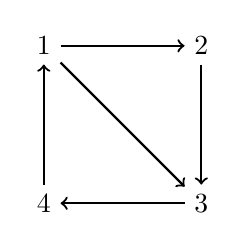
\begin{tikzpicture}
\node (atom1) at (0,2) {1};
\node (atom2) at (2,2) {2};
\node (atom3) at (2,0) {3};
\node (atom4) at (0,0) {4};
\draw[->, thick] (atom1)--(atom2);
\draw[->, thick] (atom2)--(atom3);
\draw[->, thick] (atom3)--(atom4);
\draw[->, thick] (atom4)--(atom1);
\draw[->, thick] (atom1) -- (atom3);
\end{tikzpicture}
\end{center}
Eftirfarandi mynd gæti lýst túlkun þar sem yfirgripið eru fyrstu fjórar heiltölurnar og \emph{R} er satt um (og aðeins satt um) eftirfarandi:
	\begin{center}
		\ntuple{1, 2}, 
		\ntuple{2, 3}, 
		\ntuple{3, 4}, 
		\ntuple{4, 1}, 
		\ntuple{1, 3}
	\end{center}
Við gætum líka tekið eftirfarandi mynd:

\begin{center}
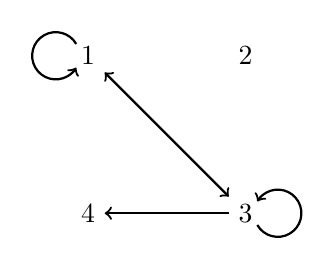
\begin{tikzpicture}
\node (atom1) at (0,2) {1};
\node (atom2) at (2,2) {2};
\node (atom3) at (2,0) {3};
\node (atom4) at (0,0) {4};
\draw[->, thick] (atom3)--(atom4);
\draw[->, thick] (atom1)+(-0.15,0.15) arc (-330:-30:.3); 
\draw[->, thick] (atom3)+(0.15,-0.15) arc (-150:150:.3); 
\draw[<->, thick] (atom1) -- (atom3);
\end{tikzpicture}
\end{center}
sem dæmi um túlkun með sama yfirgrip, þar sem umtak $R$ er:
	\begin{center}
		\ntuple{1, 3}, 
		\ntuple{3, 1}, 
		\ntuple{3, 4}, 
		\ntuple{1, 1},
		\ntuple{3, 3}
	\end{center}
Ef við viljum, þá getum við líka teiknað flóknari myndir. Við gætum til að mynda bætt nöfnum inn sem merkimiða á tiltekna hluti. Við gætum líka táknað umtak einsæta umsagnar með því að draga hring utan um þá hluti sem hún á að vera sönn um (og aðeins þá). Það sem mestu skiptir er að túlkunin tilgreini yfirgrip og umtak setninganna (og til hvaða hluta nöfnin eiga að vísa, ef við notum þau).

\chapter{Sannleikur í umsagnarökfræði}\label{s:TruthFOL}
Túlkanir segja okkur um hvaða hluti í yfirgripinu umsagnir eru sannar um og til hvaða hluta nöfnin sem við notum vísa. Þær segja okkur með öðrum orðum hvaða grunnsetningar eru sannar og hverjar ekki. Það sem okkur vantar þá er að geta sagt um \emph{allar} setningar í umsagnarökfræði hvort þær séu sannar eða ósannar---að einhverri túlkun gefinni.

Við lærðum í kafla \S\ref{s:FOLSentences} að það eru þrjár tegundir af setningum í umsagnarökfræði:
	\begin{ebullet}
		\item grunnsetningar
		\item setningar sem hafa setningatengi sem aðalvirkja
		\item setningar sem hafa magnara sem aðalvirkja
	\end{ebullet}
Við þurfum því að skilgreina hvað sannleikur í umsagnarökfræði er fyrir allar þessar þrjár gerðir setninga.	

Slík skilgreining verður, eðli málsins samkvæmt, að vera fullkomlega almenn. En í því skyni að gera umfjöllunina skýrari, þá mun ég á köflum notast við eftirfarandi túlkun:
	\begin{ekey}
		\item[\text{yfirgrip}] fólk fætt fyrir árið 2000\textsc{ce}
		\item[a] Aristóteles
		\item[d] Donald Trump
		\item[V] \gap{1} er vitur
		\item[R] \gap{1} fæddist á undan \gap{2}
	\end{ekey}
Þessi túlkun verður notuð sem dæmi þegar við á.	
\section{Grunnsetningar}
Sanngildi grunnsetninga er tiltölulega einfalt mál. Setningin \emph{Va} ætti að vera sönn ef og aðeins ef umsögnin \emph{V} er sönn um \emph{a}. Ef við miðum við þá túlkun sem gefin var hér að ofan, þá er þetta satt ef og aðeins ef Aristóteles er vitur. Aristóteles er vitur, svo setningin er sönn.\footnote{Það er að segja, ef við hunsum tíð sagnarinnar. Það eru til önnur rökfræðikerfi sem reyna að fanga tíðir sagna, en klassísk umsagnarökfræði er ekki ein af þeim.} Á sama hátt gætum við sýnt að setningin \emph{Vd} sé ósönn samkvæmt þessari túlkun.

Hvað með tvísæta umsagnirnar? \emph{Rad} er sönn ef og aðeins ef sá hlutur í yfirgripinu sem \emph{a} nefnir er fæddur á undan þeim hlut sem \emph{d} nefnir. Aristóteles fæddist vissulega á undan Donald Trump, svo \emph{Rad} er sönn. \emph{Raa} er ósönn, því Aristóteles fæddist ekki á undan Aristótelesi.

Það liggur því beint við að segja:
	\factoidbox{
		Ef \meta{R} er $n$-sæta umsögn og $\meta{a}_1, \meta{a}_{2}, \ldots, \meta{a}_{n}$ eru nöfn, þá er setningin $\meta{R}\meta{a}_{1}\meta{a}_{2}\ldots\meta{a}_{n}$ sönn samkvæmt tiltekinni túlkun, ef og aðeins ef R er sönn um þá hluti sem $\meta{a}_{1}, \meta{a}_{2}, \ldots, \meta{a}_{n}$ (í þessari röð) nefna samkvæmt þeirri sömu túlkun.
		}
Við megum þó ekki gleyma að það er til ein önnur gerð grunnsetninga, nefnilega setningar sem innihalda samsemdarmerkið. Um þær segjum við:
	\factoidbox{
		Ef $\meta{a}$ og $\meta{b}$ eru nöfn, þá er setningin $\meta{a} = \meta{b}$ sönn samkvæmt ákveðinni túlkun ef og aðeins ef
		 \meta{a} og \meta{b} nefna sama hlut samkvæmt þeirri sömu túlkun.
	}
Ef við skoðum aftur túlkunina sem gefin var hér að ofan, þá er setningin $a = d$ ósönn, þar eð \emph{a} nefnir Aristóteles en \emph{d} nefnir Donald Trump---og Aristóteles og Trump eru ekki sami hluturinn. Á hinn bóginn er $a = a$ sönn, þar sem Aristóteles er sami hluturinn og Aristóteles!

\section{Setningatengi}

Við lærðum í \S\ref{s:FOLSentences} að setningar í umsagnarökfræði eru smíðaðar úr einfaldari setningum með sömu setningatengjum og við kynntumst í setningarökfræðinni. Reglurnar sem ákvarða sannleika fyrir setningar í umsagnarökfræði sem hafa setningatengi sem aðalvirkja (en ekki magnara) eru því nákvæmlega þær sömu og fyrir setningar í setningarökfræði. Hér eru þær:
	\factoidbox{
		$\meta{A} \eand \meta{B}$ er sönn skv.\ tiltekinni túlkun \textbf{eff}\\ $\meta{A}$ og $\meta{B}$ eru báðar sannar skv.\ sömu túlkun \\ \\		
		$\meta{A} \eor \meta{B}$ er sönn skv.\ tiltekinni túlkun \textbf{eff}\\ annað hvort $\meta{A}$ er sönn eða $\meta{B}$ er sönn skv.\ sömu túlkun \\ \\
		$\enot \meta{A}$ er sönn skv.\ tiltekinni túlkun \textbf{eff}\\$\meta{A}$ er ósönn skv.\ sömu túlkun \\ \\
		$\meta{A} \eif \meta{B}$ er sönn skv.\ tiltekinni túlkun \textbf{eff}\\ annað hvort $\meta{A}$ er ósönn eða $\meta{B}$ er sönn skv.\ sömu túlkun \\ \\
		$\meta{A} \eiff \meta{B}$ er sönn skv.\ tiltekinni túlkun \textbf{eff}\\$\meta{A}$ hefur sama sanngildi og $\meta{B}$ skv.\ sömu túlkun
	}
En hvernig má vera að þetta séu sömu reglur? Skilgreindum við ekki sannleika í setningarökfræði með sanntöflum? Jú, en þrátt fyrir að vera á öðru formi, þá segja þessar reglur það sama. Við gætum meira að segja litið á þær sem \emph{lýsingu} á sanntöflunum okkar. Til dæmis, ef við myndum skoða sanntöfluna fyrir og-tengið, þá sæjum við að $\meta{A} \eand \meta{B}$ er bara sönn á þeirri línu þar sem \meta{A} er sönn og \meta{B} er sönn, en ósönn annars staðar---rétt eins og reglan fyrir og-tengið segir hér. Sama gildir um hinar reglurnar.

Hér eru nokkur dæmi um setningar til glöggvunar:
	
	\begin{earg}
		\item[\textbullet] $a = a \eand Va$ er sönn
		\item[\textbullet] $Rad \eand Vd$ er ósönn, því jafnvel þó $Rad$ sé sönn, þá er $Vd$ ósönn
		\item[\textbullet] $a = d \eor Va$ er sönn
		\item[\textbullet] $a \neq d$ er sönn
		\item[\textbullet] $Va \eand \enot( a= d \eand Rad)$ er sönn, því $Va$ er sönn og $a = d$ er ósönn
	\end{earg}

\section{Setningar með magnara sem aðalvirkja}\label{s:MainLogicalOperatorQuantifier}

Það sem greinir umsagnarökfræðina frá setningarökfræðinni eru þó auðvitað \emph{magnararnir} og það vill svo til að það er ekki alveg jafn auðvelt að skilgreina sannleika fyrir þá og maður myndi kannski halda. Hér er ein hugmynd: Við viljum segja að $\forall x Fx$ sé sönn eff $Fx$ er sönn um allt í yfirgripinu. Af hverju ekki bara að láta túlkunina sjá um þetta, enda segir hún til um það hvort $F$ sé satt um allt í yfirgripinu eða ekki?

En því miður er þessi lausn ekki nógu almenn. Munum að setningar í umsagnarökfræði eru byggðar upp í skrefum, úr öðrum setningum, og við viljum geta sagt um \emph{allar} setningar hvenær þær eru sannar og hvenær ekki. Hvað þá um $\forall x \exists y Lxy$ til að mynda? Þessi setning ætti að vera sönn ef og aðeins ef $\exists y Lxy$ er sönn um allt í yfirgripinu. En túlkunin getur ekki sagt okkur neitt um það. Við viljum því að það \emph{leiði af} túlkuninni og merkingu magnaranna að $\exists y Lxy$ sé sönn.

Hér er því önnur hugmynd. Við gætum reynt að segja að $\forall x \exists y Lxy$ sé sönn eff $\exists y L\meta{a}y$ er sönn fyrir \emph{öll} nöfn \meta{a} sem við höfum tiltekið. Á svipaðan hátt gætum við sagt að $\exists y L\meta{a}y$ sé sönn eff $L\meta{a}\meta{b}$ er sönn fyrir \emph{eitthvað} nafn \meta{b} í túlkuninni.xw

Þetta væri vissulega skref í rétta átt, en því miður dugir það ekki til. Til að sjá það, skoðum aftur túlkunina sem við tilgreindum í upphafi þessa kafla. Þar höfum við bara tvö nöfn, $a$ og $d$. En yfirgripið inniheldur allt fólk fætt fyrir árið 2000---sem eru að sjálfsögðu mun, mun fleiri! Við höfum hvorki vilja né getu til að nefna allt þetta fólk í yfirgripinu en viljum samt geta sagt eitthvað um það með mögnurum.

Hér er því þriðja hugmyndin: Það er vissulega rétt að við höfum ekki nefnt allt í yfirgripinu í túlkuninni, en \emph{fræðilega} séð væri það mögulegt. Það skiptir jú ekki máli hversu mörg nöfn við höfum í túlkuninni, við gætum alltaf bætt einu við í viðbót---víkkað túlkunina út. Skoðum þessa hugmynd aðeins betur áður en við gefum almenna skilgreiningu.

Í túlkuninni sem við höfum notað sem dæmi hingað til ætti setningin $\exists x Rdx$ að vera sönn. Það eru jú margir í yfirgripinu sem fæddust á eftir Donald Trump. Til dæmis Björk Guðmundsdóttir. Ef við myndum tímabundið víkka út túlkunina okkar og bæta nafninu $b$ sem vísaði til Bjarkar við túlkunina, þá myndi setningin $Rdb$ nú vera sönn (samkvæmt þessari nýju, útvíkkuðu túlkun). Það sýnir að $\exists x Rdx$ hlýtur að vera satt samkvæmt upprunalegu túlkuninni (munið: við bættum Björk ekki við yfirgripið, enda var hún þar þá þegar, heldur bættum við við \emph{nafni} sem vísaði til hennar).

Setningin $\exists x (Vx \eand Rxa)$ ætti líka að vera sönn. Sókrates var jú vitur og fæddist á undan Aristótelesi. Ef við bættum nýju nafni, $c$, við túlkunina og létum það vísa til Sókratesar, þá væri setningin $Vc \eand Rca$ greinilega sönn samkvæmt þessari útvíkkuðu túlkun. Rétt eins og áður, þá myndi það sýna að $\exists x (Vx \eand Rxa)$ hlýtur að vera sönn samkvæmt upprunalegu túlkuninni.

Skoðum eitt dæmi til viðbótar. Samkvæmt túlkuninni ætti $\forall x \exists y Rxy$ að vera ósönn setning. Hún segir að allir í yfirgripinu séu þannig að það sé einhver sem er fæddur á eftir þeim. Ef við prófuðum því að taka síðustu manneskjuna sem fæddist árið 1999 og úthluta henni nafni, segjum $l$, þá gætum við ekki fundið neinn annan, sem við getum til dæmis kallað $m$, í yfirgripinu sem er þannig að $Rlm$. Það skiptir engu máli hver í yfirgripinu fengi úthlutað nafninu $m$, þessi setning væri alltaf ósönn. Það sýnir að $\exists y Rly$ er ósönn samkvæmt upprunalegu túlkuninni.

Með þessi dæmi í huga, þá getum við loks gefið almenna skilgreiningu á sannleika fyrir setningar í umsagnarökfræði sem hafa magnara sem aðalvirkja. Þessi skilgreining er því miður ekki sérlega falleg og við þurfum að kynna til sögunnar nokkur ný hugtök áður en við byrjum. 

Segjum að \meta{A} sé formúla sem inniheldur að minnsta kosti eitt tilvik af breytunni \meta{x} og að \meta{x} sé óbundin í \meta{A}. Við skrifum þá:
$$\meta{A}(\ldots \meta{x} \ldots \meta{x} \ldots)$$
Segjum líka að \meta{c} sé nafn. Þá munum við skrifa:
$$\meta{A}(\ldots \meta{c} \ldots \meta{c} \ldots)$$
fyrir þá formúlu sem fæst með að skipta \meta{x} í \meta{A} út fyrir \meta{c} alls staðar þar sem \meta{x} kemur fyrir. Við köllum þessa formúlu \define{innsetningartilvik} af $\forall \meta{x}\meta{A}$ og $\exists\meta{x}\meta{A}$. Við köllum \meta{c} \define{innsetningarnafn}. Innsetningartilvik er með öðrum orðum sú formúla sem fæst með að taka magnara framan af annarri formúlu og skipta þeirri breytu sem magnarinn batt út fyrir eitthvað nafn. Formúlan
	$$\exists x (Rex \eiff Fx)$$
er því innsetningartilvik af formúlunni
	$$\forall y \exists x (Ryx \eiff Fx)$$
með innsetningarnafnið $e$.

Með þennan rithátt að vopni getum við loksins skilgreint sannleika fyrir setningar sem hafa magnara sem aðalvirkja. Við getum sagt að setningin $\forall \meta{x}\meta{A}(\ldots \meta{x} \ldots \meta{x} \ldots)$ sé sönn ef og aðeins ef $\meta{A}(\ldots \meta{c} \ldots \meta{c}\ldots)$ er sönn sama hvaða hlut í yfirgripinu nafnið $\meta{c}$ nefnir. Eins getum við sagt að setningin $\exists \meta{x}\meta{A}$ sé sönn ef og aðeins ef það er hægt að finna hlut í yfirgripinu og gefa honum nafnið \meta{c} þannig að setningin $\meta{A}(\ldots \meta{c} \ldots \meta{c} \ldots)$ sé sönn.

Með örlítið nákvæmari og formlegri hætti segjum við:
	\factoidbox{
		$\forall \meta{x}\meta{A}(\ldots \meta{x}\ldots\meta{x}\ldots)$ er sönn samkvæmt tiltekinni túlkun \textbf{eff}\\$\meta{A}(\ldots \meta{c} \ldots \meta{c}\ldots)$ er sönn fyrir \emph{hvaða} aðra túlkun sem útvíkkar upprunalegu túlkunina þannig að einhverjum hlut í yfirgripinu er gefið nafnið \meta{c} (án þess þó að breyta upprunalegu túlkuninni á nokkurn hátt annan)\\ \\
		$\exists \meta{x}\meta{A}(\ldots \meta{x}\ldots\meta{x}\ldots)$ er sönn samkvæmt tiltekinni túlkun \textbf{iff}\\ 
		$\meta{A}(\ldots \meta{c}\ldots\meta{c}\ldots)$ fyrir \emph{einhverja} aðra túlkun sem útvíkkar upprunalegu túlkunina þannig að einhverjum hlut í yfirgripinu er gefið nafnið \meta{c} (án þess þó að breyta upprunalegu túlkuninni á nokkurn hátt annan)
	}
Það eina sem skilgreiningin í kassanum hér að ofan gerir er að skilgreina---kannski of---nákvæmlega þessa óformlegu hugmynd um útvíkkun sem kynnt var hér að ofan. Hún kann kannski að virðast helstu óskýr og tyrfin, en vonandi er hugmyndin þar að baki það ekki.

\practiceproblems
\problempart
\label{pr.TorF1}
Skoðið eftirfarandi túlkun (og hafið í huga að það er engin skylda að hafa nöfn yfir allt í yfirgripinu):
	\begin{ebullet}
		\item yfirgripið samanstendur af Önnu og Jóni
		\item `$A$' er einsæta umsögn og sönn um Jón og Önnu
		\item `$B$' er einsæta umsögn og bara sönn um Önnu
		\item `$N$' er einsæta umsögn og ekki sönn um neitt
		\item `$j$' vísar til Jóns
	\end{ebullet}
Segið til um hvort eftirfarandi setningar séu sannar eða ósannar samkvæmt þessari túlkun:
\begin{earg}
\item $Bj$
\item $Aj \eiff \enot Nj$
\item $Nj \eif (Aj \eor Bj)$
\item $\forall x Ax$
\item $\forall x \enot Bx$
\item $\exists x(Ax \eand Bx)$
\item $\exists x(Ax \eif Nx)$
\item $\forall x(Nx \eor \enot Nx)$
\item $\exists x Bx \eif \forall x Ax$
\end{earg}

\problempart
Skoðið eftirfarandi túlkun:	
	\begin{ebullet}
		\item Yfirgripið samanstendur af Kasper, Jesper og Jónatan
		\item `$G$' er einsæta umsögn og sönn um Kasper, Jesper og Jónatan
		\item `$H$' er einsæta umsögn og bara sönn um Kasper
		\item `$M$' er einsæta umsögn og bara sönn um Jesper og Jónatan
		\item `$k$' vísar til Kaspers
		\item `$j$' vísar Jespers
	\end{ebullet}
Segið til um hvort eftirfarandi setningar séu sannar eða ósannar samkvæmt þessari túlkun:
\begin{earg}
\item $Hk$
\item $Hj$
\item $Mk \eor Mj$
\item $Gk \eor \enot Gk$
\item $Mk \eif Gk$
\item $\exists x Hx$
\item $\forall x Hx$
\item $\exists x \enot Mx$
\item $\exists x(Hx \eand Gx)$
\item $\exists x(Mx \eand Gx)$
\item $\forall x(Hx \eor Mx)$
\item $\exists x Hx \eand \exists x Mx$
\item $\forall x(Hx \eiff \enot Mx)$
\item $\exists x Gx \eand \exists x \enot Gx$
\item $\forall x\exists y(Gx \eand Hy)$
\end{earg}

\problempart
\label{pr.TorF3}
Skoðið umfjöllunina um myndræna framsetningu á túlkunum hér að ofan í \S\ref{s:Interpretations} og skoðið eftirfarandi túlkun:	
\begin{center}
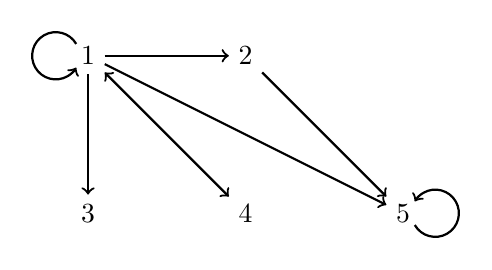
\begin{tikzpicture}
\node (atom1) at (0,2) {1};
\node (atom2) at (2,2) {2};
\node (atom4) at (0,0) {3};
\node (atom5) at (2,0) {4};
\node (atom6) at (4,0) {5};
\draw[->, thick] (atom1)+(-0.15,0.15) arc (-330:-30:.3); 
\draw[->, thick] (atom6)+(0.15,-0.15) arc (-150:150:.3); 
\draw[->, thick] (atom1) -- (atom2);
\draw[->, thick] (atom1) -- (atom4);
\draw[<->, thick] (atom1) -- (atom5);
\draw[->, thick] (atom1) -- (atom6);
\draw[->, thick] (atom2) -- (atom6);
\end{tikzpicture}
\end{center}
Segið til um hvort eftirfarandi setningar séu sannar eða ósannar samkvæmt þessari túlkun:
\begin{earg}
\item $\exists x Rxx$
\item $\forall x Rxx$
\item $\exists x \forall y Rxy$
\item $\exists x \forall y Ryx$
\item $\forall x \forall y \forall z ((Rxy \eand Ryz) \eif Rxz)$
\item $\forall x \forall y \forall z ((Rxy \eand Rxz) \eif Ryz)$
\item $\exists x \forall y \enot Rxy$
\item $\forall x(\exists y Rxy \eif \exists y Ryx)$
\item $\exists x \exists y (\enot x = y \eand Rxy \eand Ryx)$
\item $\exists x \forall y(Rxy \eiff x = y)$
\item $\exists x \forall y(Ryx \eiff x = y)$
\item $\exists x \exists y(\enot x = y \eand Rxy \eand \forall z(Rzx \eiff y = z))$
\end{earg}


\chapter{Merkingarfræðileg hugtök}
Að skilgreina sannleika í umsagnarökfræði var ansi snúið. En nú þegar við erum komin með skilgreininguna í hús getum við notað hana til að skilgreina önnur mikilvæg hugtök. Við höfum áður skilgreint sambærileg hugtök fyrir setningarökfræði í kafla \S\ref{s:semanticconcepts} en þau byggðu að sjálfsögðu á skilgreiningunni á sannleika fyrir setningarökfræði, sem byggðist á sanngildadreifingum, en ekki túlkunum. Þær eru í forgrunni hér. Að öðru leyti er ekkert nýtt á ferðinni.

\
\\Við notum táknið $\entails$ rétt eins og áður:
	$$\meta{A}_1, \meta{A}_2, \ldots, \meta{A}_n \entails\meta{C}$$
þýðir að það er ekki til nein túlkun sem gerir $\meta{A}_1, \meta{A}_2, \ldots, \meta{A}_n$  sanna og \meta{C} ósanna og við segjum að \meta{C} leiði rökfræðilega af $\meta{A}_1, \meta{A}_2, \ldots, \meta{A}_n$.

\
\\Ef $\meta{C}$ er sönn fyrir hvaða túlkun sem er, þá ritum við:
	$$\phantom{\meta{A}} \entails\meta{C}$$
Þá segjum við að $\meta{C}$ séu \define{röksannindi}. Röksannindi samsvarar klifun í setningarökfræði.

\
\\En á hinn bóginn, ef $\meta{A}$ er ósönn fyrir hvaða túlkun sem er, þá skrifum við:
$$\meta{A} \entails \phantom{\meta{C}}$$
Við köllum $\meta{A}$ þá \define{mótsögn}.

\
\\
Ef við viljum segja að það sé \emph{ekki} satt að $\meta{A}_1, \ldots, \meta{A}_n \entails \meta{C}$, þá strikum við yfir táknið fyrir rökfræðilega afleiðingu og segjum: 
$$\meta{A}_1, \meta{A}_2, \ldots, \meta{A}_n \nentails\meta{C}$$
Þetta þýðir að er til túlkun sem er þannig að setningarnar $\meta{A}_1,\ldots, \meta{A}_n$ eru allar sannar, en $\meta{C}$ er ósönn.
\
\\Tvær setningar í umsagnarökfræði \meta{A} og \meta{B} er \define{rökfræðilega jafngildar} eff þær eru sannar í nákvæmlega sömu túlkunum. Það er að segja, ef $\meta{A}\entails\meta{B}$ og $\meta{B}\entails\meta{A}$.

\
\\Eitthvert safn af setningum í umsagnarökfræði eru \define{rökfræðilega samkvæmar} ef og aðeins ef til er einhver túlkun þar sem þær eru allar sannar. Þær eru svo loks \define{rökfræðilega ósamkvæmar} eff engin slík túlkun er til.

\chapter{Að vinna með túlkanir}
\label{sec.UsingModels}

\section{Röksannindi og mótsagnir}
Gerum ráð fyrir að við viljum sýna að $\exists xAxx \eif Bd$ séu \emph{ekki} röksannindi. Í samræmi við skilgreininguna þurfum við þá að sýna að setningin sé ekki sönn fyrir allar túlkanir; það er að segja, að hún sé ósönn fyrir einhverja túlkun. Ef við getum því fundið eina einustu túlkun þar sem setningin er ósönn, þá höfum við sýnt að setningin sé ekki röksannindi.

Hvernig ættum við þá að bera okkur að? Við vitum að $\exists xAxx \eif Bd$ er ósönn, ef forliðurinn ($\exists x Axx$) er sannur og bakliðurinn ($Bd$) er ósannur. Við þurfum því að \emph{búa til} túlkun sem er þannig að þessi skilyrði eru uppfyllt. Við byrjum á því að tilgreina yfirgrip. Það er auðveldast að reyna að halda yfirgripinu eins litlu og mögulegt er, svo við bætum bara einum hlut við það. Segjum bara Dalvík.
	\begin{ekey}
		\item[\text{yfirgrip}] Dalvík
	\end{ekey}
Munum: Við erum að reyna að gera setninguna $Bd$ ósanna og við höfum bara einn hlut í yfirgripinu. Við erum því nauðbeygð til að láta nafnið $d$ vísa til Dalvíkur. 
	\begin{ekey}
		\item[d] Dalvík
	\end{ekey}
Munum líka að við viljum gera $\exists x Axx$ sanna. Við gætum tilgreint umtak þessarar umsagnar beint og sagt að hún eigi að innhalda parið $\ntuple{Dalvík, Dalvík}$. En við getum líka gert það óbeint með að tiltaka einhverja umsögn í mæltu máli sem er þannig að Dalvík stendur í þeim venslum við Dalvík. Til dæmis: 
	\begin{ekey}
		\item[A] \gap{1} er jafn stór og \gap{2}
	\end{ekey}
$Add$ er sönn samkvæmt þessari túlkun, enda er Dalvík jafn stór og Dalvík og því er $\exists x Axx$ líka sönn. En hvernig gerum við $Bd$ ósanna? Ein leið væri að tiltaka beint að Dalvík sé ekki í umtaki $B$, til dæmis með að láta B vera tóma umsögn (það er að segja, ekki sanna um neitt). En við gætum líka tiltekið þetta óbeint, til dæmis svona:
	\begin{ekey}
		\item[B] \gap{1} er í Færeyjum
	\end{ekey}
Hér höfum við þá túlkun þar sem $\exists x Axx$ er sönn en $Bd$ er ósönn. Það er því til túlkun þar sem $\exists x Axx \eif Bd$ er ósönn. Setningin er því ekki röksannindi.

Við getum líka auðveldlega sýnt að $\exists xAxx \eif Bd$ er ekki mótsögn. Við þurfum bara að tilgreina túlkun þar sem $\exists xAxx \eif Bd$ er sönn. Til þess þurfum við að finna túlkun þar sem annað hvort $\exists x Axx$ er ósönn eða $Bd$ er sönn. Hér er túlkun þar sem hið seinna gildir:
	\begin{ekey}
		\item[\text{yfirgrip}] Dalvík
		\item[d] Dalvík
		\item[A] \gap{1} er jafn stór og \gap{2}
		\item[B] \gap{1} er á Íslandi
	\end{ekey}
Þetta sýnir að það er til túlkun þar sem $\exists xAxx \eif Bd$ er sönn. $\exists xAxx \eif Bd$ er því ekki mótsögn.

\section{Rökfræðilegt jafngildi}

Segjum nú að við viljum sýna að $\forall x Sx$' og `$\exists x Sx$ séu ekki rökfræðilega jafngildar setningar. Í því skyni þurfum við að smíða túlkun þar sem setningarnar hafa ólík sanngildi; þar sem ein er sönn og hin er ósönn. Við viljum halda yfirgripinu litlu, en við getum ekki haft bara einn hlut í því (ef yfirgripið inniheldur bara einn hlut, þá hljóta þessar setningar báðar að vera sannar. Hugsið um af hverju!) Við þurfum því að minnsta kosti tvo hluti í yfirgripinu. Tökum sem dæmi:
	\begin{ekey}
		\item[\text{yfirgrip}] John Coltrane, Miles Davis
	\end{ekey}
Við getum gert $\exists x Sx$ sanna með því að gæta þess að eitthvað sé í umtaki $S$ og $\forall x Sx$ ósanna með því að hafa eitthvað í yfirgripinu sem er ekki í umtaki $S$. Til dæmis:
	\begin{ekey}
		\item[S] \gap{1} spilar á saxófón
	\end{ekey}
$\exists x Sx$ er sönn, því John Coltrane er saxófónleikari og því í umtaki $S$. Takið þó eftir því að við höfum ekki kynnt nein nöfn til sögunnar. Setningin er sönn af því að við getum víkkað út túlkunina okkar með nýju nafni sem vísar til Johns Coltrane, $c$, og þá segir skilgreiningin okkar á sannleika í umsagnarökfæðpi að af því að $Sc$ sé sönn í þessari nýju útvíkkuðu túlkun, þá sé $\exists x Sx$ sönn í upprunalegu túlkuninni.

Svipað má segja um $\forall x Sx$. Hún er ósönn, því við getum víkkað út túlkunina þannig að nýtt nafn, $c$, vísar til Miles Davis. $Sc$ er ósönn í þessari túlkun og því er $\forall x Sx$ ósönn í upprunalegu túlkuninni. Það sem við höfum gert er að finna túlkun sem er \emph{mótdæmi} við þá fullyrðingu að $\forall x Sx$ og $\exists x Sx$ séu rökfræðilega jafngildar setningar.
	
	\factoidbox{
		Til að sýna að $\meta{A}$ séu ekki röksannindi er nóg að finna túlkun þar sem $\meta{A}$ er ósönn.
		
		Til að sýna að $\meta{A}$ sé ekki mótsögn er nóg að finna túlkun þar sem $\meta{A}$ er sönn.
		
		Til að sýna að $\meta{A}$ og $\meta{B}$ séu ekki rökfræðilega jafngild, er nóg að finna túlkun þar sem setningarnar hafa ólík sanngildi.
	}

\section{Gildi, rökfræðileg afleiðing og samkvæmni}
Til að meta gildi, rökfræðilega afleiðingu eða samkvæmni setninga þurfum við oftast að finna túlkun sem ákvarðar sanngildi fleiri en einnar setningar í einu. 

Skoðum til dæmis eftirfarandi rökfærslu á máli umsagnarökfræði:
	$$\exists x(Mx \eif Ml) \therefore \exists x Mx \eif Ml$$
Ef við viljum sýna að þessi rökfærsla sé ógild, þá þurfum við að finna túlkun þar sem forsendan er sönn en niðurstaðan ósönn. Niðurstaðan er skilyrðissetning, svo ef hún er ósönn, þá hlýtur forliðurinn að vera sannur og bakliðurinn ósannur. Það getur bara verið ef yfirgripið inniheldur að minnsta kosti tvo hluti (af hverju?). Hér er tillaga:
	
\begin{ekey}
	\item[\text{yfirgrip}] Svarthöfði, Logi Geimgengill
	\item[M] \gap{1} lét freistast af myrku hlið Máttarins
	\item[l] Logi Geimgengill
\end{ekey}
Þar sem Logi lét aldrei freistast af myrku hlið Máttarins er $Ml$ ósönn, samkvæmt þessari túlkun. En það gerði Svarthöfði vissulega. Svo $\exists x Mx$ er sönn. Þar af leiðandi er $\exists x Mx \eif Ml$ ósönn.

En er forsendan sönn samkvæmt þessari túlkun? Já, tökum fyrst eftir því að $Ml \eif Ml$ er sönn (og raunar röksannindi!). En þá hlýtur $\exists x (Mx \eif Ml)$ að vera sönn. Svo það er til túlkun þar sem forsendan er sönn, en niðurstaðan ósönn, og því er þessi rökfærsla ógild.

Tökum líka eftir því að við höfum í leiðinni sýnt að $\exists x Mx \eif Ml$ leiðir \emph{ekki} rökfræðilega af $\exists x(Mx \eif Ml)$, það er að segja, að $\exists x(Mx \eif Ml) \nentails \exists x Mx \eif Ml$. Við höfum líka sýnt að setningarnar $\exists x(Mx \eif Ml)$ og $\enot(\exists x Mx \eif Ml)$ eru rökfræðilega samkvæmar.

Skoðum annað dæmi:
$$\forall x \exists y Fxy \therefore \exists y \forall x Fxy$$
Ef við viljum sýna að þessi rökfærsla sé ógild, þá þurfum við að sýna að til sé túlkun þar sem forsendan er sönn en niðurstaðan ósönn. Hér er ein slík túlkun:
\begin{ekey}
	\item[\text{yfirgrip}] Öll systkini
	\item[F] \gap{1} er systkini \gap{2}
\end{ekey}
Forsendan er greinilega sönn samkvæmt þessari túlkun. Yfirgripið inniheldur öll systkini. Það skiptir því ekki máli hvaða systkini við veljum, að minnsta kosti eitt af systkinum þeirra er líka í yfirgripinu (því það er jú ekki hægt að vera systkini án þess að eiga systkini!). $\forall x \exists y Fxy$ er því sönn. En niðurstaðan er greinilega ósönn, því hún væri bara sönn ef það væri eitthvað systkini í yfirgripinu sem er þannig að það er systkini allra annarra. Það er ekkert slíkt „ofursystkini“. Rökfærslan er því ógild. Við sjáum líka strax að $\forall x \exists y Fxy$ og $\enot\exists y \forall x Fxy$ eru samkvæmar og að $\forall x \exists y Fxy \nentails \exists y \forall x Fxy$

Síðasta dæmið er dálítið öðruvísi. Munum að í \S\ref{s:Interpretations} sáum við að hægt er að tiltaka túlkanir myndrænt. Hér er ein slík túlkun:
\begin{center}
	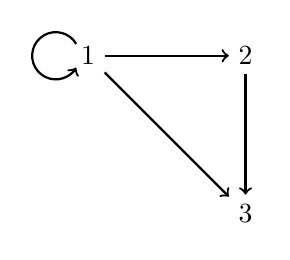
\begin{tikzpicture}
	\node (atom1) at (0,2) {1};
	\node (atom2) at (2,2) {2};
	\node (atom3) at (2,0) {3};
	\draw[->, thick] (atom1)--(atom2);
	\draw[->, thick] (atom1)--(atom3);
	\draw[->, thick] (atom1)+(-0.15,0.15) arc (-330:-30:.3); 
	\draw[->, thick] (atom2) -- (atom3);
	\end{tikzpicture}
\end{center}
Yfirgrip þessarar túlkunar eru fyrstu þrjár heiltölurnar og $Rxy$ er sönn um \emph{x} og \emph{y} ef og aðeins ef það er ör frá \emph{x} til \emph{y} á myndinni. Hér eru nokkrar setningar sem eru sannar samkvæmt þessari túlkun:
\begin{ebullet}
	\item $\forall x \exists y Ryx$ 
	\item $\exists x \forall y Rxy$ \hfill vitni 1
	\item $\exists x \forall y (Ryx \eiff x = y)$ \hfill vitni 1
	\item $\exists x \exists y \exists z (\enot y = z \eand Rxy \eand Rzx)$ \hfill vitni 2
	\item $\exists x \forall y \enot Rxy$ \hfill vitni 3
	\item $\exists x (\exists y Ryx \eand \enot \exists y Rxy)$ \hfill vitni 3
\end{ebullet}
Þetta sýnir að allar þessar setningar eru rökfræðilega samkvæmar. Við getum notfært okkur það til að búa til fleiri og fleiri \emph{ógildar} rökfærslur. Til dæmis:
\begin{align*}
\forall x \exists y Ryx, \exists x \forall y Rxy  &\therefore  \forall x \exists y Rxy\\
\exists x \forall y Rxy, \exists x \forall y \enot Rxy & \therefore \enot \exists x \exists y \exists z (\enot y = z \eand Rxy \eand Rzx)
\end{align*}
og margar fleiri.
\factoidbox{
	Ef til er túlkun þar sem $\meta{A}_1, \meta{A}_2, \ldots, \meta{A}_n$  eru allar sannar og $\meta{C}$ ósönn, þá er:
	\begin{ebullet}
		\item$\meta{A}_1, \meta{A}_2, \ldots, \meta{A}_n \therefore \meta{C}$ \emph{ógild}; og
	\item $\meta{A}_1, \meta{A}_2, \ldots, \meta{A}_n \nentails \meta{C}$; og
	\item 
	 $\meta{A}_1, \meta{A}_2, \ldots, \meta{A}_n, \enot \meta{C}$ eru rökfræðilega samkvæmar.
\end{ebullet}}
Túlkun sem sýnir að tiltekin setning sé \emph{ekki} röksannindi eða að einhverja setningu leiði ekki af annarri er kölluð \emph{gagntúlkun} eða \emph{gagnlíkan}.

Ég vil að lokum minna á sambandið milli gildis og rökfræðilegrar afleiðingar. Umsagnarökfræðin er umtaksmál og hunsar því alls konar blæbrigði mannlegs máls. Það geta því verið aðrar ástæður fyrir því að rökfærsla er gild en umsagnarökfræðin getur fangað. Hér er dæmi:
\begin{earg}
	\item[] Allir kettir eru dauðlegir
	\item[Þar af leiðir:] Allar læður eru dauðlegar
\end{earg}
Þetta er gild rökfærsla. Allar læður eru kettir, svo það er ómögulegt fyrir forsenduna að vera sanna og niðurstöðuna ósanna. Við gætum reynt að þýða þessa rökfærslu yfir á táknmál umsagnarökfræði svona:
$$\forall x(Kx \eif Dx) \therefore \forall x(Lx \eif  Dx)$$
Það er hins vegar lítið mál að finna gagntúlkun sem sýnir að $\forall x (Kx \eif Dx) \nentails \forall x (Lx \eif Dx)$. (Finnið slíka túlkun.) Það væri því rangt að draga þá ályktun að þessi rökfærsla sé ógild, bara af því að til er gagntúlkun fyrir samsvarandi rökfærslu á máli setningarökfræði. Slík þýðing gengur bara ef ekkert mikilvægt tapast í þýðingunni.

\practiceproblems

\problempart
\label{pr.Contingent}
Sýnið að eftirfarandi setningar séu hvorki röksannindi né mótsagnir:
\begin{earg}
\item  $Da \eand Db$
\item  $\exists x Txh$
\item  $Pm \eand \enot\forall x Px$
\item $\forall z Jz \eiff \exists y Jy$
\item $\forall x (Wxmn \eor \exists yLxy)$
\item $\exists x (Gx \eif \forall y My)$
\item $\exists x (x = h \eand x = i)$
\end{earg}

\problempart
\label{pr.NotEquiv}
Sýnið að eftirfarandi setningapör séu ekki rökfræðilega jafngild.
\begin{earg}
\item $Ja$, $Ka$
\item $\exists x Jx$, $Jm$
\item $\forall x Rxx$, $\exists x Rxx$
\item $\exists x Px \eif Qc$, $\exists x (Px \eif Qc)$
\item $\forall x(Px \eif \enot Qx)$, $\exists x(Px \eand \enot Qx)$
\item $\exists x(Px \eand Qx)$, $\exists x(Px \eif Qx)$
\item $\forall x(Px\eif Qx)$, $\forall x(Px \eand Qx)$
\item $\forall x\exists y Rxy$, $\exists x\forall y Rxy$
\item $\forall x\exists y Rxy$, $\forall x\exists y Ryx$
\end{earg}



\problempart
Sýnið að eftirfarandi setningar séu samkvæmar:
\begin{earg}
\item $Ma, \enot Na, Pa, \enot Qa$
\item $Lee, Leg, \enot Lge, \enot Lgg$
\item $\enot (Ma \eand \exists x Ax), Ma \eor Fa, \forall x(Fx \eif Ax)$
\item $Ma \eor Mb, Ma \eif \forall x \enot Mx$
\item $\forall y Gy, \forall x (Gx \eif Hx), \exists y \enot Iy$
\item $\exists x(Bx \eor Ax), \forall x \enot Cx, \forall x\bigl[(Ax \eand Bx) \eif Cx\bigr]$
\item $\exists x Xx, \exists x Yx, \forall x(Xx \eiff \enot Yx)$
\item $\forall x(Px \eor Qx), \exists x\enot(Qx \eand Px)$
\item $\exists z(Nz \eand Ozz), \forall x\forall y(Oxy \eif Oyx)$
\item $\enot \exists x \forall y Rxy, \forall x \exists y Rxy$
\item $\enot Raa$, $\forall x (x=a \eor Rxa)$
\item $\forall x\forall y\forall z(x=y \eor y=z \eor x=z)$, $\exists x\exists y\ \enot x= y$
\item $\exists x\exists y(Zx \eand Zy \eand x=y)$, $\enot Zd$, $d=e$
\end{earg}

\problempart
Sýnið að eftirfarandi rökfærslur séu ógildar:
\begin{earg}
\item $\forall x(Ax \eif Bx) \therefore \exists x Bx$
\item $\forall x(Rx \eif Dx), \forall x(Rx \eif Fx) \therefore \exists x(Dx \eand Fx)$
\item $\exists x(Px\eif Qx) \therefore \exists x Px$
\item $Na \eand Nb \eand Nc \therefore \forall x Nx$
\item $Rde, \exists x Rxd \therefore Red$
\item $\exists x(Ex \eand Fx), \exists x Fx \eif \exists x Gx \therefore \exists x(Ex \eand Gx)$
\item $\forall x Oxc, \forall x Ocx \therefore \forall x Oxx$
\item $\exists x(Jx \eand Kx), \exists x \enot Kx, \exists x \enot Jx \therefore \exists x(\enot Jx \eand \enot Kx)$
\item $Lab \eif \forall x Lxb, \exists x Lxb \therefore Lbb$
\item $\forall x(Dx \eif \exists y Tyx) \therefore \exists y \exists z\ \enot y= z$
\end{earg}

\chapter{Takmarkanir túlkana og umsagnarökfræðinnar}

\section{Röksannindi og mótsagnir}
Við getum sýnt að setning sé \emph{ekki} röksannindi með því að finna bara eina einustu túlkun sem sýnir að setningin sé ósönn. En ef við viljum á hinn bóginn sýna að setning \emph{sé} röksannindi þá skiptir ekki máli hversu margar túlkanir við finnum þar sem hún er sönn, það er alltaf möguleiki að til sé einhver önnur túlkun þar sem hún er ósönn. Við þyrftum því að geta hugsað upp óendanlega margar túlkanir!

Stundum getum við þó neglt niður tiltölulega auðveldlega hvernig allar túlkanir fyrir tilteknar setningar hljóta að vera. Til dæmis, þá er tiltölulega auðvelt að sýna að $Raa\eiff Raa$ séu röksannindi: 
	\begin{quote}
		\label{allmodels1}
		Túlkun fyrir tiltekna setningu verður að tiltaka merkinga allra nafna sem kemur fyrir í henni. Ef $Raa$ er sönn í tiltekinni túlkun, þá er $Raa \eiff Raa$ sönn í þeirri túlkun. En ef $Raa$ er ósönn í einhverri túlkun, þá er $Raa \eiff Raa$ sönn í þeirri túlkun. Þetta eru einu möguleikarnir. $Raa \eiff Raa$ er því sönn fyrir allar túlkanir. Setningin er því röksannindi.
	\end{quote}
Þetta er gild rökfærsla og niðurstaða hennar er sönn. En þetta er auðvitað ekki rökfærsla \emph{á máli umsagnarökfræði}, heldur á mæltu máli \emph{um} umsagnarökfræði---þetta er rökfærsla á framsetningarmálinu.

Takið líka eftir því að setningin inniheldur enga magnara og við þurfum því ekki að spá neitt sérstaklega í því hvernig túlka beri $a$ eða $R$. Það eina sem skipti máli var að \emph{sama hvernig við túlkum þessi tákn, þá hefði $Raa$ eitthvað sanngildi}. Þessi rökfærsla hefði allt eins getað verið um setningar í setningarökfræði.	

Skoðum annað dæmi. Setningin $\forall x(Rxx\eiff Rxx)$ ætti að sjálfsögðu að vera röksannindi, rétt eins og fyrra dæmi. En það er ekki jafn auðvelt að sýna af hverju. Við getum ekki sagt að $Rxx \eiff Rxx$ sé satt fyrir allar túlkanir, því $Rxx \eiff Rxx$ er ekki einu sinni setning í umsagnarökfræði (\emph{x} er breyta, ekki nafn.) Við verðum því að reyna rökfærslu á borð við þessa:
	\begin{quote}
		Veljum einhverja túlkun af handahófi. Veljum svo eitthvað stak úr yfirgripinu---köllum það bara „S“. Víkkum svo út túlkunina sem við völdum þannig að nafnið $c$ vísi til S. Þá er $Rcc$ annað hvort sönn eða ósönn. Ef $Rcc$ er sönn, þá er $Rcc \eiff Rcc$ sönn. En ef $Rcc$ er ósönn, þá er $Rcc \eiff Rcc$ líka sönn. Svo hvort heldur sem er, þá er $Rcc$ sönn. En þar sem við völdum túlkun og S af handahófi, þá skiptir það engu máli hvernig við víkkum túlkunina sem við völdum út, $Rcc \eiff Rcc$ verður sönn. En þá er $\forall x (Rxx \eiff Rxx)$ sönn samkvæmt túlkuninni sem við völdum og af því að við völdum hana af handahófi, þá er $\forall x (Rxx \eiff Rxx)$ sönn fyrir allar túlkanir og er því röksannindi.
	\end{quote}
Þetta er ansi langdregið. En því miður er ekkert annað sem við getum gert. Ef við viljum sýna að setning séu röksannindi, þá eigum við engra annarra kosta völ en að sýna eitthvað um allar túlkanir og það er enginn hægðarleikur. Þetta gildir að sjálfsögðu líka um ýmis önnur tilfelli. Til dæmis ef við viljum sýna að:
	\begin{ebullet}
		\item setning sé mótsögn; hér þarf að sýna að hún sé ósönn í öllum túlkunum. 
		\item að tvær setningar séu rökfræðilega jafngildar; hér þurfum við að sýna að þær hafi sama sanngildi í öllum túlkunum.
		\item að eitthvað safn setninga sé ósamkvæmt; hér þurfum við að sýna að ekki sé til túlkun þar sem setningarnar eru allar sannar, það er, að sýna að í hverri einustu túlkun sé að minnsta kosti einn setninganna ósönn.
		\item að rökfærsla sé gild; hér þarf að sýna að niðurstaðan sé sönn í öllum túlkunum þar sem forsendurnar eru sannar.
		\item að einhverja setningu leiði af öðrum setningum.
	\end{ebullet}
Það er mikill munur á þessu og því sem við höfum áður kynnst. Sannleikur setninga í setningafræði er skilgreindur með sanngildadreifingum og hver setning hefur einungis endanlegan fjölda af mögulegum sanngildadreifingum. Við getum notað sanntöflur til að fá yfirsýn yfir allar þessar dreifingar og eru þær í raun aðferð til að meta sanngildi allra setninga í setningarökfræði á vélrænan hátt og óbrigðulan hátt. Við getum með öðrum orðum reiknað út sanngildi allra setninga í setningarökfræði. \emph{En það er ekki til nein slík aðferð í tilfelli umsagnarökfræði}.\footnote{Hér þurfum við samt að fara dálítið varlega. Það hefði vel verið mögulegt að slík almenn aðferð hefði verið til, þrátt fyrir að mögulegar túlkanir séu óendanlega margar. Það er ekki eina ástæðan fyrir þessum vanda. Hins vegar sönnuðu Alonso Church og Alan Turing um miðjan fjórða áratug síðustu aldar að slík aðferð er ekki til.} Umsagnarökfræði er, eins og sagt er, óúrskurðanleg (e.\ \emph{undecidable}). Þetta þýðir þó ekki að það séu til sannar setningar sem umsagnarökfræðin getur ekki sannað, bara að það er ekki til nein aðferð til að finna slíka sönnun. Við höfum þó ekki enn kynnt sannanir til sögunnar fyrir umsagnarrökfræðina, en það er efni næsta kafla.
%!TEX root = forallxcam.tex
\part{Náttúruleg afleiðsla fyrir umsagnarökfræði}
\label{ch.NDFOL}


\chapter{Grunnreglur náttúrulegrar afleiðslu fyrir umsagnarökfræði}\label{s:BasicFOL}

Táknmál umsagnarökfræði notar öll sömu setningatengin og setningarökfræðin. Sannanir í umsagnarökfræði munu því líka nota sömu reglur sannanir í setningarökfræði, bæði grunnreglurnar og afleiddar reglur (sjá \S\ref{ch.NDTFL}). Við munum líka nota sömu sönnunarfræðilegu hugtök og setningarökfræðin studdist við, og voru kynnt til sögunnar í þeim kafla, einkum og sér í lagi táknið „$\proves$“. Við þurfum hins vegar nýjar reglur fyrir magnarana og samsemdarmerkið.

Rétt eins og í tilfelli setningarökfræði, þá skilgreinum við innleiðingar- og eyðingarreglur fyrir hvert tákn. 

\section{Almagnaraeyðing}

Ef við vitum að allt sé $F$, þá getum við dregið þá ályktun að sérhver tiltekinn hlutur sé $F$---nefndu það, sá hlutur er $F$. Það er að segja ef allt er $F$, þá er $a$ líka $F$, og $b$, og $c\ldots$ Eftirfarandi ætti því að vera í lagi:

\begin{proof}
	\hypo{a}{\forall xRxxd}
	\have{c}{Raad} \Ae{a}
\end{proof}
Hér höfum við $\forall xRxxd$ sem forsendu, og fáum línu 2 með því að fjarlægja almagnarann og setja nafnið „$a$“ í stað breytunnar $x$, allstaðar þar sem hún kemur fyrir. Eftirfarandi ætti líka að vera í lagi:
\begin{proof}
	\hypo{a}{\forall xRxxd}
	\have{c}{Rddd} \Ae{a}
\end{proof}
Hér höfum við gert það sama, nema við höfum skipt út $x$ fyrir „$d$“ allstaðar þar sem $x$ kemur fyrir. Við hefðum getað gert slíkt hið sama fyrir hvaða nafn sem er annað, enda hlýtur það sem gildir um allt í yfirgripinu líka að gilda um allt sem við höfum nafn yfir, því það er jú hluti af yfirgripinu.

Almennt form almagnaraeyðingar ($\forall$E) er því þetta:

\factoidbox{
\begin{proof}
	\have[m]{a}{\forall \meta{x}\meta{A}(\ldots \meta{x} \ldots \meta{x}\ldots)}
	\have[\ ]{c}{\meta{A}(\ldots \meta{c} \ldots \meta{c}\ldots)} \Ae{a}
\end{proof}}Þessi ritháttur var kynntur til sögunnar í \S\ref{s:TruthFOL}. Í stuttu máli, þá merkir $\meta{A}(\ldots \meta{x} \ldots \meta{x}\ldots)$ formúlu þar sem breytan $\meta{x}$ kemur fyrir að minnsta kosti einu sinni fyrir í formúlunni $\meta{A}$ og $\meta{x}$ er óbundin, og $\meta{A}(\ldots \meta{c} \ldots \meta{c}\ldots)$ merkir formúlu þar sem öllu $\meta{x}$-unum í $\meta{A}(\ldots \meta{x} \ldots \meta{x}\ldots)$ hefur verið skipt út fyrir $\meta{c}$. Þetta þýðir sem sagt bara að þegar við beitum reglunni, þá tökum við almagnarann framan af, og skiptum út öllum breytunum sem hann bindur út fyrir eitthvað nafn. 

Við megum þó ekki gleyma að við getum \emph{bara} beitt þessari reglu, rétt eins og gildir um allar eyðingarreglur, þegar almagnarinn er aðalvirkinn í setningunni. Eftirfarandi er því \emph{ekki} leyfilegt: 

\begin{proof}
	\hypo{a}{\forall x Bx \eif Bt}
	\have{c}{Bj \eif Bt}\by{óleyfileg tilraun til að nota $\forall$E}{a}
\end{proof}
Hér er „$\forall x$“ ekki aðalvirkinn í línu 1, heldur „$\eif$“. Þessi rökfærsla er ógild (forsendan er nauðsynlega sönn, en niðurstaðan ekki. Það sýnir að eitthvað hefur farið úrskeiðis). Þetta eru mjög algeng mistök byrjenda, svo það er vel þess virði að taka vel eftir þessu.

\section{Innleiðing tilvistarmagnara}
Ef við vitum að einhver tiltekinn hlutur er \emph{F}, þá getum við dregið þá ályktun að eitthvað sé \emph{F}---nefnilega það sem við vissum að væri \emph{F}. Eftirfarandi ætti því að vera í lagi:
\begin{proof}
	\hypo{a}{Raad}
	\have{b}{\exists x Raax} \Ei{a}
\end{proof}
Hér höfum við skipt út nafninu „$d$“ fyrir breytuna „$x$“ og bundið hana svo við magnara. Við hefðum líka getað farið aðra leið:
\begin{proof}
	\hypo{a}{Raad}
	\have{c}{\exists x Rxxd} \Ei{a}
\end{proof}
Hér höfum við skipt út nafninu „$a$“ út á tveimur stöðum fyrir breytuna $x$ og bundið hana við magnara. Hér hefðum við ekki þurft að skipta út nafninu „$a$“ á báðum stöðum: Ef Ólafur elskar sjálfan sig, þá er jú einhver sem elskar Ólaf. Eftirfarandi er því líka leyfilegt: 

\begin{proof}
	\hypo{a}{Raad}
	\have{d}{\exists x Rxad} \Ei{a}
\end{proof}
Hér höfum við skipt út nafninu „$a$“ fyrir $„x“$ á öðrum af tveimur stöðum þar sem það kemur fyrir, og svo bundið hana með tilvistarmagnara. Þessi dæmi liggja að baki almennu formi reglunnar, en til að geta gefið slíkt form þurfum við fyrst að að kynna til sögunnar nýjan rithátt, líkan þeim sem við notuðum hér að ofan.

Hann er svona: Ef $\meta{A}$ er formúla þar sem nafnið $\meta{c}$ kemur fyrir, þá getum við skrifað $$\meta{A}(\ldots \meta{c} \ldots \meta{c}\ldots)$$ til að gefa það til kynna. Við getum svo skrifað $$\meta{A}(\ldots \meta{x} \ldots \meta{c}\ldots)$$ til að tákna formúlu þar sem sumum (og hugsanlega öllum) $\meta{c}$-unum í
$\meta{A}$ hefur verið skipt út fyrir breytuna $\meta{x}$.

Með þennan rithátt að vopni, þá getum við loks gefið almennt form reglunnar:
\factoidbox{
\begin{proof}
	\have[m]{a}{\meta{A}(\ldots \meta{c} \ldots \meta{c}\ldots)}
	\have[\ ]{c}{\exists \meta{x}\meta{A}(\ldots \meta{x} \ldots \meta{c}\ldots)} \Ei{a}
\end{proof}
þar sem \meta{x} má ekki koma fyrir í $\meta{A}$ (\ldots \meta{c} \ldots \meta{c}\ldots)}

Þessi síðasta klausa er til að tryggja að táknrunan sem verður til við skiptinguna sé setning í umsagnarökfræði. Eftirfarandi er því leyfilegt:
\begin{proof}
	\hypo{a}{Raad}
	\have{d}{\exists x Rxad} \Ei{a}
	\have{e}{\exists y \exists x Rxyd} \Ei{d}
\end{proof}
En svona er bannað:
\begin{proof}
	\hypo{a}{Raad}
	\have{d}{\exists x Rxad} \Ei{a}
	\have{e}{\exists x \exists x Rxxd}\by{óleyfileg tilraun til að nota $\exists$I}{d}
\end{proof}
Táknrunan á línu 3 inniheldur breytu sem er innan sviðs tveggja magnara sem báðir reyna að stjórna henni, og því er hún ekki setning á táknmáli umsagnarökfræði. Klausan sem við bættum við regluna kemur í veg fyrir að þetta geti gerst.

\section{Tóm yfirgrip}\label{tomtyfirgrip}
Eftirfarandi sönnun notar báðar reglurnar sem við höfum kynnst fram að þessu:
	\begin{proof}
		\hypo{a}{\forall x Fx}
		\have{in}{Fa}\Ae{a}
		\have{e}{\exists x Fx}\Ei{in}
	\end{proof}
Erum við viss um að þessi sönnun sé í lagi? Ef eitthvað er til yfirleitt, þá getum við vissulega dregið þá ályktun að eitthvað sé $F$, ef allt er $F$. En hvað ef \emph{ekkert} væri til? Þá er það samt satt að allt sé $F$, þ.e.\ setningin $\forall x Fx$ er sönn. Af hverju?

Ein ástæða sem oft er gefin er að þá getum við aldrei fundið mótdæmi: það er ekkert $x$ sem er \emph{ekki} $F$. Það er í raun alveg nógu góð ástæða, því eins og við höfum skilgreint magnarana, þá er setningin $\forall x Fx$ er jafngild setningunni $\enot \exists x \enot Fx$, en hún segir að það sé ekki til $x$ sem er ekki-$F$ (og raunar getum við sannað þetta jafngildi síðar í þessum kafla). En ef yfirgripið er tómt, þá hlýtur þessi setning að vera sönn, því ef $\enot \exists x \enot Fx$ væri ósönn, þá væri setningin $\exists x \enot Fx$ sönn, og það getur ekki verið ef yfirgripið er tómt. Í kaflanum um afleiddar reglur í umsagnarökfræði hér að neðan (\S\ref{s:DerivedFOL}) sjáum við svo af hverju við erum í raun nauðbeygð til að samþykkja þetta jafngildi.

%En við getum líka hugsað um þetta aðeins öðruvísi. Tökum setninguna $\forall x (Ax \eif Tx)$. Samkvæmt þýðingarlykli sem við höfum áður notað, þá segir hún að allir apar kunni að tefla. Ef þessi setning er sönn um alla apa í yfirgripinu, þá ætti setningin $\forall x Tx$ að vera sönn, ef við minnkum yfirgripið þannig að það innihaldi einungis apana sem fyrri setningin átti við, enda segir hún í raun það sama. Þetta ætti líka að gilda \emph{ef engir apar eru í fyrra yfirgripinu}---og fyrri setninin er einmitt sönn ef engir apar eru í yfirgripinu (sjá \S \ref{tomarumsagnir} til upprifjunar). Segjum nú sem svo að yfirgripið sé tómt. Hver er þá munurinn á $\forall x (Ax \eif Tx)$ og $\forall x Tx$? Seinni setningin hlýtur að vera sönn þegar sú fyrri er sönn, \emph{sama hvaða umsögn er í forliðnum á þeirri fyrri}---enda eru engir apar í yfirgripinu, né nokkuð annað. 

%Við sjáum þetta kannski betur ef við skilgreinum nýja umsögn, „Y: \blank\ er í yfirgripinu“ sem er sönn um \emph{x} ef og aðeins ef \emph{x} er í yfirgripinu. Við vitum að þessi setning er sönn, því það vill svo til að $Y$ er ekki satt um neitt, enda er yfirgripið tómt. Þar af leiðandi hlýtur öll setningin að vera sönn (En setningin „ef $x$ er í yfirgripinu, þá er $F$ $x$“ hlýtur að vera rökfræðilega jafngild setningunni $\forall xFx$---sem er einmitt sönn \emph{ef} allt í yfirgripinu er $F$. $\forall x Fx$ er því í raun falin skilyrðissetning, ef við skoðum hana frá þessu sjónarhorni.

En leiðir þá af því að $\forall x Fx$ sé sönn ef yfirgripið er tómt að til sé $x$ sem er $F$? Einmitt ekki! Við verðum því að hafa eitthvað í yfirgripinu, ef við viljum að sönnunin sem við skoðuðum hér að ofan sé góð (og þar með að þessar augljósu reglur fyrir magnarana séu gildar). En það þýðir auðvitað líka að við þurfum að samþykkja að það sé rökfræðileg staðreynd að eitthvað sé til fremur en ekkert---ef við viljum segja að $\exists x Fx$ leiði af $\forall x Fx$ rökfræðilega. 

Það gæti einhverjum fundist of langt gengið. En við erum í raun nú þegar búin að taka þessa ákvörðun. Í \S\ref{s:FOLBuildingBlocks} sögðum við að yfirgrip í umsagnarökfræði mættu ekki vera tóm. Setning í umsagnarökfræði er svo rökfræðilega sönn ef og aðeins ef hún er sönn fyrir allar túlkanir---það er að segja sönn sama hvað. $\exists x(x = x)$ er sönn sama hvað, og af því leiðir rökfræðilega að eitthvað sé til.

En einhver gæti maldað í móinn og neitað því einfaldlega að það sé rökfræðileg staðreynd að eitthvað sé til.\footnote{Ludwig Wittgenstein er dæmi um heimspeking sem neitaði þessu.} Þetta er bara tómt svindl! En ef við neitum að svindla með þessum hætti, hverjar eru afleiðingarnar? Hér er þrennt sem við viljum halda í:
 	\begin{ebullet}
		\item $\forall x Fx \proves Fa$: þetta er reglan $\forall$E.
		\item $Fa \proves \exists x Fx$: þetta er reglan $\exists$I.
		\item að geta klippt og límt saman sannanir: ef við getum sannað $\meta{A} \proves \meta{B}$ og $\meta{B} \proves \meta{C}$, þá viljum við geta sannað $\meta{A} \proves \meta{C}$ með því að taka fyrri sönnunina og setja hana fyrir framan seinni sönnunina.
	\end{ebullet}
Ef við viljum halda þessu þrennu, þá verðum við að samþykkja (með semingi eða ekki) að $\forall xFx \proves \exists x Fx$. Það leiðir af þessu að rökfræðin okkar hlýtur að segja að eitthvað sé til fremur en ekkert. Ef við viljum ekki viðurkenna það, þá þurfum við að hafna einhverju af þessu---augljósum reglum, eða getunni til að klippa og líma saman sannanir, sem sjálf virðist augljós.
	
En áður en við förum að velja eitthvað af þessu til að hafna, þá ættum við kannski frekar að spyrja okkur hversu \emph{mikið} svindl þetta er. Jú, það verður erfiðara að eiga í heimspekilegum eða guðfræðilegum rökræðum um það af hverju eitthvað er til frekar en ekkert, en að öðru leyti skiptir þetta okkur litlu---við gerum jú langoftast ráð fyrir því að eitthvað sé til þegar við beitum rökhugsuninni. Við ættum því kannski bara að bíta í þetta súra epli og taka þá reglu í sátt að yfirgripið megi ekki vera tómt. Ef við viljum svo eiga í slíkum rökræðum síðar, þá gætum við farið að leita okkur að flóknara sannanakerfi. Þangað til er óþarfi að rugga bátnum.

\section{Almagnarainnleiðing}

Segjum sem svo að við höfum sannað um hvern einasta hlut í yfirgripinu að hann sé $F$. Þá getum við hikstalaust sagt að allt sé $F$. Okkur gæti þá dottið í hug að það væri góð regla fyrir almagnarainnleiðingu að segja sem svo að ef við getum sannað að $F\meta{c}$ fyrir hvert og eitt $\meta{c}$, þá getum við dregið þá ályktun að $\forall x Fx$. 

En því miður væri slík regla ónothæf. Það væri nefnilega ekki nóg að sanna $F\meta{c}$ fyrir þau nöfn sem til eru í einhverjum þýðingarlykli, því yfirgripið getur alltaf verið (og oftast er) stærra en fjöldi nafna sem við höfum tekið fram gefur til kynna, og það sem verra er, oft er það óendanlegt. Til að sanna $F\meta{c}$ fyrir öll $\meta{c}$, þyrfti því að gefa öllu í yfirgripinu nafn og sanna svo fyrir hvert og eitt nafn að $F\meta{c}$---til dæmis að $Fa$, $Fb$, $\ldots$, $Fj_1$, $Fj_2$, $\ldots$, $Fr_{79002}$, $\ldots$ og svona mætti lengi telja. Raunar eru óendanlega mörg möguleg nöfn í táknmáli umsagnarökfræði, og því myndi sönnun af þessu tagi aldrei taka enda. Við gætum því aldrei beitt slíkri reglu. Við þurfum að vera útsjónarsamari.

Byrjum á að skoða eftirfarandi rökfærslu: $$\forall x Fx \therefore \forall y Fy$$ Þessi rökfærsla er greinilega gild: það skiptir engu máli hvaða breytunöfn við notum, svo forsendan og niðurstaðan segja það sama. En hvernig ættum við að sanna þetta? Við gætum byrjað á sönnun svona:
\begin{proof}
	\hypo{x}{\forall x Fx} 
	\have{a}{Fa} \Ae{x}
\end{proof}
Nú höfum við sannað $Fa$. En við hefðum getað notað hvaða nafn sem! Við hefðum getað sannað $Fb$, $Fb$, $Fj_1$, $Fj_2$, $\ldots$, $Fr_{79002}$, $\ldots$ eða hvað sem er. Með þetta í huga, þá sjáum við að í vissum skilningi er hægt að sanna $F\meta{c}$, fyrir hvaða $\meta{c}$ sem er, því ef við \emph{gætum gert} þetta fyrir hvaða nafn sem er, þá er í raun engin ástæða til að \emph{gera} það fyrir hvaða nafn sem er. Við ættum að geta sagt að $F$ \emph{sé} satt um allt, bara af því að við vitum að við hefðum getað sagt það um hvað sem. Við ættum því að geta klárað sönnunina svona:
\begin{proof}
	\hypo{x}{\forall x Fx}
	\have{a}{Fa} \Ae{x}
	\have{y}{\forall y Fy} \Ai{a}
\end{proof}
Lykilhugsunin hér er að það er ekkert sérstakt við $a$---það er bara nafn sem við veljum \emph{af handahófi}. Við hefðum getað valið hvaða nafn sem er annað og sönnunin hefði ekkert breyst. Það er þessi hugsun sem liggur að baki almennu formi innleiðingarreglunnar fyrir almagnarann ($\forall$I):
\factoidbox{
\begin{proof}
	\have[m]{a}{\meta{A}(\ldots \meta{c} \ldots \meta{c}\ldots)}
	\have[\ ]{c}{\forall \meta{x}\meta{A}(\ldots \meta{x} \ldots \meta{x}\ldots)} \Ai{a}
\end{proof}
	 þar sem \meta{c} kemur ekki fyrir í ólosaðri forsendu\\
	og \meta{x} kemur ekki fyrir í $\meta{A}(\ldots \meta{c} \ldots \meta{c}\ldots)$}
Lykilhugsunin birtist í fyrri klausunni. Hún tryggir að nafnið sem við veljum sé af handahófi og hefði allt eins getað gilt um hvað sem er annað í yfirgripinu.\footnote{Munið að í \S\ref{s:BasicTFL} sögðum við að `$\ered$' stæði fyrir einhverja tiltekna mótsögn. Í umsagnarökfræði má þessi mótsögn ekki innihalda nein nöfn, því annars gæti það brotið í bága við þessa reglu.} 

Þessi regla er oft erfið fyrir byrjendur, sem finnst eins og einhvers staðar liggi fiskur undir steini, að það hljóti bara að vera eitthvað svindl hérna á ferðinni. En svo er ekki: ef nafnið sem við notum gengur ekki í berhögg við þau skilyrði sem reglan setur, þá hefðum við í raun getað notað hvaða nafn sem er annað, og þá hlýtur umsögnin að gilda um allt. 

Tökum tvö dæmi um óleyfilega notkun nafna með þessari reglu, sem hugsanlega gæti skýrt betur af hverju hún virkar í raun og veru. Notum eftirfarandi þýðingarlykil: 	
	\begin{ekey}
		\item[S] \gap{1} er skemmtilegur
		\item[H] \gap{1} er hress
		\item[j] Jón
	\end{ekey}
Gerum ráð fyrir að við vitum að Jón sé skemmtilegur. Þá gætum við kannski reynt eftirfarandi:
\begin{proof}
\hypo{1} {Sj}
\open
\hypo{2} {Hj}
\have{3} {Sj} \r{1}
\close
\have{4} {Hj \eif Sj} \ci{2-3}
\have{5} {\forall x (Hx \eif Sx)} \by{óleyfileg tilraun til að nota $\exists$I}{4}
\end{proof}
Forsendan segir að Jón sé skemmtilegur og niðurstaðan að ef allir eru hressir, þá eru þeir skemmtilegir. Hér hefur greinilega eitthvað farið úrskeiðis, því það sem er satt um Jón þarf alls ekkert að vera satt um alla. Sumir eru kannski þannig að ef þeir eru hressir, þá eru þeir frekar óþolandi!

Vandinn hér er að nafnið $j$ hefur þegar verið notað um Jón og því getum við ekki notað innleiðingarregluna fyrir almagnarann. Nafnið kemur fyrir í ólosaðri forsendu og var því ekki valið af handahófi---við alhæfum um það sem við vitum bara að á við um Jón.

Hér er annað dæmi:
	\begin{quote}
		Allir elska Gísla Martein; þar af leiðandi elska allir sjálfa sig.
	\end{quote}
Þetta er greinilega ógild rökfærsla, sem við gætum ef til vill táknað svona:	
$$\forall x Lxg \therefore \forall x Lxx$$
Segjum svo að við viljum reyna að sanna þessa afleitu rökfærslu með eftirfarandi tilraun til sönnunar:
\begin{proof}
	\hypo{x}{\forall x Lxg}
	\have{a}{Lgg} \Ae{x}
	\have{y}{\forall x Lxx} \by{óleyfileg tilraun til að nota $\forall$I}{a}
\end{proof}\noindent
Þetta er ekki leyfilegt, því $g$ kemur fyrir í ólosaðri forsendu, nefnilega í línu 1. Við verðum alltaf að hafa í huga að ef við höfum gefið okkur eitthvað um tiltekinn hlut, hvort sem að það er í forsendu eða aukaforsendu, þá getum við ekki notað $\forall$I í línu þar sem nafnið yfir þann hlut kemur fyrir.

Athugið þó að reglan segir einungis að nafnið megi ekki koma fyrir í \emph{ólosaðri} forsendu. Það er í fínu lagi að það komi fyrir í \emph{losaðri} forsendu---það er að segja, í hlutasönnun sem við höfum þegar lokað. Þessi sönnun er til dæmis í lagi:
\begin{proof}
	\open
		\hypo{f1}{Gd}
		\have{f2}{Gd}\by{R}{f1}
	\close
	\have{ff}{Gd \eif Gd}\ci{f1-f2}
	\have{zz}{\forall z(Gz \eif Gz)}\Ai{ff}
\end{proof}
Þetta segir okkur að $\forall z (Gz \eif Gz)$ sé \emph{sannanleg setning} og það ætti hún líka að vera.

Það er eitt í viðbót sem við verðum að hafa í huga. Þegar við notum $\forall$I, þá verðum alltaf að skipta út öllum \meta{c}-um sem koma fyrir í $\meta{A}(\ldots \meta{x}\ldots\meta{x}\ldots)$ fyrir \meta{x}. Ef við skiptum bara út \emph{sumum} \meta{c}-um, þá gætum við „sannað“ ansi skrýtna hluti. Til dæmis:
	\begin{quote}
	Allir eru jafngamlir sjálfum sér; þar af leiðandi eru allir jafn gamlir og Ingimundur gamli.
	\end{quote}
Við gætum þýtt þessa rökfærslu svona:	
$$\forall x Gxx \therefore \forall x Gxi$$
Athugum þá eftirfarandi tilraun til sönnunar:
\begin{proof}
	\hypo{x}{\forall x Gxx}
	\have{a}{Gii}\Ae{x}
	\have{y}{\forall x Gxi}\by{óleyfileg tilraun til að nota $\forall$I}{a}	
\end{proof}
En reglurnar okkar leyfa þetta ekki, sem betur fer. Þessi sönnun er óleyfileg, því við skiptum ekki út nafninu $d$ út fyrir breytuna $x$ \emph{alls staðar} þar sem það kom fyrir í línu 2.

\section{Summagnaraeyðing}

Þá er eftir summagnaraeyðing. Segjum að við vitum að \emph{eitthvað} sé \emph{F}. Ef við vitum það, þá vitum við því miður ekki mjög margt. Til dæmis höfum við ekki hugmynd um hvað það er sem er $F$. Það virðist því sem við getum ekki sagt neitt um hvort tilteknar setningar á forminu $F\meta{c}$ séu sannar. Hvað getum við þá gert?

Hvað ef við vitum að eitthvað sé $F$ og að allt sem er $F$, sé $G$? Þá gætum við kannski hugsað sem svo:
 	\begin{quote}
		Fyrst eitthvað er $F$, þá er einhver tiltekinn hlutur sem er $F$. Við vitum ekkert um þennan hlut, annað en að hann sé $F$. Köllum þennan hlut, hver sem hann er, bara $a$ til hægðarauka. Þá er $a$ $F$. Fyrst við vitum að allt sem er $F$ er $G$, þá vitum við að $a$ er $G$. En þá leiðir af því að eitthvað er $G$, nefnilega $a$. Þar sem nafnið skiptir í raun engu máli, þá vitum við að eitthvað er $G$. 
	\end{quote}
Við gætum reynt að fanga þessa rökfærslu með eftirfarandi sönnun:
\begin{proof}
	\hypo{es}{\exists x Fx}
	\hypo{ast}{\forall x(Fx \eif Gx)}
	\open
		\hypo{s}{Fa}
		\have{st}{Fa \eif Ga}\Ae{ast}
		\have{t}{Ga} \ce{st, s}
		\have{et1}{\exists x Gx}\Ei{t}
	\close
	\have{et2}{\exists x Gx}\Ee{es,s-et1}
\end{proof}\noindent
Við byrjuðum á því að skrifa niður forsendurnar okkar. Í línu 3 gáfum við okkur svo aukaforsendu, $Fa$. Þetta er bara innsetningartilvik af $\exists x Fx$---þ.e.\ magnarinn tekinn af og nafn sett í stað breytunnar. Að því gefnu gátum við sýnt að $\exists x Gx$. En við gáfum okkur \emph{ekkert sérstakt} um hlutinn sem nafnið $a$ vísar til, nema að hann uppfylli $\exists x Fx$. Það skiptir því engu máli hvaða hlutur það er í raun og veru, því við vitum af línu 1 að \emph{eitthvað} uppfyllir $\exists x Fx$. Þessi rökfærsla er því fullkomlega almenn og ættum því að geta lokað hlutasönnuninni og losað forsenduna og dregið þá ályktun að $\exists x Gx$.

Þetta er hugsunin sem liggur að baki almennu formi reglunnar fyrir summagnaraeyðingu ($\exists$E):
\factoidbox{
\begin{proof}
	\have[m]{a}{\exists \meta{x}\meta{A}(\ldots \meta{x} \ldots \meta{x}\ldots)}
	\open	
		\hypo[i]{b}{\meta{A}(\ldots \meta{c} \ldots \meta{c}\ldots)}
		\have[j]{c}{\meta{B}}
	\close
	\have[\ ]{d}{\meta{B}} \Ee{a,b-c}
\end{proof}
þar sem \meta{c} kemur ekki fyrir í forsendu sem er ólosuð fyrir \emph{i},\\
\meta{c} kemur ekki fyrir í $\exists \meta{x}\meta{A}(\ldots \meta{x} \ldots \meta{x}\ldots)$\\
og \meta{c} kemur ekki fyrir í $\meta{B}$}
Rétt eins og í tilfelli almagnarainnleiðingar eru þessar aukaklausur mjög mikilvægar. Hér eru dæmi um afleita rökfærslu:
	\begin{quote}
		Júlía er rökfræðingur. Einhver er ekki rökfræðingur. Þar af leiðandi er Júlía bæði rökfræðingur og ekki rökfræðingur.
	\end{quote}
Við gætum þýtt þessa hræðilegu rökfærslu yfir á táknmál umsagnarökfræði svona:
$$Rj, \exists x \enot Rx \therefore Rj \eand \enot Rj$$

Hér er tilraun til sönnunar:
\begin{proof}
	\hypo{f}{Rj}
	\hypo{nf}{\exists x \enot Rx}	
	\open	
		\hypo{na}{\enot Rj}
		\have{con}{Rj \eand \enot Rj}\ae{f, na}
	\close
	\have{econ1}{Rj \eand \enot Rj}\by{óleyfileg tilraun til að nota $\exists$E }{nf, na-con}
\end{proof}
Síðasta línan í þessari sönnun er ekki leyfileg. Nafnið sem við setjum inn í stað fyrir $x$ í $\exists x \enot Lx$ á línu 3, nefnilega $j$, kemur fyrir í línu 4.
Þetta væri ekki mikið betri tilraun:
\begin{proof}
	\hypo{f}{Rj}
	\hypo{nf}{\exists x \enot Rx}	
	\open	
		\hypo{na}{\enot Rj}
		\have{con}{Rj \eand \enot Rj}\ae{f, na}
		\have{con1}{\exists x (Rx \eand \enot Rx)}\Ei{con}		
	\close
	\have{econ1}{\exists x (Rx \eand \enot Rx)}\by{óleyfileg tilraun til að nota $\exists$E }{nf, na-con1}
\end{proof}
Síðasta línan hér er heldur ekki leyfileg. Nafnið sem við setjum inn fyrir í x í stað $\exists x \enot Lx$, nefnilega $b$, kemur nefnilega fyrir í ólosaðri forsendu, í línu 1.

Það er þó til einföld leið til að tryggja að maður haldi sig alltaf innan leyfilegra marka þegar þessi regla er notuð: Veljum bara \emph{splúnkunýtt} nafn í hlutasönnun summagnaraeyðingarinnar---nafn sem er hvergi annars staðar sjáanlegt í sönnuninni.

 

\practiceproblems
\problempart
Útskýrið af hverju þessar tvær tilraunir til sannanir eru ekki réttar. Finnið upp á þýðingarlyklum sem sýna að rökfærslurnar sem reynt er að sýna að séu gildar séu það ekki.
\begin{multicols}{2}
	\begin{proof}
		\hypo{Rxx}{\forall x Rxx}
		\have{Raa}{Raa}\Ae{Rxx}
		\have{Ray}{\forall y Ray}\Ai{Raa}
		\have{Rxy}{\forall x \forall y Rxy}\Ai{Ray}
	\end{proof}
	\begin{proof}
		\hypo{AE}{\forall x \exists y Rxy}
		\have{E}{\exists y Ray}\Ae{AE}
		\open
			\hypo{ass}{Raa}
			\have{Ex}{\exists x Rxx}\Ei{ass}
		\close
		\have{con}{\exists x Rxx}\Ee{E, ass-Ex}
	\end{proof}
\end{multicols}

\problempart 
\label{pr.justifyFOLproof}
Í eftirfarandi tilraunum til sönnunar vantar réttar merkingar (þ.e.\ tilvísanir í reglur og línunúmer). Bætið þeim við til að klára sannanirnar.
\begin{proof}
\hypo{p1}{\forall x\exists y(Rxy \eor Ryx)}
\hypo{p2}{\forall x\enot Rmx}
\have{3}{\exists y(Rmy \eor Rym)}{}
	\open
		\hypo{a1}{Rma \eor Ram}
		\have{a2}{\enot Rma}{}
		\have{a3}{Ram}{}
		\have{a4}{\exists x Rxm}{}
	\close
\have{n}{\exists x Rxm} {}
\end{proof}
\begin{multicols}{2}
\begin{proof}
\hypo{1}{\forall x(\exists yLxy \eif \forall zLzx)}
\hypo{2}{Lab}
\have{3}{\exists y Lay \eif \forall zLza}{}
\have{4}{\exists y Lay} {}
\have{5}{\forall z Lza} {}
\have{6}{Lca}{}
\have{7}{\exists y Lcy \eif \forall zLzc}{}
\have{8}{\exists y Lcy}{}
\have{9}{\forall z Lzc}{}
\have{10}{Lcc}{}
\have{11}{\forall x Lxx}{}
\end{proof}
\begin{proof}
\hypo{a}{\forall x(Jx \eif Kx)}
\hypo{b}{\exists x\forall y Lxy}
\hypo{c}{\forall x Jx}
\open
	\hypo{2}{\forall y Lay}
	\have{3}{Laa}{}
	\have{d}{Ja}{}
	\have{e}{Ja \eif Ka}{}
	\have{f}{Ka}{}
	\have{4}{Ka \eand Laa}{}
	\have{5}{\exists x(Kx \eand Lxx)}{}
\close
\have{j}{\exists x(Kx \eand Lxx)}{}
\end{proof}
\end{multicols}


\problempart
\label{pr.BarbaraEtc.proof1}
Í æfingunum í \S\ref{s:MoreMonadic}, hluta A, skoðuðum við fimmtán rökhendur sem koma fyrir í aristótelískri rökfræði. Finnið sannanir fyrir hverja rökhendu. Ráðlegging: Þetta er mun einfaldara ef „Engin $F$ eru $G$“ er þýtt sem $\forall x (Fx \eif \enot Gx)$.
\

\problempart
\label{pr.someFOLproofs}
Sannið eftirfarandi.
\begin{earg}
\item $\proves \forall x Fx \eor \enot \forall x Fx$
\item $\proves\forall z (Pz \eor \enot Pz)$
\item $\forall x(Ax\eif Bx), \exists x Ax \proves \exists x Bx$
\item $\forall x(Mx \eiff Nx), Ma\eand\exists x Rxa\proves \exists x Nx$
\item $\forall x \forall y Gxy\proves\exists x Gxx$
\item $\proves\forall x Rxx\eif \exists x \exists y Rxy$
\item $\proves\forall y \exists x (Qy \eif Qx)$
\item $Na \eif \forall x(Mx \eiff Ma), Ma, \enot Mb\proves \enot Na$
\item $\forall x \forall y (Gxy \eif Gyx) \proves \forall x\forall y (Gxy \eiff Gyx)$
\item $\forall x(\enot Mx \eor Ljx), \forall x(Bx\eif Ljx), \forall x(Mx\eor Bx)\proves \forall xLjx$
\end{earg}

\problempart
\label{pr.likes}
Finnið þýðingarlykil fyrir eftirfarandi rökfærslu, þýðið hana yfir á táknmál umsagnarökfræði og sannið.
\begin{quote}
Það er einhver sem elskar alla sem elskar alla sem hún elskar.	Þar af leiðandi er einhver sem elskar sjálfan sig.
\end{quote}

\problempart
\label{pr.FOLequivornot}
Sýnið að setningarnar í eftirfarandi setningapörum séu sannanlega jafngildar, ef þær eru það, en finnið þýðingarlykil sem sýnir að þær eru það ekki, annars.
\begin{earg}
\item $\forall x Px \eif Qc, \forall x (Px \eif Qc)$
\item $\forall x\forall y \forall z Bxyz, \forall x Bxxx$
\item $\forall x\forall y Dxy, \forall y\forall x Dxy$
\item $\exists x\forall y Dxy, \forall y\exists x Dxy$
\item $\forall x (Rca \eiff Rxa), Rca \eiff \forall x Rxa$
\end{earg}

\problempart
\label{pr.FOLvalidornot}
Sannið eftirfarandi rökfærslur, ef þær eru gildar. Ef þær eru ógildar, finnið þýðingarlykil sem sýnir það.
\begin{earg}
\item $\exists y\forall x Rxy \therefore \forall x\exists y Rxy$
\item $\exists x(Px \eand \enot Qx) \therefore \forall x(Px \eif \enot Qx)$
\item $\forall x(Sx \eif Ta), Sd \therefore Ta$
\item $\forall x(Ax\eif Bx), \forall x(Bx \eif Cx) \therefore \forall x(Ax \eif Cx)$
\item $\exists x(Dx \eor Ex), \forall x(Dx \eif Fx) \therefore \exists x(Dx \eand Fx)$
\item $\forall x\forall y(Rxy \eor Ryx) \therefore Rjj$
\item $\exists x\exists y(Rxy \eor Ryx) \therefore Rjj$
\item $\forall x Px \eif \forall x Qx, \exists x \enot Px \therefore \exists x \enot Qx$
\end{earg}


\chapter{Umbreytingarreglur fyrir magnara}\label{s:CQ}

Við bætum núna við reglum sem gera okkur kleift að umbreyta mögnurunum hvora í aðra.

Í \S\ref{s:FOLBuildingBlocks} sögðum við að $\enot\exists x\meta{A}$ væri rökfræðilega jafngilt $\forall x \enot\meta{A}$. Nú bætum við við reglum til að þetta verði endurspeglað í sannanakerfinu okkar. Fyrsta regluparið sem við bætum við er:
	\factoidbox{
	\begin{proof}
		\have[m]{a}{\forall \meta{x} \enot\meta{A}}
		\have[\ ]{con}{\enot \exists \meta{x} \meta{A}}\cq{a}
	\end{proof}}
og
\factoidbox{
	\begin{proof}
		\have[m]{a}{ \enot \exists \meta{x} \meta{A}}
		\have[\ ]{con}{\forall  \meta{x} \enot \meta{A}}\cq{a}
	\end{proof}}
Svo þurfum við líka að bæta við:
\factoidbox{
	\begin{proof}
		\have[m]{a}{\exists \meta{x}\enot \meta{A}}
		\have[\ ]{con}{\enot \forall \meta{x} \meta{A}}\cq{a}
	\end{proof}}
og
\factoidbox{
	\begin{proof}
		\have[m]{a}{\enot \forall \meta{x} \meta{A}}
		\have[\ ]{con}{\exists \meta{x} \enot \meta{A}}\cq{a}
	\end{proof}}

\practiceproblems

\problempart
Sýnið að eftirfarandi setningar séu sannanlega andstæðar.
\begin{earg}
\item $Sa\eif Tm, Tm \eif Sa, Tm \eand \enot Sa$
\item $\enot\exists x Rxa, \forall x \forall y Ryx$
\item $\enot\exists x \exists y Lxy, Laa$
\item $\forall x(Px \eif Qx), \forall z(Pz \eif Rz), \forall y Py, \enot Qa \eand \enot Rb$
\end{earg}

\problempart
Sýnið fyrir hvert setningapar hér að neðan að setningarnar tvær séu sannanlega jafngildar:

\begin{earg}
\item $\forall x (Ax\eif \enot Bx), \enot\exists x(Ax \eand Bx)$
\item $\forall x (\enot Ax\eif Bd), \forall x Ax \eor Bd$
\end{earg}

\problempart
Sýnið fyrir hvert setningapar hér að neðan að setningarnar tvær séu sannanlega jafngildar:
\begin{earg}
\item $\forall x (Fx \eand Ga), \forall x Fx \eand Ga$
\item $\exists x (Fx \eor Ga), \exists x Fx \eor Ga$
\item $\forall x(Ga \eif Fx), Ga \eif \forall x Fx$
\item $\forall x(Fx \eif Ga), \exists x Fx \eif Ga$
\item $\exists x(Ga \eif Fx), Ga \eif \exists x Fx$
\item $\exists x(Fx \eif Ga), \forall x Fx \eif Ga$
\end{earg}
Takið eftir að breytan $x$ kemur ekki fyrir í $Ga$. Þegar allir magnarar í setningu eru fremst er sagt að hún sé \emph{á staðalformi}. Við getum litið á þessi jafngildi sem reglur sem gera okkur kleift að breyta hvaða setningu sem er í setningu á staðalformi.


\chapter{Samsemdarreglur}

Í \S\ref{s:Interpretations} minntumst við á hið svokallaða \emph{lögmál um samsemd óaðgreinanlegra hluta}. Það er sú fullyrðing að hlutir sem ekki er hægt að greina í sundur, það er hafa alla sömu eiginleika og hver annar, séu í raun sami hluturinn. Þetta lögmál er heimspekilega mjög umdeilt og við tókum líka fram að við myndum ekki aðhyllast þetta lögmál. Það leiðir af þessu, að það skiptir ekki máli hversu mikið við vitum um tvo hluti, við getum ekki sannað að þeir séu sami hluturinn, nema auðvitað að okkur sé sagt það sérstaklega---en þá er sönnunin varla neitt sérstaklega upplýsandi.

Þetta þýðir auðvitað að \emph{engar setningar} sem ekki innihalda samsemdarmerkið þá þegar geta nokkru sinni leyft okkur að draga þá ályktun að $a = b$. Innleiðingarreglan fyrir samsemdarmerkið getur því ekki kynnt til sögunnar \emph{nýja} setningu sem inniheldur tvö \emph{ólík} nöfn. 

Á hinn bóginn er sérhver hlutur sá sami og hann sjálfur. Við þurfum því engar sérstakar forsendur til að geta dregið á ályktun að eitthvað sé það sama og það sjálft. Þetta er grunnurinn að innleiðingarreglunni fyrir samsemdarmerkið: 
\factoidbox{
\begin{proof}
	\have[\ \,\,\,]{x}{\meta{c}=\meta{c}} \by{=I}{}
\end{proof}}
Takið eftir því að þessi regla vísar ekki til neinna lína sem koma á undan henni sjálfri. Fyrir hvaða nafn sem er, \meta{c}, við getum hvenær sem er skrifað niður $\meta{c}=\meta{c}$ bara með því að vísa til reglunnar {=}I.

Eyðingarreglan er áhugaverðari. Ef við höfum sýnt að $a = b$, þá er allt sem er satt um hlutinn sem nafnið $a$ vísar til, líka satt um hlutinn sem nafnið $b$ vísar til. Þeir eru jú sami hluturinn! Við ættum því að geta tekið hvaða setningu sem er, þar sem nafnið $a$ kemur fyrir, og skipt því út alls staðar fyrir nafnið $b$, og niðurstaðan hlýtur að vera rökfræðilega jafngild. Til dæmis, ef við vitum að $Raa$ og $a = b$, þá hljótum við að geta dregið þá ályktun að $Rab$, $Rba$ og $Rbb$.

Eyðingarreglan byggir á þessari hugmynd. Almennt form hennar er því svona:
\factoidbox{\begin{proof}
	\have[m]{e}{\meta{a}=\meta{b}}
	\have[n]{a}{\meta{A}(\ldots \meta{a} \ldots \meta{a}\ldots)}
	\have[\ ]{ea1}{\meta{A}(\ldots \meta{b} \ldots \meta{a}\ldots)} \by{=E}{e,a}
\end{proof}}
Rithátturinn hér er sá sami og fyrir $\exists$I. $\meta{A}(\ldots \meta{a} \ldots \meta{a}\ldots)$ er því formúla sem inniheldur nafnið $\meta{a}$, og $\meta{A}(\ldots \meta{b} \ldots \meta{a}\ldots)$ er formúla sem fæst með að skipta út nafninu $\meta{a}$ fyrir nafnið $\meta{b}$ í einu eða fleiri tilvikum. Línurnar $m$ og $n$ mega koma fyrir í hvaða röð sem er og þurfa ekki að vera hlið við hlið. Við vitnum þó alltaf fyrst í setninguna sem tjáir samsemdina fyrst. Við leyfum líka:
\factoidbox{\begin{proof}
	\have[m]{e}{\meta{a}=\meta{b}}
	\have[n]{a}{\meta{A}(\ldots \meta{b} \ldots \meta{b}\ldots)}
	\have[\ ]{ea2}{\meta{A}(\ldots \meta{a} \ldots \meta{b}\ldots)} \by{=E}{e,a}
\end{proof}}
Þessi regla er oft kölluð \emph{lögmál Leibniz} í höfuðið á þýska heimspekingnum Gottfried Leibniz. 

Skoðum dæmi. Sönnum fyrst að samsemd sé \emph{samhverf}:
\begin{proof}
	\open
		\hypo{ab}{a = b}
		\have{aa}{a = a}\by{=I}{}
		\have{ba}{b = a}\by{=E}{ab, aa}
	\close
	\have{abba}{a = b \eif b =a}\ci{ab-ba}
	\have{ayya}{\forall y (a = y \eif y = a)}\Ai{abba}
	\have{xyyx}{\forall x \forall y (x = y \eif y = x)}\Ai{ayya}
\end{proof}
Við fáum línu 3 með því að skipta út einu tilviki af $a$ í línu 2 fyrir $b$. Þetta er leyfilegt vegna þess að við höfum $a = b$.

Næst sýnum við að samsemd sé \emph{gegnvirk}:\footnote{En það merkir einfaldlega vensl sem eru þannig að ef $\meta{R}ab$ og $\meta{R}bc$, þá $\meta{R}ac$. Dæmi um slík vensl er til dæmis að vera „stærri en“: Ef Anna er stærri en Felix og Jón er stærri en Anna, þá er Jón stærri en Felix.}
\begin{proof}
	\open
		\hypo{abc}{a = b \eand b = c}
		\have{ab}{a = b}\ae{abc}
		\have{bc}{b = c}\ae{abc}
		\have{ac}{a = c}\by{=E}{ab, bc}
	\close
	\have{con}{(a = b \eand b =c) \eif a = c}\ci{abc-ac}
	\have{conz}{\forall z((a = b \eand b = z) \eif a = z)}\Ai{con}
	\have{cony}{\forall y\forall z((a = y \eand y = z) \eif a = z)}\Ai{conz}
	\have{conx}{\forall x \forall y \forall z((x = y \eand y = z) \eif x = z)}\Ai{cony}
\end{proof}
Við fáum línu 4 með því að skipta út $b$ í línu 3 fyrir $a$---enda er $a =b$.

\practiceproblems
\problempart
\label{pr.identity}
Sannið eftirfarandi setningar.
\begin{earg}
\item $Pa \eor Qb, Qb \eif b=c, \enot Pa \proves Qc$
\item $m=n \eor n=o, An \proves Am \eor Ao$
\item $\forall x\ x=m, Rma\proves \exists x Rxx$
\item $\forall x\forall y(Rxy \eif x=y)\proves Rab \eif Rba$
\item $\enot \exists x\enot x = m \proves \forall x\forall y (Px \eif Py)$
\item $\exists x Jx, \exists x \enot Jx\proves \exists x \exists y\ \enot x = y$
\item $\forall x(x=n \eiff Mx), \forall x(Ox \eor \enot Mx)\proves On$
\item $\exists x Dx, \forall x(x=p \eiff Dx)\proves Dp$
\item $\exists x\bigl[(Kx \eand \forall y(Ky \eif x=y)) \eand Bx\bigr], Kd\proves Bd$
\item $\proves Pa \eif \forall x(Px \eor \enot x = a)$
\end{earg}

\problempart
Sýnið að eftirfarandi setningar séu sannanlega jafngildar.
\begin{ebullet}
\item $\exists x \bigl([Fx \eand \forall y (Fy \eif x = y)] \eand x = n\bigr)$
\item $Fn \eand \forall y (Fy \eif n= y)$
\end{ebullet}

\

\problempart
Í \S\ref{sec.identity} héldum við fram að eftirfarandi setningar væru jafngóðar þýðingar á setningunni „Til er nákvæmlega eitt $F$“:
\begin{ebullet}
\item $\exists x Fx \eand \forall x \forall y \bigl[(Fx \eand Fy) \eif x = y\bigr]$
\item $\exists x \bigl[Fx \eand \forall y (Fy \eif x = y)\bigr]$
\item $\exists x \forall y (Fy \eiff x = y)$
\end{ebullet}
Sýnið að þær séu allar sannanlega jafngildar. (Ráðlegging: Til að sýna að þrjár setningar séu sannanlega jafngildar er nóg að sýna að önnur leiði af þeirri fyrstu, sú þriðja af annarri og sú þriðja sanni þá fyrstu. Í kaflanum hér að ofan var kynnt til sögunnar hugtak sem ætti að útskýra af hverju.)

\
\problempart
Þýðið eftirfarandi rökfærslu yfir á táknmál umsagnarökfræði:
	\begin{quote}
		Til er nákvæmlega eitt $F$. Til er nákvæmlega eitt $G$. Ekkert er bæði $F$ og $G$. Þar af leiðandi eru nákvæmlega tveir hlutir sem eru annað hvort $F$ eða $G$.
	\end{quote}
Sannið þessa rökfærslu.
%\begin{ebullet}
%\item  $\exists x \bigl[Fx \eand \forall y (Fy \eif x = y)\bigr], \exists x \bigl[Gx \eand \forall y ( Gy \eif x = y)\bigr], \forall x (\enot Fx \eor \enot Gx) \proves \exists x \exists y \bigl[\enot x = y \eand \forall z ((Fz \eor Gz) \eif (x = y \eor x = z))\bigr]$
%\end{ebullet}


\chapter{Afleiddar reglur í umsagnarökfræði}\label{s:DerivedFOL}

Í setningarökfræðinni kynntum við fyrst til sögunnar reglur sem við kölluðum \emph{grunnreglur}. Við bættum svo við fleiri reglum sem við gátum leitt af þessum grunnreglum. Þessar afleiddu reglur voru bara notaðar til hægðarauka, en í raun hefðum við getað sleppt þeim. 

Það vill svo til að magnarareglurnar sem við kynntum til sögunnar hér að ofan eru afleiddar reglur þar sem við getum leitt þær af grunnreglunum sem við notuðumst við í \S\ref{s:BasicFOL}. Rétt eins og áður, þá sýnum við að regla sé afleidd regla með því að gefa nokkur konar uppskrift að því hvernig hægt væri að skipta reglunni út fyrir lengri sönnun í hvert sinn sem hún er notuð.

Hér er slík uppskrift fyrir fyrstu umbreytingaregluna fyrir magnara:
\begin{proof}
	\hypo[m]{An}{\forall x \enot A x}
	\open
		\hypo[k]{E}{\exists x Ax}
		\open
			\hypo{c}{Ac}%\by{for $\exists$E}{}
			\have{nc}{\enot Ac}\Ae{An}
			\have{red}{\ered}\ri{c,nc}
		\close
		\have{red2}{\ered}\Ee{E,c-red}
	\close
	\have{dada}{\enot \exists x Ax}\ni{E-red2}
\end{proof}
%You will note that on line 3 I have written `for $\exists$E'. This is not technically a part of the proof. It is just a reminder---to me and to you---of why I have bothered to introduce `$\enot Ac$' out of the blue. You might find it helpful to add similar annotations to assumptions when performing proofs. But do not add annotations on lines other than assumptions: the proof requires its own citation, and your annotations will clutter it.
Og hér er svo samskonar uppskrift fyrir aðra umbreytingarregluna:
\begin{proof}
	\hypo[m]{nEna}{\exists x  \enot Ax} 
	\open
		\hypo[k]{Aa}{\forall x Ax}
		\open
			\hypo{nac}{\enot Ac}%\by{for $\exists$E}{}
			\have{a}{Ac}\Ae{Aa}
			\have{con}{\ered}\ri{a,nac}
		\close
		\have{con1}{\ered}\Ee{nEna, nac-con}
	\close
	\have{dada}{\enot \forall x Ax}\ni{Aa-con1}
\end{proof}
Þetta útskýrir af hverju við getum litið á umbreytingarreglurnar fyrir magnara sem afleiddar reglur. Athugið þó að þessar uppskriftir nota tiltekna formúlu (nefnilega $Ax$) og eru því ekki fullkomlega almennar. Það væri þó lítið mál að breyta þeim þannig að þær verði það. Hægt væri að gefa svipaðar uppskriftir fyrir umbreytingarreglur 3 og 4.

Það er vert að nefna hér að þetta sýnir enn betur af hverju við verðum að samþykkja að $\forall x Fx$ sé sönn setning ef yfirgripið er tómt. Af hverju? Jú, af því að við sýndum að ef $\forall x Fx$ væri ósönn, þá væri $\exists x \enot Fx$ sönn---og hún segir að yfirgripið sé ekki tómt. Það væri mótsögn. Ef þessar umbreytingarreglur eru afleiddar reglur, en ekki grunnreglur, þá þýðir það að ef við sættum okkur ekki við að $\forall x Fx$ sé sönn í tómu yfirgripi, þá yrðum við að breyta einhverri af grunnreglunum okkar til að forðast mótsögnina. Það hefur að sjálfsögðu verið reynt, en niðurstaðan er ekki endilega betri eða einfaldari, svo það borgar sig frekar (að minnsta kosti fyrir okkur) að fara bara þá leið að $\forall x Fx$ sé sönn, ef yfirgripið er tómt.\footnote{Þetta er svokölluð frjáls rökfræði (e.\ \emph{free logic}). Sjá til dæmis John Nolt, „Free Logic“, 2021, í \emph{Stanford Encyclopedia of Philosophy} (\url{https://plato.stanford.edu/archives/fall2021/entries/logic-free/}). }

\practiceproblems

\problempart
Sýnið að þriðju og fjórðu umbreytingarreglurnar fyrir magnarana eru afleiddar reglur.


\chapter{Munurinn á sannanafræðilegum hugtökum og merkingarfræðilegum}

Fram að þessu höfum við notað tvö mismunandi tákn til að tákna sambandið milli forsenda og niðurstöðu. Við höfum notað 
$$\meta{A}_1, \meta{A}_2, \ldots, \meta{A}_n \proves \meta{B}$$
til að tákna að til sé sönnun á $\meta{B}$ sem hefur $\meta{A}_1, \meta{A}_2, \ldots, \meta{A}_n$ sem ólosaðar forsendur. Þetta köllum við \emph{sannanafræðilegt hugtak} af því að það hefur að gera með sannanir.

Við höfum svo á hinn bóginn notað $$\meta{A}_1, \meta{A}_2, \ldots, \meta{A}_n \entails \meta{B}$$
til að tákna að ekki sé til nein sanngildadreifing (eða túlkun) þar sem $\meta{A}_1, \meta{A}_2, \ldots, \meta{A}_n$ eru allar sannar, en $\meta{B}$ ósönn. Þetta hefur að gera með sannleika setninga. Við höfum kallað þetta \emph{merkingarfræðilegt} hugtak---þó að sú nafngift sé að mörgu leyti óheppileg.\footnote{Fyrir þá lesendur sem ekki hafa lesið kafla \S\ref{s}, þá samsvara \emph{túlkanir} í umsagnarökfræði sanngildadreifingunum úr setningarökfræði. Við köllum setningar sem eru sannar fyrir hvaða túlkun sem er \emph{röksannindi}. Þau samsvara klifunum úr setningarökfræði. }

Það er mjög mikilvægt að hafa í huga að þetta eru \emph{ólík hugtök}. Annað snýr að tilvist tiltekinna sannanna og hitt hefur að gera með hvort til séu ákveðnar sanngildadreifingar. Þetta er greinilega ekki það sama.

En þrátt fyrir þennan mikilvæga greinarmun---sem við erum hér viljandi að þrástagast á---eru djúp tengsl þarna á milli. Til að sjá það er gott að skoða sambandið milli röksanninda og sannanlegra setninga. 

Ef við viljum sýna að setning sé sannanleg setning, þá þurfum við bara að finna sönnun. Það getur reyndar verið erfitt, sérstaklega ef sönnunin sem þarf er löng, en það er hins vegar lítið mál að athuga hvort tiltekin sönnun sé rétt: það er nóg að athuga hverja línu og athuga hvort hún sé rétt, og ef allar línurnar eru réttar, þá er sönnunin í heild rétt. En til að sýna að setning sé rökfræðileg sannindi þarf að segja eitthvað um \emph{allar mögulegar túlkanir}. Það getur verið mjög erfitt, ef ekki ómögulegt. Það er því mun auðveldara að sýna að setning sé sannanleg en að sýna að hún sé röksannindi.

Á hinn bóginn er mjög erfitt að sýna að setning sé \emph{ekki} sannanleg. Til þess þyrfti að segja eitthvað um \emph{allar mögulegar sannanir}. Það er líka mjög erfitt, ef ekki ómögulegt. En til að sýna að setning sé ekki röksannindi er nóg að finna túlkun sem gerir setninguna ósanna. Það getur verið erfitt að finna slíka túlkun, en það er auðvelt að ganga úr skugga um hvort tiltekin túlkun sé geri setninguna í raun ósanna. Í þetta skiptið er því auðveldara að sýna að setning sé \emph{ekki} röksannindi en að sýna að hún sé \emph{ekki} sannanleg.

Það vill hins vegar svo heppilega til að \emph{setning er sannanleg ef og aðeins ef hún er röksannindi}. Það þýðir að ef við getum fundið sönnun á $\meta{A}$ sem notar engar ólosaðar forsendur, það er er að segja, sýnt að $\proves \meta{A}$, þá getum við líka dregið þá ályktun að $\meta{A}$ séu röksannindi, eða með öðrum orðum, að $\entails \meta{A}$. Þetta gengur í hina áttina líka. Ef við getum fundið túlkun þar sem $\meta{A}$ er ósönn og þar með að $\meta{A}$ séu ekki röksannindi, þá getum við dregið þá ályktun að ekki sé til nein sönnun á $\meta{A}$ sem notar engar ólosaðar forsendur. Það er að segja, ef við getum sýnt að $\nentails \meta{A}$, þá vitum við þar með að $\nproves \meta{A}$.

Almennt getum við því sagt að gildi:
$$\meta{A}_1, \meta{A}_2, \ldots, \meta{A}_n \proves\meta{B} \textbf{ ef og aðeins ef }\meta{A}_1, \meta{A}_2, \ldots, \meta{A}_n \entails\meta{B}$$
Þetta sýnir að þó að sannanleiki og rökfræðileg afleiðing séu mismunandi hugtök, þá eiga þau við nákvæmlega sömu setningarnar. Þess vegna gildir:
	\begin{ebullet}
		\item Rökfærsla er gild ef og aðeins ef \emph{hægt er að sanna niðurstöðuna að forsendunum gefnum}. 
		\item Setningar eru rökfræðilega jafngildar ef og aðeins ef þær eru sannanlega jafngildar.
		\item Setningar eru samrýmanlegar ef og aðeins ef þær eru ekki ósamrýmanlegar.
	\end{ebullet}
Við getum því alltaf valið þá aðferð sem okkur hentar best í það og það skiptið, allt eftir því hvað við erum að reyna að gera. Taflan á næstu síðu tekur saman hvað er (oftast) auðveldast.

Það ætti kannski ekki að koma á óvart að sannanleiki og rökfræðileg afleiðing fari saman. En við megum þó ekki---og það er þess vert að taka þetta fram enn og aftur---gleyma því að þetta eru ólík hugtök. Það tók langan tíma fyrir rökfræðinga að sýna fram á jafngildi þessara tveggja mikilvægu hugtaka og sönnunin á því er síður en svo augljós.\footnote{Ágætlega aðgengilega sönnun má finna í Sider, T.\ \emph{Logic for Philosophy}. Oxford: Oxford University Press.}

Raunar má segja að það að sýna fram á að sannanleiki og rökfræðileg afleiðing eigi við um nákvæmlega sömu setningarnar séu skilin milli þess sem kalla mætti inngang að rökfræði og rökfræði fyrir lengra komna. Í tilfelli umsagnarökfræði er þessi niðurstaða ein af fyrstu stóru niðurstöðum rökfræðinnar sem fræðigreinar.

%Ein athugasemd að lokum: Í upphafi bókarinnar sögðum við að \emph{frá sjónarhóli heimspekinnar} væri það hlutverk rökfræðinnar að greina góðan rökstuðning frá vondum. En í því skyni að ná þessu markmiði höfum við smíðað \emph{formleg kerfi}, nefnilega það sem við kölluðum \emph{setningarökfræði} annars vegar, og svo \emph{umsagnarökfræði} hins vegar. Þessi formlegu kerfi hafa ákveðna eiginleika og þá má rannsaka og skoða án þess að röksemdafærslur í mæltu máli komi nokkuð við sögu,\footnote{Við höfum séð eitt dæmi um mikilvægan eiginleika hér að ofan, nefnilega að $\meta{A}_1, \meta{A}_2, \ldots, \meta{A}_n \proves\meta{B}$  eff $\meta{A}_1, \meta{A}_2, \ldots, \meta{A}_n \entails\meta{B}$. Annað dæmi væri að $\meta{A} \entails \meta{B}$ eff $\entails \meta{A} \eif \meta{B}$.} auk þess sem þekking á þessum eiginleikum getur að sama skapi verið gagnleg  án þess röksemdafærslur séu nokkuð skoðaðar. Fyrra sjónarmiðið ræður ríkjum í stærðfræði og rökfræði eins og hún er iðkuð sem sjálfstæð fræðigrein og tölvunarfræðin heldur hinu seinna á lofti. Færa fremst?


\begin{sidewaystable}
\begin{center}
\begin{tabular*}{\textwidth}{p{.25\textheight}p{.325\textheight}p{.325\textheight}}
 & \textbf{Já}  & \textbf{Nei}\\
\\
Er $\meta{A}$ \textbf{röksannindi}? 
& finna sönnun sem sýnir að $\proves\meta{A}$ 
& finna túlkun þar sem $\meta{A}$ er ósönn\\
\\
Er $\meta{A}$ \textbf{mótsögn}? &
finna sönnun sem sýnir að $\proves\enot\meta{A}$ & 
finna túlkun þar sem $\meta{A}$ er sönn\\
\\
%Is \meta{A} contingent? & 
%give two interpretations, one in which \meta{A} is true and another in which \meta{A} is false & give a proof which either shows $\proves\meta{A}$ or $\proves\enot\meta{A}$\\
%\\
Eru $\meta{A}$ og $\meta{B}$ \textbf{jafngildar}? &
finna tvær sannanir, eina fyrir $\meta{A}\proves\meta{B}$ og eina fyrir $\meta{B}\proves\meta{A}$
& finna túlkun þar sem $\meta{A}$ og $\meta{B}$ hafa ólík sanngildi \\
\\

Eru $\meta{A}_1, \meta{A}_2, \ldots, \meta{A}_n$ \textbf{samrýmanlegar}? 
& finna túlkun þar sem $\meta{A}_1, \meta{A}_2, \ldots, \meta{A}_n$ eru allar sannar
& sanna að forsendurnar $\meta{A}_1, \meta{A}_2, \ldots, \meta{A}_n$ leiði til mótsagnar\\
\\
Er $\meta{A}_1, \meta{A}_2, \ldots, \meta{A}_n \therefore \meta{B}$ \textbf{gild}? 
& finna sönnun með $\meta{A}_1, \meta{A}_2, \ldots, \meta{A}_n$ sem forsendum og $\meta{B}$ sem niðurstöðu
& finna túlkun þar sem $\meta{A}_1, \meta{A}_2, \ldots, \meta{A}_n$ eru allar sannar og $\meta{B}$ er ósönn\\
\end{tabular*}
\end{center}
\end{sidewaystable}



%!TEX root = forallxcam.tex
\part*{Viðaukar}
\addcontentsline{toc}{part}{Viðaukar}

\chapter{Skilgreiningar og ýmis tákn}\label{app.notation} % Einhvern tíma finnst kannski tími til að bæta hér við orðasafni

\section{Skilgreiningar}

Hér er að finna allar skilgreiningar í bókinni sem kynntar eru til sögunnar með \define{hástöfum}, auk enskra þýðinga á þeim.

\begin{enumerate}[leftmargin=35pt]
	
	\item[\textbf{aðaltengi}] (e.\ \emph{main connective}) er það \emph{setningatengi} sem síðast var kynnt til sögunnar þegar setningin var smíðuð úr \emph{grunnsetningum}.
	
	\item[\textbf{afleiðsla}] (e.\ \emph{deduction}) er rökfærsla sem er ætluð þannig að niðurstöðuna leiðir af forsendunum, þ.e.\ niðurstaðan hlýtur að vera sönn, svo fremi sem forsendurnar eru allar sannar.
			
	\item[\textbf{aukaforsenda}] (e.\ \emph{additional assumption}) er forsenda sem kynnt er til sögunnar tímabundið í sönnun í því skyni að leiða út einhverja aðra setningu. Sönnuninni telst ekki lokið fyrr en allar aukaforsendur hafa verið \emph{losaðar}.
				
	\item[\textbf{ályktunarregla}] (e.\ \emph{rule of deduction}) er regla í tilteknu sannanakerfi sem breytir setningu eða setningum í aðrar. Ályktunarreglur eru \emph{setningarfræðilegar} og taka því einungis tillit til forms setninganna.	
			
	\item[\textbf{bakliður}] (e.\ \emph{consequent}) er seinni liður í \emph{skilyrðissetningu}. Í skilyrðissetningunni $P \eif Q$ er $Q$ bakliður.
	
	\item[\textbf{eða-tengi}] er táknið $„\eor“$. Það er notað til að tákna \emph{mistengingu} tveggja setninga.
			
	\item[\textbf{eðun}] er annað orð yfir \emph{mistengingu}.
	
	\item[\textbf{eyðingarregla}] (e.\ \emph{elimination rule}) er \emph{ályktunarregla} sem tekur setningu eða setningar sem af ákveðnu formi og hafa tiltekið setningatengi og breytir þeim í setningu sem \emph{ekki} inniheldur setningatengið. Það eyðir með öðrum orðum setningatenginu úr sönnun þar sem reglunni er beitt.
	
	\item[\textbf{forliður}] (e.\ \emph{antecedent}) er fyrri liður í \emph{skilyrðissetningu}. Í skilyrðissetningunni $P \eif Q$ er $P$ forliður.
	
	\item[\textbf{framsetningarmál}] (e.\ \emph{metalanguage}) er það mál sem notað er til að fjalla um \emph{viðfangsmálið} sem er til skoðunar hverju sinni. Í þessari bók er framsetningarmálið íslenska, að viðbættum ýmsum sérstökum táknum sem auðvelda umfjöllun um rökfræði.
	
	\item[\textbf{full sanntafla}] (e.\ \emph{complete truth table}) er \emph{sanntafla} sem hefur eina línu fyrir hverja mögulega sanngildadreifingu grunnsetninganna, þ.e.\ eina línu fyrir hverja úthlutun á sanngildunum „satt“ og „ósatt“ á grunnsetningarnar. Hver lína stendur því fyrir eina mögulega sanngildadreifingu og full tafla hefur eina línu fyrir hverja mögulega dreifingu.
		
	\item[\textbf{gild}] Rökfærsla er \define{gild} (e.\ \emph{valid}) ef og aðeins ef það er ómögulegt fyrir allar forsendur hennar að vera sannar en niðurstöðuna ósanna.
	
	\item[\textbf{grunnsetningar}] (e.\ \emph{atomic sentences}) eru þær setningar í \emph{setningarökfræði} sem ekki eru smíðaðar úr öðrum setningum.
	
	\item[\textbf{hending}] Setning er hending (e.\ \emph{contingent}) ef og aðeins ef hún getur verið sönn eða ósönn---það er að segja, er hvorki \emph{nauðsynlega sönn} né \emph{nauðsynlega ósönn}.
	
	\item[\textbf{hlutasetning}] (e.\ \emph{subsentence}) er setning sem er hluti af myndunarsögu setningar samkvæmt myndunarreglum \emph{setningarökfræðinnar} eða \emph{umsagnarökfræðinnar}, þar með talið hún sjálf.
	
	\item[\textbf{hlutasönnun}] (e.\ \emph{subproof}) eru sannanir sem eiga sér stað innan annarrar sönnunar. Hlutasönnun hefst á \emph{aukaforsendu} og er afmörkuð frá aðalsönnuninni með lóðréttri línu. Hlutasönnun getur notað allar þær línur sem koma fyrir í aðalsönnuninni sem hún er hluti af, en aðalsönnunin getur ekki notað þær línur sem koma fyrir í hlutasönnuninni. 
	
	\item[\textbf{innleiðingarregla}] (e.\ \emph{introduction rule}) er \emph{ályktunarregla} sem tekur setningu eða setningar sem af ákveðnu formi og ekki hafa tiltekið setningatengi og breytir þeim í setningu sem hefur setningatengið. Það kynnir með öðrum orðum nýtt setningatengi til sögunnar í sönnun þar sem reglunni er beitt.
	
	\item[\textbf{innsetningarnafn}] (e.\ \emph{substitution name}) er nafn \meta{c} sem skipt er út fyrir breytu \meta{x} í \emph{innsetningartilviki}.
	
	\item[\textbf{innsetningartilvik}] (e.\ \emph{substitution instance}) er formúla sem fæst með að taka magnara framan af formúlu skipta út breytunni \meta{x} út fyrir nafnið \meta{c} alls það sem það kemur fyrir. $Fa$ er til dæmis innsetningartilvik af $\forall x Ax$.
	
	\item[\textbf{jafngildissetning}] (e.\ \emph{biconditional}) er setning, samsett úr tveimur liðum, sem er sönn ef og aðeins ef báðir liðir hennar hafa sama \emph{sanngildi}. Jafngildistenging sem er samsett úr grunnsetningunum $P$ og $Q$ er táknuð sem „$P \eiff Q$“.
	
	\item[\textbf{jafngildistengi}] er táknið „$\eiff$“. Það er notað til að tákna \emph{jafngildissetningar}.
	
	\item[\textbf{klifun}] (e.\ \emph{tautology}) er setning sem er sönn fyrir allar mögulegar \emph{sanngildadreifingar}.
	
	\item[\textbf{lokuð}] (e.\ \textbf{closed}) Hlutasönnun er \define{lokað} þegar hún telst ekki lengur í gildi og ekki er lengur hægt að nota þær setningar sem koma fyrir í henni. Til að sýna að hlutasönnun hafi verið lokað er hætt að draga lóðrétta strikið sem afmarkar hana frá aðalsönnuninni.
	
	\item[\textbf{losuð}] (e.\ \emph{discharged}) Aukaforsenda er sögð \define{losuð} þegar hún er ekki lengur í gildi, þ.e.\ kemur fyrir innan \emph{lokaðrar} hlutasönnunar.
		
	\item[\textbf{mótsögn}]	(e.\ \emph{contradiction}) er \emph{setning} sem er ósönn fyrir allar mögulegar sanngildadreifingar.
		
	\item[\textbf{mistenging}] (e.\ \emph{disjunction}) tveggja setninga \meta{A} og \meta{B} er sú setning sem er sönn ef og aðeins ef \meta{A} eða \meta{B} eru báðar sannar og ósönn ef báðar eru ósannar. Mistenging \meta{A} og \meta{B} er táknuð sem „$\meta{A} \eor \meta{B}$“.
	
	\item[\textbf{nauðsynlega sönn}] Setning er nauðsynlega sönn (e.\ \emph{necessarily true}) ef og aðeins ef hún getur ekki annað en verið sönn. \emph{Klifanir} eru dæmi um nauðsynlega sannar setningar, en þær eru sannar vegna \emph{rökforms} síns. Stærðfræðilegar setningar eins og t.d.\ 2+2=4 eru líka sagðar nauðsynlega sannar, sem og setningar sem eru sannar vegna merkingar orðanna sem koma fyrir í þeim. Frægasta dæmið úr heimspekisögunni um slíkar setningar er líklega „Allir piparsveinar eru ógiftir“.
	
	\item[\textbf{nauðsynlega ósönn}] Setning er nauðsynlega ósönn (e.\ \emph{necessarily false}) ef og aðeins ef hún getur ekki annað en verið ósönn. Mótsagnir eru dæmi um nauðsynlega ósannar setningar, en þær eru sannar vegna \emph{rökforms} síns.
	
	\item[\textbf{náttúruleg afleiðsla}] (e.\ \emph{natural deduction}) er sannanakerfi sem reynir að líkja eftir því hvernig rökleiðslur eru settar fram í mæltu máli. 
	
	\item[\textbf{metabreytur}] eru tákn sem bætt eru við framsetningarmálið í því skyni að auðvelda umfjöllun um margar setningar af sama formi í einu. Í þessari bók eru metabreytur táknaðar með feitletruðum hástöfum. Til dæmis stendur $\meta{A} \eor \meta{B}$ fyrir allar setningar sem hafa „$\eor$“ sem aðaltengi.
	
	\item[\textbf{neitun}] (e.\ \emph{negation}) einhverrar setningar \meta{A} er sú setning sem er sönn ef og aðeins ef \meta{A} er ósönn. Neitun \meta{A} er táknuð sem $\enot$\meta{A}.
	
	\item[\textbf{og-tengi}] er táknið „$\eand$“. Það er notað til að tákna \emph{samtengingu} tveggja setninga.
	
	\item[\textbf{ókláruð sanntafla}] (e.\ \emph{partial truth table}) er \emph{sanntafla} sem er ekki full sanntafla.
	
	\item[\textbf{óskarað eða}] (e.\ \emph{exclusive or}) er þegar orðið „eða“ er túlkað í mæltu máli þannig að setningarnar sem það tengir saman megi ekki vera báðar sannar. Ekkert sérstakt tákn er notað á máli setningarökfræði til að tákna óskarað eða, en hægt er að þýða slíkar setningar yfir á mál hennar sem $(P \eor Q) \eand \enot(P \eand Q)$---þar sem $P$ og $Q$ standa fyrir setningarnar tvær sem tengdar eru saman með ósköruðu eða.
	
	\item[\textbf{ósatt}] (e.\ \emph{false}) er annað af tveimur \emph{sanngildum} í klassískri rökfræði. Oft táknað „Ó“ eða „0“. 
	
	\item[\textbf{rétt}] Rökfærsla er \define{rétt} (e. \emph{sound}) ef og aðeins ef hún er bæði gild og allar forsendur hennar eru sannar. Stundum er líka sagt að slík rökfærsla sé \emph{traust}.
	
	%\item[\textbf{rökform}] er það form setningar (eða rökfærslu) sem hefur að gera með röklega uppbyggingu hennar.
	
	\item[\textbf{rökfræðileg afleiðing}] (e.\ \emph{entailment}) $\meta{B}$ \define{leiðir rökfræðilega af} $\meta{A}_1, \meta{A}_2, \ldots, \meta{A}_n$ ef og aðeins ef ekki er til sanngildadreifing þar sem $\meta{A}_1, \meta{A}_2, \ldots, \meta{A}_n$ eru allar sannar, en $\meta{B}$ ósönn. Ef \meta{B} leiðir rökfræðilega af \meta{A}, þá skrifum við $A \entails B$.
	
	Rökfræðileg afleiðing er nátengd gildi, enda segjum við að $\meta{A}_1, \meta{A}_2, \ldots, \meta{A}_n \therefore \meta{B}$ sé gild rökfærsla ef $\meta{B}$ leiðir rökfræðilega af $\meta{A}_1, \meta{A}_2, \ldots, \meta{A}_n$. 

	\item[\textbf{rökfræðilega jafnild}] Setningar (tvær eða fleiri) eru \define{rökfræðilega jafngildar} (e.\ \emph{tautologically equivalent}) ef og aðeins ef þær hafa sama sanngildi í öllum mögulegum sanngildadreifingum.
	
	\item[\textbf{rökfræðilega samkvæm}]Setningar (tvær eða fleiri) eru \define{rökfræðilega samkvæmar} (e.\ \emph{jointly consistent}) ef og aðeins ef til er sanngildadreifing þar sem þær eru báðar/allar sannar.
	
	\item[\textbf{samrýmanleg}] Setningar eru \define{samrýmanlegar} (e.\ \emph{jointly consistent}) ef og aðeins ef það er mögulegt fyrir þær að vera allar sannar samtímis. Það þýðir að til er að minnsta kosti ein \emph{sanngildadreifing} þar sem þær eru allar sannar. Setningar sem eru ekki samrýmanlegar eru sagðar ósamrýmanlegar (e.\ \emph{jointly inconsistent}).
	
	\item[\textbf{samtenging}] (e.\ \emph{conjunction}) tveggja setninga \meta{A} og \meta{B} er sú setning sem er sönn ef og aðeins ef \meta{A} og \meta{B} eru báðar sannar. Samtenging \meta{A} og \meta{B} er táknuð sem „$\meta{A} \eand \meta{B}$“.
		
	\item[\textbf{sannanleg setning}] (e.\ \emph{theorem}) er setning sem hægt er að leiða út í sönnunn án nokkurra ólosaðra forsenda. Ef \meta{A} er sannanleg setning, þá ritum við $\proves A$.
		
	\item[\textbf{sannanlega andstæðar}] Setningarnar $\meta{A}_1, \meta{A}_2, \ldots, \meta{A}_n$ eru sagðar vera \define{sannanlega andstæðar} (e.\ \emph{jointly contrary}) ef og aðeins ef leiða má mótsögn af þeim í sameiningu, þ.e.\ $\meta{A}_1, \meta{A}_2, \ldots, \meta{A}_n \proves \ered$.
			
	\item[\textbf{sannanlega jafngild}] Tvær setningar, $\meta{A}$ og $\meta{B}$, eru \define{sannanlega jafngildar} (e.\ \emph{provably equivalent}) ef og aðeins ef til er sönnun á $\meta{B}$ frá $\meta{A}$ og öfugt, þ.e.\ bæði gildir að $\meta{A} \proves \meta{B}$ og $\meta{B} \proves \meta{A}$.
		
	\item[\textbf{sannfall}] \emph{Setningatengi} er \define{sannfall} (e.\ \emph{truth function}) ef og aðeins ef sanngildi setningarinnar þar sem tengið er \emph{aðaltengi} er fullkomlega ákvarðað af \emph{sanngildum} \emph{setninganna} sem það tengir.
	
	\item[\textbf{sanngildadreifing}] (e.\ \emph{valuation}) er tiltekin úthlutun \emph{sanngilda} (satt eða ósatt) á allar \emph{grunnsetningar} í setningu eða setningum.
	
	\item[\textbf{sanngildi}] (e.\ \emph{truth value}) setningar tilgreinir samband hennar við sannleikann. Í klassískri rökfræði, sem er umfjöllunarefni þessarar bókar, eru sanngildin tvö: \emph{satt} og \emph{ósatt}.
	
	\item[\textbf{sanntafla}] (e.\ \emph{truth table}) er myndræn framsetning á þeim sanngildum sem setningar hljóta að hafa, að því gefnu hvaða \emph{sanngildadreifingar} grunnsetningar þeirra hafa.
	
	\item[\textbf{satt}] (e.\ \emph{true}) er annað af tveimur \emph{sanngildum} í klassískri rökfræði. Oft táknað „S“ eða „1“
	
	\item[\textbf{setning}] (e.\ \emph{sentence}, stundum \emph{well-formed formula} eða \emph{wff}) er \emph{táknruna} sem er mynduð skv.\ myndunarreglum setninga í \emph{setningarökfræði} eða \emph{umsagnarökfræði}.
	
	\item[\textbf{setningafræðileg}] Aðferð eða hugtak er \define{setningafræðilegt} (e.\ \emph{syntactic}) ef það hefur að gera með \emph{form} setninga, en ekki merkingu þeirra eða sanngildi.
	
	\item[\textbf{setningarökfræði}] (e.\ \emph{propositional logic}) er eitt af tveimur formlegum kerfum sem skilgreind eru í þessari bók. Það samanstendur af óendanlega mörgum \emph{grunnsetningum} (t.d.\ \emph{P, Q, R, S},\ldots), með eða án lágvísa, svigum og setningatengjum („$\enot$“, „$\eand$“, „$\eor$“, „$\eand$“, „$\eiff$“). Setningar eru smíðaðar skv.\ ákveðnum myndunarreglum og merking þeirra ræðst af \emph{skilgreiningasanntöflum} fyrir hvert setningatengi.
	
	\item[\textbf{setningatengi}] (e.\ \emph{sentential connectives}) eru tákn sem standa fyrir rökfasta---það er að segja þau orð sem tengja saman setningar og mynda \emph{rökform} þeirra. Setningatengin í setningarökfræði eru „$\enot$“, „$\eand$“, „$\eor$“, „$\eand$“ og „$\eiff$“.
	
	\item[\textbf{setningatré}] (e.\ \emph{syntax tree}) er myndræn framsetning á myndunarsögu setningar skv.\ myndunarreglum \emph{setningarökfræði} eða \emph{umsagnarökfræði}.
	
	\item[\textbf{skarað eða}] (e.\ \emph{inclusive or}) er þegar orðið „eða“ er túlkað í mæltu máli þannig að setningarnar sem það tengir saman megi báðar vera sannar. Táknið „$\eor$“ stendur alltaf fyrir skarað eða á máli setningarökfræðinnar.
		
	\item[\textbf{skilgreiningarsanntafla}]	(e.\ \emph{characteristic truth table}) er myndræn framsetning á merkingu setningatengjanna í setningarökfræði---það er að segja, hvert sanngildi setninganna sem þau mynda hlýtur að vera, að því gefnu hvert sanngildi hlutasetninganna er, sem tengdar eru saman.
	
	\item[\textbf{skilyrðissetning}] (e.\ \emph{conditional}) er setning á forminu „ef $P$, þá $Q$“. Skilyrðissetning þar sem $P$ er \emph{forliður} og $Q$ \emph{bakliður} er táknuð sem $P \eif Q$. Skilyrðissetning er ósönn ef forliðurinn er sannur og bakliðurinn ósannur, annars sönn.
		
	\item[\textbf{skilyrðistengi}] er táknið „$\eif$“. Það er notað til að tákna \emph{skilyrðissetningar}.
		
	\item[\textbf{sterk}] \emph{Tilleiðsla} er sögð \define{sterk} (e.\ \emph{strong}) ef niðurstaðan er líkleg, að forsendunum gefnum.
	
	\item[\textbf{svið}] (e.\ \emph{scope}) setningatengis er sú hlutasetning þar sem setningatengið er aðaltengi.
	
	\item[\textbf{sönnunarfræðileg}] (e.\ \emph{proof-theoretic}) eru þau hugtök sem hafa að gera með sannanir. Til dæmis \emph{sannanleg setning} eða \emph{sannanlega jafngild}.
	
	\item[\textbf{táknruna}] (e.\ \emph{expression}) er hvaða strengur sem er af táknum \emph{setningarökfræði} eða \emph{umsagnarökfræði}. 
	
	Í setningarökfræði eru þau grunnsetningar (\emph{P, Q, R, S}...), með eða án lágvísa (t.d.\ $P_1$), „(“, „)“, $\enot$“, „$\eand$“, „$\eor$“, „$\eand$“ og „$\eiff$“. Umsagnarökfræðin hefur ekki grunnsetningar, en bætir við \emph{umsögnum}, sem eru táknaðar með hástöfum (\emph{F, G, H, $F_1$...}), nöfnum, sem eru táknuð með lágstöfum fremst úr stafrófinu (\emph{a, b, c, $a_1$}... ), \emph{breytum}, sem eru táknaðar með lágstöfum aftast úr stafrófinu (\emph{x, y, z, $x_1$...}), auk \emph{magnara}, $\forall$ og $\exists$.
	
	\item[\textbf{tilleiðsla}] (e.\ \emph{induction}) er rökfærsla sem alhæfir um öll tilfelli af einhverju tagi út frá athugunum um einstök tilfelli af því tagi.
	
	\item[\textbf{túlkun}] (e.\ \emph{interpretation}) er tilgreining á yfirgripi, tilvísun nafna og umtaki umsagna fyrir eitthvað safn setninga.
	
	\item[\textbf{umtaksmál}] (e.\ \emph{extensional language}) er mál þar sem sannleikur ræðst af umtaki umsagna, þ.e.\ þeim hlutum sem tiltekin umsögn á við.
	
	\item[\textbf{viðfangsmál}] (e.\ \emph{object language}) er það mál sem er til skoðunar eða umræðu hverju sinni. Í þessari bók eru viðfangsmálin \emph{setningarökfræði} og \emph{umsagnarökfræði}.
	
	\item[\textbf{þýðingarlykill}] (e.\ \emph{symbolisation key}) er listi af samsvörunum milli grunnsetninga og setninga á mæltu máli sem útskýrir hvernig útdeila á sanngildum á grunnsetningarnar sem koma fyrir í listanum.
 
 
 
 
 
\end{enumerate}

%\paragraph{Truth-functional logic.} TFL goes by other names. Sometimes it is called \emph{sentence logic}, because it deals fundamentally with sentences. Sometimes it is called \emph{propositional logic}, on the idea that it deals fundamentally with propositions. I have stuck with \emph{truth-functional logic}, to emphasise the fact that it deals only with assignments of truth and falsity to sentences, and that its connectives are all truth-functional.

%\paragraph{First-order logic.} FOL goes by other names. Sometimes it is called \emph{predicate logic}, because it allows us to apply  predicates to objects. Sometimes it is called \emph{quantified logic}, because it makes use of quantifiers.

%\paragraph{Formulas.} Some texts call formulas \emph{well-formed formulas}. Since `well-formed formula' is such a long and cumbersome phrase, they then abbreviate this as \emph{wff}. This is both barbarous and unnecessary (such texts do not countenance `ill-formed formulas'). I have stuck with `formula'. 

%In \S\ref{s:TFLSentences}, I defined \emph{sentences} of TFL. These are also sometimes called `formulas' (or `well-formed formulas') since in TFL, unlike FOL, there is no distinction between a formula and a sentence.

%\paragraph{Valuations.} Some texts call valuations \emph{truth-assignments}. 

%\paragraph{Expressive adequacy.} Some texts describe TFL as \emph{truth-functionally complete}, rather than expressively adequate.

%\paragraph{\emph{n}-place predicates.} I have called predicates `one-place', `two-place', `three-place', etc. Other texts respectively call them `monadic', `dyadic', `triadic', etc. Still other texts call them `unary', `binary', `trinary', etc.

%\paragraph{Names.} In FOL, I have used `$a$', `$b$', `$c$', for names. Some texts call these `constants'. Other texts do not mark any difference between names and variables in the syntax. Those texts focus simply on  whether the symbol occurs \emph{bound} or \emph{unbound}. 

%\paragraph{Domains.} Some texts describe a domain as a `domain of discourse', or a `universe of discourse'.

\section{Önnur tákn}
Í gegnum tíðina hafa margvísleg tákn verið notuð í formlegri rökfræði, allt eftir tíma og höfundum. Það tók tíma að koma á almennu samkomulagi um hvaða tákn skyldi nota (sem er ekki endilega enn í gildi) og oft voru rökfræðingar nauðbeygðir til að nota þau tákn sem hægt var að prenta auðveldlega. Hér er stutt yfirlit yfir sum af þeim táknum sem notuð hafa verið í stað þeirra tákna sem við notum í þessari bók, ef ske kynni að lesandi rækist á þau annars staðar.

\paragraph{Neitun.} Langalgengustu táknin sem notuð eru fyrir neitun eru „$\neg$“ og „${\sim}$“. Seinna táknið finnst oftar í eldri textum, en stundum eru bæði notuð ef gera þarf greinarmun á tveimur tegundum neitunar. Oft er „${\sim}$“ frekar handskrifað.

\paragraph{Mistenging.} Í þessari bók höfum við oftast kallað setningu sem hefur „$\vee$“ sem aðaltengi „mistengingu“. Það er einfaldlega til samræmis við orðið „samtenging“, en stundum er mistenging líka kölluð „eðun“. Táknið „$\vee$“ er nánast alltaf notað til að tákna óskarað eða. Ein skýring á þessu tákni er að það sé fyrsti stafurinn í latneska orðinu „vel“, sem merkir „eða“. 

Það kemur fyrir að mistenging sé kölluð „rökfræðileg summa“ (e. \emph{logical sum}) og þá er táknið „$+$“ stundum notað. Skýringin á þessu sést á skilgreiningarsanntöflunni fyrir „$\vee$“: ef sanngildi eru táknuð með 1 og 0 (1 fyrir „S“ og 0 fyrir „Ó“), þá er sanngildi $\meta{A} \eor \meta{B}$ summa sanngilda $\meta{A}$ og $\meta{B}$ (nema við höfum $1+1 = 1$).

\paragraph{Samtenging.}

Í stað „$\wedge$“ er samtenging er oft táknuð með „{\&}“. Þetta tákn stendur oft fyrir „og“ í rituðu máli og er því ákveðinn galli á notkun þess, nefnilega að aðskilnaðurinn milli formlega táknsins sem er hluti af máli setninga- og umsagnarökfræðinnar og orðsins „og“ verður þá ekki nægilega skýr. Það er líka auðveldara að handskrifa „$\wedge$“---en hugsunin á bak við þetta tákn er einfaldlega táknið fyrir „eða“ snúið á hvolf.

Stundum, einkum í eldri textum, er táknið {\scriptsize\textbullet} notað til að tákna samtengingu og stundum er ekkert tákn notað. Þá er samtenging $A$ og $B$ einfaldlega skrifuð sem $AB$. Þetta er af því að samtenging er stundum kölluð  „rökfræðilegt margfeldi“ (e.\ \emph{logical product}) og skýringuna á því er að finna í skilgreiningasanntöflunni fyrir „$\wedge$“: ef sanngildi eru táknuð með 1 og 0 (1 fyrir „S“ og 0 fyrir „Ó“), þá er sanngildi $\meta{A} \eand \meta{B}$ margfeldi sanngilda $\meta{A}$ og $\meta{B}$.

\paragraph{Skilyrðissetningar.} Tvö algengustu táknin fyrir skilyrðissetningar eru „$\rightarrow$“ og „$\supset$“. Seinna táknið finnst oftar í eldri textum.

\paragraph{Jafngildissetningar} Tvöföld ör, „$\leftrightarrow$“ er oftast notað af þeim sem nota ör til að tákna skilyrðistengið („$\rightarrow$“). Ef krókurinn („$\supset$“) er notaður, þá er táknið „$\equiv$“ oftast notað, en það er hugsað eins og jafngildistákn („=“) með einu striki til viðbótar.

\paragraph{Magnarar} Almagnarinn er langoftast táknaður með „A“ sem hefur verið snúið á hvolf („$\forall$“) og tilvistarmagnarinn sem „E“ sem hefur verið speglað („$\exists$“). Í sumum eldri textum er ekkert tákn notað fyrir almagnarann, heldur er breytan sem bundin er af magnaranum einfaldlega skrifuð innan sviga. Til dæmis væri þá hægt að skrifa „$(x)Px$“ þar sem við myndum frekar skrifa „$\forall x Px$“.

\
\\Eftirfarandi tafla veitir yfirlit yfir þessi mismunandi tákn:

\begin{center}
\begin{tabular}{rl}
neitun & $\neg$, ${\sim}$\\
samtenging & $\wedge$, \&, {\scriptsize\textbullet}\\
mistenging (eðun) & $\vee$, $+$\\
skilyrðissetning & $\rightarrow$, $\supset$\\
jafngildissetning & $\leftrightarrow$, $\equiv$\\
almagnari & $\forall x$, $(x)$\\
tilvistarmagnari & $\exists x$
\end{tabular}
\end{center}

Loks má nefna að í sumum eldri textum, einkum og sér í lagi \emph{Principia Mathematica} eftir Bertrand Russell og Alfred North Whitehead, má finna flókið punktakerfi sem kemur í staðinn fyrir sviga.\footnote{Sjá t.d.\ Linsky, Bernard, „The Notation in Principia Mathematica“, \emph{The Stanford Encyclopedia of Philosophy}, <https://plato.stanford.edu/archives/win2021/entries/pm-notation/>.} 

%
%
%
%\section*{Polish notation}
%
%This section briefly discusses sentential logic in Polish notation, a system of notation introduced in the late 1920s by the Polish logician Jan {\L}ukasiewicz.
%
%Lower case letters are used as sentence letters. The capital letter $N$ is used for negation. $A$ is used for disjunction, $K$ for conjunction, $C$ for the conditional, $E$ for the biconditional. (`A' is for alternation, another name for logical disjunction. `E' is for equivalence.)
%%\marginpar{
%%\begin{tabular}{cc}
%%notation & Polish\\
%%of TFL & notation\\
%%\enot & $N$\\
%%\eand & $K$\\
%%\eor & $A$\\
%%\eif & $C$\\
%%\eiff & $E$
%%\end{tabular}
%%}
%
%In Polish notation, a binary connective is written \emph{before} the two sentences that it connects. For example, the sentence $A\eand B$ of TFL would be written $Kab$ in Polish notation.
%
%The sentences $\enot A\eif B$ and $\enot (A\eif B)$ are very different; the main logical operator of the first is the conditional, but the main connective of the second is negation. In TFL, we show this by putting parentheses around the conditional in the second sentence. In Polish notation, parentheses are never required. The left-most connective is always the main connective. The first sentence would simply be written $CNab$ and the second $NCab$.
%
%This feature of Polish notation means that it is possible to evaluate sentences simply by working through the symbols from right to left. If you were constructing a truth table for $NKab$, for example, you would first consider the truth-values assigned to $b$ and $a$, then consider their conjunction, and then negate the result. The general rule for what to evaluate next in TFL is not nearly so simple. In TFL, the truth table for $\enot(A\eand B)$ requires looking at $A$ and $B$, then looking in the middle of the sentence at the conjunction, and then at the beginning of the sentence at the negation. Because the order of operations can be specified more mechanically in Polish notation, variants of Polish notation are used as the internal structure for many computer programming languages.
%

%\include{forallx-cam-alternatives}
%!TEX root = forallxcam.tex
\chapter[Yfirlit]{Yfirlit}
%\pagestyle{plain}
\section{Skilgreiningarsanntöflur}
\label{app.CharacteristicTTs}

\begin{tabular}{c|c}
$\meta{A}$ & $\enot\meta{A}$\\
\hline
T & F\\
F & T \\
\phantom{.}\\
\phantom{.}
\end{tabular}
\hfill
\begin{tabular}{c c|c|c|c|c}
$\meta{A}$ & $\meta{B}$ & $\meta{A}\eand\meta{B}$ & $\meta{A}\eor\meta{B}$ & $\meta{A}\eif\meta{B}$ & $\meta{A}\eiff\meta{B}$\\
\hline
T & T & T & T & T & T\\
T & F & F & T & F & F\\
F & T & F & T & T & F\\
F & F & F & F & T & T
\end{tabular}


\vfill

\section{Þýðingar yfir á táknmál umsagnarökfræði}
\begin{center}
\label{app.symbolization}
\begin{tabular*}{\textwidth}{rl}
\multicolumn{2}{c}{\textsc{Setningatengi}}\\ \\
Það er ekki satt að P & $\enot P$\\
Annað hvort P eða Q& $(P \eor Q)$\\
Hvorki P né Q &$\enot(P \eor Q)$ eða \ $(\enot P \eand \enot Q)$\\
Bæði P og Q & $(P \eand Q)$\\
Ef P, þá Q & $(P \eif Q)$\\
P bara ef Q & $(P \eif Q)$\\
P ef og aðeins ef Q & $(P \eiff Q)$\\
P nema Q & $(P \eor Q)$\\
\\
\multicolumn{2}{c}{\label{SymbolizingPredicates}\textsc{Umsagnir}}\\ \\
Öll Fs eru G & $\forall x(Fx \eif Gx)$\\
Sum F eru G & $\exists x(Fx \eand Gx)$\\
Ekki öll F eru G & $\enot\forall x(Fx \eif Gx)$\ or\ $\exists x(Fx \eand \enot Gx)$\\
Engin F eru G & $\forall x(Fx \eif\enot Gx)$\ or\ $\enot\exists x(Fx \eand Gx)$\\
\\
\multicolumn{2}{c}{\textsc{Samsemd}}\\ \\
Bara c er G & $\forall x(Gx \eiff x=c)$\\
Allt nema c er G & $\forall x(\enot x = c \eif Gx)$\\
%$j$ is more $R$ than anyone else. & $\forall x(x\neq j \eif Rjx)$\\
F-ið er G & $\exists x(Fx \eand \forall y(Fy \eif x=y) \eand Gx)$\\
Það er ekki satt að F-ið sé G & $\enot\exists x(Fx \eand \forall y(Fy \eif x=y) \eand Gx)$\\
F-ið er ekki-G & $\exists x(Fx \eand \forall y(Fy \eif x=y) \eand \enot Gx)$
\end{tabular*}
\end{center}






% BEGIN: symbolizing cardinality

\newpage
\section{Að nota samsemd til að tjá fjölda}

\subsection*{Það eru að minnsta kosti \blank\ F.}
\label{summary.atleast}

\begin{ekey}
\item[\text{eitt}] $\exists xFx$
\item[\text{tvö}] $\exists x_1\exists x_2(Fx_1 \eand Fx_2 \eand \enot x_1  = x_2)$
\item[\text{þrjú}] $\exists x_1\exists x_2\exists x_3(Fx_1 \eand Fx_2 \eand Fx_3 \eand \enot x_1 = x_2 \eand\enot x_1 = x_3 \eand \enot x_2 = x_3)$
\item[\text{fjögur}] $\exists x_1\exists x_2\exists x_3\exists x_4 (Fx_1 \eand Fx_2 \eand Fx_3 \eand Fx_4 \eand \phantom{x}$\\
\phantom{$\exists x_1\exists x_2$}$\enot x_1 = x_2 \eand \enot x_1 = x_3 \eand \enot x_1 = x_4 \eand \enot x_2 = x_3 \eand \enot x_2 = x_4 \eand \enot x_3 = x_4)$
\item[n] $\exists x_1\ldots\exists x_n(Fx_1 \eand\ldots\eand Fx_n \eand \enot x_1 = x_2 \eand\ldots\eand \enot x_{n-1} = x_n)$ 
\end{ekey}

\subsection*{Það eru í mesta lagi \blank\ F.}
\label{summary.atmost}

Ein leið til að tjá þá hugsun að „það séu í mesta lagi $n$ F“ er að setja neitun fyrir framan samsvarandi setningu sem segir „Það eru að minnsta kosti $n+1$“. En við getum líka sagt: 

\begin{ekey}
\item[\text{eitt}] $\forall x_1\forall x_2\bigl[(Fx_1 \eand Fx_2) \eif x_1=x_2\bigr]$
\item[\text{tvö}] $\forall x_1\forall x_2\forall x_3\bigl[(Fx_1 \eand Fx_2 \eand Fx_3) \eif (x_1=x_2 \eor x_1=x_3 \eor x_2=x_3)\bigr]$
\item[\text{þrjú}] $\forall x_1\forall x_2\forall x_3\forall x_4\bigl[(Fx_1 \eand Fx_2 \eand Fx_3 \eand Fx_4) \eif \phantom{.}$\\
\phantom{$\exists x_1 \exists x_2$}$(x_1=x_2 \eor x_1=x_3 \eor x_1=x_4 \eor x_2=x_3 \eor x_2=x_4 \eor x_3=x_4)\bigr]$
\item[n]$\forall x_1\ldots\forall x_{n+1}
\bigl[(Fx_1\eand \ldots \eand Fx_{n+1}) \eif (x_1=x_2 \eor \ldots \eor x_n=x_{n+1})\bigr]$ 
\end{ekey}

\subsection*{Það eru nákvæmlega \blank\ F.}
\label{summary.exactly}

Til að segja að „það séu nákvæmlega $n$ F“ er einfaldlega hægt að tengja saman tvær þýðingar sem segja að „það séu í mesta lagi $n$ F“ og „það séu í mesta lagi $n$ F“ með samtengingu. En eftirfarandi þýðingar eru styttri og að mörgu leyti fallegri:
\begin{ekey}
\item[\text{núll}] $\forall x\enot Fx$
\item[\text{eitt}] $\exists x\bigl[Fx \eand \forall y(Fy \eif x= y)\bigr]$
\item[\text{tvö}] $\exists x_1\exists x_2\bigl[Fx_1 \eand Fx_2 \eand \enot x_1 = x_2 \eand \forall y\bigl(Fy \eif (y= x_1 \eor y = x_2)\bigr) \bigr]$
\item[\text{þrjú}] $\exists x_1\exists x_2\exists x_3\bigl[Fx_1 \eand Fx_2 \eand Fx_3 \eand \enot x_1 =  x_2 \eand \enot  x_1 = x_3 \eand \enot x_2 = x_3 \eand \phantom{.}$\\
\phantom{$\exists x_1 \exists x_2$}$\forall y\bigl(Fy \eif (y = x_1 \eor y = x_2 \eor y =  x_3)\bigr) \bigr]$
\item[n] $\exists x_1\ldots\exists x_n\bigl[Fx_1 \eand\ldots\eand Fx_n  \eand \enot x_1 = x_2 \eand\ldots\eand \enot x_{n-1}= x_n \eand \phantom{.}$\\
\phantom{$\exists x_1\exists x_2$}$\forall y\bigl(Fy \eif (y= x_1 \eor \ldots \eor y= x_n)\bigr)\bigr]$ 
%\item[one] $\exists x\forall y\bigl[Fx \eand (Fy \eif y = x)\bigr]$
%\item[two] $\exists x\exists y\forall z\Bigl(Fx \eand Fy \eand \bigl[Fz \eif (z=x \eor z=y)\bigr] \eand x \neq y\Bigr)$
%\item[three] $\exists x_1\exists x_2\exists x_3\forall y\Bigl(Fx_1 \eand Fx_2 \eand Fx_3 \eand [Fy \eif (y=x_1 \eor y=x_2 \eor y=x_3)] \eand x_1 \neq x_2 \eand x_1 \neq x_3 \eand x_2 \neq x_3\Bigr)$
%\item[n] $\exists x_1\cdots\exists x_n\forall y\Bigl(Fx_1 \eand\cdots\eand Fx_n \eand \bigl[Fy \eif (y=x_1 \eor \cdots \eor y=x_n)\bigr] \eand x_1 \neq x_2 \eand\cdots\eand x_{n-1}\neq x_n\Bigr)$ 
\end{ekey}


\label{ProofRules}
\newpage\section{Grunnreglur fyrir setningarökfræði}
\renewenvironment{proof}
	{\noindent\par\noindent\small$\begin{nd}}
	{\end{nd}$\noindent\normalsize\ignorespacesafterend}

%{\LARGE \textbf{Basic Rules of Proof}}
\begin{multicols}{2}

\subsection*{Samtenging}

\begin{proof}
	\have[m]{a}{\meta{A}}
	\have[n]{b}{\meta{B}}
	\have[\ ]{c}{\meta{A}\eand\meta{B}} \ai{a, b}

	\have[m]{ab}{\meta{A}\eand\meta{B}}
\\	\have[\ ]{a}{\meta{A}} \ae{ab}

	\have[m]{ab}{\meta{A}\eand\meta{B}}
\\	\have[\ ]{b}{\meta{B}} \ae{ab}
\end{proof}

\subsection*{Mistenging}

\begin{proof}
	\have[m]{a}{\meta{A}}
	\have[\ ]{ab}{\meta{A}\eor\meta{B}}\oi{a}

	\have[m]{a}{\meta{A}}
\\	\have[\ ]{ba}{\meta{B}\eor\meta{A}}\oi{a}

	\have[m]{ab}{\meta{A}\eor\meta{B}}
\\	\open
		\hypo[i]{a}{\meta{A}}
		\have[j]{c1}{\meta{C}}
	\close
	\open
		\hypo[k]{b}{\meta{B}}
		\have[l]{c2}{\meta{C}}
	\close
	\have[\ ]{c}{\meta{C}} \oe{ab,a-c1, b-c2}
\end{proof}

\subsection*{Skilyrðistengi}

\begin{proof}
	\open
	\hypo[i]{a}{\meta{A}}
	\have[j]{b}{\meta{B}}
	\close
	\have[\ ]{ab}{\meta{A}\eif\meta{B}}\ci{a-b}
	
	\have[m]{ab}{\meta{A}\eif\meta{B}}
	\\	\have[n]{a}{\meta{A}}
	\have[\ ]{b}{\meta{B}} \ce{ab,a}
\end{proof}

\subsection*{Jafngildistengi}

\begin{proof}
	\open
		\hypo[i]{a1}{\meta{A}} 
		\have[j]{b1}{\meta{B}}
	\close
	\open
		\hypo[k]{b2}{\meta{B}}
		\have[l]{a2}{\meta{A}}
	\close
	\have[\ ]{ab}{\meta{A}\eiff\meta{B}}\bi{a1-b1,b2-a2}

	\have[m]{ab}{\meta{A}\eiff\meta{B}}
\\	\have[n]{a}{\meta{A}}
	\have[\ ]{b}{\meta{B}} \be{ab,a}

	\have[m]{ab}{\meta{A}\eiff\meta{B}}
\\	\have[n]{a}{\meta{B}}
	\have[\ ]{b}{\meta{A}} \be{ab,a}
\end{proof}

\subsection*{Neitun og mótsögn}

\begin{proof}
	\have[m]{a}{\meta{A}}
	\have[n]{na}{\enot\meta{A}}
	\have[ ]{bot}{\ered}\ri{a, na}
\end{proof}
\begin{proof}
	\open
	\hypo[i]{a}{\meta{A}}
	\have[j]{nb}{\ered}
	\close
	\have[\ ]{na}{\enot\meta{A}}\ni{a-nb}
\end{proof}

\begin{proof}
	\have[m]{bot}{\ered}
	\\\have[ ]{}{\meta{A}}\re{bot}
\end{proof}

\begin{proof}
	\open
	\hypo[i]{a}{\meta{A}}
	\have[j]{c1}{\meta{B}}
	\close
	\open
	\hypo[k]{b}{\enot\meta{A}}
	\have[l]{c2}{\meta{B}}
	\close
	\have[\ ]{ab}{\meta{B}}\tnd{a-c1,b-c2}
\end{proof}
\end{multicols}

\newpage
\section{Afleiddar reglur fyrir setningarökfræði}
\begin{multicols}{2}
	\subsection*{Endurtekningarregla}
	
	\begin{proof}
		\have[m]{a}{\meta{A}}
		\have[\ ]{c}{\meta{A}} \by{R}{a}
	\end{proof}

\subsection*{Eða-samliðuregla}
\begin{proof}
	\have[m]{ab}{\meta{A} \eor \meta{B}}
	\have[n]{nb}{\enot \meta{A}}
	\have[\ ]{con}{\meta{B}}\by{DS}{ab, nb}

	\have[m]{ab}{\meta{A} \eor \meta{B}}
\\	\have[n]{nb}{\enot \meta{B}}
	\have[\ ]{con}{\meta{A}}\by{DS}{ab, nb}
\end{proof}



\subsection*{Modus Tollens}

\begin{proof}
	\have[m]{ab}{\meta{A}\eif\meta{B}}
	\have[n]{a}{\enot\meta{B}}
	\have[\ ]{b}{\enot\meta{A}} \by{MT}{ab,a}
\end{proof}

\subsection*{Tvöföld neitunareyðing}
	\begin{proof}
		\have[m]{dna}{\enot \enot \meta{A}}
		\have[ ]{a}{\meta{A}}\dne{dna}
	\end{proof}
	
%
%\subsection*{Hypothetical Syllogism}
%
%\begin{proof}
%	\have[m]{ab}{\meta{A}\eif\meta{B}}
%	\have[n]{bc}{\meta{B}\eif\meta{C}}
%	\have[\ ]{ac}{\meta{A}\eif\meta{C}}\by{HS}{ab,bc}
%\end{proof}

\subsection*{De Morgan-reglur}
\begin{proof}
	\have[m]{ab}{\enot (\meta{A} \eor \meta{B})}
	\have[\ ]{dm}{\enot \meta{A} \eand \enot \meta{B}}\dem{ab}

	\have[m]{ab}{\enot \meta{A} \eand \enot \meta{B}}
\\	\have[\ ]{dm}{\enot (\meta{A} \eor \meta{B})}\dem{ab}

	\have[m]{ab}{\enot (\meta{A} \eand \meta{B})}
\\	\have[\ ]{dm}{\enot \meta{A} \eor \enot \meta{B}}\dem{ab}

	\have[m]{ab}{\enot \meta{A} \eor \enot \meta{B}}
\\	\have[\ ]{dm}{\enot (\meta{A} \eand \meta{B})}\dem{ab}
\end{proof}
\end{multicols}

\newpage

\section{Grunnreglur fyrir umsagnarökfræði}

\begin{multicols}{2}
\subsection*{Almagnaraeyðing}

\begin{proof}
	\have[m]{a}{\forall \meta{x}\meta{A}(\ldots \meta{x} \ldots \meta{x}\ldots)}
	\have[\ ]{c}{\meta{A}(\ldots \meta{c} \ldots \meta{c}\ldots)} \Ae{a}
\end{proof}

\subsection*{Almagnarainnleiðing}

\begin{proof}
	\have[m]{a}{\meta{A}(\ldots \meta{c} \ldots \meta{c}\ldots)}
	\have[\ ]{c}{\forall \meta{x}\meta{A}(\ldots \meta{x} \ldots \meta{x}\ldots)} \Ai{a}
\end{proof}

\noindent 	\meta{c} má ekki kom fyrir í ólosaðri forsendu\\ 
\meta{x} má ekki koma fyrir í $\meta{A}(\ldots \meta{c} \ldots \meta{c}\ldots)$

\subsection*{Tilvistarinnleiðing}

\begin{proof}
	\have[m]{a}{\meta{A}(\ldots \meta{c} \ldots \meta{c}\ldots)}
	\have[\ ]{c}{\exists \meta{x}\meta{A}(\ldots \meta{x} \ldots \meta{c}\ldots)} \Ei{a}
\end{proof}

\noindent \meta{x} má ekki koma fyrir í $\meta{A}(\ldots \meta{c} \ldots \meta{c}\ldots)$
%\noindent You can replace one or more instance of \meta{c} with \meta{x}.

\subsection*{Tilvistareyðing}

\begin{proof}
	\have[m]{a}{\exists \meta{x}\meta{A}(\ldots \meta{x} \ldots \meta{x}\ldots)}
	\open	
		\hypo[i]{b}{\meta{A}(\ldots \meta{c} \ldots \meta{c}\ldots)}
		\have[j]{c}{\meta{B}}
	\close
	\have[\ ]{d}{\meta{B}} \Ee{a,b-c}
\end{proof}

\noindent \meta{c} má ekki koma fyrir í ólosaðri forsendu, í $\exists \meta{x}\meta{A}(\ldots \meta{x} \ldots \meta{x}\ldots)$, né í $\meta{B}$\vfill\columnbreak
\end{multicols}

\subsection*{Samsemdarinnleiðing}

\begin{proof}
	\have[\ \,\,\,]{x}{\meta{c}=\meta{c}} \by{=I}{}
\end{proof}


\subsection*{Samsemdareyðing}

\begin{multicols}{2}
\begin{proof}
	\have[m]{e}{\meta{a}=\meta{b}}
	\have[n]{a}{\meta{A}(\ldots \meta{a} \ldots \meta{a}\ldots)}
	\have[\ ]{ea1}{\meta{A}(\ldots \meta{b} \ldots \meta{a}\ldots)} \by{=E}{e,a}
\end{proof}
\begin{proof}
	\have[m]{e}{\meta{a}=\meta{b}}
	\have[n]{a}{\meta{A}(\ldots \meta{b} \ldots \meta{b}\ldots)}
	\have[\ ]{ea2}{\meta{A}(\ldots \meta{a} \ldots \meta{b}\ldots)} \by{=E}{e,a}
\end{proof}
\end{multicols}

\section{Afleiddar reglur fyrir umsagnarökfræði}
\begin{multicols}{2}
\begin{proof}
	\have[m]{ab}{\forall \meta{x}\enot \meta{A}}
	\have[\ ]{ac}{\enot \exists \meta{x} \meta{A}}\cq{m}

	\have[m]{ab}{\enot \exists \meta{x}  \meta{A}}
\\	\have[\ ]{ac}{\forall \meta{x}\enot\meta{A}}\cq{m}
\end{proof}
\begin{proof}
	\have[m]{ab}{\exists \meta{x}\enot\meta{A}}
	\have[\ ]{ac}{\enot \forall \meta{x} \meta{A}}\cq{m}

	\have[m]{ab}{\enot \forall \meta{x}  \meta{A}}
\\	\have[\ ]{ac}{\exists \meta{x}\enot \meta{A}}\cq{m}
\end{proof}
\end{multicols}



%!TEX root = forallxcam.tex
\thispagestyle{empty}
\onecolumn
\ 
\vfill

%\parbox{3 in}{
%In the Introduction to his volume \emph{Symbolic Logic}, Charles Lutwidge Dodson advised: ``When you come to any passage you don't understand, \emph{read it again}: if you \emph{still} don't understand it, \emph{read it again}: if you fail, even after \emph{three} readings, very likely your brain is getting a little tired. In that case, put the book away, and take to other occupations, and next day, when you come to it fresh, you will very likely find that it is \emph{quite} easy.''

%\medskip

%The same might be said for this volume, although readers are forgiven if they take a break for snacks after \emph{two} readings.}

\vfill

\parbox{3 in}{

Ásgeir Berg Matthíasson er nýdoktor í heimspeki við Háskóla Íslands. Hann leggur stund á heimspeki stærðfræðinnar og heimspeki Wittgensteins.

\medskip

P.D.\ Magnus er prófessor í heimspeki við háskólann í Albany, New York. Hann fæst aðallega við vísindaheimspeki.

\medskip

Tim Button er dósent í heimspeki við University College, Lundúnum. Hans helstu hugðarefni eru frumspeki, heimspeki rökfræðinnar og stærðfræðinnar, auk málspeki.}
\vfill


\end{document}